\documentclass[oneside,a4paper,12pt]{book}
\usepackage[english,brazilian]{babel}
\usepackage[alf]{abntex2cite}
\usepackage[utf8]{inputenc}
\usepackage[T1]{fontenc}
\usepackage[top=20mm, bottom=20mm, left=20mm, right=20mm]{geometry}
\usepackage{framed}
\usepackage{booktabs}
\usepackage{color}
\usepackage{hyperref}
\usepackage{graphicx}
\usepackage{float}
%\graphicspath{{./img/}} % As pastas ficaram separadas
\definecolor{shadecolor}{rgb}{0.8,0.8,0.8}
\usepackage{verbatim}
\usepackage{float}
\usepackage{amssymb}
\usepackage{amsmath}
\usepackage{tipa}
%\usepackage[pdf]{pstricks} %% imagens .tex
%\usepackage{pst-all}
\usepackage{pstricks-add}
\usepackage{booktabs}
\usepackage{siunitx}
\usepackage{multirow}
\usepackage{mathrsfs}
\usepackage{stmaryrd}
\usepackage{multicol}
\usepackage[shortlabels]{enumitem}



\newcommand{\euf}{\Large \textbf{EUF}}
\newcommand{\exame}{\textbf{Exame Unificado das Pós-graduações em Física}}
\newcommand{\classica}{\textbf{Mecânica Clássica}}
\newcommand{\resposta}{\textit{\textcolor[rgb]{1.00,0.00,0.00}{Solução} \ }}




\begin{document}
	\pagestyle{empty}
	
	\begin{center}
		
		\euf
		\par
		\vspace{10pt}
		\exame
%		\par
%		\vspace{10pt}
%		\classica		
	\end{center}
	
	\vspace{10pt}
	


%
%
\chapter{Mecânica Clássica}

\begin{enumerate}[start=1,label={\bfseries Q\arabic*.}]


\item Considere os arranjos de dois blocos de massas $m_{1}$ e $m_{2}$ ($m_{1} < m_{2}$) ilustrados nas figuras abaixo. Os coeficientes de atrito cinético entre cada bloco e o chão são $\mu_{1}$ e $\mu_{2}$, respectivamente. A aceleração da gravidade é $g$. Na Figura 1, uma força horizontal $\vec{F} = F(x)\hat{x}$ atua no bloco $m_{1}$ e o conjunto se move sem movimento relativo entre os blocos.


\begin{figure}[!ht]
	\centering
	\begin{minipage}{0.5\textwidth}
		\centering
		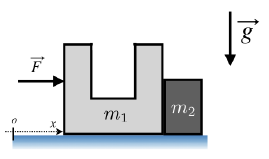
\includegraphics[width=0.7\textwidth]{classica-img/bloco1a.png} 
		\caption{Arranjo 1}
		\label{fig:bloco1apng}
	\end{minipage}\hfill
	\begin{minipage}{0.5\textwidth}
		\centering
		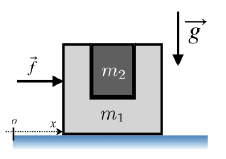
\includegraphics[width=0.7\textwidth]{classica-img/bloco2a.png}
		\caption{Arranjo 2}
		\label{fig:bloco2apng}
	\end{minipage}
\end{figure}

a) Indique esquematicamente todas as forças atuando em cada bloco da Figura 1.

\resposta

As figuras a baixo mostram as forças atuando em cada bloco.

\begin{figure}[H]
\centering
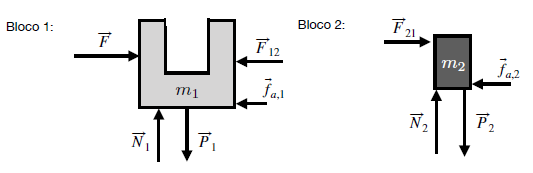
\includegraphics[scale=0.7]{classica-img/bloco1.png}
\end{figure}

As forças esquematizadas são as seguintes:

\begin{itemize}
\item[$\vec{F}_{ij}$]: Forças de contato entre os blocos (par de ação e reação: $\vec{F}_{ij}$ + $\vec{F}_{ji} = 0$).
\item[$\vec{f}_{a,i}$]: Força de atrito no $i$-ésimo bloco devido ao chão ($|\vec{f}_{a,i}| = \mu_{i} |\vec{N}_{i}|$).
\item[$\vec{N}_{i}$]: Força de reação normal no $i$-ésimo bloco devido ao chão.
\item[$\vec{P}_{i}$]: Força peso no $i$-ésimo bloco ($\vec{P}_{i} = m_{i}\vec{g}$).
\end{itemize}



b) Encontre a aceleração do bloco $m_{1}$ no caso da Figura \ref{bloco1png}. Dê sua resposta final em termos de $m_{1}$, $m_{2}$, $\mu_{1}$, $\mu_{2}$, $g$ e $F(x)$.

\resposta

Aplicando a segunda lei de Newton a cada um dos blocos e usando que os blocos movem-se com a mesma aceleração horizontal $a_{x}$

\begin{itemize}
\item na direção de x: $F(x) - F_{1,2} - f_{a,1} = m_{1}a_{x}$ \quad e \quad $F_{2,1} - f_{a,2} = m_{2}a_{x}$,

\item na direção y: $N_{1} = P_{1} \Rightarrow N_{1} = m_{1}g $ \quad e \quad $N_{2} = P_{2} \Rightarrow N_{2} = m_{2}g $.

$$
\left\{
\begin{array}{ccc}
	F(x) - F_{1,2} - f_{a,1} & = & m_{1} a_{x} \\
	       F_{2,1} - f_{a,2} & = & m_{2} a_{x}
\end{array}
\right.
$$

Do sistema acima as forças de contato se anulam. Isolando $a_{x}$

$$
\Rightarrow a_{x}  = \frac{F(x) - g(\mu_{1}m_{1} + \mu_{2} m_{2})}{m_{1} + m_{2}}
$$
\end{itemize}

c) Encontre a variação da energia cinética do arranjo da Figura 1 se a posição do bloco de massa $m_{1}$ variar de $x_{1}$ até $x_{2}$ ($x_{2} > x_{1}$) e se $F(x) = \alpha x$, onde $\alpha$ é uma constante positiva.

\resposta

Do teorema trabalho-energia cinética, sabe-se que a variação total da energia cinética é igual ao trabalho da força resultante $\vec{F}_{R}$ sobre o sistema. Esta é dada por

$$
\vec{F}_{R} = [F(x) - g(\mu_{1}m_{1} + \mu_{2}m_{2})] \hat{x}
$$

$$
\vec{F}_{R} = [\alpha x - g(\mu_{1}m_{1} + \mu_{2}m_{2})] \hat{x}.
$$

Segue que a variação da energia cinética $\Delta K$ entre as posições $x_{1}$ e $x_{2}$ é

$$
\Delta K = \int_{x_{2}}^{x_{1}} \vec{F}_{R} \cdot d\vec{l} = \frac{\alpha}{2} (x_{2}^{2} - x_{1}^{2}) - g(\mu_{1}m_{1} + \mu_{2}m_{2})(x_{2} - x_{1})
$$

d) Considere agora que ambos os conjuntos das Figuras 1 e 2 se movam instantaneamente com a mesma velocidade $v$ e que a potência dissipada por atrito no arranjo da Figura 2 seja o dobro da do arranjo da Figura 1. Encontre a razão $\mu_{2}/\mu_{1}$.

\resposta

A potência total instantânea dissipada pelo atrito é $P = \vec{f}_{a,tot} \cdot \vec{v} = - f_{a,tot} v$, onde $\vec{f}_{a,tot}$ é a força de atrito total atuando no sistema. Impondo-se a condição do enunciado $P_{fig,2} = 2P_{fig,1}$ e usando

$$
 \vec{f}_{a,tot,fig,1} = \vec{f}_{a,1} + \vec{f}_{a,2} = g(\mu_{1}m_{1} + \mu_{2}m_{2})\hat{x} \Rightarrow \mbox{Arranjo da Fig 1}
$$

$$
 \vec{f}_{a,tot,fig,2} = g\mu_{1}(m_{1} + m_{2}) \hat{x} \Rightarrow \mbox{Arranjo da Fig 2}
$$

Como $P_{fig,2} = 2P_{fig,1}$ obtém-se

$$
\mu_{1}(m_{1} + m_{2}) = 2(\mu_{1}m_{1} + \mu_{2}m_{2}) \Rightarrow \frac{\mu_{2}}{\mu_{1}} = \frac{m_{2} - m_{1}}{2m_{2}}
$$



\item Um pêndulo de comprimento l e massa $m$ está preso a um bloco de massa $M$. O bloco é livre para se mover sem atrito ao longo de um trilho horizontal, conforme indicado na figura. Considere a posição $y = 0$ ($\theta = \pi/2$) como o zero de energia potencial gravitacional. A aceleração da gravidade é $g$.

\begin{figure}[H]
\centering
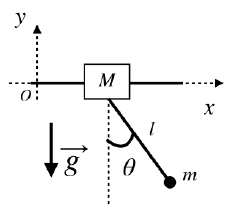
\includegraphics[scale=0.5]{classica-img/pendulo.png}
\end{figure}


a) Escreva a lagrangiana do sistema em termos das coordenadas generalizadas $x$ (posição do bloco) e $\theta$ (ângulo que o pêndulo faz com a vertical) mostradas na figura. Encontre as equações de movimento.

\resposta

No sistema de referência do enunciado, as posições do bloco de massa $M$ e da massa do pêndulo $m$ são dadas, respectivamente, por $\vec{r}_{M} = x(t)\hat{i}$ e $\vec{r}_{m} = [x(t) + l sen\theta(t)]\hat{i} - l cos\theta(t)\hat{j}$. Deste modo,

$$
v_{m}^{2} = \left| \frac{d\vec{r}_{m}}{dt} \right|^{2} = \left( \dot{x} + l\dot{\theta} cos \theta  \right)^{2} + \left( l\dot{\theta} sen \theta \right)^{2} = \dot{x}^{2} + l^{2} \dot{\theta}^{2} + 2 l\dot{\theta}\dot{x}cos \theta
$$

Portanto, adotando a posição $y = 0$ ($\theta = \pi/2$) como o zero de energia potencial gravitacional, a lagrangiana do sistema é dada por

$$
L = \frac{1}{2} M \dot{x}^{2} + \frac{1}{2} m \left( \dot{x}^{2} + l^{2} \dot{\theta}^{2} 2 l\dot{\theta}\dot{x}cos \theta   \right) + mlg \ cos \theta.
$$

Das equações de Euler-Lagrange, as equações de movimento são

\begin{eqnarray}
(m + M) \ddot{x} + (ml \cos \theta) \ddot{\theta} - (ml \ sen \theta) \dot{\theta}^{2} &=& 0 \\
l \ddot{\theta} + cos \theta \ddot{x} + g sen \theta &=& 0
\end{eqnarray}


b) Além da energia mecânica total, existe alguma outra constante de movimento na dinâmica do sistema?          Qual? Justifique.

\resposta

Sim, a componente $x$ do momentum linear total do sistema $P_{x}$ se conserva. Isto decorre do fato de que a força total no sistema só tem componente na direção $y$. De fato,

\begin{eqnarray*}
P_{x} &=& (\vec{p}_{M} + \vec{p}_{m})\cdot \hat{i} = M\dot{x} + m (\dot{x} + l \dot{\theta} cos \theta) \\
\Rightarrow \frac{dP_{x}}{dt} &=& (m+M)\ddot{x} + (mlcos\theta)\ddot{\theta} - (mlsen\theta)\dot{\theta}^{2} = 0,
\end{eqnarray*}

onde usamos a Eq. (1) no último passo. Alternativamente, percebe-se que a coordenada $x$ é ignorável, ou seja, a lagrangiana não depende de $x$. Portanto, o momento canonicamente conjugado a $x$, que é o lado esquerdo da Eq. (1), é conservado.


c) Considerando o regime de pequenas oscilações ($\theta << 1$), encontre o modo normal de oscilação do sistema e a sua frequência.

\resposta

Com $\theta << 1$ ($sen \theta \approx \theta$ e $cos \theta \approx 1$), as equações de movimento podem ser linearizadas

\begin{eqnarray}
(m+M)\ddot{x} + ml\ddot{\theta} &\approx & 0, \\
\ddot{x} + l\ddot{\theta} + g \theta &=& 0.
\end{eqnarray}

Isolando a equação para $\theta$, obtém-se

$$
\ddot{\theta} + \left( \frac{m+M}{M}  \right) \frac{g}{l} \theta = 0,
$$


cuja solução geral é $\theta (t) = A cos (\omega t + \varphi)$, onde $\omega = \sqrt{\frac{m+M}{M} \frac{g}{l}}$ e $A$ e $\varphi$ são constantes determinadas pelas condições iniciais. Integrando duas vezes a Eq. (3) em relação ao tempo obtém-se

$$
x(t) = -\frac{ml}{m+M} \theta l + Bt + C,
$$

Nesse modo, o bloco $M$ e a massa $m$ oscilam com a mesma frequência $\omega$ mas em sentidos opostos (além de um movimento do centro de massa do sistema com velocidade constante na direção $x$).



d) Além do caso trivial no qual o sistema está parado ($\dot{x} = 0$, $\dot{\theta} = 0$), existe algum outro movimento possível em que o pêndulo não oscile? Qual? Justifique.

\resposta

Sim. Fazendo $A = 0$ na solução do item (c), obtém-se $\theta(t) = 0$ e $x(t) = Bt + C$, isto é, o sistema se move com um todo com velocidade constante $B$, com o pêndulo sempre na vertical $\theta = 0$. Este é o outro modo normal do problema, cuja frequência de oscilação é nula. Deve-se notar que essa é uma solução exata das Eqs. de movimento (1) e (2).






\item A figura abaixo mostra esquematicamente um sistema formado pelo bloco 1, de massa $m_{1} = 2m$, conectado a uma mola de constante elástica $k$ e massa desprezível, e pelo bloco 2, de massa $m_{2} = m$. No instante inicial o bloco 1 está em repouso, a mola encontra-se relaxada, e o bloco 2 movimenta-se em direção ao bloco 1 com velocidade $\vec{v}_{2,1} = - v_{0} \hat{x}$, sendo $v_{0} > 0$. Os dois blocos colidem elasticamente elasticamente e o bloco 1 passa a oscilar após a colisão. Há atrito entre os blocos e a superfície \textbf{apenas no trecho inclinado AB} e o módulo da aceleração da gravidade vale $g$.

\begin{figure}[H]
\centering
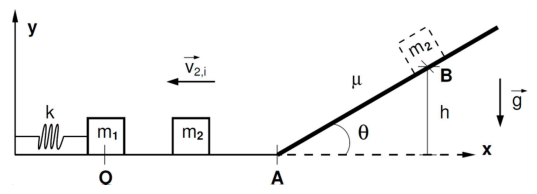
\includegraphics[scale=0.5]{classica-img/inclinado.png}
\end{figure}


a) Determine, em termos de $v_{0}$, os \textbf{vetores} velocidade dos blocos 1 e 2 imediatamente após a colisão ($\vec{v}_{1,f}$ e $\vec{v}_{2,f}$). Assuma que a mola não afeta o processo de colisão.

\resposta


b) Determine a amplitude $x_{m}$ do movimento oscilatório do bloco 1 após a colisão em termos de $m$, $k$ e $v_{0}$.

\resposta

c) Após a colisão, o bloco 2 movimenta-se em direção ao plano inclinado e atinge o repouso permanente no ponto B. Determine o coeficiente de atrito cinético $\mu$ entre o bloco 2 e o trecho inclinado AB em termos de $g$, $v_{0}$, da altura $h$ e do ângulo $\theta$

\resposta

d) Indique esquematicamente todas as forças que atuam no bloco 2 quando ele se encontra em repouso no ponto B.

\resposta



\item Uma barra longa e de massa desprezível movimenta-se no plano xy girando em torno do eixo z com velocidade angular constante $\omega$, como mostrado na figura abaixo. Uma partícula de massa $m$ pode deslizar sem atrito ao longo da barra, e sofre a ação de uma força externa $\vec{F} = m\gamma \hat{x}$, sendo $\gamma$ uma constante positiva.

\begin{figure}[H]
\centering
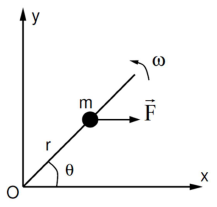
\includegraphics[scale=0.8]{classica-img/barra.png}
\end{figure}



a) Determine a energia potencial $V(\vec{r})$ associada à força $\vec{F}$. Considere a origem O como sendo o ponto de energia potencial nula.

\resposta

b) Determine a equação do vínculo em termos das coordenadas polares, $r$ e $\theta$, e do tempo $t$. Qual é a origem física da correspondente força de vínculo?

\resposta

c) Escreva a Lagrangiana da partícula em termo da coordenada $r$, da sua derivada temporal $\dot{r}$, e do tempo $t$. Em seguida, determine a correspondente equação de movimento.

\resposta

d) Considere o caso em que $\gamma = 0$ e determine a solução geral da equação de movimento calculada no item (c). Em seguida, determine a componente radial $r(t)$ da posição da partícula em funão do tempo. Incialmente, $r(t=0)=a$ e $\dot{r}(t=0)=0$.

\resposta




\item Um carro se move numa pista circular inclinada de um ângulo $\theta$ em relação à horizontal. A figura abaixo mostra o plano transversal ao movimento do carro. O módulo da aceleração da gravidade é $g$.
\begin{figure}[H]
\centering
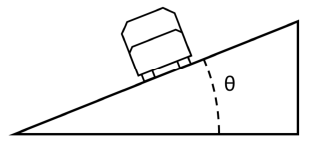
\includegraphics[scale=0.8]{classica-img/inclina}
\end{figure}



a) Indique esquematicamente todas as forças que atuam no carro, se o atrito for desprezível.

\resposta As forças que atuam no carro são a normal $\mathbb{N}$ e o peso $\mathbb{P}$, como mostrado na figura abaixo.
\begin{figure}[H]
\centering
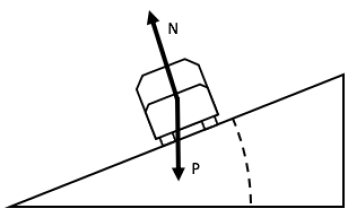
\includegraphics[scale=0.8]{classica-img/inclina1}
\end{figure}


b) Ainda desprezando o atrito, encontre o módulo da velocidade com a qual o carro se move, se ele descreve um círculo de raio $R$.

\resposta Tomando um sistema de referência fixo na pista e com origem na posição instantânea do carro com o eixo $z$ na direção vertical, teremos equilíbrio na direção $z$
$$
N \cos \theta = m g
$$
onde $m$ é a massa do carro. No plano $xy$ o carro realiza um movimento circular uniforme com velocidade $v$ cuja resultante centrípeta é
$$
N \sin \theta = \frac{mv^{2}}{R}.
$$
Eliminando $\mathbf{N}$ das Eqs. (1) e (2),
$$
v = \sqrt{gR\tan \theta}
$$

c) A partir deste item, considere que haja atrito entre os pneus do carro e a pista e que o coeficiente de atrito estático seja $\mu$. Se o carro se move com a velocidade máxima possível sem derrapar, indique esquematicamente todas as forças que atuam no carro.

\resposta Se $\mathbf{F}_{at}$ é a força de atrito, o diagrama de forças agora é
\begin{figure}[H]
\centering
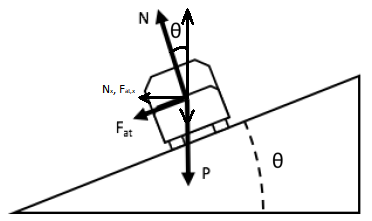
\includegraphics[scale=0.8]{classica-img/inclina2}
\end{figure}



d) Qual é o módulo da velocidade máxima com a qual o carro é capaz de fazer a curva de raio $R$ sem derrapar?

\resposta Usando o mesmo sistema de referência do item (b), ainda há equilíbrio na direção $z$
$$
N \cos \theta=m g+F_{a t} \sin \theta=m g+\mu N \sin \theta
$$
onde já usamos que, no limiar da derrapagem, a força de atrito estático $F_{at}$ atinge seu valor máximo, $\mu N$. A resultante centrípeta no plano $xy$ agora é
$$
N \sin \theta+F_{a t} \cos \theta=N \sin \theta+\mu N \cos \theta=\frac{m v_{\max }^{2}}{R}
$$
onde $v_{max}$ é a velocidade máxima sem derrapar. Eliminando novamente $N$ das Eqs. (3) e (4),
$$
v_{\max }=\sqrt{g R\left(\frac{\tan \theta+\mu}{1-\mu \tan \theta}\right)}.
$$

e) Suponha agora que $sin \ \theta > \mu cos \theta$ e que o carro se mova bem mais lentamente. Indique esquematicamente todas as forças que atuam no carro nesse caso. Determine a velocidade mínima com a qual o carro consegue descrever o círculo de raio $R$ sem derrapar.

\resposta Nesse caso, o sentido da força de atrito se inverte
\begin{figure}[H]
\centering
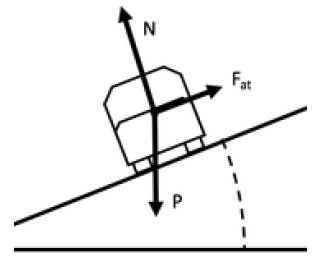
\includegraphics[scale=0.8]{classica-img/inclina3}
\end{figure}
O desenvolvimento do item (d) se repete bastando inverter o sinal de $\mu \rightarrow - \mu$ e a velocidade máxima sem derrapar $v_{min}$ é
$$
v_{\min }=\sqrt{g R\left(\frac{\tan \theta-\mu}{1+\mu \tan \theta}\right)}
$$
Note que o enunciado diz que $\tan \theta > \mu$, o que garante que o resultado obtido é um número real. Do contrário, o carro consegue ficar em repouso na pista, pois o ângulo é menor que o ângulo crítico $\theta_{c} = \arctan(\mu)$ e $v_{min} = 0$.







\item Considere um pêndulo constituído por um pequeno corpo de massa $m$ suspenso por uma mola de massa desprezível e constante elástica $k$. O comprimento de equilíbrio da mola (sem nenhuma massa pendurada) é $l$. Considere que o movimento do pêndulo esteja sempre contido num plano vertical fixo. Utilize coordenadas generalizadas tais que o comprimento da mola seja $l + r(t)$ e o ângulo desta com a vertical seja $\theta(t)$.


a) Escreva a energia cinética do sistema em termos de $r$, $\theta$ e suas derivadas temporais.

\resposta Suponha um sistema de referência tal que o plano $xy$ contenha o movimento do pêndulo, que sua origem esteja no ponto de sustentação do pêndulo e que o eixo $y$ seja vertical para cima. As relações entre as coordenadas cartesianas do corpo e $r$ e $\theta$ são
$$
x=(l+r) \sin \theta \ \ \ \mbox{e} \ \ \ y=-(l+r) \cos \theta
$$
A energia cinética assume a forma
$$
T=\frac{1}{2} m v^{2}=\frac{1}{2} m\left(\dot{x}^{2}+\dot{y}^{2}\right)=\frac{1}{2} m\left(\dot{r}^{2}+(r+l)^{2} \dot{\theta}^{2}\right)
$$

b) Escreva a energia potencial do sistema em termos de $r$, $\theta$ e suas derivadas temporais.

\resposta A energia potencial do sistema está associada à mola, $U_{mola}$, e ao campo gravitacional $g = - g \hat{y}$, $U_{g}$. Como o comprimento de equilíbrio da mola é igual a $l$
$$
U_{mola} = \frac{1}{2} kr^{2} \  \  \  \mbox{e} \  \  \ U_{g} = mgy = - mg(r+l)\cos \theta.
$$
Dessa forma,
$$
U = U_{mola} + U_{g} = \frac{1}{2} kr^{2} - mg(r+l)\cos \theta.
$$


c) Escreva a lagrangiana do sistema.

\resposta  Utilizando os resultados dos itens (a) e (b) a lagrangiana da partícula é dada por
$$
L = T - U = \frac{1}{2}m \left( \dot{r}^{2} + (r+l)^{2} \dot{\theta}^{2} \right) - \frac{1}{2} kr^{2} + mg(r+l)\cos \theta.
$$



d) Escreva as equações de Euler-Lagrange para $r$ e $\theta$.

\resposta Primeiramente,

$$
\begin{aligned}
\frac{\partial L}{\partial r} &=m(r+l) \dot{\theta}^{2}-k r+m g \cos \theta \\
\frac{\partial L}{\partial \dot{r}} &=m \dot{r} \\
\frac{\partial L}{\partial \theta} &=-m g(r+l) \sin \theta \\
\frac{\partial L}{\partial \dot{\theta}} &=m(r+l)^{2} \dot{\theta}
\end{aligned}
$$
As Eqs. de Euler-Lagrange são
$$
\begin{aligned}
&\frac{\partial L}{\partial r}-\frac{d}{d t}\left(\frac{\partial L}{\partial \dot{r}}\right)=0 \rightarrow \ddot{r}-(r+l) \dot{\theta}^{2}-g \cos \theta+\frac{k}{m} r=0\\
&\frac{\partial L}{\partial \theta}-\frac{d}{d t}\left(\frac{\partial L}{\partial \dot{\theta}}\right)=0 \quad \rightarrow \quad(r+l) \ddot{\theta}+2 \dot{r} \dot{\theta}+g \sin \theta=0
\end{aligned}
$$

e) Considere agora o movimento puramente vertical do pêndulo, ou seja, $\theta(t) = 0$ para todo $t$. Encontre a solução geral (em termos de duas constantes arbitrárias) da equação de Euler-Lagrange para $r$.

\resposta A equação de movimento (5) para $\theta = \dot{\theta} = 0$ assume a forma
$$
\ddot{r} + \frac{k}{m} r = g.
$$
A solução geral da Eq. (7) é dada por
$$
r(t) = r_{H}(t) + r_{P}(t)
$$
onde $r_{H}(t)$ é a solução geral da equação homogênea (ou seja, fazendo $g = 0$ na Eq. (7)) e $r_{P}(t)$ é uma solução particular qualquer da equação não homogênea. Como a equação homogênea é igual à equação de movimento do oscilador harmônico simples, temos que
$$
r_{H}(t) = A \cos \omega t + B \sin \omega t,
$$
onde $\omega = \sqrt{k/m}$ e $A$ e $B$ são constantes arbitrárias determinadas a partir das condições iniciais. Como o termo não homogêneo é constante, tentamos uma solução da forma
$$
r_{P}(t) = Ct^{2} + Dt + E.
$$
Substituindo na Eq. (7), verifica-se que as constantes $C = D = 0$ e $E = g/\omega^{2} = mg/k$. Assim,
$$
r_{P}(t) = \frac{g}{\omega^{2}} = \frac{mg}{k}.
$$
Por fim, a solução geral da Eq. (7) é dada por
$$
r(t) = A \cos \omega t + B \sin \omega t + \frac{mg}{k}.
$$








\item Uma partícula de massa $m$  movimenta-se num plano vertical (plano $xz$, sendo $x$ a direção horizontal e $z$ a direção vertical) sob a ação da força gravitacional $\mathbf{F}_{g} = m \mathbf{g} = - m g \hat{\mathbf{z}}$, onde $g$ é a aceleração da gravidade. No instante inicial $t=0$, a partícula está na origem e sua velocidade é $\mathbf{v}_{0} = (v_{0} cos \theta) \hat{\mathbf{x}} + (v_{0} sen \theta) \hat{\mathbf{z}}$, onde $v_{0} > 0$ e $0 < \theta < \pi/4$.



a) Escreva as equações de movimento para as componentes $x$ e $z$ da posição da partícula.

\resposta

b) Determine as componentes $v_{x}(t)$ e $v_{z}(t)$ da velocidade da partícula como funções do tempo.

\resposta

c) Determine as componentes $x(t)$ e $z(t)$ da posição da partícula como funções do tempo.

\resposta

d) Determine o \textbf{vetor} momento angular $\mathbf{L}(t)$ da partícula em relação à origem como função do tempo.

\resposta

e) Determine o \textbf{vetor} torque $\mathbf{N}(t)$ em relação à origem associado à força gravitacional $\mathbf{F}_{g}$ (como função do tempo) e encontre a relação entre $\mathbf{L}(t)$ e $\mathbf{N}(t)$.

\resposta




\item Uma partícula de massa $m$ movimenta-se em duas dimensões (plano $xy$) sob a ação de duas forças conservativas cujos potenciais são

$$
U_{1}(y) = \lambda y \quad  \mbox{ e } \quad U_{2}(r) = \frac{1}{2} kr^{2},
$$

onde $\lambda$ e $k$ são constantes positivas e $r = \sqrt{x^{2} + y^{2}}$ é a distância da partícula à origem do sistema de coordenadas.


a) Determine o \textbf{vetor} força $\mathbf{F}_{2}$ associada ao potencial $U_{2}(r)$.

\resposta

b) Escreva a lagrangiana da partícula utilizando coordenadas polares no plano $r$ e $\theta$ e determine as equações de movimento correspondentes.

\resposta

c) Encontre a hamiltoniana do sistema. Lembre-se de que a hamiltoniana deve ser escrita dem termos das coordenadas $r$ e $\theta$ e dos seus momentos canonicamente conjugados.

\resposta

d) Encontre o \textbf{vetor} momento angular $\mathbf{L}$ em termos das coordenadas polares $r$ e $\theta$. Determine sob qual condição o momento angular da partícula é conservado.

\resposta




\item Um disco fino homogêneo de raio $R$ e massa m move-se ao longo de uma superfície horizontal. O coeficiente de atrito cinético entre o disco e a superfície horizontal é $\mu$. No instante inicial (ver figura abaixo), a coordenada $x$ do centro do disco está em O, a velocidade do seu centro
$\mathbf{v}_{0} = v_{0}\hat{\mathbf{x}}$ e a velocidade angular de rotação (em torno do eixo que passa pelo centro de massa e é normal ao disco) é nula. \textbf{Apenas quando atinge o ponto A o disco passa a rolar sem deslizar}: enquanto a coordenada $x$ do seu centro percorre o trecho de O até A, a
força de atrito cinético age de forma a mudar tanto a velocidade do centro de massa quanto a velocidade angular de rotação. Considere que o plano do disco se mantém paralelo ao plano $xy$ e a aceleração da gravidade é $\mathbf{g} -g\hat{\mathbf{y}}$.

\begin{figure}
\centering
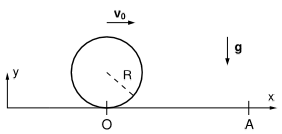
\includegraphics[scale=1]{classica-img/disco.png}
\end{figure}


a) Indique esquematicamente todas as forças que atuam sobre o disco no trecho OA.

\resposta

b) Determine os \textbf{módulos} das acelerações linear $a$ e angular $\alpha$ do disco em termos de $R$, $\mu$ e $g$ no trecho OA. O momento de inércia do disco em relação ao eixo que passa pelo seu centro e é normal ao plano do disco é $I = mR^{2}/2$.

\resposta

c) Determine os \textbf{módulos} das velocidades linear $v$ e angular $\omega$ do disco para o trecho OA como funções do tempo.

\resposta

d) Escreva a relação entre os \textbf{módulos} das velocidades linear $v$ e angular $\omega$ do disco quando ele passa a rolar sem deslizar (ponto A). Em seguida, determine o instante de tempo $t_{A}$ em que a coordenada $x$ do centro do disco atinge o ponto A. Expresse sua resposta em termos de $v_{0}$, $\mu$ e $g$.

\resposta







\item Considere uma partícula de massa $m$ que se movimenta na superfície interna de um cone cuja ponta é a origem do sistema de coordenadas e cujo eixo é o semi-eixo $z > 0$. A equação da superfície do cone em coordenadas cilíndricas ($\rho, \varphi e z$) é $z = \rho$. A partícula está sob a ação do campo gravitacional $\mathbf{g} = —g\hat{\mathbf{z}}$.


a) Escreva a lagrangiana da partícula em termos de $\rho, \varphi, \dot{\rho} e \dot{\rho}$

\resposta

b) Determine as equações de movimento da partícula.

\resposta

c) Calcule o $\mathbf{vetor}$ momento angular da partícula $\mathbf{L}$ em termos das coordenadas cilíndricas $\rho$, $\phi$ e $z$ e dos vetores unitários $\hat{\mathbf{\rho}}$, $\hat{\mathbf{\phi}}$ e $\hat{\mathbf{z}}$. Determine qual componente de $\mathbf{L}$ é conservada.

\resposta

d) A partir das equações de movimento derivadas no item (b), mostre que a partícula pode apresentar uma órbita circular de raio $\rho_{0}$. Determine a frequência angular dessa órbita em termos de $g$ e $\rho_{0}$ Determine a frequência angular dessa órbita em termos de $g$ e $\rho_{0}$.

\resposta





\item Um corpo de massa $m$ cai em linha reta a partir do repouso em um fluido. A aceleração da gravidade $\vec{g}$ pode considerada constante. O corpo é sujeito também a uma força de resistência proporcional à velocidade: $\vec{F}_{r} = -km\vec{v}$, onde $k$ é uma constante. A força de empuxo do fluido é desprezível.


a) Obtenha o módulo da velocidade do corpo como função do tempo.

\resposta Da componente da segunda lei de Newton na direção vertical (orientada para cima), a queda é descrita por
$$
F=m \frac{d v}{d t}=-m g-k m v \Rightarrow \frac{d v}{d t}=-(g+k v) \Rightarrow \int_{0}^{v} \frac{d v^{\prime}}{g+k v^{\prime}}=-\int_{0}^{t} d t^{\prime}
$$
onde usamos a condição inicial de que o corpo parte do repouso. Usando
$$
\int \frac{d x}{a x+b}=\frac{1}{a} \ln (a x+b)
$$
segue que
$$
\int_{0}^{v} \frac{d v^{\prime}}{g+k v^{\prime}}=-\int_{0}^{t} d t^{\prime} \Rightarrow \ln \left(\frac{g+k v}{g}\right)=-k t
$$
Invertendo a última relação
$$
v(t)=\frac{g}{k}\left(e^{-k t}-1\right)
$$
Como $v(t)<0$ (corpo em queda), o módulo da velocidade é
$$
|v(t)|=-\frac{g}{k}\left(e^{-k t}-1\right)=\frac{g}{k}\left(1-e^{-k t}\right)
$$

b) Qual é a velocidade terminal do corpo (módulo da velocidade no limite $t \rightarrow \infty$)?

\resposta A velocidade terminal $v_{\text {term}}$ é obtida tomando-se o limite $t \rightarrow \infty$ na Eq. (3)
$$
v_{\text {term}}=\lim _{t \rightarrow \infty} \frac{g}{k}\left(e^{-k t}-1\right)=-\frac{g}{k} \Rightarrow\left|v_{\text {term}}\right|=\frac{g}{k}
$$

c) Encontre $z(t)$, a posição do corpo como função do tempo (considere $z(0) = 0$).

\resposta A posição vertical do corpo é obtida integrando mais uma vez a Eq.
$$
v=\frac{d z}{d t}=\frac{g}{k}\left(e^{-k t}-1\right) \Rightarrow \frac{k}{g} \int_{0}^{z} d z^{\prime}=\int_{0}^{t}\left(e^{-k t^{\prime}}-1\right) d t^{\prime} \Rightarrow \frac{k z}{g}=-\frac{e^{-k t}}{k}+\frac{1}{k}-t
$$
donde
$$
z(t)=\frac{g}{k^{2}}\left(1-e^{-k t}\right)-\frac{g t}{k}
$$

d) Encontre $z(v)$, a posição do corpo como função do módulo da velocidade.

\resposta Das Eqs. (3) e (4)
$$
z=-\frac{v}{k}-\frac{g}{k} t
$$
Eliminando $t$ usando a Eq. $(2),$ encontramos a expressão procurada
$$
z(v)=\frac{g}{k^{2}} \ln \left(1+\frac{k v}{g}\right)-\frac{v}{k}
$$
Alternativamente, da Eq. ( 1 )
$$
a=\frac{d v}{d t}=-(g+k v)
$$
Mas
$$
\frac{d v}{d z}=\frac{d v}{d t} \frac{d t}{d z}=\frac{a}{v} \Rightarrow v d v=a d z=-(g+k v) d z
$$
Logo
$$
-\int_{0}^{v} \frac{v^{\prime}}{g+k v^{\prime}} d v^{\prime}=\left.\int_{0}^{z} d z^{\prime} \Rightarrow \frac{g \ln (g+k v)-k v}{k^{2}}\right|_{0} ^{v}=\left.z\right|_{0} ^{z}
$$
onde usamos o resultado $\int \frac{x}{a+b x} d x=\frac{b x-a \ln (a+b x)}{b^{2}} .$ Segue que
$$
z(v)=\frac{g}{k^{2}} \ln \left(1+\frac{k v}{g}\right)-\frac{v}{k}
$$




\item O pêndulo duplo plano consiste de duas partículas de massas $m_{1}$ e $m_{2}$ e duas hastes rígidas de massas desprezíveis e comprimentos $l_{1}$ e $l_{2}$, que oscilam, sob a ação da gravidade $\vec{g}$, em um mesmo plano vertical fixo, como representado na figura abaixo. Considerando $\vec{g}$ constante e adotando como coordenadas generalizadas os ângulos $\theta_{1}$ e $\theta_{2}$ da figura, obtenha:

\begin{figure}[H]
\centering
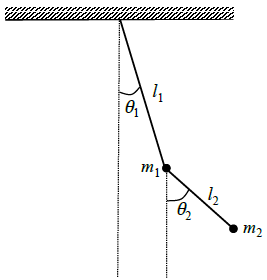
\includegraphics[scale=1]{classica-img/pendulo2.png}
\end{figure}


a) A energia cinética do sistema.

\resposta Seja um sistema cartesiano de coordenadas com $x$ na horizontal orientada para a direita e $y$ na vertical orientada para baixo e com a origem no ponto de sustentação do pêndulo superior. Sejam $\left(x_{1}, y_{1}\right) \mathrm{e}\left(x_{2}, y_{2}\right)$ as coordenadas cartesianas das partículas de massas $m_{1} \mathrm{e} m_{2}$ respectivamente. Então,
$$
x_{1}=l_{1} \sin \theta_{1}, \quad y_{1}=l_{1} \cos \theta_{1}, \quad x_{2}=l_{1} \sin \theta_{1}+l_{2} \sin \theta_{2}, \quad y_{2}=l_{1} \cos \theta_{1}+l_{2} \cos \theta_{2}
$$
donde
$$
\begin{aligned}
\dot{x}_{1} &=l_{1} \dot{\theta}_{1} \cos \theta_{1}, \quad \dot{x}_{2}=l_{1} \dot{\theta}_{1} \cos \theta_{1}+l_{2} \dot{\theta}_{2} \cos \theta_{2} \\
\dot{y}_{1} &=-l_{1} \dot{\theta}_{1} \sin \theta_{1}, \quad \dot{y}_{2}=-l_{1} \dot{\theta}_{1} \sin \theta_{1}-l_{2} \dot{\theta}_{2} \sin \theta_{2}
\end{aligned}
$$
A energia cinética da partícula $1 é$
$$
T_{1}=\frac{m_{1}}{2}\left(\dot{x}_{1}^{2}+\dot{y}_{1}^{2}\right)=\frac{m_{1}}{2}\left(l_{1}^{2} \dot{\theta}_{1}^{2} \cos ^{2} \theta_{1}+l_{1}^{2} \dot{\theta}_{1}^{2} \sin ^{2} \theta_{1}\right)=\frac{m_{1}}{2} l_{1}^{2} \dot{\theta}_{1}^{2}
$$
Para a partícula 2
$$
\begin{array}{l}
\dot{x}_{2}^{2}=l_{1}^{2} \dot{\theta}_{1}^{2} \cos ^{2} \theta_{1}+l_{2}^{2} \dot{\theta}_{2}^{2} \cos ^{2} \theta_{2}+2 l_{1} l_{2} \dot{\theta}_{1} \dot{\theta}_{2} \cos \theta_{1} \cos \theta_{2} \\
\dot{y}_{2}^{2}=l_{1}^{2} \dot{\theta}_{1}^{2} \sin ^{2} \theta_{1}+l_{2}^{2} \dot{\theta}_{2}^{2} \sin ^{2} \theta_{2}+2 l_{1} l_{2} \dot{\theta}_{1} \dot{\theta}_{2} \sin \theta_{1} \sin \theta_{2}
\end{array}
$$
donde
$$
T_{2}=\frac{m_{2}}{2}\left(\dot{x}_{2}^{2}+\dot{y}_{2}^{2}\right)=\frac{m_{2}}{2}\left[l_{1}^{2} \dot{\theta}_{1}^{2}+l_{2}^{2} \hat{\theta}_{2}^{2}+2 l_{1} l_{2} \dot{\theta}_{1} \dot{\theta}_{2} \cos \left(\theta_{1}-\theta_{2}\right)\right]
$$
A energia cinética total é
$$
T=T_{1}+T_{2}=\frac{m_{1}}{2} l_{1}^{2} \dot{\theta}_{1}^{2}+\frac{m_{2}}{2}\left[l_{1}^{2} \dot{\theta}_{1}^{2}+l_{2}^{2} \dot{\theta}_{2}^{2}+2 l_{1} l_{2} \dot{\theta}_{1} \dot{\theta}_{2} \cos \left(\theta_{1}-\theta_{2}\right)\right]
$$

b) A energia potencial do sistema.

\resposta A energia potencial é
$$
V=-m_{1} g y_{1}-m_{2} g y_{2}=-m_{1} g l_{1} \cos \theta_{1}-m_{2} g\left(l_{1} \cos \theta_{1}+l_{2} \cos \theta_{2}\right)
$$


c) A Lagrangiana do sistema.

\resposta A Lagrangiana é $L=T-V$
$$
\begin{aligned}
L &=\frac{m_{1}}{2}\left(l_{1}^{2} \dot{\theta}_{1}^{2}+2 g l_{1} \cos \theta_{1}\right) \\
&+\frac{m_{2}}{2}\left[l_{1}^{2} \dot{\theta}_{1}^{2}+l_{2}^{2} \dot{\theta}_{2}^{2}+2 l_{1} l_{2} \dot{\theta}_{1} \dot{\theta}_{2} \cos \left(\theta_{1}-\theta_{2}\right)+2 g\left(l_{1} \cos \theta_{1}+l_{2} \cos \theta_{2}\right)\right]
\end{aligned}
$$


d) As equações de movimento relativas a $\theta_{1}$ e $\theta_{2}$.

\resposta As equações de movimento são as equações de Euler-Lagrange
$$
\frac{d}{d t}\left(\frac{\partial L}{\partial \dot{\theta}_{i}}\right)-\frac{\partial L}{\partial \theta_{i}}=0 \quad(i=1,2)
$$
Temos para $i=1$
$$
\begin{aligned}
\frac{\partial L}{\partial \theta_{1}} &=-\left(m_{1}+m_{2}\right) g l_{1} \sin \theta_{1}-m_{2} l_{1} l_{2} \dot{\theta}_{1} \dot{\theta}_{2} \sin \left(\theta_{1}-\theta_{2}\right) \\
\frac{\partial L}{\partial \dot{\theta}_{1}} &=\left(m_{1}+m_{2}\right) l_{1}^{2} \dot{\theta}_{1}+m_{2} l_{1} l_{2} \dot{\theta}_{2} \cos \left(\theta_{1}-\theta_{2}\right)
\end{aligned}
$$
%
$$
\frac{d}{d t}\left(\frac{\partial L}{\partial \dot{\theta}_{1}}\right)=\left(m_{1}+m_{2}\right) l_{1}^{2} \ddot{\theta}_{1}+m_{2} l_{1} l_{2} \ddot{\theta}_{2} \cos \left(\theta_{1}-\theta_{2}\right)-m_{2} l_{1} l_{2} \dot{\theta}_{2} \sin \left(\theta_{1}-\theta_{2}\right)\left(\dot{\theta}_{1}-\dot{\theta}_{2}\right)
$$
e para $i=2$
$$
\begin{aligned}
\frac{\partial L}{\partial \theta_{2}} &=-m_{2} g l_{2} \sin \theta_{2}+m_{2} l_{1} l_{2} \dot{\theta}_{1} \dot{\theta}_{2} \sin \left(\theta_{1}-\theta_{2}\right) \\
\frac{\partial L}{\partial \dot{\theta}_{2}} &=m_{2} l_{2}^{2} \dot{\theta}_{2}+m_{2} l_{1} l_{2} \dot{\theta}_{1} \cos \left(\theta_{1}-\theta_{2}\right) \\
\frac{d}{d t}\left(\frac{\partial L}{\partial \dot{\theta}_{2}}\right)=& m_{2} l_{2}^{2} \ddot{\theta}_{2}-m_{2} l_{1} l_{2} \dot{\theta}_{1} \sin \left(\theta_{1}-\theta_{2}\right)\left(\dot{\theta}_{1}-\dot{\theta}_{2}\right)+m_{2} l_{1} l_{2} \ddot{\theta}_{1} \cos \left(\theta_{1}-\theta_{2}\right)
\end{aligned}
$$
As equações procuradas são, portanto,
$$
\begin{aligned}
\left(m_{1}+m_{2}\right)\left(l_{1}^{2} \ddot{\theta}_{1}+g l_{1} \sin \theta_{1}\right)+m_{2} l_{1} l_{2}\left[\ddot{\theta}_{2} \cos \left(\theta_{1}-\theta_{2}\right)+\dot{\theta}_{2}^{2} \sin \left(\theta_{1}-\theta_{2}\right)\right] &=0 \\
m_{2}\left[l_{2}^{2} \tilde{\theta}_{2}+g l_{2} \sin \theta_{2}\right]+m_{2} l_{1} l_{2}\left[\ddot{\theta}_{1} \cos \left(\theta_{1}-\theta_{2}\right)-\dot{\theta}_{1}^{2} \sin \left(\theta_{1}-\theta_{2}\right)\right] &=0
\end{aligned}
$$





\item A aceleração da gravidade $g$ pode ser medida com razoável precisão usando-se um pêndulo simples que consiste de um corpo de massa $m$ preso a um fio de massa desprezível e comprimento $l$.


a) Encontre a expressão do período do pêndulo em função dos seus parâmetros.

\resposta

b) Um grupo de estudantes foi ao laboratório para obter uma medida precisa da aceleração da gravidade no local. Para isso construiu um pêndulo simples com uma massa metálica presa ao teto do laboratório por um fio fino. A massa metálica tem a forma de uma esfera de raio $r = 8,00 \pm 0,05 \ cm$ e massa $m = 10,0 \pm 0,1 \ kg$ presa ao fio de forma que em repouso o centro de massa da esfera fica a $4,00 \pm 0,02 \ m$ do teto. A massa do fio é $7,4 \pm 0,2 \ g$. O período de oscilação foi medido para diferentes deslocamentos iniciais laterais entre $5,0 \pm 0,1$ e $10,0 \pm 0,1 \ cm$. Os estudantes determinaram que nesse intervalo de deslocamentos laterais o período n˜ao depende da posição inicial, dentro da incerteza experimental e que o pêndulo realizou 10 oscilações completas em $40,0 \pm 0,5 \ s$. Determine o valor de $g$ encontrado, com a incerteza experimental. Considere, se necessário, $\pi^{2} = 9,86960$.

\resposta




\item Dois corpos, cada um de massa $M$, est˜ao ligados por uma corda uniforme inextensível de comprimento l. O corpo $A$ está sobre uma mesa uniforme e o corpo $B$ está pendurado na lateral, a corda passando por uma polia de raio desprezível sem atrito, como mostrado na figura. Despreze o atrito entre $A$ e a mesa.

\begin{figure}[H]
\centering
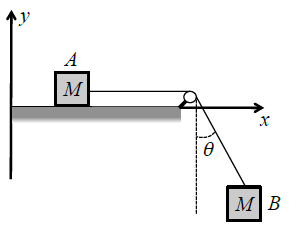
\includegraphics[scale=1]{classica-img/pendulo3.png}
\end{figure}


a) Encontre a aceleração comum dos corpos, se o ângulo $\theta$ é mantido constante e igual a zero e a massa da corda é desprezível.

\resposta

b) Considere agora o movimento mais geral em que o ângulo $\theta$ também pode variar. Suponha que $\theta$ é sempre menor que $\pi/2$ e que o corpo $B$ nunca toca na mesa. Escreva a Lagrangiana do sistema e as equações de movimento (não tente resolver as equações). Mostre que recuperamos o resultado do item (a) se fizermos $\theta = 0$.

\resposta

c) Suponha agora que $\theta$ é novamente mantido constante e igual a zero, mas a corda tem massa não desprezível $m$. Escreva a Lagrangiana do sistema e as equações de movimento. Não é necessário resolver as equações.

\resposta



\item Um disco de raio $R$ é composto por duas metades cada uma com densidades superficiais de massa respectivas de $1\rho$ e de $2\rho$.

\begin{figure}[H]
\centering
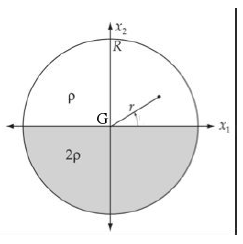
\includegraphics[scale=1]{classica-img/discoraio.png}
\end{figure}


a) Qual é o momento de inércia em relação ao eixo (perpendicular ao plano do disco) que passa pelo seu centro geométrico $G$?

\resposta

b) Encontre as coordenadas $x_{1}$ e $x_{2}$ do centro de massa do disco.

\resposta

c) Qual é o momento de inércia em relação ao eixo (perpendicular ao plano do disco) que passa pelo seu centro de massa?

\resposta

d) Considere o movimento em linha reta do disco sobre um plano horizontal perpendicular ao plano do disco, sem deslizar. Encontre $\lambda(\theta)$, implicitamente definido por
$$
v(t) = \lambda(\theta) R \frac{d\theta}{dt},
$$
onde $\theta$ é o ângulo entre o eixo vertical e a reta que passa pelo centro geométrico e o centro de massa (veja a figura), $v(t)$ é o módulo da velocidade do centro de massa, e $d\theta/dt$ é o módulo da velocidade de rotação do disco.
\begin{figure}[H]
\centering
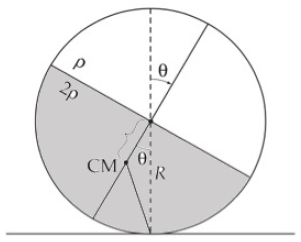
\includegraphics[scale=1]{classica-img/discoraio2.png}
\end{figure}

\resposta


\item Considere um objeto de massa $M$ que se desloca sob ação de uma força central do tipo coulombiana modificada por uma força proporcional ao inverso de $r^{3}$,
$$
F(r) = - \frac{k}{r^{2}} - \frac{q}{r^{3}},
$$
onde $r$ é a coordenada radial, e $k$ e $q$ são constantes positivas. Considere que a energia total do sistema é descrita por
$$
E = \frac{M}{2} \dot{r}^{2} + \frac{M}{2} r^{2} \dot{\theta}^{2} - \frac{k}{r} - \frac{q}{2r^{2}},
$$
e que o momento angular, do sistema é dado por $L = M r^{2} \dot{\theta}$.

a) Para o caso em que o objeto descreva uma órbita circular (de equilíbrio) encontre o raio da órbita em função dos parâmetros $k$, $q$, $M$ e $L$, do sistema.

\resposta

b) Para as mesmas condições do item (a), encontre a energia total, $E$, em função dos parâmetros
k, q, M e L, do sistema.

\resposta

c) Ao identificar o potencial efetivo para o movimento radial como
$$
V_{ef}(r) = \frac{L^{2}}{2mr^{2}} - \frac{k}{r} - \frac{q}{2r^{2}},
$$
verifique sob quais condições sobre as constantes $q$, $L$ e $M$, a coordenada radial da órbita circular obedece uma configuração de equilíbrio estável.

\resposta

d) No caso da coordenada radial da partícula se deslocar da condição de equilíbrio (estável) e passar a oscilar de forma aproximadamente harmônica (em torno do raio da órbita circular), encontre a relação entre o período de oscilação radial e o período de revolução (movimento angular) em função das constantes $q$, $M$ e $L$.

\resposta


\item Uma esfera de bronze sólida de massa $m$ e raio $r$ rola sem deslizar ao longo de um plano inclinado após ser solta do repouso de uma altura $h$. O momento de inércia da esfera em relação a um eixo que passa pelo seu centro é $I = 2mr^{2}/5$ e a aceleração da gravidade é $g$. O plano inclinado forma um ângulo $\theta$ com a horizontal, como mostra a figura.

\begin{figure}[H]
\centering
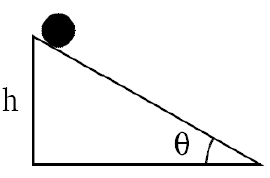
\includegraphics[scale=1]{classica-img/inclinado2.png}
\end{figure}


a) Há atrito entre a esfera e o plano inclinado? Como você chegou a essa conclusão?

\resposta Sim, pois a única força capaz de gerar o torque para que a esfera role sem deslizar é o atrito.

b) Há conservação de energia mecânica? Justifique sua resposta levando em consideração o respondido no item (a).

\resposta Sim, pois o atrito é estático e não realiza trabalho, uma vez que a velocidade do ponto de contato entre a esfera e o plano inclinado é nula (rolamento sem deslizamento).

c) Utilizando considerações de energia, determine a velocidade com que a esfera atinge a base do plano inclinado.

\resposta Tomando a base do plano como o zero de energia potencial gravitacional, a energia mecânica inicial é apenas potencial gravitacional, dada por $E_{i} = mgh$. Na base do plano inclinado, a energia mecânica é puramente cinética, dada pela energia cinética de translação do centro de massa (CM) mais a energia de rotação em torno do CM, ou seja, $E_{f} = mv^{2}/2 + I \omega^{2}/2$, onde $v$ e $\omega$ são, respectivamente, as velocidades de translação do CM e angular na base do plano. Por conservação de energia mecânica,
%
\begin{equation}
  mgh = \frac{1}{2} m v^{2} + \frac{1}{2} I \omega^{2} .
\end{equation}
%
Como há rolamento sem deslizamento, a velocidade de translação do CM e a velocidade de rotação satisfazem $v = \omega r$. Substituindo na Eq. (1) e usando a expressão para o momento de inércia dada no enunciado obtemos
%
\begin{equation}
  v = \sqrt{\frac{10}{7} gh }  .
\end{equation}
%


d) Obtenha a velocidade na base do plano inclinado já calculada no item (c) utilizando agora considerações de dinâmica (ou seja, aplicando a segunda lei de Newton).

\resposta Definimos um sistema de coordenadas com um eixo $x$ paralelo ao plano inclinado e apontando para a base do plano e um eixo $y$ perpendicular ao plano e apontando para cima do plano. A força resultante no eixo $y$ é nula. No eixo $x$, usando a segunda lei de Newton,
%
\begin{equation}\label{eq2}
  mg \sin \theta - f_{at} = ma ,
\end{equation}
%
onde $f_{at}$ é a força de atrito e $a$ a aceleração do CM. Para o movimento de rotação
%
\begin{equation}\label{eq3}
  \tau  = f_{at} r = I \alpha ,
\end{equation}
%
onde $\tau$ é o torque em relação a um eixo que passa pelo CM da esfera e $\alpha$ é sua aceleração angular. Derivando em relação ao tempo a expressão do item anterior, $v = \omega r$, obtemos $a = \alpha r$. Levando esta última relação e a Eq. (\ref{eq2}) na Eq. (\ref{eq3}) obtemos
\begin{equation}
  (mg \sin \theta - ma) r = \frac{2}{5} m r^{2} \frac{a}{r} ,
\end{equation}
%
donde
%
\begin{equation}\label{eq4}
  a = \frac{5}{7} g \sin \theta .
\end{equation}
%
Dado que $a$ é constante, podemos usar a seguinte relação, válida para um movimento uniformemente acelerado,
%
\begin{equation}\label{eq5}
\begin{array}{ccc}
  v^{2} & = & v_{o}^{2} 2 a \Delta x \\
        & = & 2ah / \sin \theta ,
\end{array}
\end{equation}
%
onde $v_{o} = 0$ é a velocidade no instante inicial e $\Delta x = h/\sin \theta$ o deslocamento no eixo $x$. Levando a Eq. (\ref{eq4}) na Eq. (\ref{eq5})
%
\begin{equation}
  v = \sqrt{\frac{10}{7} gh } ,
\end{equation}
%
que coincide com o resultado já encontrado no item (c).




\item Considere uma massa $m$ presa à extremidade de uma haste inextensível de massa desprezível e comprimento $l$. A outra extremidade da haste está presa a um ponto fixo e o sistema haste-massa move-se em um plano vertical num local onde a aceleração da gravidade é $g$.


a) Escreva a Lagrangiana do sistema.

\resposta Utilizaremos como coordenada generalizada o ângulo $\theta$ que a haste faz com a vertical. O módulo da velocidade da partícula é dado por $v = l \dot{\theta}$, de modo que sua energia cinética é
%
\begin{equation}
  T = \frac{m(l \dot{\theta})^{2}}{2} .
\end{equation}
%
A altura na vertical, em relação à posição em que $\theta = 0$, é dada por $h = l - l \cos \theta$. Segue que a energia potencial gravitacional é
%
\begin{equation}
  V = mgl(1 - \cos \theta)
\end{equation}
%
Finalmente, a Lagrangiana do sistema é
%
\begin{equation}\label{eq6}
  L = T - V = \frac{ml^{2} \dot{\theta}^{2}}{2} - mgl(1 - \cos \theta)
\end{equation}
%


b) Obtenha a equação de movimento que descreve o sistema.

\resposta A equação de movimento é obtida a partir da equação de Euler-Lagrange
%
\begin{equation}
  \frac{d}{dt} \left( \frac{\partial L}{\partial \dot{\theta}}  \right) - \frac{\partial L}{\partial \theta} = 0 .
\end{equation}
%
Utilizando a Eq. (\ref{eq6}) na equação acima, temos
\begin{equation}
  \ddot{\theta} = - \frac{g}{l} \sin \theta .
\end{equation}

c) Determine os pontos de equilíbrio do sistema e classifique-os quanto à estabilidade, justificando suas respostas.

\resposta Nos pontos de equilíbrio, $dV / d\theta = 0$, o que nos dá $\sin \theta = 0$, ou seja, os pontos procurados são
$$
\theta = 0 \ \ \ \mbox{e} \ \ \ \theta = \pi .
$$
Para avaliar a estabilidade dos pontos de equilíbrio, analisamos o sinal de
\begin{equation}
  \frac{d^{2}V}{d\theta^{2}} = mgl \cos \theta .
\end{equation}
%
Para $\theta = 0$, a expressão acima tem valor positivo (mínimo de $V$ ), caracterizando um equilíbrio estável, enquanto que para $\theta = \pi$, o sinal é negativo (máximo de $V$ ), correspondendo a um ponto de equilíbrio instável.

d) Encontre a frequência de pequenas oscilações em torno do ponto de equilíbrio estável

\resposta Para pequenas oscilações em torno de $\theta = 0$, podemos aproximar $\sin \theta \approx \theta$. A equação de movimento fica
%
\begin{equation}
  \ddot{\theta} = - \frac{g}{l} \theta ,
\end{equation}
%
cuja solução geral é, por inspeção,
\begin{equation}
  \theta (t) = A \sin (\omega t + \delta) ,
\end{equation}
%
onde $A$ e $\delta$ são constantes arbitrárias determinadas pelas condições iniciais e
%
\begin{equation}
  \omega = \sqrt{g/l} , 
\end{equation}
%
que é a frequência (angular) procurada. Alternativamente, pode-se comparar a Eq. (\ref{eq2}) com a equação de movimento de um oscilador harmônico simples uni-dimensional de frequência (angular) $\omega$,
%
\begin{equation}
  \ddot{x} + \omega^{2} x = 0
\end{equation}
%
e inferir que no caso em questão teremos $\omega = \sqrt{g/l}$




\item É possível construir armadilhas capazes de confinar íons de massa $m$ e carga $q$. Em particular, a armadilha pode restringir o movimento dos íons a apenas uma dada direção espacial, $x$. Assim, considere dois íons de cálcio uma vez ionizado ($Ca^{+}$), submetidos a um potencial confinante externo harmônico $U(x) = m\omega^{2}x^{2}/2$. Esses íons interagem adicionalmente através da repulsão coulombiana,
$$
F_{C} = \frac{e^{2}}{ \left( x^{1} - x^{2} \right)^{2} }
$$
onde $x_{1}$ e $x_{2}$ são as posições dos íons de cálcio e, por simplicidade, foi definido: $e^{2} = q^{2} / (4\pi \epsilon_{0})$.
\begin{figure}[H]
\centering
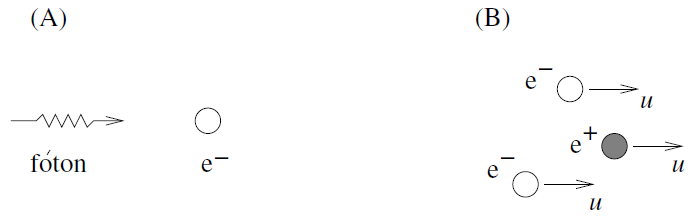
\includegraphics[scale=1]{classica-img/particula.png}
\end{figure}
A figura acima define um sistema de coordenadas conveniente e representa os íons na posição de equilíbrio em que $-x_{1} = x_{2} = x_{0}$. O objetivo deste problema é estudar os modos normais dessa cadeia unidimensional constituida pelos dois íons de cálcio.


a) Obtenha a posição de equilibrio $x_{0}$ em termos de $e$, $m$ e $\omega$.

\resposta


b) Escreva as equações de Newton para o movimento de cada íon e obtenha a frequência de oscilação do sistema quando a separação entre os íons for constante. Este é o primeiro modo normal de oscilação dessa cadeia.

\resposta

c) O segundo modo normal corresponde a um movimento antissimétrico dos íons, em cujo caso o centro de massa está parado em $x = 0$. Obtenha esse segundo modo normal no limite de pequenas oscilações. Obtenha a razão entre as frequências dos dois modos normais de oscilação do sistema.

\resposta

d) As figuras a) e b) abaixo representam os modos normais de oscilação desse sistema de dois íons. Identifique o primeiro e o segundo modo normal obtidos, respectivamente, nos itens (b) e (c) acima. Qual deles tem menor energia?

\begin{figure}[H]
\centering
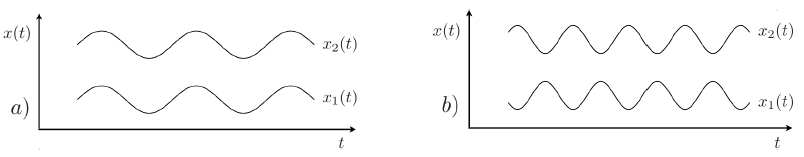
\includegraphics[scale=0.7]{classica-img/ondas.png}
\end{figure}

\resposta

\item Um satélite artificial de massa $m$ está em órbita elíptica em torno da Terra. Admita que a Terra seja uma esfera de densidade uniforme com raio $R$ e massa $M$, e denote por $G$ a constante de gravitação universal. Considere conhecidos $d$ e $D$, as distâncias entre o centro da Terra e o satélite nos pontos de menor e maior afastamento, respectivamente. Uma partícula de massa $m_{0}$ menor do que $m$, choca-se centralmente e de forma completamente inelástica com o satélite no ponto de menor afastamento da Terra. No instante da colisão, o satélite e a partícula tinham velocidades iguais em módulo, mas com sentidos opostos.


a) Obtenha a velocidade $v_{S}$ do sistema satélite-partícula \textit{imediatamente} após a colisão em termos de $v_{p}$, a velocidade no ponto de menor afastamento.

\resposta

b) Expresse o momento angular do satélite nos pontos de mínimo e máximo afastamento em termos de $v_{p}$ e de $v_{a}$ (a velocidade no ponto de maior afastamento), respectivamente, antes da colisão.

\resposta

c) Obtenha a velocidade $v_{p}$, antes da colisão, em termos de $M$, $d$, $D$ e $G$.
d) Obtenha a energia $E_{S}$ e o momento angular $L_{S}$ do sistema satélite-partícula, depois da colisão, em termos de $m_{0}$ e das grandezas que caracterizam o movimento do satélite antes da colisão.

\resposta


\item Uma partícula de massa $m$ está submetida a uma força central conservativa cuja energia potencial é dada por $U(r) = k \left( r^{2} - a^{2} \right)e^{-b r^{2}}$, em que $r$ é a coordenada radial esférica, e $k$, $a$ e $b$ são constantes reais e positivas.


a) Determine as unidades das constante $k$, $a$ e $b$ no SI (Sistema Internacional de Unidades).

\resposta

b) Esboce um gráfico da função $U(r)$, determinando seus pontos de máximo e mínimo em função dos parâmetros dados.

\resposta

c) Determine as faixas de energia $E$ da partícula para as quais (i) a partícula está em órbitas ligadas e (ii) não ligadas. (iii) Determine as condições, se existem, para a existência de órbitas com raio constante.

\resposta

d) Determine a força que age sobre a partícula, diga quais as situações de equilíbrio, se existirem, e, em caso afirmativo determine a frequência de oscilação da partícula para movimentos radiais próximos do(s) ponto(s) de equilíbrio estável.

\resposta




\item Uma partícula de massa $m$ está confinada sobre uma superfície esférica de raio fixo $a$, e nenhuma força externa age sobre a mesma.


a) Determine a lagrangiana da partícula usando coordenadas apropriadas no espaço tridimensional $( \mathbb{R}^{3} )$ e estabeleça a equação de vínculo.

\resposta

b) Usando o método dos multiplicadores de Lagrange, encontre as equações de movimento e determine a força de vínculo, i.e., determine o multiplicador de Lagrange e interprete o resultado.

\resposta

c) Estabeleça as constantes do movimento da partícula.

\resposta

d) Supondo, agora, que o raio da esfera varia no tempo com a função $a(t) = a_{0} (1 + cos \omega t)$, com $a_{0}$ e $\omega$ constantes, determine as constantes de movimento da partícula.

\resposta


\item Duas partículas, $A$ e $B$, de massas $m$ e $M$ ($m \neq M$), respectivamente, estão conectadas às extremidades de um fio inextensível de comprimento $\ell$ e de massa desprezível que passa por um orifício em uma mesa horizontal, como mostrado na figura abaixo. A partícula $A$ move-se sem atrito sobre a mesa enquanto a outra o faz verticalmente sob a ação conjunta da gravidade, de aceleração $\vec{g}$, e da tração do fio (desconsidere também o atrito entre o fio e o orifício).


a) Supondo que a posição inicial de $A$ seja $r = r_{0}$, que velocidade inicial deve ser conferida a ela para que $B$ permaneça em repouso abaixo da superfície da mesa?

\resposta

b) Obtenha as equações do movimento, admitindo que a lagrangiana que descreve um movimento arbitrário desse sistema é dada por
$$
\mathcal{L}=\frac{1}{2}(m+M) \dot{r}^{2}+\frac{1}{2} m r^{2} \dot{\theta}^{2}-M g(r-\ell).
$$

\resposta

c) Obtenha as grandezas conservadas e dê o significado de cada uma delas.

\resposta

d) Se $B$ for ligeiramente e verticalmente deslocada da sua posição, ocorrerão pequenas oscilações no sistema. Obtenha o período dessas oscilações em termos do raio de equilíbrio $r_{eq}$ e das demais grandezas que caracterizam o sistema ($m$, $M$ e $g$).

\begin{figure}[H]
\centering
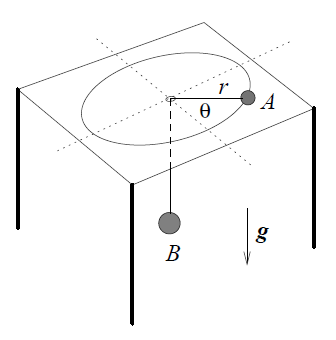
\includegraphics[scale=0.7]{classica-img/mesa.png}
\end{figure}

\resposta



\item Uma partícula de massa $m$ está sujeita ao potencial unidimensional

$$
V(x)=\frac{1}{2} k x^{2}-\frac{k}{4 a^{2}} x^{4}
$$

\begin{figure}[H]
\centering
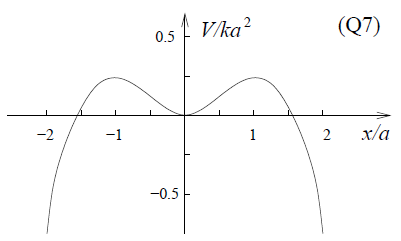
\includegraphics[scale=0.7]{classica-img/pot.png}
\end{figure}
mostrado na figura acima, onde $k$ e $a$ são constantes positivas.


a) Determine a força $F(x)$ e obtenha os pontos de equilíbrio, determinando sua natureza.

\resposta

b) Calcule o período das pequenas oscilações que ocorrem em torno do ponto de equílibrio estável.

\resposta

c) Admita que a partícula esteja em repouso no ponto $x = 0$ e que receba um impulso que lhe confere, instantaneamente, uma velocidade de módulo $v$ na direção de $x$ positivo. Discuta o que ocorre nos seguintes casos: $0<v \leq a \sqrt{k / 2 m} $ e $ v>a \sqrt{k / 2 m}$.

\resposta

d) Esboce o diagrama de fase do sistema ($\dot{x}$ versus $x$ para energia constante) para os diversos tipos de movimento. Indique claramente a curva que corresponde à transição de movimento periódico para não periódico, bem como o valor da energia correspondente.

\resposta




\item Um pêndulo simples é constituído por uma partícula de massa $m$ suspensa por um fio inextensível de comprimento $a$ e massa desprezível. Seu ponto de suspensão é conectado a um suporte que se movimenta horizontalmente sem atrito como mostrado na figura.

\begin{figure}[H]
\centering
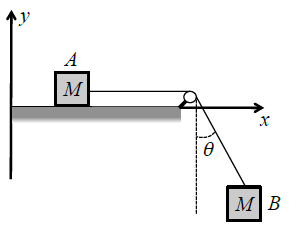
\includegraphics[scale=0.7]{classica-img/pendulo3.png}
\end{figure}

Suponha que o suporte seja muito pequeno e que o pêndulo se movimente apenas no plano vertical. Usando como coordenadas generalizadas $x$ e $\theta$, onde $x$ é a posição horizontal do suporte e $\theta$ o deslocamento angular do pêndulo, conforme se vê na figura, o movimento do sistema é descrito pela lagrangiana:

$$
\mathcal{L}=\frac{m}{2} \dot{x}^{2}+\frac{m}{2}\left(a^{2} \dot{\theta}^{2}+2 a \dot{x} \dot{\theta} \cos \theta\right)+m g a \cos \theta
$$


a) Obtenha a equação de movimento para a coordenada $\theta$.

\resposta

b) Admitindo que os deslocamentos angulares sejam pequenos e que o suporte esteja sujeito a um movimento harmônico forçado de frequência $\omega$, isto é, descrito por $x(t) = x_{0} cos \omega t$, obtenha a solução geral $\theta(t)$ da equação do movimento para a coordenada $\theta$.

\resposta

c) No caso do item anterior, obtenha a frequência de ressonância $\omega R$.

\resposta

d) Escreva a solução geral para $\theta(t)$, quando as condições iniciais forem $\theta(0) = 0$ e $\dot{\theta}(0) = 0$ e o suporte movimentar-se com frequência $\omega < \omega_{R}$.



\item Um átomo de trítio pode ser descrito classicamente como um núcleo com carga elétrica $+e$, composto por um próton e dois nêutrons, circundado por um elétron orbital de carga $-e$, o qual percorre uma órbita circular de raio $r_{0}$. Em um processo conhecido como decaimento beta, o núcleo de trítio se transforma em um núcleo de hélio, composto por dois prótons e um nêutron, emitindo um par de partículas que rapidamente escapa do sistema atômico. Como
consequência desse processo, o átomo de hélio fica ionizado uma vez, e o elétron orbital passa subitamente para uma nova situação, orbitando agora em torno de um núcleo de carga $+2e$.


a) Supondo que o par de partículas que escapa do átomo tenha momento linear total de módulo $p$, obtenha a velocidade de recuo do átomo de hélio de massa $M$.

\resposta

b) Obtenha a energia $E_{a}$ do elétron orbital antes do decaimento beta.

\resposta

c) Calcule a energia $E_{d}$ do elétron orbital depois do decaimento beta e obtenha a razão $\rho = E_{a}/E_{d}$.

\resposta

d) Determine o momento angular total do elétron em função de $r_{0}$ e da massa $m$ do elétron. Calcule a maior e a menor distância entre o elétron e o núcleo na nova órbita em termos de $r_{0}$.

\resposta


\item Um equilibrista de massa $m$ está inicialmente parado na extremidade de uma barra larga, horizontal, homogênea, de comprimento $D$ e massa $M = 3m$. A barra gira em torno de um eixo vertical que passa pelo seu centro. O equilibrista começa então a caminhar sobre a barra, em direção ao eixo de rotação, com velocidade constante. Considere o período inicial de rotação do sistema igual a $T_{0}$.

a) Determine o torque das forças que atuam sobre o equilibrista em relação ao centro da barra.

\resposta

b) Determine o momento angular do sistema quando o equilibrista atinge o centro da barra. Determine o período de rotação do sistema nessa situação.

\resposta

c) Determine as energias nas posições inicial e final do sistema. Nesse movimento, a energia do sistema variou?

Considere o equilibrista como uma massa puntiforme.

Dado: $I_{CM}(barra) = \frac{1}{12} MD^{2}$

\resposta




\item Uma partícula de massa $m$ se encontra no interior de um cano oco, liso, estreito e longo que gira num plano horizontal com velocidade angular $\omega$ constante. O eixo fixo de rotação passa por uma das extremidades do cano, como mostra a figura.

\begin{figure}[H]
\centering
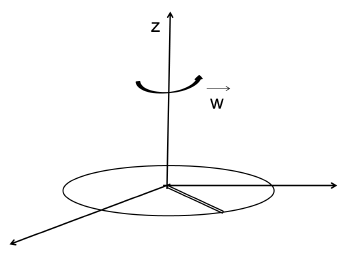
\includegraphics[scale=0.8]{classica-img/angular.png}
\end{figure}


a) Escreva a Lagrangiana da partícula.

\resposta

b) Obtenha as equações de Lagrange do movimento da partícula.

\resposta

c) Determine o movimento da partícula, considerando que inicialmente ela é lançada do centro de rotação com velocidade $\vec{v}_{0}$.

\resposta

d) Obtenha a função Hamiltoniana ($H$) do movimento dessa partícula e as equações de Hamilton do movimento.

\resposta

e) Dentre as grandezas físicas $H$ e $E$ (energia), quais são conservadas? Justifique sua resposta.

\resposta





\item Uma partícula de massa $m$ move-se com velocidade $\vec{v}_{1}$ no semi-plano superior até ser desviada ao atingir o semi-plano inferior, onde passa a se propagar com velocidade $\vec{v}_{2}$, conforme ilustrado na figura abaixo. Observa-se experimentalmente as seguintes características: i) a partícula passa do meio 1 ao meio 2 desde que $v_{1} > v_{min}$; ii) a partícula se move de modo retilíneo e uniforme em cada um dos semi-planos; iii) o ângulo de saída $\theta_{2}$ é diferente do ângulo de entrada $\theta_{1}$, o que nos faz presumir que em cada meio a partícula esteja sob ação de diferentes
potenciais $U_{1}$ e $U_{2}$.

\begin{figure}[H]
\centering
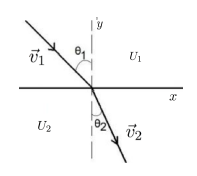
\includegraphics[scale=0.8]{classica-img/refracao.png}
\end{figure}


a) Com base no experimento, esboce o gráfico do potencial $U$ em função de $y$ para $x$ fixo (justificando o gráfico).

\resposta

b) Determine $v_{2}$ em termos de $v_{1}$, de $m$ e dos potenciais $U_{1}$ e $U_{2}$. Qual é a velocidade $v_{min}$ acima da qual observa-se a passagem da partícula do meio 1 para o meio 2?
\item(c) Determine o índice de refração $sen\ \theta_{1} / sen\ \theta_{2}$ em termos de $m$, $v_{1}$ e dos potenciais em cada
meio.

\resposta


\item Uma partícula de massa $m$ desenvolve movimento unidimensional sob ação do potencial abaixo ($c$ é uma constante)

$$
U(x) = \frac{1}{2} x^{4} - c x^{2}.
$$


a) Esboce os gráficos de $U(x)$ e dos respectivos espaços de fase ($\dot{x}$ versus $x$ para todas as energias possíveis) nos seguintes casos : i) $c > 0$, ii) $c = 0$ e iii) $c < 0$.

\resposta

b) Por meio da energia total $E$, identifique todos os movimentos periódicos possíveis e seus respectivos pontos de inversão (onde a velocidade é nula) para cada um dos casos do item (a).

\resposta

c) Determine a dependência do período de oscilações com a energia total $E$ para $c = 0$.

\resposta



\item Duas esferas ocas, ambas de massa $M$ e raio $R$, que estão girando em torno do centro de massa ($CM$) do sistema com um período inicial $T_{0}$, são mantidas distantes $d_{0} = 8R$ uma da outra por um fio ideal que passa pelos respectivos centros, conforme ilustra a figura abaixo.
\begin{figure}[H]
\centering
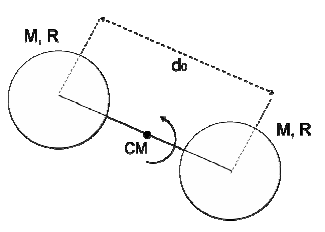
\includegraphics[scale=0.8]{classica-img/rotacional.png}
\end{figure}
Num dado instante um motor, colocado dentro de uma das esferas, começa a enrolar o fio lentamente, aproximando uma esfera da outra. Considere que o momento de inércia do motor seja desprezível quando comparado ao das esferas. Desconsidere efeitos da gravidade e expresse todos os seus resultados em termos de $M$, $R$ e $T_{0}$. Dado: o momento de inércia da casca esférica em relação a um eixo que passa pelo seu centro é $\frac{2}{3} MR^{2}$.

a) Determine o momento angular desse sistema em relação ao seu centro de massa, antes do motor ser ligado.

\resposta

b) Calcule a velocidade angular de rotação, $\omega_{f}$ , no instante em que uma esfera encosta-se à outra.

\resposta

c) Calcule a variação da energia cinética do sistema até esse instante.

\resposta

d) Qual foi o trabalho realizado pelo motor para fazer com que as esferas se encostem?

\resposta


\item Um pêndulo simples consiste de uma massa m pendurada a partir de um ponto fixo por uma barra estreita de massa desprezível, inextensível, de comprimento $\ell$. Seja $g$ a aceleração da gravidade local e $\theta$ o ângulo entre o pêndulo e a direção vertical. No que segue, faça sempre a aproximação de pequenos ângulos.

a) Escreva a equação de movimento desprezando o atrito. Obtenha a frequência natural $\omega$ do pêndulo.

\resposta

b) Determine $\theta(t)$ para as seguintes condições iniciais: $\theta(0)=0$ e $\frac{d \theta}{d t}(0)=\Omega$.

\resposta

c) Escreva a equação do movimento do pêndulo na presença de uma força de atrito viscoso dada por $F_{R}=2 m \sqrt{g l} \frac{d \theta}{d t}$.

\resposta

d) Na situação do item (c), determine $\theta (t)$ para as seguintes condições iniciais: $\theta(0) = \theta_{0}$ e $\frac{d\theta}{dt} (0) = 0$.

\resposta


\item Um corpo celeste de massa $m$ se aproxima do Sol (massa $M >> m$) seguindo uma trajetória hiperbólica e quando está a uma distância $r_{0}$ dele, a sua velocidade é $v_{0}$ e faz um ângulo de $30º$ com o raio vetor ao Sol.

a) Calcule o momento angular $L$ e a energia $E$ desse corpo celeste.

\resposta

b) Determine a distância $r_{p}$ de máxima aproximação do corpo celeste ao Sol, expressando o seu resultado em termos de $L$ e $E$.

\resposta

c) Quando o corpo celeste atinge a distância $r_{p}$ de máxima aproximação, sofre um choque com um pequeno asteróide de tal maneira que sua massa não varia, porém ele passa a descrever órbita circular de raio $r_{p}$ no mesmo plano da órbita anterior. Calcule a nova energia e o novo momento angular do corpo celeste após a colisão, expressando o seu resultado em termos de $r_{p}$.

\resposta


\item Uma bola de massa $m = 450 g$ está presa a uma mola cuja energia potencial em função da elongação $x$ está mostrada na figura abaixo (linha sólida). Expresse as respostas no SI.

a) Determine a constante elástica da mola, para pequenos deslocamentos.

\resposta

b) Esboce um gráfico da força que atua sobre essa bola em função da elongação da mola. Sabendo que o movimento da bola é unidimensional e sua elongação máxima é de 3 $cm$:

\resposta

c) determine sua velocidade máxima;

\resposta

d) determine a energia cinética da bola nesse movimento para a elongação da mola $x = - 2 cm$;

\resposta

e) Determine a posição ($x < 0$) em que a bola deve ser solta a partir do repouso para atingir o ponto $x = 5 \ cm$ com velocidade nula.

\begin{figure}[H]
\centering
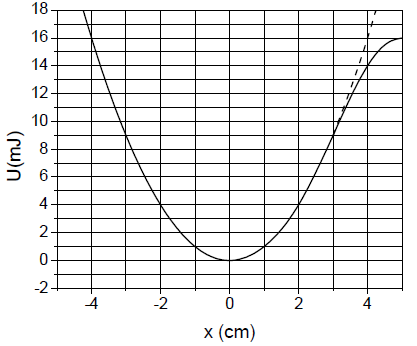
\includegraphics[scale=0.8]{classica-img/grafico.png}
\end{figure}

\resposta

\item Considere um corpo de massa $M$ de seção transversal circular de raio $R$ que rola sem deslizamento sobre um plano que possui um ângulo de inclinação $\mu$ em relação à horizontal, conforme mostra a figura abaixo. O coeficiente de atrito estático entre o corpo e o plano é $\mu_{e}$. O momento
de inércia do corpo em relação a um eixo passando pelo ponto $O$ é $I$ e a aceleração da gravidade é $g$.


a) Desenhe o diagrama de forças para o corpo. Escreva a equação que relaciona a velocidade angular, $\dot{\phi}$, de rolamento do corpo e a velocidade de translação, $\dot{x}$, que caracteriza um rolamento sem deslizamento.

\resposta

b) Determine a aceleração $\ddot{x}$, associada à translação do corpo ao longo do plano inclinado, em termos dos parâmetros que constam no enunciado.

\resposta

c) Assuma que o corpo inicia o seu movimento a partir do repouso na origem do sistema de coordenadas cartesianas indicado na figura. Calcule a energia mecânica no início e no final do movimento. A energia mecânica do sistema é conservada?

\resposta

d) Calcule o momento de inércia $I$ considerando que o corpo seja (i) um anel e (ii) um disco. Assuma que as massas dos corpos estão uniformemente distribuídas. Suponha agora que o ângulo $\mu$ possa ser variado. A partir de qual $\mu$ cessa o movimento de rolamento puro e o corpo começa a deslizar, nos casos (i) e (ii) acima? Deixe a resposta em termos de $\mu_{e}$.

\resposta


\item Considere o pêndulo invertido da figura abaixo, composto por uma barra de massa M e momento de inércia $I_{0}$ em relação ao seu centro de massa, cujas coordenadas são ($X,Y$). A barra pode girar livremente no plano $xy$ em torno de um eixo de rotação que passa pela posição ($x_{p},y_{p}$), a uma distância $\ell$ do centro de massa. A aceleração da gravidade é $g$.
\begin{figure}[H]
\centering
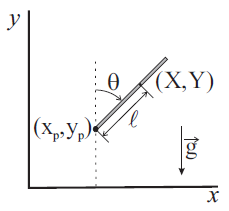
\includegraphics[scale=0.8]{classica-img/pendulo5.png}
\end{figure}

a) Escreva as equações para a energia cinética e potencial do sistema em termos de $X$, $Y$ e $\mu$. Para os itens (b), (c) e (d) assuma que um agente externo faz o eixo de rotação oscilar horizontalmente com frequência angular $\omega$, ou seja, tem-se $y_{p}(t) = 0$ e $x_{p}(t) = A cos(\omega t)$.

\resposta

b) Escreva a lagrangiana do sistema em termos da coordenada generalizada $\theta$.

\resposta

c) Escreva a equação de movimento para a lagrangiana do item (b).

\resposta

d) Considere que o sistema executa pequenas oscilações ($\theta$ pequeno). Mostre que neste caso, $\theta(t) = \alpha cos(\omega t) + \beta sen( \omega t)$ é uma solução para o problema. Determine $\alpha$ e $\beta$.

\resposta


\item Uma bala de massa $m$ é disparada com velocidade $v$ contra um disco homogêneo de massa $M$ e raio $R$, inicialmente parado, que se encontra deitado sobre uma superfície horizontal lisa sem atrito. Suponha que a bala atinja o disco como indicado na figura e fique retida na superfície do disco. Considere que o centro de massa do sistema (disco + bala) após a colisão coincide com o centro do disco. $Dado$: $I_{disco}^{CM} = \frac{1}{2} M R^{2}$.

a) Qual é a velocidade do centro do disco após a colisão?

\resposta

b) Qual é a velocidade angular dos sistema (disco + bala) após a colisão?

\resposta

c) Qual é a variação de energia dos sistema devido à colisão?

\begin{figure}[H]
\centering
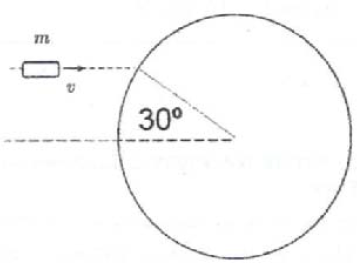
\includegraphics[scale=0.7]{classica-img/angular2.png}
\end{figure}

\resposta

\item Uma partícula de massa $m$ sob a ação da gravidade $g$ constante está vinculada a se mover no interior da superfície de um cone invertido cuja geratriz forma um ângulo $\alpha$ com o eixo do cone. O vértice do cone está na origem e seu eixo ao longo da direção vertical. O atrito pode ser desprezado.

a) Determine a energia cinética e a energia potencial da partícula. \textit{Sugestão: utilize coordenadas esféricas.}

\resposta

b) Escreva a lagrangiana do sistema e obtenha as equações do movimento.

\resposta

c) Há grandezas físicas conservadas no movimento dessa partícula? Se há, diga quais são essas grandezas, argumentando sobre como chegou à conclusão de que são conservadas.

\resposta

d) A partir da definição da hamiltoniana, obtenha sua forma explícita em termos das coordenadas e momentos generalizados, e compare-a com a energia mecânica da partícula.

\resposta

e) Mostre que a partícula, em questão pode executar pequenas oscilações radiais em torno de um raio de equilíbrio $r_{0}$ e determine sua frequência. Compare o valor obtido com a frequência de revolução no movimento circular.

\resposta


\item Uma partícula de massa $m$ colide com uma barra fina e homogênea inicialmente em repouso, de momento de inércia $I = Ml^{2}/12$ relativo ao seu centro de massa, sendo $M$ a sua massa e $\ell$ o seu comprimento. Antes da colisão, a partícula move-se perpendicularmente à barra com velocidade $v_{0}$. A partícula colide elasticamente com a extremidade da barra, conforme ilustra a figura a baixo.
\begin{figure}[H]
\centering
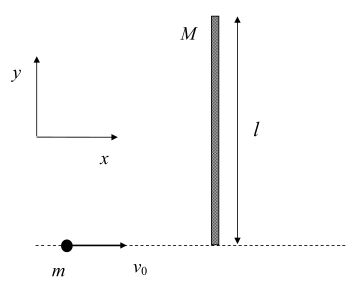
\includegraphics[scale=0.7]{classica-img/colide.png}
\end{figure}

a) Escreva as equações que expressam as grandezas físicas conservadas na colisão.

\resposta

b) Determine o vetor velocidade de translação do centro de massa da barra imediatamente após a colisão.

\resposta

c) Determine o vetor velocidade angular de rotação da barra imediatamente após a colisão.

\resposta

d) Determine o vetor velocidade da partícula imediatamente após a colisão.

\resposta


\item Uma partícula de massa $m$ pode se mover sem atrito num aro de raio $R$, como mostrado na figura abaixo. O aro gira com velocidade angular constante $\omega$ em torno do eixo vertical, como mostra a figura abaixo. Considere a aceleração da gravidade $g$.
\begin{figure}[H]
\centering
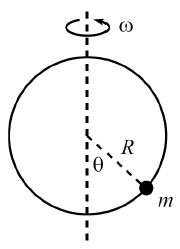
\includegraphics[scale=0.7]{classica-img/particula2.png}
\end{figure}

a) Determine a energia cinética da partícula em função de $\theta$, $\dot{\theta}$, $R$, $m$, e $\omega$.

\resposta

b) Determine a lagrangiana da partícula, adotando energia potencial nula no ponto correspondente a $\theta = 0$.

\resposta

c) Determine a equação de movimento da partícula.

\resposta

d) Determine os pontos de equilíbrio.

\resposta


\item A interação entre dois átomos de massas $m_{1}$ e $m_{2}$, que formam uma molécula, pode ser descrita pelo potencial de Lennard-Jones dado por
$$
V(x) = A \left[ \left( \frac{b}{x} \right)^{12} - 2 \left( \frac{b}{x} \right)^{6} \right]
$$
onde $A$ e $b$ são parâmetros positivos e $x$ a separação interatômica. Trate o problema classicamente e despreze qualquer tipo de rotação da molécula.

a) Determine a posição de equilíbrio em função de $A$ e $b$.

\resposta

b) Calcule a menor energia para dissociar a molécula.

\resposta

c) Mostre que o equilíbrio é estável e calcule a frequência de pequenas oscilações em torno da posição de equilíbrio.

\resposta

d) Desenhe um gráfico do potencial de Lenard-Jones indicando os parâmetros obtidos nos itens (a) e (b).

\resposta


\item Atualmente, a totalidade dos atletas de alto nível de salto em altura utiliza uma técnica para o salto batizada de "Salto Fosbury". Suponha que nesse salto o atleta possa ser aproximado por uma barra rígida de comprimento $\ell$, inclinada por um ângulo $\theta$ e movendo-se com uma velocidade $v_{0}$ para a direita conforme mostra a figura abaixo. No momento do "salto" essa barra começa a girar em torno do ponto \textbf{P}. A barra possui uma massa $m$ homogeneamente distribuída.
\begin{figure}[H]
\centering
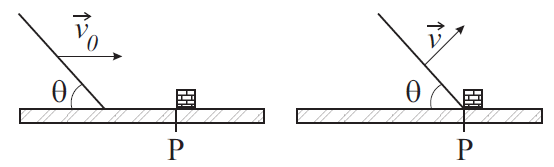
\includegraphics[scale=0.7]{classica-img/massa.png}
\end{figure}

a) Calcule o momento de inércia da barra em relação à sua extremidade.

\resposta

b) A conservação de uma grandeza física permite que a barra obtenha uma componente vertical para a velocidade do seu centro de massa. Qual é essa grandeza física?

\resposta

c) Calcule a componente vertical $\nu_{v}$ da velocidade do seu centro de massa imediatemente após atingir o ponto \textbf{P}.

\resposta

d) Qual é a altura máxima atingida pelo seu centro de massa em relação ao solo.

\resposta


\item Uma barra uniforme de comprimento $L$ e massa $M$ está em equilíbrio numa mesa horizontal sobre a qual pode mover-se sem atrito. Num dado instante a barra recebe um impulso, $J$, de curta duração perpendicular à barra num ponto P da barra tal que $OP = r$, onde  $O$ é o centro de massa da barra.

a) Logo após o impulso, qual é a velocidade do centro de massa da barra?

\resposta

b) Qual é a velocidade angular da barra em torno do centro de massa?

\resposta

c) Qual é a velocidade da extremidade da barra mais afastada do ponto de impacto P?

\resposta

d) Qual é a localização de um ponto $Q$ da barra, para o qual a velocidade instantânea é nula?

\resposta



\item Uma maneira de transferir um foguete de uma órbita circular para outra é fazê-lo percorrer uma órbita elíptica de transferência que tangencia as duas órbitas circulares. Considere que as órbitas da Terra e de Marte são órbitas circulares de raios iguais à $R_{1}$ e $R_{2}$ respectivamente e que um foguete é lançado da Terra até Marte numa órbita elíptica de transferência tal que o seu periélio (distância de maior aproximação) está na órbita de Terra e o seu afélio (distância de maior afastamento) na órbita de Marte.

a) Qual é a velocidade do foguete relativa a Marte quando eles se encontram?

\resposta

b) O que devemos fazer para que o foguete pouse em Marte?

\resposta

c) Qual é o tempo de transferência?

\item[] São conhecidos: $G$: (constante gravitacional) e $M$ (massa do sol).

\resposta

\item Dois patinadores de mesma massa estão sobre a superfície de um lago congelado. Um deles, A, está em repouso, enquanto que o outro, B, se aproxima do primeiro com velocidade $\vec{v}$ e parâmetro de impacto $b$ menor que o comprimento dos braços dos patinadores. No instante em que a distância entre eles é mínima, eles seguram-se pelas mãos.

a) Qual é a velocidade angular de rotação dos patinadores em torno do centro de massa?

\resposta

b) Qual é o tempo mínimo que eles devem permanecer unidos para que o patinador que estava parado, A, saia formando um ângulo de $30°$ com a direção de $\vec{v}$ no sistema de laboratório?

\resposta

c) Qual é a tensão nos braços dos patinadores?

\resposta


\item Duas partículas de massas iguais a $m$ estão ligadas por uma corda inextensível de comprimento $\ell$ e massa desprezível, que passa por um pequeno furo sobre uma mesa horizontal. Uma das partículas se move na superfície da mesa horizontal e a outra ao longo da direção vertical.

a) Tomando para coordenadas generalizadas, as coordenadas polares $\rho$, $\phi$ da partícula que se move no plano da mesa, num sistema de coordenadas cuja origem coincide com o furo na mesa, mostre que a lagrangeana do sistema é igual a:
$$
L = m\dot{\rho}^{2} + \frac{1}{2} m \rho^{2} \dot{\rho}^{2} - mg\rho
$$

\resposta

b) Escreva as equações de Lagrange.

\resposta

c) Mostre que o momento angular em relação do furo da mesa é uma constante do movimento.

\resposta

d) Mostre que é possível haver movimento circular no plano da mesa.
\item[] Calcule o momento angular e a energia do sistema, se a partícula no plano da mesa se move numa órbita circular de raio R.

\resposta


\item Uma partícula de massa $m$ e carga $q$ é lançada verticalmente da superfície terrestre com velocidade $v_{0}$ na direção de uma carga $Q$ de sinal oposto ao da carga $q$, Qq<0, fixa a uma altura h suficientemente pequena para considerarmos $g$ constante. A energia potencial da partícula é igual a, para $0 < z < h$:
$$
U(z) = mgz - \frac{|Qq|}{h-z}
$$

a) Mostre que se $h$ é menor que um valor mínimo $h_{min}$, as cargas sempre se chocam, independente do valor de $v_{0}$.

\resposta

b) Mostre que se $h$ exceder esse valor, as cargas se chocam somente se $v_{0}$ for maior do que um valor mínimo, $v_{min}$.

\resposta

c) Nas condições do item (b), existe um ponto de equilíbrio? Ele é estável?

\resposta


\item O ponto de suspensão de um pêndulo de massa $m$ e comprimento $\ell$ oscila na direção horizontal de acordo com a equação
$$
x_{p} = a \operatorname{cos} \omega t
$$
Considere que o pêndulo se move num plano vertical.

a) Mostre que a lagrangeana do sistema é igual a:
$$
L = \frac{m}{2} (\dot{x}_{p}^{2} + \ell^{2} \dot{\theta}^{2} + 2 \ell \operatorname{cos}(\theta) \dot{x}_{p} \dot{\theta} ) + mgl \operatorname{cos} \theta
$$
onde $\theta$ é o ângulo que a direção do pêndulo faz com a vertical.

\resposta

b) Escreva a equação de Lagrange.

\resposta

c) Interprete a equação de movimento deduzida no item (b) do ponto de vista de um observador fixo no ponto de suspensão do pêndulo. Qual é a origem dos termos desta equação?

\resposta


\item Duas estrelas, de massas $m_{1}$ e $m_{2}$, se movem em órbitas circulares em torno do seu centro de massa, sob a ação da atração gravitacional entre ambas. O centro de massa está em repouso e a distância entre elas é igual a $D$.

a) Calcule os raios das órbitas circulares.

\resposta

b) Faça um gráfico das órbitas. Assinale uma possível posição das estrelas, num dado instante $t$. Considere $m_{1} >  m_{2}$.

\resposta

c) Qual é o período do movimento orbital?

\resposta

d) Que observação astronômica indicaria que um dos constituintes desse sistema binário seja um buraco negro?

\resposta


\item Um astronauta está viajando numa nave que é um disco de massa M e raio R. Por engano ele aciona dois foguetes, que são lançados ao mesmo tempo, tangentes à nave e em direções opostas, com velocidade $v$ e massas $m$. Os pontos de lançamento são diametralmente opostos e a nave inicialmente estava em repouso. Considere $M >> m$.

a) Qual a velocidade angular da nave após o lançamento?

\resposta

b) Que propriedade você usou para responder à pergunta do item $a$?

\resposta

c) O astronauta, para interromper a rotação da nave, lança um jato de combustível de massa igual a $\frac{m}{10}$, tangente à nave. Qual deve ser a velocidade de lançamento?

\resposta

d) Após o lançamento do combustível, a nave fica estacionária? Explique.
\item[] Dado: Momento de inércia do disco em torno do eixo de simetria, perpendicular ao plano do disco, $I = \frac{MR^{2}}{2}$.

\resposta


\item Uma nave espacial tem a forma de um cilindro oco de raio interno $R_{1}$ e raio externo $R_{2}$. A região compreendida entre os raios $R_{1}$ e $R_{2}$ é a região oca, sendo o "teto" da nave a superfície de raio $R_{1}$ e o "solo" a de raio $R_{2}$. A nave está numa região livre de campos gravitacionais, mas o efeito da gravidade pode ser simulado fazendo com que a nave gire com velocidade angular $\omega$ em torno do eixo de simetria do cilindro.

a) Se um objeto de massa $m$ está preso no teto da nave, qual é o seu "peso"?

\resposta

b) Se deixarmos o objeto cair , quais são suas trajetórias, vistas por: um observador  num referencial inercial e um observador num referencial fixo na nave? Responda sem fazer cálculos.

\resposta

c) Quanto tempo ele leva para atingir o "solo"?

\item[] Dados:
\item[] Força centrífuga$ = - m \vec{\omega} \times (\vec{\omega} \times \vec{r})$
\item[] Força de Coriolis$ = -2m (\vec{\omega} \times \vec{v})$

\resposta


\item Uma partícula de massa $m$ se move na superfície de um cilindro de raio $R$ sob a ação da gravidade e de uma força central cuja energia potencial é
$$
U_{cent} = \frac{kr^{2}}{2},
$$
onde $r$ é a distância da partícula ao centro de forças e $k$ é uma constante positiva. O centro de forças está localizado no eixo de simetria do cilindro e esse eixo de simetria está na direção vertical (ver figura abaixo; a aceleração da gravidade tem sentido oposto a $Oz$).
\begin{figure}[H]
\centering
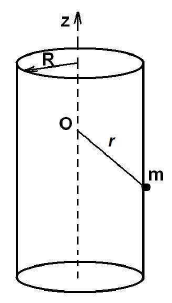
\includegraphics[scale=0.7]{classica-img/cilindro.png}
\end{figure}


a) Mostre que a lagrangeana da partícula em coordenadas cilíndricas num sistema de coordenadas com origem no centro de forças e eixo $Oz$ na direção vertical é dada por:
$$
L  = \frac{m}{2} (R^{2} \dot{\phi}^{2} + \dot{z}^{2} ) - mgz - \frac{k}{2} (z^{2} + R^{2}).
$$

\resposta

b) Escreva as equações de Lagrange.

\resposta

c) É possível haver movimento circular em um plano horizontal? No caso afirmativo, qual é a localização do plano?

\resposta

d) Determine a frequência de pequenas oscilações em torno do movimento circular.

\resposta



\item Decidiu-se colocar em órbita um satélite geoestacionário em duas etapas. Inicialmente o satélite se encontra numa órbita circular de estacionamento, no mesmo plano da órbita geoestacionária. O período da órbita de estacionamento é igual a $\frac{2}{3}T$, onde $T$ é o período de rotação da Terra em torno do seu eixo. Para transferir o satélite para a órbita circular geoestacionária foi decidido fazê-lo através de uma órbita elíptica cujo perigeu (distância de maior aproximação) está na órbita de estacionamento e o apogeu (distância de maior afastamento) na órbita geoestacionária.

a) Qual é a localização do plano das órbitas satélite?

\resposta

b) Determine, em função dos dados abaixo, os raios das órbitas de estacionamento e geoestacionária.

\resposta

c) Qual é o tempo de transferência?

\resposta

d) Discuta como se deve proceder para que o satélite se encontre, no fim da operação, sobre o mediano de Brasília.

\item[] Dados:
\item[] $G =$ constante gravitacional.
\item[] $M =$ massa da Terra.
\item[] $T =$ período de rotação da Terra em torno do seu eixo.
\item[] \textbf{Observação: fornecer as respostas em função dos dados.}

\resposta



\item Um cubo uniforme de aresta $2a$ e massa $M$ desliza com velocidade $v$ sobre uma mesa horizontal quando se choca com uma saliência da mesa, paralela à aresta do cubo, e gruda na saliência, passando a rodar em torno dela.

a) Qual é a velocidade angular do cubo devida ao choque?

\resposta

b) Qual é a perda de energia cinética imediatamente após o choque?

\resposta

c) Determine o valor mínimo de $v$ para que o cubo tombe (caia do outro lado da saliência.)

\item[] Dado:
\item[] Tensor de inércia do cubo num sistema de coordenadas cujo eixo $Oz$ coincide com uma das arestas e a origem está no meio da aresta:

$$
I = \left(
\begin{array}{ccc}
\frac{5}{3} M a^{2} & -Ma^{2} & 0 \\
- M a^{2} & \frac{5}{3} M a^{2} & 0 \\
0 & 0 & \frac{5}{3} M a^{2} \\
\end{array}
\right)
$$



\item Um objeto de massa $M_{1}$ está preso no teto de um elevador de massa $M_{2}$. O elevador está see deslocando para cima pela ação de uma força constante $F$, $F > (M_{1} + M_{2})g$. O objeto de massa $M_{1}$ está preso no teto através de um fio inextensível e está a uma distância $s$ do chão do elevador.

a) Qual é a aceleração do elevador?

\resposta

b) Qual é a tensão no fio inextensível?

\resposta

c) Se o fio quebra repentinamente, qual é a aceleração do elevador? Qual é a aceleração do objeto de massa $M_{1}$?

\resposta

d) Quanto tempo leva para o objeto de massa $M_{1}$ atingir o chão do elevador?

\item[] Dados: $F$, $M_{1}$, $M_{2}$, $g$, $s$.
\item[] Observação: fornecer as respostas em função dos dados.




\item Uma partícula e uma barra podem se mover livremente sobre a superfície lisa de uma mesa horizontal. A barra tem comprimento $D$ e massa igual à massa da partícula, $M$. Inicialmente a barra está em repouso, e a partícula se move com velocidade $v$ perpendicular à barra. Suponha que a partícula colide com a barra e que a colisão é elástica.

a) Descreva os movimentos subsequentes da partícula e da barra quando a partícula colide com a barra no seu centro de massa (ver figura a) abaixo).

\resposta

b) Descreva os movimentos subsequentes da partícula e da barra quando a partícula colide com a barra numa das suas extremidades (ver figura b) abaixo).

\resposta

c) No caso do item (b), determine as velocidades da partícula, $v_{p}$, da barra, $v_{b}$, e a velocidade angular de rotação da barra em torno do seu centro de massa, $w$.

\item[] Momento de inércia da barra relativo a um eixo passando pelo centro de massa e perpendicular à barra: $I = MD^{2}/12$.

\begin{figure}[H]
\centering
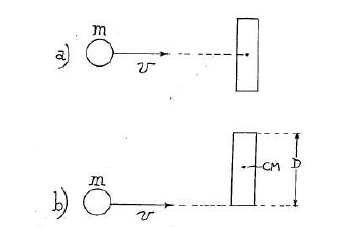
\includegraphics[scale=0.7]{classica-img/barra2.png}
\end{figure}

\resposta


\item Um objeto de massa $m$ desliza num trilho liso mostrado na figura ao lado. Inicialmente o objeto está em repouso, a uma altura $h$ acima do topo do semicírculo $AC$.
\begin{figure}[H]
\centering
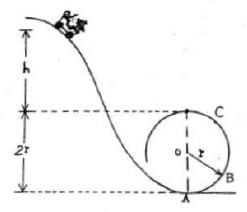
\includegraphics[scale=0.7]{classica-img/trilho.png}
\end{figure}

a) Faça um diagrama das forças que agem no objeto quando ele está no ponto $B$ do semi-círculo. Defina $\theta$ como o ângulo do vetor posição medido em relação à direção $\overline{OA}$. Escreva as equações de movimento nas direções radial e tangencial.

\resposta

b) Qual é a magnitude e direção da força exercida no objeto pelo trilho, quando ele passa no ponto A?

\resposta

c) Mostre que $h \geq r/2$, para que o objeto atinja o ponto C do trilho.

\resposta

d) Para $h < r/2$ o objeto abandona o trilho antes de atingir o ponto C. Mostre que isto ocorre na posição tal que $-3 \operatorname{cos} \theta = 2 + 2h/r$.

\resposta




\item Um plano inclinado de um ângulo $\alpha$ é acelerado horizontalmente. A magnitude da aceleração aumenta gradualmente até que um bloco de massa $m$, originalmente em equilíbrio com respeito ao plano inclinado, começa a subir no plano. O coeficiente de atrito estático entre o bloco e o plano é $\mu = 5/4$.

a) Desenhe um diagrama mostrando as forças que atuam no bloco, pouco antes dele subir no plano, visto de um referencial inercial.

\resposta

b) Ache a aceleração do plano quando o bloco começa a subir.

\resposta

c) Repita o item (a) visto de um referencial não inercial, fixo no plano.
\item[] Dado: $\operatorname{cos} \alpha = 0,8$; $\operatorname{sen} \alpha = 0,6$

\resposta



\item Uma partícula de massa igual a $m$ se move no interior de um cano liso. O cano, por sua vez, gira num plano horizontal com velocidade angular $\omega$ constante em torno de um ponto fixo no cano.

a) Quantos graus de liberdade tem a partícula?

\resposta

b) Considere como coordenada generalizada a posição da partícula ao longo do cano, $s$, com a origem no centro de rotação. Mostre que a lagrangeana do sistema é dada por:
$$
L = \frac{1}{2} m \left( \dot{s}^{2} + \omega^{2} s^{2} \right)
$$

\resposta

c) Escreva a equação de Lagrange. Existe um ponto de equilíbrio? Ele é estável?
d) Determine a força de reação do cano. Do ponto de vista de um observador fixo no cano, qual é a origem da força de reação?

\resposta




\item A massa $m$ de um pêndulo está presa por um fio ideal de comprimento $\ell$ a um ponto de sustentação. Esse ponto se move para a frente e para trás ao longo de um eixo horizontal, de acordo com a equação $x = a \operatorname{cos} \omega t$. Suponha que o pêndulo só oscile no plano vertical que contém o eixo $x$. Considere que a posição do pêndulo seja descrita por um ângulo $\theta$ que o fio faz com uma linha vertical.

a) Escreva a Lagrangeana e obtenha as equações de Lagrange.

\resposta

b) Mostre que, para valores pequenos de $\theta$, a equação de movimento se reduz à equação de movimento de um oscilador harmônico forçado.

\resposta

c) Determine o movimento para o estado estacionário correspondente ao ítem (b) encontrando a amplitude de oscilações do estado estacionário.

\resposta


\item Uma partícula de massa $m$ se move num poço de potencial $U(x) = a \operatorname{ln}(x) + b/x^{2}$, onde $x$ é a distância da partícula ao centro de forças e $a$ e $b$ são constantes positivas. Considere apenas $x > 0$.

a) Qual a força que age sobre a partícula? Esboce os gráficos de $F(x)$ e de $U(x)$.

\resposta

b) Quais os pontos de equilíbrio e quais as características desses pontos? Quais os possíveis movimentos da partícula?

\resposta

c) Se houver pontos de equilíbrio estável, calcule o período de pequenas oscilações em torno desses pontos.

\resposta


\item Um cometa de massa $m$ descreve uma órbita hiperbólica em torno do Sol (massa $M$) e quando está a uma distância $r_{0}$ se aproximando do Sol, a sua velocidade é $v_{0}$ e faz um ângulo de $30º$ com o raio vetor ao Sol.

a) Calcule o momento angular e a energia desse cometa.

\resposta

b) Determine a distância $r_{p}$ de máxima aproximação do cometa ao Sol.

\resposta

c) Quando o cometa atinge a distância $r_{p}$ de máxima aproximação, sofre um choque com um pequeno asteróide de tal maneira que sua massa não varia porém ele passa a descrever órbita circular de raio $r_{p}$ no mesmo plano da órbita anterior. Calcule a nova energia e o novo momento angular após a colisão.

\resposta



\item Considere uma partícula de massa $m$ movendo-se sob a ação do potencial $V (x) = k x^{2}/2 - kx^{4}/(4a^{2})$ onde $k$ e $a$ são constantes positivas. Suponha que o movimento seja unidimensional e despreze as forças de atrito.

a) Escreva a equação de movimento.

\resposta

b) Faça um esboço do gráfico de $V (x)$ e descreva os tipos de movimentos possíveis.

\resposta

c) Mostre que a função $h(x, \dot{x}) = m\dot{x}^{2} / 2 + V (x)$ é uma constante do movimento.

\resposta

d) Encontre a solução $x(t)$ para o caso $h = k a^{2} / 4$ e $x(0) = 0$.

\resposta



\item Considere um pêndulo plano formado for uma haste inextensível de comprimento $l$ e massa desprezível tendo na sua extremidade uma partícula pontual de massa $m$.

a) Escreva as equações de movimento da partícula em coordenadas polares $r$ e $\theta$.

\resposta

\begin{figure}[H]
\centering
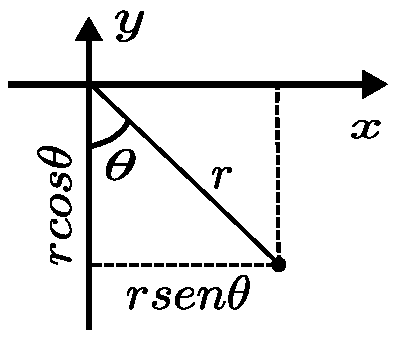
\includegraphics[scale=0.4]{classica-img/pendulo1.pdf}
\end{figure}

Da figura a cima  extrai-se as coordenadas polares. E suas derivadas são:
$$
\begin{array}{ccccccc}
x & = & r \mathrm{sen} \theta & \Rightarrow & \dot{x} & = & \dot{r} \mathrm{sen} \theta + r \dot{\theta} \mathrm{cos} \theta \\
y & = & r \mathrm{cos} \theta & \Rightarrow & \dot{y} & = & \dot{r} \mathrm{cos} \theta - r \dot{\theta} \mathrm{sen} \theta
\end{array}
$$

Da energia cinética e potencial
$$
T = \frac{1}{2}m (\dot{x}^{2} + \dot{y}^{2}) = \frac{1}{2}m ( \dot{r}^{2} + r^{2} \dot{\theta}^{2} ), \ \ \
V = m(-g)y = - mgr \mathrm{cos}\theta
$$
%
Temos que a lagrangeana em coordenadas polares planas
%
$$
L = T - V = \frac{1}{2} m ( \dot{r}^{2} + r^{2} \dot{\theta}^{2} ) + mgr \mathrm{cos}\theta
$$
%
Das equações de movimento
%
$$
\frac{d}{dt} \left( \frac{\partial L }{ \partial \dot{r} }  \right) - \frac{ \partial L }{\partial r} = 0, \quad \quad
\frac{d}{dt} \left( \frac{\partial L }{ \partial \dot{\theta} }  \right) - \frac{ \partial L }{\partial \theta} = 0
$$
Fazendo as derivadas:
$$
\frac{d}{dt} \left( \frac{\partial L }{ \partial \dot{r} }  \right) = \frac{d}{d t} (m \dot{r}) = m \ddot{r}; \quad \quad
\frac{\partial L}{\partial r} = mr \dot{\theta}^{2} + mg \mathrm{cos}\theta
$$
Temos a equação de movimento em relação a $r$:
$$
m \ddot{r} - mr \dot{\theta}^{2} - mg\mathrm{cos} \theta = 0 \Rightarrow \boxed{\ddot{r} - r \dot{\theta}^{2} - g \mathrm{cos}\theta  = 0}
$$
E como:
$$
\frac{d}{dt} \left( \frac{\partial L}{\partial \dot{\theta} } \right) = \frac{d}{dt} (mr^{2} \dot{\theta})  = mr^{2} \ddot{\theta} + 2mr \dot{r} \dot{\theta}; \quad \quad \frac{\partial L}{\partial \theta} = - mgr \operatorname{sen}\theta
$$
Temos a equação de movimento em relação a $\theta$:
$$
mr^{2} \ddot{\theta} + 2mr \dot{r} \dot{\theta} + mgr \operatorname{sen} \theta = 0 \Rightarrow \quad  \boxed{ r^{2} \ddot{\theta} + 2r\dot{r} \dot{\theta} + gr \operatorname{sen} \theta = 0}
$$




b) Suponha que o pêndulo seja lançado de $\theta(0) = \theta_{0}$ com $\dot{\theta}_{0} = 0$. Calcule o valor máximo que a tensão na haste atinge durante o movimento.

\resposta Então, o pêndulo é solto em um ângulo inicial $\theta_{0}$ com velocidade angular $\dot{\theta}_{0} = 0$. Quando passa pelo ponto de equilíbrio a tensão na haste é máxima:
$$
T = F_{p} + F_{c} \Rightarrow mg + m\ddot{\theta} = mg + m \left( - \frac{g}{l} sen \theta_{0}  \right) = mg \left( 1 - \frac{1}{l} sen \theta_{0} \right)
$$



c) Encontre $\theta(t)$ na aproximação de pequenas oscilações supondo $\theta(0) = \theta_{0}$ e $\dot{\theta}_{0} = 0$.

\resposta Utilizando os vínculos ( $r = l$, $\dot{r} = 0$ ) nas equações de movimento, vemos que uma delas se torna familiar no caso de pequenas oscilações:
$$
r^{2} \ddot{\theta} + 2r\dot{r} \dot{\theta} + gr \operatorname{sen} \theta = 0 \Rightarrow \quad l^{2} \ddot{\theta} + gl \operatorname{sen} \theta = 0 \Rightarrow \quad \ddot{\theta} + \frac{g}{l} \operatorname{sen} \theta = 0
$$
Para $\theta << 1$ vale a aproximação:
$$
\mathrm{sen}(\theta) = \sum_{n=0}^{\infty} \frac{\theta^{2n + 1}}{(2n+1)!} = \theta + \frac{\theta^{3}}{3!} + \frac{\theta^{5}}{5!} + (...) \approx \theta
$$
Logo:
$$
\ddot{\theta} + \frac{g}{l}\mathrm{sen} \theta  = 0 \Rightarrow \ddot{\theta} + \frac{g}{l} \theta =  \ddot{\theta} + \omega^{2} \theta = 0
$$
Que é a equação do oscilador harmônico, cuja freqüência é dada por: $\omega = \sqrt{\frac{g}{l}} $. E solução geral é dada por
$$
\theta (t) = A \mathrm{cos} (\omega t + \varphi)
$$
Com $A$ e $\varphi$ constantes fixadas pelas condições iniciais. Para demonstrar que esta é a solução, basta testarmos:
$$
\begin{array}{ccc}
  \ddot{\theta} + \omega^{2} \theta & = & \frac{d^{2}}{dt^{2}} A \mathrm{cos}(\omega t + \varphi) + \omega^{2} A \mathrm{cos}(\omega t + \varphi)   \\
   & = & - \omega \frac{d}{dt} A \mathrm{sen} (\omega t + \phi) + \omega^{2} A \mathrm{cos}(\omega t + \varphi) \\
   & = & - A \omega^{2} \mathrm{cos} (\omega t + \varphi) + \omega^{2} A \mathrm{cos} (\omega t + \varphi) = 0
\end{array}
$$
Portanto a função dada é solução da equação acima. Quanto às constantes, fixemo-las a partir das condições iniciais e tomando $0 \leq \varphi < 2\pi $
%
$$
\begin{array}{ccc}
\theta(0) & = & A \mathrm{cos} \varphi  =  \theta_{0} \Rightarrow A = \frac{\theta_{0}}{\mathrm{cos} \varphi}; \\
\dot{\theta}(0) & = & - \omega A \mathrm{sen} \varphi = - \frac{\omega \theta_{0}}{\mathrm{cos}\varphi } \mathrm{sen} \varphi \\
& = & - \theta_{0} \omega \mathrm{tan} \varphi = 0 \  \  \Rightarrow \  \  \varphi = 0 \mbox{ e } A = \theta_{0}
\end{array}
$$

\textit{Sic}:
$$
\theta(0) = \theta_{0} \mathrm{cos}\omega t
$$


d) Esboce um gráfico mostrando como o período do movimento da partícula varia com a sua energia.


\resposta  $\omega = \sqrt{\frac{g}{l}}$ e a energia total dos sistema é dada por - se expressar esta em termos das variáveis específicadas nas condições iniciais:
$$
E = mgl (1 -  \mathrm{cos} \theta_{0} ) \ \ \Rightarrow \ \ l = \frac{E}{mg(1 -  \mathrm{cos} \theta_{0})}
$$
Logo, como $\omega = \frac{2 \pi}{T}$, temos como expressar o período como função da energia $E$:
$$
T = 2\pi \sqrt{ \frac{E}{mg^{2}(1 -  \mathrm{cos} \theta_{0})} }  \ \approx \ \sqrt{\frac{2 E}{g^{2} m \theta_{0}}}
$$
Que nos fornece o gráfico a baixo.
\begin{figure}[H]
\centering
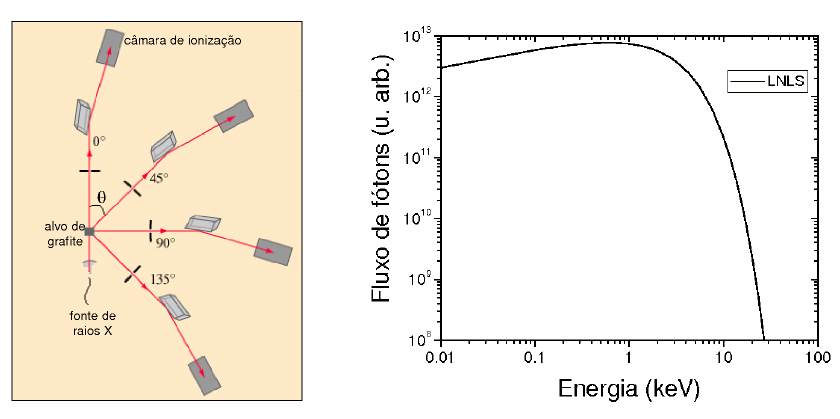
\includegraphics[scale=0.7]{classica-img/energia.png}
\caption{Período em função da energia para o pêndulo na aproximação de pequenas oscilações em torno de $\theta = 0$.}
\end{figure}


\item Um disco uniforme, de seção reta circular de raio $R$, massa $M$ e momento de inércia $I$ (com relação ao eixo perpendicular ao plano do disco e que passa pelo seu centro), encontra-se preso a uma mola de constante $k$, massa desprezível e um certo comprimento de repouso, como é mostrado na figura abaixo. O disco rola sobre a superfície sem deslizar e seu movimento está confinado ao plano da figura.
\begin{figure}[H]
\centering
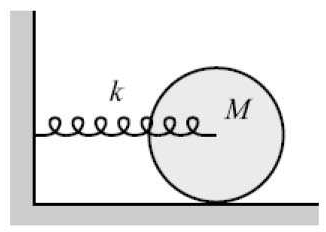
\includegraphics[scale=0.7]{classica-img/mola.png}
\end{figure}

a) Escreva a equação para a energia mecânica do sistema em função da velocidade do centro de massa e da distensão da mola.

\resposta Note que há um vínculo: $\theta = \frac{x}{R} \ \Rightarrow \ \dot{\theta} = \frac{\dot{x}}{R}$.
$$
T = \frac{I \dot{\theta}^{2}}{2} + \frac{M \dot{x}^{2}}{2}; \ \ V = \frac{k x^{2}}{2}
$$
Como a densidade é uniforme: $\sigma = \frac{M}{\pi R^{2}}$.

Apenas para fazer uma observação adicional, calcularei o momento de inércia do cilindro, cujo raio é $R$ e cuja distribuição de massa é uniforme. A distância do eixo do cilindro a um ponto arbitrário será batizada de $r$. O eixo de rotação desse cilindro se encontra no centro deste, de forma que temos a seguinte integral:
$$
\begin{array}{ccl}
  I = \int \int r^{2} dm  & = & \int \int r^{2} \sigma(r) d^{2} r = \int_{0}^{R} \int_{0}^{2\pi} r^{2} d m \\
   & = & \int_{0}^{R} \int_{0}^{2\pi} \frac{M r^{3}}{\pi R^{2}} dr d\theta = \frac{2M}{R^{2}} \int_{0}^{R} r^{3} dr = \frac{2 M R^{4}}{4R^{2}} = \frac{MR^{2}}{2}
\end{array}
$$
Vê-se que:
$$
 E = T + V = \frac{kx^{2}}{2} + \frac{I \dot{\theta}^{2}}{2} + \frac{M \dot{x}^{2}}{2}
 $$
Apenas vou utilizar o vínculo para expressar tudo em termos da coordenada $x$:
$$
 E = \frac{kx^{2}}{2} + \frac{\dot{x}^{2}}{2} \left( M + \frac{I}{R^{2}}  \right) = \frac{kx^{2}}{2} + \frac{3M \dot{x}^{2}}{4}
$$



b) Obtenha a equação de movimento para o centro de massa do disco.

\resposta

Sabemos que:
$$
 L = T - V =  \frac{\dot{x}^{2}}{2} \left( M + \frac{I}{R^{2}}  \right) - \frac{kx^{2}}{2} = \frac{3M \dot{x}^{2}}{4} - \frac{kx^{2}}{2}
$$
A equação de Euler-Lagrange é dada por:
$$
\frac{d}{dt} \left( \frac{\partial L}{\partial \dot{x}}  \right) - \frac{\partial L}{\partial x} = 0
$$
$$
\frac{\partial L}{\partial x} = -kx
$$
$$
\frac{\partial L}{\partial \dot{x}} = \left( M + \frac{I}{R^{2}}  \right) \dot{x} = \frac{3M}{2} \dot{x} \ \Rightarrow \ \frac{d}{dt} \frac{\partial L}{\partial \dot{x}} = \left( M + \frac{I}{R^{2}}  \right) \ddot{x} = \frac{3M}{2} \ddot{x}
$$
Logo, a equação de movimento do centro de massa é:
$$
\left( M + \frac{I}{R^{2}}  \right) \ddot{x} + kx = 0 \ \Rightarrow \ \ddot{x} + \left(\frac{k}{M + I/R^{2}}  \right) x = 0 \ \Rightarrow \ \ddot{x} + \frac{2k}{3M} x = 0
$$


c) Determine a frequência angular de oscilação do centro de massa do disco.


\resposta Através da equação de movimento, vemos que a frequência angular é:
$$
\omega = \sqrt{\frac{k}{M + I/R^{2}}} = \sqrt{\frac{2k}{3M}}
$$


\item Uma partícula de massa $m$ move-se em um potencial $V(r) = -C/(3r^{3})$, sendo $C$ uma constante positiva. Considere que a partícula possua momento angular $L$ diferente de zero.

a) Escreva a equação para a energia mecânica da partícula em termos da distância $r$ à origem, da sua derivada temporal $\dot{r}$, do momento angular $L$, da massa $m$ e da constante $C$.

\resposta A energia cinética de um potencial tipo central é:
$$
T = \frac{m \dot{r}^{2}}{2} + \frac{m r^{2} \dot{\theta}^{2}}{2} = \frac{m \dot{r}^{2}}{2} + \frac{L^{2}}{2 m r^{2}}
$$
Sendo $L = mr^{2} \dot{\theta}$. Para um potencial central vale a expressão:
$$
E = T + V = \frac{m \dot{r}^{2}}{2} + \frac{m r^{2} \dot{\theta}^{2}}{2} - \frac{C}{3r^{3}} = \frac{m \dot{r}^{2}}{2} + \frac{L^{2}}{2 m r^{2}} - \frac{C}{3r^{3}}
$$


b) Considerando os termos que só dependem de $r$ na energia mecânica como um potencial efetivo $V_{ef}(r)$, esboce o gráfico de $V_{ef}(r)$.

\resposta Utilizando a sugestão do enunciado:
$$
V_{ef}(r) = \frac{L^{2}}{2mr^{2}} - \frac{C}{3r^{3}}
$$
O gráfica é
\begin{figure}[H]
  \centering
  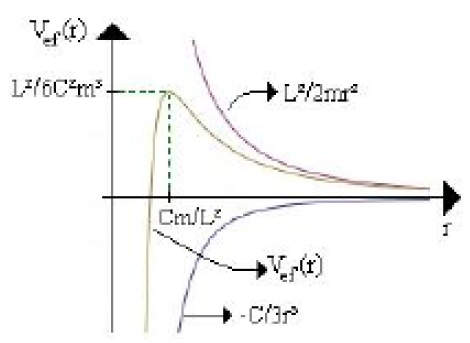
\includegraphics[scale=0.7]{classica-img/potencial}
  \caption{Gráfico do potencial efetivo, $V_{ef}(r)$, juntamente com os gráficos de $\frac{L^{2}}{2mr^{2}}$ e $\frac{-C}{3r^{3}}$.}
\end{figure}

c) Existem órbitas circulares para essa partícula? Em caso afirmativo, determine o raio de cada uma dessas possíveis órbitas e discuta a estabilidade das mesmas.

\resposta De fato, existem órbitas circulares para a partícula, pois:
$$
\left. \frac{\partial V_{ef}(r)}{\partial r} \right|_{r_{0}} = 0 \ \Rightarrow \ \left. \frac{\partial}{\partial r} \left( \frac{L^{2}}{2mr^{2}} - \frac{C}{3r^{3}} \right) \right|_{r_{0}} = \left. \left( \frac{C}{r^{4}} - \frac{L^{2}}{mr^{3}} \right) \right|_{r_{0}}
$$
$$
\Rightarrow \ \frac{C}{r_{0}^{4}} = \frac{L^{2}}{mr_{0}^{3}} \ \Rightarrow \ \left\{ \begin{array}{ccc}
                                           r_{0} & = & 0 \\
                                           r_{0} & = & \frac{Cm}{L^{2}}
                                         \end{array} \right.
$$
A primeira solução não é válida (as funções não são definidas em zero). Portanto, é possível a ocorrência de órbita para:
$$
r_{0} = \frac{Cm}{L^{2}}
$$
Sobre a estabilidade da órbita, devemos analisar a derivada segunda:
$$
\left. \frac{\partial^{2} V_{ef}(r)}{\partial r^{2}} \right|_{r_{0}} = \left. \left( \frac{3L^{2}}{mr^{4}} - \frac{4C}{r^{5}} \right) \right|_{r_{0}} = \frac{3L^{10}}{C^{4} m^{5}} - \frac{4L^{10}}{C^{4}m^{5}} = - \frac{L^{10}}{C^{4}m^{5}} < 0 \therefore \mbox{ a órbita é instável}
$$
Essa informação poderia ser retirada do gráfico, se notarmos que pequenas perturbações do sistema não levam-no de volta ao ponto de equilíbrio.


d) Calcule a energia mecânica mínima, $E_{min}$, acima da qual a partícula vinda do infinito é capturada pelo potencial, ou seja, não retorna mais para o infinito.

\resposta Se $E > V_{ef}(r_{0})$ ocorre a 'captura' da partícula:
$$
V_{ef} = \frac{L^{2}}{2mr_{0}^{2}} - \frac{C}{3r_{0}^{3}} = \frac{L^{6}}{2C^{2}m^{3}} - \frac{L^{6}}{2C^{2}m^{3}} = \frac{L^{6}}{6C^{2}m^{3}}
$$
Essa é a energia mecânica mínima necessária para que uma partícula vinda do infinito seja 'capturada'.









\item Considere um corpo de massa $m$ preso a uma mola de constante elástica $k$ e sujeito a uma força externa $F(t) = F_{0} \mathrm{cos} (\omega t)$. Suponha que o movimento da massa seja unidimensional e despreze as forças de atrito.


a) Escreva a equação de movimento.

\resposta

b) Obtenha a solução geral da equação homogênea, $x_{h}(t)$, e uma solução particular da equação não-homogênea, $x_{nh}(t)$.

\resposta

c) Escreva a solução total $x(t)$ e imponha as condições iniciais $x(0) = x_{0}$ e $\dot{x}(0) = 0$.

\resposta
  
d) Obtenha $x(t)$ no limite $\omega \rightarrow \omega_{0}$, onde $\omega_{0} = \sqrt{k/m}$.

\resposta


\item Considere uma partícula de massa $m$ mmovendo-se sob a ação do potencial central $V(r) = k(r/r_{0})^{4}$ onde $k$ e $r_{0}$ são constantes positivas. Em coordenadas polares o movimento radial é dado pela equação $m\ddot{r} = - d V_{ef}/dr$ onde $V_{ef} = V(r) + L^{2}/(2mr^{2})$ e $L = mr^{2} \dot{\theta}$ é o momento angular perpendicular ao plano do movimento.


a) Faça um esboço do potencial efetivo.

\resposta

b) Encontre a distância $a$ da partícula ao centro de forças para que seu movimento seja uma órbita circular com momento angular $L = 2 r_{0} \sqrt{mk}$. Calcule o valor das energias cinética, potencial e total nesta órbita.

\resposta

c) Calcule o período de rotação deste movimento circular.

\resposta

d) Se a partícula em órbita circular sofrer uma pequena perturbação que não altere o valor de $L$ ela começará a oscilar em torno da órbita original. Calcule o período de pequenas oscilações radiais deste movimento.

\resposta




\end{enumerate}








%
%
\chapter{Eletromagnetísmo}


\begin{enumerate}[start=1,label={\bfseries Q\arabic*.}]



\item Um solenoide muito longo, de seção reta circular de raio $R$, com $n$ voltas por unidade de comprimento, tem uma corrente elétrica dada por $I(t) = I_{0} \sin \omega t$. Seu eixo encontra-se ao longo do eixo $z$ de um sistema de coordenadas. Assuma o limite quase-estático ($\omega R << c$) e que o campo magnético \textbf{B} fora do solenoide é nulo.

a) Calcule o vetor campo magnético \textbf{B} dentro do solenoide.

\resposta

Por simetria, $\mathbf{B} = B\hat{z}$. A lei de Ampère é válida no limite quase-estático. Aplicando-a a um circuito retangular com dois lados paralelos de comprimento $L$ na direção $z$, sendo um dentro do solenoide e outro fora, e os dois outros lados na direção radial,

$$
\oint \mathbf{B} \cdot \mathrm{d} \mathbf{l}=B_{z} L=\mu_{0} I(S)=\mu_{0} n L I(t) \Rightarrow \mathbf{B}=\mu_{0} n I_{0} \sin (\omega t) \hat{\mathbf{z}} \quad(r<R)
$$

onde I(S) é a corrente total que atravessa o circuito e usamos que a contribuição dos lados radiais do circuito para a circulação de B é nula (porque $\mathbf{B}  \bot  dl$) e o campo magnético é nulo fora do solenoide.


b) Calcule o vetor campo elétrico \textbf{E} dentro do solenoide.

\resposta

Usando a lei de indução de Faraday

$$
\oint \mathbf{E} \cdot \mathrm{d} \mathbf{l}=-\frac{\mathrm{d}}{\mathrm{d} t} \iint \mathbf{B} \cdot \hat{\mathbf{n}} \mathrm{d} \mathbf{S}
$$

aplicada a um circuito circular de raio $r < R$, com eixo ao longo de $z$ e concêntrico ao solenoide ($\hat{n} = \hat{z}$) e usando que, por simetria, o campo elétrico é azimutal $\mathbf{E} = E\hat{\theta}$

$$
E 2 \pi r=-\pi r^{2} \frac{\mathrm{d}}{\mathrm{d} t} B, \Rightarrow \mathrm{E}(\mathrm{r})=-\frac{1}{2} \mu_{0} n \omega I_{0} r \cos (\omega t) \hat{\theta} \quad(r<R)
$$



c) Calcule o vetor campo elétrico \textbf{E} fora do solenoide.

Procedendo de maneira análoga ao item anterior mas agora com $r > R$

$$
E 2 \pi r=-\pi R^{2} \frac{\mathrm{d}}{\mathrm{d} t} B, \Rightarrow \mathrm{E}(\mathrm{r})=-\frac{1}{2 r} \mu_{0} n \omega I_{0} R^{2} \cos (\omega t) \hat{\theta} \quad(r>R)
$$

\resposta

Procedendo de maneira análoga ao item anterior mas agora com $r > R$

$$
E 2 \pi r=-\pi R^{2} \frac{\mathrm{d}}{\mathrm{d} t} B, \Rightarrow \mathrm{E}(\mathrm{r})=-\frac{1}{2 r} \mu_{0} n \omega I_{0} R^{2} \cos (\omega t) \hat{\theta} \quad(r>R)
$$








\item Um circuito RC é composto de um resistor de resistência $R$ ligado em série a um capacitor de capacitância $C$. No instante $t = 0$, uma bateria de voltagem $V$ é conectada ao circuito. O capacitor, inicialmente descarregado, consiste em duas placas metálicas circulares de raio $a$ separadas por uma distância $d$ (d << a) e com vácuo entre elas. Despreze efeitos de borda no capacitor, ou seja, considere o campo elétrico uniforme entre as placas e nulo fora delas. Assuma o limite quase-estático.



a) Calcule a capacitância $C$ do capacitor.

\resposta

A densidade superficial de carga $\sigma$ na placa com carga total $Q$ é relacionada ao campo elétrico $E$ entre as placas por $\sigma = Q/ \pi a^{2}) = \epsilon_{0} E$. A diferença de potencial entre as placas $U$ é relacionada ao campo elétrico por $E = U / d$. Como, por definição, $Q = CU$, segue que

$$
C=\frac{\epsilon_{0} \pi a^{2}}{d}.
$$



b) Calcule a corrente elétrica no circuito como função do tempo para $t > 0$.

\resposta

Pela lei de Kirchhoff

$$
V=R I+\frac{Q}{C}=R \frac{\mathrm{d} \mathrm{Q}}{\mathrm{d} t}+\frac{Q}{C}
$$

A solução dessa equação diferencial que satisfaz a condição inicial $Q(0) = 0$ é

$$
Q=V C\left(1-e^{-t / \tau}\right), \operatorname{com} \tau=R C
$$

Segue que,

$$
I=\frac{\mathrm{d}}{\mathrm{d} t} Q=\frac{V}{R} e^{-t / \tau}.
$$


c) Calcule o vetor campo magnético \textbf{B} nas bordas laterais da regi˜ao entre as placas do capacitor como função do tempo para $t > 0$.

\resposta

Como a carga (e o campo elétrico) no capacitor muda(m), campo magnético é gerado. Aplicaremos a lei de Ampère-Maxwell

$$
\oint \mathbf{B} \cdot \mathrm{d} \mathbf{l}=\mu_{0} \int \mathbf{J} \cdot \hat{\mathbf{n}} \mathrm{d} S+\mu_{0} \epsilon_{0} \frac{\mathrm{d}}{\mathrm{d} t} \int \mathbf{E} \cdot \hat{\mathbf{n}} \mathrm{d} S
$$

a um circuito circular de raio $a$ paralelo às placas do capacitor, a meio caminho entre elas e com centro no seu eixo. Nesse caso, $\mathbf{J} = 0$ e $\hat{\mathbf{n}} || \mathbf{E} = \frac{\sigma}{\epsilon_{0}} \hat{z}$. Além disso, $\mathbf{B} = B\hat{\theta}$ (por simetria). Segue que

\begin{eqnarray*}
B 2 \pi a &=& \mu_{0} \epsilon_{0} \frac{\mathrm{d}}{\mathrm{d} t} \int E \mathrm{d} S=\mu_{0} \epsilon_{0} \frac{\mathrm{d}}{\mathrm{d} t} \int \frac{Q(t)}{\epsilon_{0} \pi a^{2}} \mathrm{d} S=\mu_{0} \frac{\mathrm{d}}{\mathrm{d} t} Q(t)=\mu_{0} I(t) \\
&\Rightarrow & \quad \mathrm{B}=\frac{\mu_{0} I(t)}{2 \pi a} \hat{\theta}
\end{eqnarray*}



d) Calcule o vetor de Poynting e a taxa temporal de energia eletromagnética entrando na regi˜ao entre as placas do capacitor enquanto ele é carregado.

\resposta

O vetor de Poynting na borda do capacitor é

$$
\mathrm{S}=\frac{1}{\mu_{0}} \mathbf{E} \times \mathbf{B}=\frac{Q(t)}{\epsilon_{0} \pi a^{2}} \hat{\mathbf{z}} \times \frac{I(t)}{2 \pi a} \hat{\boldsymbol{\theta}}, \Rightarrow \mathbf{S}=-\frac{Q I}{\epsilon_{0} 2 \pi^{2} a^{3}} \hat{\mathbf{r}}
$$

A taxa temporal de energia eletromagnética que flui para dentro do capacitor é a integral do módulo do vetor de Poynting na sua área lateral

$$
P=S 2 \pi a d=\frac{Q I d}{\epsilon_{0} \pi a^{2}}=I E d=I U
$$
onde, como antes, U é a diferença de potencial entre as placas.







\item Um disco de raio $a$ feito de um material isolante gira em torno do seu eixo de simetria com velocidade angular $\omega$ constante. Uma espira de cobre, na forma de um setor circular de ângulo $\pi/4$ e mesmo raio $a$, está presa à superfície do disco como mostra a figura abaixo. A resistência elétrica da espira é $R$. Um campo magnético externo de módulo $B$, perpendicular ao disco e entrando no plano da figura, está presente na região do espaço delimitada pelos ângulos fixos $\theta = \pi/4$ e $\theta = 3 \pi/4$.

\begin{figure}[H]
\centering
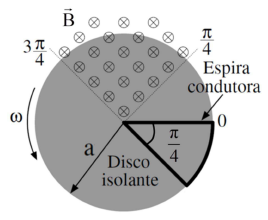
\includegraphics[scale=0.8]{eletromag-img/espira}
\end{figure}



a) Calcule o módulo da corrente elétrica induzida na espira quando esta entra ou sai da região de campo magnético.

\resposta

b) Convencionando como positiva a corrente que circula na espira no sentido horário, faça o gráfico da corrente induzida como função do tempo para o intervalo de tempo de uma de uma revolução do disco. Considere como instante inicial aquele ilustrado na figura.

\resposta

c) Calcule a energia total dissipada na espira em um ciclo.

\resposta

d) Calcule o torque da força magnética sobre a espira, com relação ao centro do disco, quando ela entra na região de campo magnético. Além do módulo, determine a direção e o sentido do \textbf{vetor} torque.

\resposta




\item Uma esfera condutora maciça de raio $R$ está carregada e imersa simetricamente entre dois dielétricos de permissividades elétricas $\textepsilon_{1}$ e $\textepsilon_{2}$, conforme ilustrado na figura abaixo. Resolvendo-se a equação de Laplace, pode-se mostrar que o potencial eletrostático fora da esfera ($r > R$) é dado por $V(\vec{r}) = A/r$, sendo $A$ uma constante e $r = |\vec{r}|$. Expresse as suas respostas em termos de $A$, $R$, $\textepsilon_{1}$, $\textepsilon_{2}$, e da posição $\vec{r}$.

\begin{figure}[H]
\centering
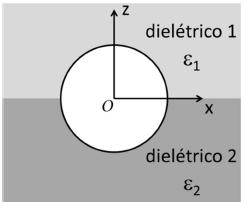
\includegraphics[scale=1]{eletromag-img/dieletrico}
\end{figure}


a) Calcule o potencial eletrostático $V(\vec{r})$ e o campo elétrico $\vec{E}(\vec{r})$ no interior da esfera ($r < R$).

\resposta

b) Calcule o campo elétrico $\vec{E}(\vec{r})$ e o deslocamento elétrico $\vec{D}(\vec{r})$ fora da esfera ($r > R$), em cada dielétrico (dielétrico 1 e dielétrico 2).

\resposta

c) Quais são as densidades superficiais de carga livre na superfície da esfera condutora adjacente a cada um dos dielétricos?

\resposta

d) Há carga de polarização na interface entre os dois dielétricos? Se sim, quanto vale a densidade superficial dessa carga? Se não, justifique.

\resposta




\item Um capacitor de placas paralelas condutoras tem suas duas placas perpendiculares à direção $z$. Uma das placas, localizada em $z = 0$, tem um potencial elétrico $V = 0$, enquanto a outra placa, localizada em $z = d$, tem um potencial elétrico $V = V_{0}$, onde $V_{0}$ é uma constante. No espaço entre as placas, preenchido por um dielétrico com permissividade elétrica $\epsilon$, a densidade de carga elétrico livre é dada por
$$
\rho_{F}(z) = \rho_{0} e^{-\alpha z},
$$
onde $\rho_{0}$ e $\alpha$ são constantes. Despreze os efeitos de borda.



a) Mostre que o potencial entre as placas é da forma
$$
V(z) = A + Bz - \frac{\rho_{0}}{\epsilon \alpha^{2}} e^{\alpha z},
$$
onde $A$ e $B$ são constantes.

\resposta O problema se resume a resolver a equação de Poisson
$$
\nabla^{2} V = - \frac{\rho}{\epsilon}
$$
No nosso caso a simetria do problema dita que $V (\vec{r}) = V (z)$. Portanto,
$$
\nabla^{2} V = \frac{d^{2} V}{dz^{2}} = - \frac{\rho}{\epsilon} e^{-\alpha z}.
$$
Integrando a Eq. (8) uma vez em z teremos
$$
\frac{dV}{dz} = B + \frac{\rho_{0}}{\epsilon \alpha} e^{-\alpha z}.
$$
Integrando agora a Eq. (9) uma vez em $z$ teremos finalmente
$$
V(z) = A + Bz + \frac{\rho_{0}}{\epsilon \alpha} e^{-\alpha z}
$$
onde $A$ e $B$ são constantes de integração.



b) Determine as constantes $A$ e $B$ a partir das condições de contorno.

\resposta Impondo as condições de contorno,
$$
V(z=0) = 0 \Rightarrow 0 = A - \frac{\rho_{0}}{\epsilon \alpha^{2}} \Rightarrow A = \frac{\rho_{0}}{\epsilon \alpha^{2}}.
$$
$$
V(z=d)=V_{0} \Rightarrow V_{0}=A+B d-\frac{\rho_{0}}{\epsilon \alpha^{2}} e^{-\alpha d} \Rightarrow B=\frac{1}{d}\left[V_{0}+\frac{\rho_{0}}{\epsilon \alpha^{2}}\left(e^{-\alpha d}-1\right)\right].
$$

c) Determine o \textbf{vetor} campo elétrico entre as placas.

\resposta Do item (b), o potencial é dado por

$$
V(z)=\frac{\rho_{0}}{\epsilon \alpha^{2}}+\frac{1}{d}\left[V_{0}+\frac{\rho_{0}}{\epsilon \alpha^{2}}\left(e^{-\alpha d}-1\right)\right] z-\frac{\rho_{0}}{\epsilon \alpha^{2}} e^{-\alpha z}
$$
Temos que
$$
\mathrm{E}=-\nabla V=-\frac{\partial V}{\partial x} \hat{\mathrm{x}}-\frac{\partial V}{\partial y} \hat{\mathrm{y}}-\frac{\partial V}{\partial z} \hat{\mathrm{z}}=-\frac{d V}{d z} \hat{\mathrm{z}}
$$
Portanto
$$
\begin{aligned}
\mathbf{E} &=-\left\{\frac{1}{d}\left[V_{0}-\frac{\rho_{0}}{\epsilon \alpha^{2}}\left(1-e^{-\alpha d}\right)\right]+\frac{\rho_{0}}{\epsilon \alpha^{2}} \alpha e^{-\alpha z}\right\} \hat{\mathbf{z}} \\
&=\frac{1}{d}\left[\frac{\rho_{0}}{\epsilon \alpha^{2}}\left(1-e^{-\alpha d}-\alpha d e^{-\alpha z}\right)-V_{0}\right] \hat{\mathbf{z}}
\end{aligned}
$$








\item a) Um segmento retilíneo de fio, de comprimento $L$, transporta uma corrente $i$. Calcule o módulo do campo magnético $B$, produzido pelo segmento no ponto $P$, localizado a uma distância $R$ do segmento e equidistante de suas extremidades, como mostra a Figura (a).
\begin{figure}[H]
\centering
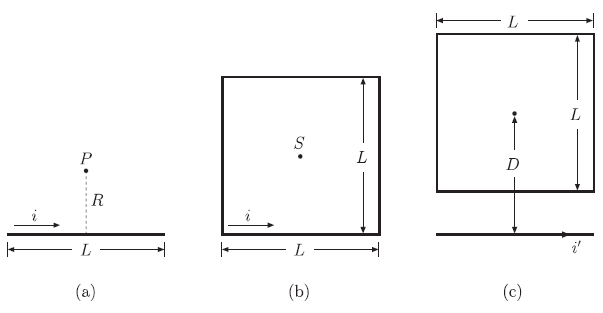
\includegraphics[scale=1]{eletromag-img/aros.png}
\end{figure}

\resposta A lei de Biot-Savart é

$$
\mathbf{B}(\mathbf{r})=\frac{\mu_{0} i}{4 \pi} \int_{C} \frac{d \mathbf{l}^{\prime} \times\left(\mathbf{r}-\mathbf{r}^{\prime}\right)}{\left|\mathbf{r}-\mathbf{r}^{\prime}\right|^{3}}
$$
Tomando um sistema de referência tal que $d \mathrm{l}^{\prime}=d x^{\prime} \hat{\mathrm{x}}, \mathrm{r}^{\prime}=x^{\prime} \hat{\mathrm{x}}$ e $\mathrm{r}=R \hat{\mathrm{y}}$
$$
\mathbf{B}(P)=\frac{\mu_{0} i}{4 \pi} \int_{-L / 2}^{L / 2} \frac{R d x^{\prime} \hat{\mathbf{z}}}{\left(R^{2}+x^{\prime 2}\right)^{3 / 2}}=\frac{\mu_{0} i R}{2 \pi} \int_{0}^{L / 2} \frac{d x^{\prime}}{\left(R^{2}+x^{2}\right)^{3 / 2}} \hat{\mathbf{z}}
$$
Usando a integral fornecida no formulário
$$
\mathbf{B}(P)=\frac{\mu_{0} i}{2 \pi R} \frac{L}{\sqrt{4 R^{2}+L^{2}}} \hat{\mathbf{z}}
$$
Portanto,
$$
B(P)=\frac{\mu_{0} i}{2 \pi R} \frac{L}{\sqrt{4 R^{2}+L^{2}}}
$$



b) Use o resultado do item (a) e obtenha $B$ quando $R << L$. Compare o resultado com o módulo do campo magnético gerado por um fio muito longo.

\resposta A Eq. (10) no limite $R << L$ torna-se
$$
B = \frac{\mu_{0} i}{2 \pi R}.
$$
Este é o módulo do campo magnético gerado por um fio infinito, como obtido facilmente pela aplicação direta da lei de Ampère.


c) Considere agora uma espira quadrada de fio, de lado $L$, transportando uma corrente $i$, como na Figura (b). Calcule o módulo do campo magnético $B$ no ponto $S$, localizado no centro da espira.

\resposta A espira quadrada é formada pela junção de 4 segmentos de fio de comprimento $L$. Como as contribuições de cada segmento são vetorialmente idênticas, o campo no centro da espira será simplesmente a soma das contribuições individuais de cada segmento. O módulo resultante é, portanto,
$$
 B = \left.4 \frac{\mu_{0} i}{2 \pi R} \frac{L}{\sqrt{4 R^{2}+L^{2}}}\right|_{R=L / 2}=\frac{2 \sqrt{2} \mu_{0} i}{\pi L}
$$


d) Uma espira quadrada de fio, de lado $L$ e sem nenhuma corrente, é colocada próxima a um fio infinitamente longo que transporta uma corrente $i'$. A distância do fio longo ao centro da espira é $D$, como mostrado na Figura (c). Determine a intensidade do fluxo magnético gerado pelo fio através da espira.

\resposta O campo magnético gerado por um fio longo infinito, transportando uma corrente $i'$, em uma distância $r'$ do fio, é dado por
$$
\mathbf{B}=\frac{\mu_{0} i^{\prime}}{2 \pi r^{\prime}} \hat{z}
$$
O fluxo de campo magnético $\Phi_{B}$ através da superfície da espira é dado por
$$
\Phi_{B}=\int_{S} \mathbf{B} \cdot \hat{n} d a
$$
onde $d a=d x d y$ e $\hat{n}=\hat{\mathbf{z}},$ logo
$$
\mathbf{B} \cdot \hat{n}=\frac{\mu_{0} i^{\prime}}{2 \pi r^{\prime}}=\frac{\mu_{0} i^{\prime}}{2 \pi y}
$$
Portanto,
$$
\Phi_{B}=\int_{S} \frac{\mu_{0} i^{\prime}}{2 \pi y} d x d y=\frac{\mu_{0} i^{\prime}}{2 \pi} \int_{-L / 2}^{L / 2} d x \int_{D-L / 2}^{D+L / 2} \frac{d y}{y}=\frac{\mu_{0} i^{\prime}}{2 \pi} L \ln \left(\frac{2 D+L}{2 D-L}\right)
$$





\item Um espectrômetro de massa simples pode ser construído como esquematizado na figura. Um feixe de íons positivos de massa $m$ e carga $q$  (linha pontilhada) sai de uma fonte $S$, é acelerado pela diferença de potencial elétrico $V$ e penetra por uma fenda de entrada numa câmara onde há um campo magnético uniforme $B$ saindo perpendicularmente do plano do papel. Após percorrer uma trajetória semicircular de raio $r$, o feixe sai pela fenda de saída e é detectado por um deterctor $D$ se a massa for compatível com a trajetória. Dessa forma, é possível selecionar íons pelo valor de sua massa, ajustando o valor de $B$. As fendas de entrada e de saída da câmara são iguais. Todo o sistema está em vácuo. Despreze a interação gravitacional do feixe.

\begin{figure}[H]
\centering
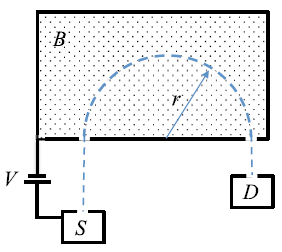
\includegraphics[scale=1]{eletromag-img/espec.png}
\end{figure}




a) Determine o módulo da velocidade dos íons ao passarem pela fenda de saída em termo de $V$, $m$ e $q$.

\resposta

b) Determine $m$ em função de $V$, $B$, $r$ e $q$.

\resposta

c)A resolução das medidas de massa do aparelho é limitada pelo tamanho da fenda de saída,que determina o erro do raio $r$. Considere uma situação em que $r = 10 cm$, $V = 4,0 \times 10^{3} \mbox{V}$, $B = 1,00 \mbox{T}$ e que cada íon tem um elétron a menos que o átomo neutro correspondente. Se as fendas têm tamanho $100 \ \mu m$, qual é a resolução das medidas de massa?

\resposta

d) É possível usar esse aparelho para distinguir os isótopos de carbono $^{12}\mbox{C}$ de $^{14}\mbox{C}$? Justifique.

\resposta




\item Considere a propagação de ondas eletromagnéticas num meio linear, homogêneo e istrópico com condutividade elétrica $\sigma$, permissividade elétrica $\epsilon$ e permeabilidade magnética $\mu$, na ausência de fontes de cargas elétricas livres ($\rho_{F} = 0$).


a) Escreva as equações de Maxwell para os campos elétrico $\mathbf{E}$ e magnético $\mathbf{B}$ no meio, em termos de $\sigma$, $\epsilon$ e $\mu$.

\resposta

b) Encontre a equação diferencial que envolve apenas o campo elétrico $\mathbf{E}$.

\resposta

c) Considere uma solução do tipo onda plana $\mathbf{E}(x,t) = \mathbf{E}_{0} e^{i(kx - \omega t)}$ e obtenha a relação entre $k$ e $\omega$ em termos de $\sigma$, $\epsilon$ e $\mu$.

\resposta

d) Com relação ao resultado do item (c), interprete fisicamente a diferença entre os casos $\sigma \neq 0$ e $\sigma = 0$.

\resposta




\item Considere o circuito representado na figura. Inicialmente, o capacitor está descarregado. No instante $t=0$ a chave $S_{1}$ é fechada.

\begin{figure}[H]
\centering
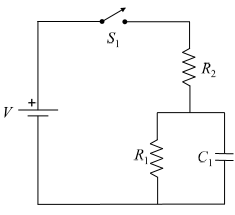
\includegraphics[scale=1]{eletromag-img/quadrada.png}
\end{figure}


a) Quais são os valores da corrente que passa pelo resistor de resistência $R_{1}$ em $t = 0$ e após um longo tempo?

\resposta

b) Qual é a carga no capacitor de capacitância $C_{l}$ após um longo tempo?

\resposta

c) Faça três gráficos esquemáticos das diferenças de potencial como funções do tempo entre as extremidades dos resistores de resistências $R_{1}$ e $R_{2}$ e do capacitor de capacitância $C_{1}$ a partir de $t = 0$, indicando claramente os valores máximos e mínimos.

\resposta

d) Depois de permanecer ligada por um longo tempo, a chave $S_{1}$ é desligada em $t = t_{d}$. Quanto tempo então decorre para que a carga do capacitor caia para uma fração $l/e$ do seu valor em $t = t_{d}$? ($e \approx 2.718$ é a base dos logaritmos naturais)

\resposta





\item Um guia de ondas muito usado em laboratórios é o cabo coaxial. Ele consiste de um fio condutor interno rodeado por um isolante (branco) dentro de uma malha condutora, protegida por um encapamento isolante (preto), como mostrado na foto da esquerda. Ele pode ser modelado como um fio metálico interno de raio a dentro de um dielétrico com permissividade elétrica 6 e permeabilidade magnética p e uma casca metálica cilíndrica de raio interno b, como indicado na figura da direita. A corrente percorre o fio interno numa direção e a casca cilíndrica na direcão contrária.

\begin{figure}[H]
\centering
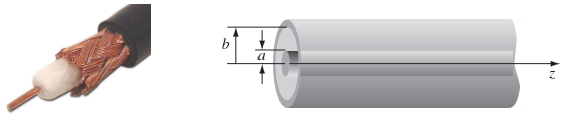
\includegraphics[scale=1]{eletromag-img/coaxial.png}
\end{figure}


\item(a) Use a simetria do problema e a lei de Gauss para obter a capacitância por unidade de comprimento do cabo em termos de e, V, a e b.

\resposta

\item(b) Use a simetria do problema e a lei de Ampàre para obter a auto-indutância por unidade de comprimento do cabo em termos de e, V, a e b. Dica: calcule a energia armazenada no campo magnético em um comprimento finito do cabo e iguale o resultado a LI 2/2, onde L é a auto-indutância e I é a corrente pelo cabo.

\resposta





\item Um anel fino de raio $R$ e carga total $Q > 0$ uniformemente distribuída ao longo de sua circunferência está fixo no plano $xy$ de um sistema de coordenadas e tem seu centro na origem $O$. Seja $P$ um ponto com coordenadas $(0,0,z)$ (ver figura abaixo).
\begin{figure}[H]
\centering
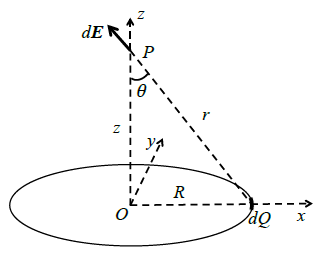
\includegraphics[scale=1]{eletromag-img/anel.png}
\end{figure}

a) Somando as contribuições de todos os elementos de carga do anel, encontre módulo, direção e sentido do campo elétrico $\vec{E}(z)$ no ponto $P$.

\resposta O elemento de carga $d Q$ do anel produzirá um campo $d \vec{E}$ no ponto $P$, como mostrado na figura. O mádulo deste elemento de campo elétrico é
$$
d E = \frac{d Q}{4 \pi \epsilon_{0} r^{2}}.
$$
\begin{figure}[H]
  \centering
  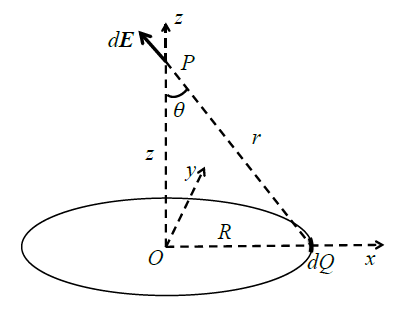
\includegraphics[scale=0.7]{eletromag-img/anel3.png}
  %\caption{}\label{}
\end{figure}
A componente deste elemento de campo elétrico perpendicular ao eixo $z$ é cancelada pela componente perpendicular ao eixo $z$ produzida pelo elemento de carga situado na posição diametralmente oposta do anel. Ao somar os elementos de campo elétrico devido a todos os elementos de carga do anel, apenas sobrevivem as componentes na direção do eixo $z$
$$
d E_{z}=\frac{d Q}{4 \pi \epsilon_{0} \tau^{2}} \cos \theta=\frac{d Q}{4 \pi \epsilon_{0} r^{2}} \frac{z}{r}
$$
Somando todas as contribuições dos elementos de carga do anel, obtemos
$$
\vec{E}=\hat{z} \frac{Q z}{4 \pi \epsilon_{0} r^{3}}=\hat{z} \frac{Q z}{4 \pi \epsilon_{0}\left(R^{2}+z^{2}\right)^{3 / 2}}
$$


b) Proceda analogamente ao item (a) e calcule o potencial elétrico $V (z)$ no ponto $P$.

\resposta O potencial elétrico devido ao elemento de carga $d Q$ no ponto $P é$
$$
d V(z)=\frac{d Q}{4 \pi \epsilon_{0} r}
$$
O potencial devido a todas as contribuições dos elementos de carga do anel é obtido somando todas as contribuições, donde se obtém
$$
V(z)=\frac{Q}{4 \pi \epsilon_{0} r}=\frac{Q}{4 \pi \epsilon_{0} \sqrt{R^{2}+z^{2}}}
$$


c) Uma partícula pontual de carga $- q < 0$ e massa $m$ parte do repouso de um ponto com coordenadas $(0,0,z_{0})$, muito distante da origem (ou seja, $z_{0} >> R$) e viaja ao longo do eixo $z$. Qual é a sua velocidade quando ela passa pelo centro do anel? Considere desprezíveis os efeitos da radiação eletromagnética emitida pela partícula no seu trajeto em direção ao centro do anel.

\resposta A energia cinética inicial da partícula é nula, porque ela parte do repouso. A energia potencial elétrica inicial da partícula é nula também, porque $-q V\left(z_{0}\right) \approx 0$ se $z_{0} \gg R$. A conservação da energia mecânica (cinética mais potencial elétrica) nos dá a velocidade $v$ no centro do anel via
$$
0+0=\frac{m v^{2}}{2}+(-q) V(0)=\frac{m v^{2}}{2}-q \frac{Q}{4 \pi \epsilon_{0} R}
$$
donde
$$
v=\sqrt{\frac{q Q}{2 \pi \epsilon_{0} m R}}
$$





\item Um aro quadrado rígido de arame com lado $L$ tem resistência elétrica total $R$. O aro está no plano $xy$ de um sistema de coordenadas e move-se com velocidade $\vec{v}$ para fora da regi˜ao onde há um campo magnético uniforme $\vec{B}$ (area sombreada na figura abaixo) apontando para fora da página (sentido de $z$ positivo). Considere o instante em que o vértice da esquerda do aro está a uma distância $s$ dentro da area sombreada ($0 < s < \sqrt{2}L/2$).

\begin{figure}[H]
\centering
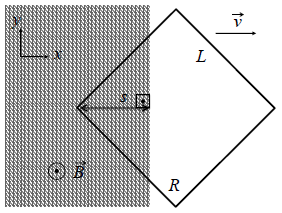
\includegraphics[scale=1]{eletromag-img/aro.png}
\end{figure}


a) Calcule o fluxo do campo magnético através do aro como função de $s$.

\resposta Como o aro $\hat{\epsilon}$ quadrado, a área da região interna ao aro e contida no retângulo sombreado
é um triângulo isósceles de altura $s$ e ângulos internos $45^{\circ}, 90^{\circ}$ e $45^{\circ} .$ Portanto, o tamanho da base do triângulo é 2 s e sua área é
$$
A=\frac{1}{2} s(2 s)=s^{2}
$$
O fluxo do campo magnético através do aro é
$$
\Phi=\int \vec{B} \cdot d \vec{S}=B A=B s^{2}
$$
onde usamos o fato de que o campo magnético $B$ constante na região sombreada e normal ao plano da figura.
\begin{figure}[H]
  \centering
  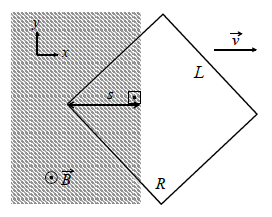
\includegraphics[scale=0.7]{eletromag-img/aro3}
 % \caption{}\label{}
\end{figure}



b) Determine o valor e o sentido de circulação da corrente elétrica induzida no aro.

\resposta b) A força eletromotriz induzida pode ser calculada pela lei de Faraday:
$$
\varepsilon=-\frac{d \Phi}{\partial t}=-B 2 s \frac{d s}{d t}=-2 B s v
$$
e o valor da corrente elétrica é
$$
I=\frac{2 B s v}{R}
$$
A área sombreada diminui com o movimento do aro e, portanto, o fluxo do campo magnético também diminui. O sentido da força eletromotriz, pela lei de Lenz, é anti-horário para se contrapor à diminuição do fluxo de $\bar{B}$. Segue que a corrente fluirá também no sentido anti horário.

c) Calcule a força magnética total (módulo, direção e sentido) sobre o aro quando a corrente induzida circula nele. Que força adicional à força magnética deve ser aplicada no aro para que ele se mova com velocidade constante sob a ação exclusiva dessas duas forças?

\resposta A força magnética sobre um elemento do aro é
$$
d \vec{F}_{m}=I d \vec{l} \times \vec{B}
$$
Os elementos do aro dentro da região sombreada são: $d \vec{l}=-\frac{\sqrt{2}}{2}(\hat{x} d l+\hat{y} d l)$ (lado superior esquerdo) e $d \vec{l}=\frac{\sqrt{2}}{2}(\hat{x} d l-\hat{y} d l)$ (lado inferior esquerdo). A força magnética é, então,
$$
d \vec{F}_{m}=I\left[-\frac{\sqrt{2}}{2}(\hat{x} d l+\hat{y} d l) \times B \hat{z}+\frac{\sqrt{2}}{2}(\hat{x} d l-\hat{y} d l) \times B \hat{z}\right]
$$
ou
$$
d \vec{F}_{m}=-\sqrt{2} I B d l \hat{x}
$$
e integrando em $d l$ de 0 a $\sqrt{2} s$ (lembrando que as contribuições dos dois segmentos já foram somadas) obtemos
$$
\vec{F}_{m}=-2 I B s \hat{x}
$$
Substituindo a Eq. (5) na Eq. (6), obtemos
$$
\vec{F}_{m}=-\hat{x} \frac{4 B^{2} s^{2} v}{R}
$$
Para que o quadrado se mova com velocidade constante, temos que aplicar uma força de mesmo módulo que $\vec{F}_{m},$ mas de sentido oposto, isto é para a direita (sentido positivo de $x$ ).






\item Dois aros circulares finos encontram-se no plano $xy$ de um sistema de coordenadas, ambos com centro na origem. Um aro tem raio $b$ e uma densidade linear de carga elétrica $-\lambda < 0$ e o outro tem raio $2b$ e uma densidade linear de carga elétrica $2 \lambda > 0$.


a) Calcule o potencial eletrostático $V (z)$ no ponto $P = (0,0,z)$.

\resposta

b) Calcule o vetor campo elétrico $\vec{E}(z)$ no ponto $P = (0,0,z)$.

\resposta

c) Escreva a equação da segunda lei de Newton para uma partícula de carga $q > 0$ e massa $m$, restrita a se mover ao longo do eixo $z$ e sujeita ao campo elétrico do item (b). Além da força elétrica, nenhuma outra força atua sobre a partícula.

\resposta

d) Calcule a frequência de pequenas oscilações para a partícula do item (c) na vizinhança de $z = 0$. Dica: linearize a força em torno de $z = 0$.




\item Uma onda eletromagnética plana monocromática que se propaga no vácuo com polarização circular é descrita, em notação complexa, pelo campo elétrico $\tilde{\mathbf{E}}(\mathbf{r},t) = E_{0}e^{i(kz-\omega t)} \left(\hat{X} + i \hat{Y} \right)$, onde $\omega = ck$ é a frequência angular, $c$ é a velocidade da luz no vácuo, $k$ é o número de onda, $E_{0}$ é uma amplitude real e $i = \sqrt{-1}$.


a) Encontre o campo elétrico real (físico) $\mathbf{E}(\mathbf{r},t)$.

\resposta

b) Encontre o campo magnético real (físico) $\mathbf{B}(\mathbf{r},t)$ usando as equações de Maxwell. Se preferir, utilize $\nabla \rightarrow ik$.

\resposta

c) Calcule a densidade de momento linear da onda eletromagnética $g = \epsilon_{0} \mathbf{E} \times \mathbf{B}$.

\resposta

d) Calcule a densidade de momento angular da onda eletromagnética $\mathbf{l} = \mathbf{r} \times \mathbf{g}$. Dica: use coordenadas cilíndricas $r = \rho \hat{\rho} + z \hat{z}$.



\item Definindo-se o vetor de Hertz $\vec{Z}$ pelas expressões:
\begin{equation}
\vec{\nabla} \cdot \vec{Z} = -\phi; \quad \vec{A} = \mu_{0} \epsilon_{0} \frac{\partial \vec{Z}}{\partial t},
\end{equation}

onde $\phi$ e $\vec{A}$ são, respectivamente, os potenciais escalar e vetor.


a) Mostre que os potenciais satisfazem o calibre de Lorentz:

\begin{equation}
\vec{\nabla} \cdot \vec{A} + \mu_{0} \epsilon_{0} \frac{\partial \phi}{\partial t} = 0;
\end{equation}

\resposta

b) Demonstre que para um meio sem fontes ($\rho = 0$, $\vec{J} = 0$) e de $\mu = \mu_{0}$ o vetor $\vec{Z}$ satisfaz às seguintes expressões:

\begin{equation}
\nabla^{2} \vec{Z} - \frac{1}{c^{2}} \frac{\partial^{2} \vec{Z}}{\partial t^{2}} = - \frac{\vec{P}}{\epsilon_{0}}; \quad
\vec{B} = \frac{1}{c^{2}} \vec{\nabla} \times \frac{\partial \vec{Z}}{\partial t}; \quad \vec{E} = \vec{\nabla} \times \vec{\nabla} \times \vec{Z} - \frac{\vec{P}}{\epsilon_{0}},
\end{equation}
onde $\vec{P}$ é o vetor de polarização.

\resposta

\item Considere um disco vazado muito fino, com raio interno $r_{1}$ e raio externo $r_{2}$, deitado sobre o plano $xy$ e com o eixo centrado em $z = 0$ (conforme ilustrado na figura 1).

\begin{figure}[H]
\centering
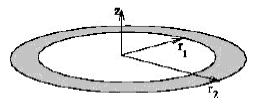
\includegraphics[scale=1]{eletromag-img/vasado.png}
\end{figure}

O anel tem densidade superficial de carga dada por:
\begin{equation}
\sigma (r) = \frac{\sigma_{0}}{r}
\end{equation}

onde $r  = \sqrt{x^{2} + y^{2}}$


a) Encontre o campo elétrico $\vec{E}(x = y = 0, z$) sobre o eixo $z$;

\resposta

b) Suponha agora que o anel comece a girar com velocidade angular $\omega_{0}$. Encontre a densidade de corrente $\vec{J}_{s} = \sigma \vec{v}$, onde $\vec{v}$ é a velocidade linear;

\resposta

c) Encontre o campo magnético $\vec{H}(x = y = 0;z)$ sobre o eixo $z$, gerado pela densidade de corrente $\vec{J}_{s}$.




\item Uma esfera isolante sólida de raio $a$ tem densidade de carga uniforme $\rho$ carga total $Q$. Uma esfera oca condutora não carregada, cujos raios interno e externo são $b$ e $c$, respectivamente, é concêntrica à esfera isolante, como mostra a figura abaixo.

\begin{figure}[H]
\centering
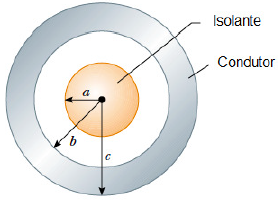
\includegraphics[scale=1]{eletromag-img/esfera.png}
\end{figure}


a) Determine a magnitude do campo elétrico nas regiões: $(i) \ r < a; \ (ii) \ a < r < b; \ (iii) \ b < r < c \ e \ (iv) \ r > c$.

\resposta Pela lei de Gauss, de maneira geral, sabemos que:
%
\begin{equation} \label{eq9}
  \oint \vec{E} \cdot d \vec{S} = \frac{q_{V}}{\epsilon_{o}}
\end{equation}
%
onde a integral é feita sobre a superfície $S$ de uma região $V$ e $q_{V}$ é a carga total contida em $V$. Tomaremos, nessa questão, regiões esféricas de raio $r$ centradas no centro da esfera isolante. Por simetria, o campo elétrico apontará sempre na direção radial, ou seja, $\vec{E} = E \hat{r}$.

i) Campo elétrico para $r < a$: Neste sub-item, escolhemos regiões esféricas de raio $r < a$, representadas pelas linhas pontilhadas na Fig. \ref{imagenspng}. Desta forma, a carga em $V$ é
%

\begin{equation}
  \begin{array}{ccc}
    q_{V} & = & \rho V \\
    q_{V} & = & \frac{4 \pi \rho}{3} r^{3} .
  \end{array}
\end{equation}
%

Aplicando a Eq. (\ref{eq9}) e usando que o campo elétrico é radial
\begin{equation}
  E 4 \pi r^{2} = \frac{4 \pi \rho}{3 \epsilon_{o}} r^{3} .
\end{equation}
%
Portanto, a magnitude do campo elétrico será dada por
%
\begin{equation}
  E = \frac{\rho}{3 \epsilon_{o}} r .
\end{equation}
%
ii) Campo elétrico para $a < r < b$: Neste caso, as regiões esféricas tem raio $r$ tal que $a < r < b$, como mostrado na Fig. \ref{figuraspng}. A carga total contida em $V$ é $q_{V} = Q$. Aplicando a Eq. (\ref{eq9}) e usando que o campo elétrico é radial
%
\begin{equation}
  E 4 \pi r^{2} = \frac{Q}{\epsilon_{o}} .
\end{equation}
%
Portanto, a magnitude do campo elétrico será
%
\begin{equation}
  E = \frac{Q}{4 \pi \epsilon_{o} r^{2}}
\end{equation}
%

iii) Campo elétrico para $b < r < c$: Nesta região, queremos o campo elétrico dentro de um condutor em equilíbrio eletrostático (veja a Fig. \ref{figuraspng}), que sempre se anula. Portanto,
%

$$
E = 0 .
$$
%

(iv) Campo elétrico para $r > c$: Agora, as regiões esféricas tem raio $r > c$, como mostrado na Fig. \ref{figuraspng}. A carga contida em $V$ é $q_{V} = Q$. Aplicando novamente a Eq. (\ref{eq9}) e usando que o campo elétrico é radial

%
\begin{equation}
  E 4 \pi r^{2} = \frac{Q}{\epsilon} .
\end{equation}
%
Portanto, a magnitude do campo elétrico será
%
\begin{equation}
  E = \frac{Q}{4\pi \epsilon_{o} r^{2}} .
\end{equation}

\begin{figure}[H]
  \centering
  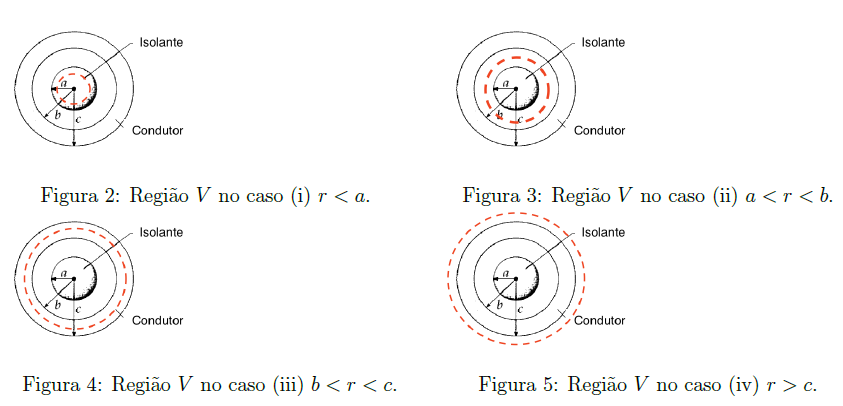
\includegraphics[scale=1]{eletromag-img/imagens.png}
  \caption{figuras}\label{figuraspng}
\end{figure}

b) Ache a carga induzida por unidade de área nas superfícies interna e externa do condutor.

\resposta Em todo condutor em equilíbrio eletrostático, a carga líquida se distribui na sua superfície. Vamos denotar por $q_{1}$ a carga induzida na superfície interna do condutor ($r = b$) e $q_{2}$ a carga induzida na superfície externa do condutor ($r = c$). Como dentro do condutor temos $E = 0$, aplicando a Eq. (\ref{eq9}) a uma região como as do item (a)(iii) (raio $r$, tal que $b < r < c$), a carga total em $V$ nesse caso é nula. Portanto,
%
\begin{equation}
  q_{V} = Q + q_{1} = 0 \ \ \ q_{1} = - Q .
\end{equation}
%
Como, por simetria, a carga se distribui de maneira uniforme na superfície, segue que a densidade de carga induzida em $r = b$ é
%
\begin{equation}
  \sigma_{1} = - \frac{Q}{ 4 \pi b^{2} } .
\end{equation}
%
Como o condutor está descarregado, por conservação de carga, temos que
%
\begin{equation}
  \begin{array}{ccc}
    Q_{condutor} & = & q_{1} + q_{2} \\
    q_{2} & = & - q_{1}
  \end{array}
\end{equation}
%
Usando novamente que, por simetria, a carga se distribui de maneira uniforme na superfície, a densidade de carga induzida em $r = c$ é
\begin{equation}
  \sigma_{2} = \frac{Q}{4 \pi c^{2}} .
\end{equation}



c) Esboce o gráfico da magnitude do campo elétrico $E$ versus $r$. Identifique em seu gráfico cada uma das regiões citadas no item (a).

\resposta Esboço do gráfico $E \times r$:
%
\begin{figure}[H]
  \centering
  \includegraphics[scale=1]{eletromag-img/esboco.png}
  \caption{Esboço do gráfico $E \times r$.}\label{esbocopng}
\end{figure}
%





\item Considere as equações de Maxwell na forma diferencial e resolva cada item abaixo.


a) Derive, mostrando todos os passos, as equações de onda no vácuo em sua forma vetorial para os campos elétrico e magnético. Lembre-se:
$$
\boldsymbol{ \nabla \times (\nabla \times V) = \nabla ( \nabla \cdot V ) - \nabla^{2} V } \mbox{ e  } \boldsymbol{ \nabla \cdot (\nabla \times V) = 0}
$$

\resposta Pelo formulário podemos ver que no vácuo (onde $\rho = 0$ e $\vec{J} = 0$), as equações de Maxwell são dadas por
%
\begin{eqnarray}
% \nonumber % Remove numbering (before each equation)
  \nabla \cdot \vec{E} &=& 0; \label{eq10} \\
  \nabla \cdot \vec{B} &=& 0; \label{eq11} \\
  \nabla \times \vec{E} &=& - \frac{\partial \vec{B}}{\partial t}; \label{eq12} \\
  \nabla \times \vec{B} &=& - \mu_{o} \epsilon_{o} \frac{\partial \vec{E}}{\partial t} . \label{eq13}
\end{eqnarray}
%
Tomando o rotacional da Eq. (\ref{eq12}) temos que
%
\begin{equation}\label{eq14}
  \nabla \times (\nabla \times \vec{E}) + \nabla \times \left( \frac{\partial \vec{B}}{\partial t}  \right) = 0 .
\end{equation}
%
Utilizando a primeira identidade vetorial dada no enunciado juntamente com a Eq. (\ref{eq10}), podemos re-escrever o primeiro termo do lado esquerdo da equação acima como
%
\begin{equation}
  \nabla \times (\nabla \times \vec{E}) = \nabla (\nabla \cdot \vec{E}) - \nabla^{2} \vec{E} = - \nabla^{2} \vec{E} .
\end{equation}
%
Desta forma a Eq. (\ref{eq14}) pode ser re-escrita, trocando a ordem das derivadas parciais, como
%
\begin{equation}
  -  \nabla^{2} \vec{E} + \frac{\partial}{\partial t} (\nabla \times \vec{B}) = 0 .
\end{equation}
%
Utilizando a Eq. (\ref{eq13}) obtemos a equação da onda para o campo elétrico
%
\begin{equation}
  \nabla^{2} \vec{E} = \mu_{o} \epsilon_{o} \frac{\partial^{2} \vec{E}}{\partial t^{2}} .
\end{equation}
%
Tomando agora o rotacional da Eq. (\ref{eq13}) temos que
%
\begin{equation}
  \nabla \times (\times \times \vec{B}) - \mu_{o} \epsilon_{o} \nabla \times \left( \frac{\partial \vec{E} }{\partial t}  \right) = 0 .
\end{equation}
%
Utilizando a primeira identidade vetorial dada no enunciado juntamente com a Eq. (\ref{eq11}) e trocando a ordem das derivadas parciais, podemos re-escrever a equação acima como
%
\begin{equation}\label{eq15}
  - \nabla^{2} \vec{B} - \mu_{o} \epsilon_{o} \frac{\partial}{\partial t} (\nabla \times \vec{E}) = 0 .
\end{equation}
%
Finalmente, utilizando a Eq. (\ref{eq12}) no segundo termo da Eq. (\ref{eq15}) obtemos
%
\begin{equation}
  \nabla^{2} \vec{B} = \mu_{o} \epsilon_{o} \frac{\partial^{2} \vec{B}}{\partial t^{2}} .
\end{equation}
%


b) Escreva a equação de onda para uma função escalar qualquer $f(\vec{r},t)$ e, comparando com as expressões obtidas no item (a), determine a velocidade de propagação para ambos os campos.

\resposta A equação de onda para uma função $f(\vec{r},t)$ se propagando com velocidade $v$ é dada por
%
\begin{equation}\label{eq16}
  \nabla^{2} f (\vec{r},t) = \frac{1}{v^{2}} \frac{\partial^{2} f (\vec{r},t) }{\partial t^{2}} .
\end{equation}
%
Comparando com as Eqs. (\ref{eq15}) e (\ref{eq16}), notamos que a velocidade de propagação de $\vec{E}$ e $\vec{B}$ é dada por
%
\begin{equation}\label{eq17}
  \frac{1}{v^{2}} = \mu_{o} \epsilon_{o} \Rightarrow \ \  v  = \frac{1}{\sqrt{\mu_{o} \epsilon_{o} }} = c.
\end{equation}
%



c) Uma possível solução da equação obtida no item (a) é a solução do tipo onda plana linearmente polarizada. Suponha um campo eletromagnético do tipo onda plana linearmente polarizada que esteja se propagando na direção $\hat{z}$. Considerando que $\omega$ é a frequência angular, $k$ o número de onda, $E_{0}$ e $B_{0}$ as amplitudes dos campos elétrico e magnético, respectivamente, escreva explicitamente qual é o módulo e a direção de $\vec{E}$ e $\vec{B}$ em função da posição e do tempo.

\resposta Supondo que $\vec{E}$ aponte na direção $\hat{x}$ e se propague na direção $\hat{z}$, podemos escrever que
%
\begin{equation}
\begin{array}{ccc}
  \vec{E} &=& E_{o} e^{i (kz - \omega t)} \hat{x} , \\
  \vec{B} &=& B_{o} e^{i(kz - \omega t)} \hat{y} \label{eq19} .  
\end{array}
\end{equation}
%
Os campos "físicos" podem ser escritos como (supondo $E_{o}$ e $B_{o}$ reais)
%
\begin{equation}
\begin{array}{ccc}
  \vec{E} &=& Re(\vec{E}) = E_{o} \cos (kz - \omega t) \hat{x} , \\
  \vec{B} &=& Re(\vec{B}) = B_{o} \cos (kz - \omega t) \hat{y} . \label{eq21} .
\end{array}
\end{equation}
%
Essas soluções, de fato, satisfazem as quatro Eqs. (10-13) desde que $ \omega = c k$, como pode ser verificado. De maneira geral, a direção de $\vec{E}$ é arbitrária, desde que seja perpendicular a $\vec{z}$. Uma vez fixada a direção de $\vec{E}$, $\vec{B}$ tem que ser perpendicular a $\vec{E}$ e $\vec{z}$. Os módulos de $\vec{E}$ e $\vec{B}$ são:
%
\begin{equation}
\begin{array}{ccc}
  E & = & E_{o} \cos(kz - \omega t), \\
  B & = & B_{o} \cos(kz - \omega t) .
\end{array}
\end{equation}
%

d) Partindo agora das equações de Maxwell na presença de cargas e correntes, derive a equação que relaciona as densidades de carga e de corrente elétrica (equação da continuidade). Que lei de conservação é expressa matematicamente por esta equação?


\resposta Tomando a divergência da Eq. (\ref{eq13}) temos
%
\begin{equation}\label{eq22}
  \nabla \cdot (\nabla \times \vec{B}) - \mu_{o} \epsilon_{o} \frac{\partial}{\partial t} (\nabla \cdot \vec{E}) = \mu_{o} \nabla \cdot \vec{J} .
\end{equation}
%
O primeiro termo se anula pela segunda identidade dada no enunciado. Usando a Eq. (\ref{eq10})
%
\begin{equation}
  \frac{\partial \rho}{\partial t} + \nabla \cdot \vec{J} = 0
\end{equation}

Esta equação expressa a lei de \textit{conservação da carga}: em sua forma integral, ela implica que a taxa de variação temporal da carga total incluída em uma região espacial fixa é igual ao fluxo de corrente elétrica entrando pela superfície que delimita a região.



\item {a)} Um cilíndrico dielétrico maciço, de comprimento infinito e raio $a$, possui uma densidade de carga volumétrica uniforme e positiva $\rho$. Uma casca cilíndrica, também dielétrica, de raio $b > a$, com eixo comum ao cilindro, tem uma densidade de carga superficial uniforme e negativa $\sigma$, de forma que a carga total do cilidro mais casca, em certo comprimento, é zero, e portanto $ \sigma = -\rho a^{2} / 2b$. Calcule o campo elétrico $\vec{E}(r)$ para as regiões $r < a$, $a < r < b$ e $b < r$ sendo $r$ a distância ao eixo do cilindro.


\resposta

b) Considere em seguida que o conjunto cilindro mais casca se move para a direita com velocidade $\vec{v}$. O movimento dá origem a uma corrente elétrica $I = \pi a^{2} \rho v$ no cilindro maciço, para a direita e uniformemente distribuida na seção reta, de forma que a densidade de corrente fica sendo dada por $\vec{J} = \rho \vec{v}$. Da mesma forma, a casca em movimento dá origem a uma corrente de mesma intensidade $I$, mas em sentido contrário (para a esquerda). Calcule a indução magnética $\vec{B}$ para as regiões $r < a$, $a < r < b$ e $b < r$.


\begin{figure}[H]
\centering
\includegraphics[scale=1]{eletromag-img/inducao.png}
\end{figure}



\item O campo elétrico de uma onda plana monocromática no vácuo é dado por

$$
\vec{E}(z,t) = ( E_{1} \hat{x} + E_{2} \hat{y} )e^{i(kz - \omega t)}.
$$
onde $\hat{x}$ e $\hat{y}$ são versores cartesianos nas direções $x$ e $y$, respectivamente, e $E_{1}$ e $E_{2}$ sáo constantes.


a) Encontre a indução magnética $\vec{B}(z,t)$.

\resposta

b) Mostre que o campo elétrico e a indução magnética são ortogonais entre si.

\resposta

c) Encontre o vetor de Poynting da onda.

\resposta


\item Uma espira condutora retangular (comprimento $a$, largura $b$ e resistência $R$) situa-se nas vizinhanças de um fio reto infinitamente longo que é percorrido por uma corrente $i$ para a direita, conforme a figura. A espira afasta-se do fio com uma velocidade constante $\vec{v}$, de forma que a distância do centro da espira ao fio é dada por $s(t) = s_{0} + vt$. Calcule:


a) o módulo do campo magnético produzido pela corrente num ponto situado a uma distância $r$ do fio. Indique a direção e o sentido do campo na região delimitada pela espira;

\resposta

b) o fluxo magnético na região delimitada pela espira para um dado valor de $s(t)$;

\resposta

c) a força eletromotriz induzida na espira para uma certa distância $s(t)$;

\resposta

d) a corrente induzida na espira, $i_{ind}$. Indique o sentido da mesma.

\begin{figure}[H]
\centering
\includegraphics[scale=1]{eletromag-img/espira2.png}
\end{figure}


\resposta


\item Um meio condutor tem condutividade elétrica $\sigma$, permeabilidade magnética $\mu_{0}$ e permissividade elétrica $\epsilon = K \epsilon_{0}$, em que $K$ é a constante dielétrica real. A equação de onda para o campo elétrico neste meio é dada por $\nabla^{2} \vec{E} - K \frac{1}{c^{2}} \frac{\partial^{2} \vec{E}}{\partial t^{2}} -  \frac{\sigma}{\epsilon_{0}} \frac{1}{c^{2}} \frac{\partial \vec{E}}{\partial t} = 0$, sendo $\frac{1}{c^{2}} = \mu_{0} \epsilon_{0}$.


a) Mostre que a função de onda plana monocromática $\vec{E}(z,t) = \vec{E_{0}}e^{i(\omega t - \tilde{q} z)}$ é solução da equação diferencial acima. Encontre a relação entre o número de onda complexo, $\tilde{q}$, e a frequência angular, $\omega$, para que $\vec{E}(z,t)$ seja solução. Mostre também que $\tilde{q}$ se torna real no caso de um meio isolante.

\resposta

b) Encontre a constante dielétrica complexa, $\tilde{K}$, usando a relação entre o número de onda e a constante dielétrica, $\tilde{q}^{2} = \tilde{K} \frac{\omega^{2}}{c^{2}}$. Verifique que a parte real de $\tilde{K}$ é igual a $K$ , como esperado, e explicite a parte imaginária de $\tilde{K}$.

\resposta

c) Faça a aproximação para baixas frequências na expressão da constante dielétrica complexa do item (b) e calcule o índice de refração complexo, $\tilde{n} = \sqrt{\tilde{K}}$. Mostre que as partes real e imaginária de $\tilde{n}$ são iguais neste caso.

\resposta

d) A profundidade de penetração da onda no meio condutor, $\delta$, é dada pelo inverso da parte imaginária do número de onda, $q_{i}$, ou seja, $\delta = 1/q_{i}$. Lembre-se de que $\tilde{q} = \tilde{n} \frac{\omega}{c}$ e calcule a profundidade de penetração para a prata ($Ag$) na região de micro-ondas ($f = \frac{\omega}{2\pi} = 10 GHz$), para a qual vale a aproximação do item (c). A condutividade da prata nesta faixa de frequências é $ \sigma_{Ag} = 3 \times 10^{+7}(\Omega m)^{-1}$. Aproxime o resultado do cálculo e obtenha a ordem de grandeza de $\delta_{Ag} (1 m, 10 cm, 1 cm ...)$.



\item Considere um condutor macroscópico de forma arbitrária, cuja superfície é fechada e suave. Partindo da lei de Gauss e considerando que o rotacional do campo eletrostático é nulo:


a) Calcule o campo elétrico no interior do condutor;

\resposta

b) Obtenha a componente normal do campo elétrico na superfície externa do condutor em termos da densidade superficial de carga;

\resposta

c) Obtenha a componente tangencial do campo elétrico na superfície do condutor.

\resposta



\item Considere um conjunto de soluções de ondas planas eletromagnéticas no vácuo, cujos campos (elétrico e magnético) são descritos pela parte real de funções: $\vec{u}(\vec{x},t) = \vec{A}e^{i(\vec{k} \cdot \vec{x} - \omega t)}$, onde $\vec{k}$ é o vetor de onda, que determina a direção de propagação da onda, e $\omega$ é a frequência angular, que se relaciona com o vetor de onda por $\omega = v |\vec{k}|$, onde $v = 1 / \sqrt{\epsilon \mu}$ é a velocidade de propagação das ondas.


a) Mostre que o divergente de $\vec{u}(\vec{x},t)$ satisfaz: $\vec{\nabla} \cdot \vec{u} = i \vec{k} \cdot \vec{u}$;

\resposta

b) Mostre que o rotacional de $\vec{u}(\vec{x},t)$ satisfaz: $\vec{\nabla} \times \vec{u} = i \vec{k} \times \vec{u}$;

\resposta

c) Demonstre que as ondas são transversais e que os vetores $\vec{E}$ , $\vec{B}$ e $\vec{k}$ são mutuamente perpendiculares.

\resposta



\item Um capacitor esférico é composto por uma esfera condutora de raio $R_{1}$, concêntrica com uma casca condutora esférica de raio $R_{2}$ e espessura desprezível, com $R_{1} < R_{2}$. O condutor interno possui carga $+Q$ e o externo possui carga $-Q$.


a) Calcule o campo elétrico e a densidade de energia em função de $r$, onde $r$ é a distância radial a partir do centro dos condutores, para qualquer $r$.

\resposta

b) Determine a capacitância $C$ do capacitor.

\resposta

c) Calcule a energia do campo elétrico armazenada em uma casca esférica de raio $r$, espessura $dr$ e volume $4\pi r^{2}dr$, localizada entre os condutores. Integre a expressão obtida para encontrar a energia total armazenada entre os condutores. Dê sua resposta em termos da carga $Q$ e da capacitância $C$.

\resposta


\item Duas bobinas idênticas, compostas cada uma por um anel de raio $R$ e espessura desprezível, são montadas com seus eixos coincidentes com o eixo$-z$, conforme se vê na figura abaixo. Seus centros estão separados por uma distância $d$, com o ponto médio P coincidindo com a origem do eixo$-z$. Cada bobina transporta uma corrente elétrica total de intensidade I. Ambas as correntes têm o mesmo sentido anti-horário.


a) Utilize a lei de Biot-Savart para determinar o campo magnético de uma única bobina ao longo de seu eixo de simetria.

\resposta

b) A partir do resultado anterior, obtenha o campo magnético $B(z)$ ao longo do eixo$-z$ das duas bobinas.

\resposta

c) Admitindo que o espaçamento $d$ seja igual ao raio $R$ das bobinas, mostre que, no ponto $P$, as seguintes igualdades são válidas: $dB/dz = 0$ e $d^{2}B/dz^{2} = 0$.

\resposta

d) Considerando os gráficos abaixo, de $B$ (em unidades arbitrárias) versus $z$, qual curva descreve o campo magnético ao longo do eixo$-z$ na configuração do item (b)? Justifique.

\resposta

e) Supondo que a corrente na bobina superior tenha seu sentido invertido, calcule o novo valor do campo magnético no ponto P.

\begin{figure}[H]
\centering
\includegraphics[scale=0.8]{eletromag-img/espira3.png}
\end{figure}

\resposta



\item Considere uma esfera sólida, uniformemente carregada, de carga $Q$ e raio $R$.


a) Determine o vetor campo elétrico $\vec{E}$ em um ponto à distância $r$ do centro da esfera, nos casos $r > R$ e $r \leq R$.

\resposta

b) Obtenha a força $d \vec{F}$ sobre um elemento de volume $dV$ da esfera, localizado na posição $\vec{r}$.

\resposta

c) Determine agora, por integração, a força total $\vec{F}$ que age sobre o hemisfério superior da esfera.

\resposta



\item Um capacitor de placas planas paralelas é formado por dois discos circulares de raio $a$, separados entre si de uma distância $d << a$, no vácuo. As placas estão ligadas a um gerador de corrente alternada de frequência $\omega$, que produz uma carga uniforme na placa do capacitor, dada por $q(t) = q_{0} sin(\omega t)$. São desprezados efeitos de borda. Supondo baixas frequências, de forma que $\omega a/c << 1$ (onde $c = 1/\sqrt{\mu_{0} \epsilon}$ é a velocidade da luz), o campo elétrico $\vec{E}$ entre as placas pode ser considerado uniforme. Considere um sistema de coordenadas cilíndricas, ($r,\theta,z$), com eixo $z$ passando pelo centro das placas, conforme indicado na figura.

\begin{figure}[H]
\centering
\includegraphics[scale=0.8]{eletromag-img/paralela.png}
\end{figure}


a) Calcule a expressão para o campo elétrico $\vec{E}$ entre as placas.

\resposta

b) Calcule o campo magnético $\vec{B}$, em função do raio $r$, na região entre as placas do capacitor.

\resposta

c) Calcule o vetor de Poynting $\vec{S} = (\vec{E} \times \vec{B} )/\mu_{0}$.

\resposta

d) Usando a aproximação de baixas frequências, mostre que é satisfeita a conservação de energia, expressa pela condição $\Delta \cdot \vec{S} + \partial u / \partial t = 0 $, onde $u = \frac{1}{2} ( \epsilon_{0} \vec{E}^{2} + \vec{B}^{2}/\mu_{0} )$ é a densidade de energia contida no campo eletromagnético.

\resposta


\item Considere um fio infinitamente longo disposto paralelamente ao eixo $z$, interceptando o plano $z = 0$ em $x = a$ e $y = 0$, conforme mostra a figura. O fio está carregado com densidade linear de carga elétrica $\lambda$ uniforme.

\begin{figure}[H]
\centering
\includegraphics[scale=0.8]{eletromag-img/fio.png}
\end{figure}


a) Determine o potencial elétrico $V (x,y,z)$ em todo o espaço, de forma que o potencial seja zero no eixo $z$. Sugestão: pode-se calcular o potencial a partir do campo elétrico do fio longo, que é obtido de forma simples usando a lei de Gauss.

\resposta

b) Considere agora, além do fio, um condutor plano infinito (aterrado) ocupando o plano $x = 0$. Calcule $V (x,y,z)$ para a região $x > 0$ do espaço. Sugestão: utilize o método das imagens.

\resposta

c) Qual a densidade superficial de carga $\sigma(y,z)$ induzida no condutor plano em $x = 0$?

\resposta

d) Calcule a integral $\int_{-\infty}^{\infty} \sigma (y,z) dy$ e discuta o resultado obtido.

\resposta



\item Um fio carregado com densidade linear de carga elétrica $\lambda > 0$ está colado (formando um anel) na borda de um disco isolante de raio $a$, que pode girar ao redor de seu eixo vertical sem atrito. O comprimento do fio é exatamente $2\pi a$. Apenas na região central do disco, até um raio $b < a$, age um campo magnético uniforme $\mathbf{B_{0}}$ vertical para cima.

\begin{figure}[H]
\centering
\includegraphics[scale=0.8]{eletromag-img/fio1.png}
\end{figure}


a) O campo magnético é agora desligado. Obtenha a expressão para o torque devido à força eletromotriz induzida no fio, em termos da variação temporal do campo magnético, $d\mathbf{B}/dt$. A partir deste resultado, calcule o momento angular final do disco (módulo e direção).

\resposta

b) Considerando como dado o momento de inércia $I$ do sistema disco$+$fio, calcule o campo magnético (módulo e direção) produzido no centro do disco pelo anel de carga na situação final acima.

\resposta


\item Um cabo coaxial é composto por um longo cilindro reto condutor de raio $a$ e uma fina casca cilíndrica condutora de raio $b$ e concêntrica ao cabo interno. Os dois condutores transportam correntes iguais e opostas de intensidade $i$.


a) Determine o módulo do campo magnético na região entre os dois condutores ($a < r < b$).

\resposta

b) Determine o módulo do campo magnético na região externa ao cabo coaxial ($r > b$).

\resposta

c) Encontre o módulo do campo magnético no interior do cilindro interno ($r < a$) se a corrente está distribuída uniformemente na seção transversal do mesmo.

\resposta

d) Calcule a energia armazenada no campo magnético por unidade de comprimento do cabo.

\resposta


\item Um capacitor esférico isolado possui carga $+Q$ sobre o condutor interno (raio ra) e carga $-Q$ sobre o condutor externo (raio $r_{b}$). A seguir, a metade inferior do volume entre os dois condutores é preenchida por um líquido de constante dielétrica relativa $K$, conforme indicado na seção reta da figura abaixo.

a) Calcule o módulo do campo elétrico no volume entre os dois condutores em função da distância $r$ ao centro do capacitor. Forneça respostas para a metade superior e para a metade inferior desse volume.

\resposta

b) Determine a densidade superficial de cargas livres sobre o condutor interno e sobre o condutor externo.

\resposta

c) Calcule a densidade superficial de cargas de polarização sobre as superfícies interna ($r_{a}$) e externa ($r_{b}$) do dielétrico.

\resposta

d) Qual é a densidade de carga de polarização sobre a superfície plana do dielétrico? Explique.

\resposta

e) Determine a capacitância do sistema.
\begin{figure}[H]
\centering
\includegraphics[scale=0.8]{eletromag-img/espira4.png}
\end{figure}

\resposta


\item Um cilindro de altura $h$ e raio externo $b$ é feito de um material com condutividade elétrica $\sigma$ e permissividade elétrica $\epsilon$. O cilindro é furado ao longo de seu eixo de forma que seu raio interno é $a$. Um material de alta condutividade elétrica preenche o furo central do cilindro e
forma também uma casca cilíndrica em torno da sua borda externa, formando os contatos elétricos do cilindro, conforme ilustra a figura abaixo. Considere $h >> b$, de modo que os efeitos de borda podem ser desprezados. Aplica-se uma diferença de potencial elétrico $V_{0}$ entre esses contatos (tome $V = 0$ na superfície externa do cilindro).



a) Mostre que, no regime estacionário ($\frac{\partial \rho}{\partial t} = 0$), a densidade de carga no interior do meio condutor homogêneo é nula.

\resposta

b) Mostre que, nesse caso, o potencial elétrico obedece à equação de Laplace e obtenha o vetor campo elétrico $\vec{E}(\vec{r})$ no interior do cilindro.

\resposta

c) Calcule a carga livre total acumulada na superfície do contato interno (raio $a$) e a capacitância entre os dois contatos elétricos.

\resposta

d) Calcule a resistência elétrica entre esses dois contatos elétricos.
\begin{figure}[H]
\centering
\includegraphics[scale=0.6]{eletromag-img/capacitor.png}
\end{figure}

\resposta



\item Um cilindro condutor muito longo de raio $a$ conduz uma corrente $I$ ao longo de seu eixo $z$. A densidade de corrente $\vec{J}$ no interior do cilindro varia de acordo com a expressão abaixo:
$$
\vec{J}(r, \varphi, z)=\hat{z} \frac{J_{0}}{r} \operatorname{sen}\left(\frac{\pi r}{a}\right)
$$
onde $r$ é a distância radial entre o ponto considerado e o eixo do cilindro.

a) Determine a constante $J_{0}$ em termos de $I$ e $a$.

\resposta

b) Calcule o campo magnético $\vec{B}$ fora do cilindro condutor ($r > a$) e expresse seu resultado em termos de $I$ e $a$.

\resposta


c) Calcule o campo magnético $\vec{B}$ no interior do cilindro condutor ($r < a$) e expresse seu resultado em termos de $I$ e $a$.

\resposta

d) Esboce um gráfico qualitativo do módulo do campo magnético, $B(r)$, indicando seu comportamento em $r = 0$ e $r = a$.

\resposta



\item Coloca-se uma esfera metálica descarregada, de raio $R$, numa região do espaço inicialmente preenchida por um campo elétrico dado por $\vec{E}_{i} = E_{0} \ \hat{k}$. Escolha a origem do sistema de coordenadas no centro da esfera.

a) Esboce as linhas do campo elétrico em toda a regi˜ao do espaço. Justifique o esboço utilizando argumentos físicos.

\resposta

b) Determine o campo elétrico $\vec{E}_{f} (\vec{r})$ em toda a região do espaço. Em particular, encontre os campos para os pontos em que $|\vec{r}| >> R$ e $|\vec{r}| >> R$ e verifique se eles s˜ao consistentes com o esboço no item (a).

\resposta

c) Ache a densidade de carga na esfera. Se a esfera possuir raio igual a $10 \ cm$ e $E_{0} = 100 \ N/C$, calcule as cargas acumuladas nos hemisférios norte e sul da esfera.

\resposta

d) Suponha que a esfera metálica seja substituída por uma esfera dielétrica. Discuta qualitativamente o que ocorre neste caso e esboce as linhas do campo elétrico em toda a região do espaço.

\resposta

\item Considere o arranjo hipotético ilustrado na figura abaixo, em que um fio sólido de raio $a$ estendido ao longo do eixo $z$ conduz uma corrente elétrica $I$, uniformemente distribuída sobre a sua seção transversal, que é mantida constante. A pequena lacuna no fio, de largura $w << a$, forma um capacitor de placas paralelas. A carga no capacitor é zero no instante $t = 0$.

a) Encontre o vetor campo elétrico na lacuna em função da distância $\rho$ a partir do eixo $z$ e do tempo $t$, além dos parâmetros $I$, $w$ e $a$. Despreze os efeitos de borda.

\resposta

b) Encontre o vetor campo magnético na lacuna em função de $\rho$ e $t$ e dos parâmetros $I$, $w$ e $a$.

\resposta

c) Calcule a densidade de energia eletromagnética $u_{em}$ e o vetor de Poynting na lacuna, indicando explicitamente a sua direção e o seu sentido.

\resposta

d) Determine a energia total $U_{em}$ na lacuna em função do tempo. Compare a taxa de variação de $U_{em}$ com o tempo e o fluxo de energia por unidade de tempo (fluxo de potência), obtido fazendo-se a integral de superfície do vetor de Poynting.

\begin{figure}[H]
\centering
\includegraphics[scale=0.8]{eletromag-img/solido.png}
\end{figure}

\resposta



\item Em uma fábrica de chocolate em pó, utiliza-se tubulações com ar comprimido para mover o chocolate em pó entre diferentes setores. Entretanto, com o atrito, o chocolate acaba ficando eletricamente carregado, de tal forma que temos uma densidade volumétrica uniforme de cargas positivas $\rho$ dentro da tubulação de raio $R$. Suponha que os tubos são condutores e encontram-se aterrados, e que a constante dielétrica do ar não é alterada pelo chocolate em pó.

a) Calcule o campo elétrico dentro e fora da tubulação, considerando que esta é um cilindro muito longo.

\resposta

b) Calcule o potencial elétrico dentro e fora da tubulação. Tome $V = 0$ na parede do tubo.

\resposta

c) Esboce o gráfico do campo elétrico e do potencial em função da distância ao eixo da tubulação.

\resposta

d) Se o campo elétrico for maior que um certo valor $E_{0}$, podemos ter o rompimento da rigidez dielétrica do ar, resultando numa faísca elétrica. Como o chocolate em pó é muito inflamável, uma faísca no interior da tubulação poderia causar uma explosão. Determine qual condição deve satisfazer para evitar este risco.

\resposta


\item Um plasma pode ser pensado como um gás clássico (não relativístico) de íons positivos e elétrons. Estamos interessados inicialmente na interação de uma onda eletromagnética com os elétrons livres deste plasma, já que estes têm massa muito menor do que os íons positivos.

a) Para uma onda eletromagnética harmônica transversal, seu campo elétrico $\vec{E}$ pode ser expresso na forma:
$$
\vec{E} = \vec{E}_{0} e^{i(\vec{k} \cdot \vec{r} - \omega t)}.
$$
Mostre que nas operações envolvendo $\vec{\nabla}$ este operador pode ser substituído por $i\vec{k}$, e as derivadas temporais $\frac{\partial}{\partial t}$ por $-i \omega$. Reescreva as equações de Maxell usando estes fatos.

\resposta

Considere que a onda harmônica se propaga na direção $z$ e suponha que o número médio de elétrons por unidade de volume do plasma é $n$.

b) Mostre que a densidade de corrente induzida pelo campo elétrico da onda é
$$
\vec{J} = i \frac{ne^{2}}{m \omega} \vec{E},
$$
onde $e$ e $m$ são, respectivamente, a carga e a massa do elétron, e $\omega$ é a frequência da onda. Justifique cuidadosamente suas hipóteses.

\resposta

c) Partindo das equações de Maxwell, obtenha a relação de dispersão $\omega(k)$ para a propagação da onda.

\resposta

d) O plasma admite a propagação de ondas com quaisquer frequências? Justifique sua resposta.

\resposta



\item Considere um fio infinitamente longo, carregado uniformemente com carga negativa de densidade $\lambda$, ao longo do eixo $x$. Suponha que acima deste fio, na posição $\vec{r} = y_{1} \hat{j}$, exista uma carga puntiforme $q$ positiva. O fio e a carga estão em repouso no referencial $S$. Um segundo referencial, $S'$, está se movendo para à direita, com uma velocidade relativística de módulo $v$, como mostra a figura abaixo. Tome a velocidade da luz como sendo $c$.
\begin{figure}[H]
\centering
\includegraphics[scale=0.8]{eletromag-img/fio2.png}
\end{figure}

a) Calcule a força resultante, $\vec{F}_{res}$, atuando na carga $q$ no referencial $S$.

\resposta

b) Encontre a densidade de carga $\lambda '$ no referencial $S'$. Note que nesse referencial, o fio carregado está em movimento, o que implica na existência de uma corrente elétrica. Calcule essa corrente, indicando o sentido dela.

\resposta

c) Qual a força resultante, $\vec{F}'_{res}$, no referencial $S'$? Compare com $\vec{F}_{res}$, obtida no item (a). Quais as direções e sentidos dessas duas forças?

\resposta

d) A relação entre as forças eletromagnéticas $\vec{F}_{res}$ e $\vec{F}'_{res}$, obtidas nos itens (a) e (c), são consistentes com os resultados da teoria da relatividade? Justifique a sua resposta. \textit{Dica}: Pela teoria da relatividade restrita, as transformações entre $\vec{F}_{\perp}$ e $\vec{F}'_{\perp}$ e entre $\vec{F}_{\parallel}$ e $\vec{F}'_{\parallel}$, onde $\perp$ e $\parallel$ indicam as direções perpendiculares e paralela ao eixo $x$ (direção do movimento de $S'$), respectivamente, podem ser obtidas sabendo-se que (i) a energia e momento ($E,\vec{p}$) nos referenciais $S$ e $S'$ se transformam como o tempo e espaço ($t,\vec{r}$) e que (ii) a segunda lei de Newton, $\vec{F} = d\vec{p}/dt$ é válida também na relatividade restrita. Faça a transformação somente na direção de $\vec{F}_{res}$ e $\vec{F}'_{res}$.




\item Um condutor esférico maciço, de raio $a$ e carregado com carga $Q > 0$, está envolto por um material dielétrico esférico, de constante dielétrica $\epsilon_{r} = \epsilon / \epsilon_{0}$ e raio externo $b$, conforme mostra a figura abaixo.
\begin{figure}[H]
\centering
\includegraphics[scale=0.8]{eletromag-img/esfera2.png}
\end{figure}
a) Determine o campo elétrico em todo o espaço e esboce um gráfico de seu módulo $E(r)$.

\resposta

b) Determine o potencial no centro das esferas, tomando-se como zero o potencial no infinito.

\resposta

c) Encontre as distribuições das cargas livre e ligada (de polarização) nas esferas condutora e dielétrica. Faça uma figura mostrando onde as densidades de cargas se localizam, indicando se são positivas ou negativas.

\resposta

d) Calcule a energia eletrostática do sistema.

\resposta


\item Um cabo coaxial é constituído por um fio sólido de raio $a$ envolto por uma casca cilíndrica concêntrica de raio $b$, com comprimento $L >> b$. Ele é usado como linha de transmissão entre uma bateria de $fem$ $V$ e uma resistência $R$, como indicado na figura abaixo. Despreze a resistência do cabo.

a) Calcule o vetor campo elétrico no interior do cabo coaxial ($a < r < b$).

\resposta

b) Calcule o vetor campo magnético no interior do cabo coaxial ($a < r < b$).

\resposta

c) Calcule o vetor de Poynting, indicando esquematicamente os vetores $\vec{E}$ , $\vec{B}$ e $\vec{S}$ com relação à seção transversal do cabo coaxial. O que aconteceria se os pólos da bateria fossem invertidos?

\resposta

d) Usando o vetor de Poynting, calcule a potência que flui da bateria para o resistor e explique por que este resultado é esperado. Observação: Indique claramente as superfícies gaussianas e/ou caminhos de integração utilizados nos cálculos acima.

\begin{figure}[H]
\centering
\includegraphics[scale=0.8]{eletromag-img/esfera2.png}
\end{figure}


\item Considere uma carga puntiforme $Q > 0$ a uma distância $D$ de uma placa infinita, condutora e aterrada, como ilustrada abaixo.

a) Desenhe as linhas de campo elétrico e as equipotenciais. Justifique seu desenho.

\resposta

b) Calcule as componentes $\hat{x}$ e $\hat{y}$ do vetor campo elétrico, em todo o espaço à esquerda da placa, em termos das componentes do ponto \textit{P} ilustrado na figura abaixo.

\resposta

c) Qual a densidade de carga na placa?

\resposta

d) Determine a força exercida pela placa sobre a carga \textit{Q}.

\begin{figure}[H]
\centering
\includegraphics[scale=0.8]{eletromag-img/placa.png}
\end{figure}

\resposta


\item Dois planos semi-infinitos, isolados entre si, estão posicionados angularmente em $\phi = 0$ e $\phi = \pi/6$, sendo que $V(\phi = 0) = 0$ e $V(\phi = \pi/6) = 100 V$.

a) Utilizando a equação de Laplace mostre que, região entre as duas placas (para $r>0$), o potencial eletrostático é dado por: $V = (600/\pi)\phi$.

\resposta

b) obtenha a expressão do vetor campo elétrico correspondente.

\resposta

c) Calcule a força sofrida por um elétron, quando colocado ($v_{0} = 0$) entre as duas placas. Descreva a trajetória do elétron; esta trajetória corresponde a um arco de circunferência? Justifique!

\begin{figure}[H]
\centering
\includegraphics[scale=0.8]{eletromag-img/placas.png}
\end{figure}

\resposta

\item Uma haste de cobre de massa $m$ é posicionada sobre trilhos condutores terminados por um segmento condutor com resistência $R$, conforme a figura. Paralelamente aos trilhos, existe um fio muito longo que é percorrido por uma corrente $I_{1}$. Suponha que em $t=0$ a haste é impulsionada com uma velocidade $v_{0}$ e deixada livre para mover-se, sem atrito.
\begin{figure}[H]
\centering
\includegraphics[scale=0.8]{eletromag-img/haste.png}
\end{figure}

a) Obtenha a expressão do campo magnético que atravessa a região da espira formada pela haste e os trilhos.

\resposta

b) Determine o sentido (horário/anti-horário) e o valor da corrente induzida na espira.

\resposta

c) Obtenha a expressão da velocidade da haste em função do tempo, em termos de $v_{0}$ e da constante $\tau$:
$$
\tau = \frac{4 \pi^{2} m R}{\mu_{0}^{2} I_{1}^{2} \operatorname{ln}^{2}(b/a)}
$$

\resposta


\item i) A partir das equações de Maxwell no vácuo:

a) Obtenha a equação de onda para o campo elétrico:
$$
\vec{\nabla}^{2} \vec{E} - \mu_{0} \epsilon_{0} \frac{\partial^{2} \vec{E}}{\partial t^{2}} = 0
$$

ii) Supor duas ondas eletromagnéticas planas, distintas, propagando-se na direção e sentido de $\hat{u}$ em um meio dielétrico com índice de refração $n=2$, com mesmas frequências e mesmos números de onda, que possuem respectivos campos elétricos dados por: $\vec{E}_{1} = E_{01} e^{-i(\omega t - K u)} \hat{p}$ e $\vec{E}_{2} = E_{02} e^{-i(\omega t - K u - \phi)} \hat{s}$.
\begin{figure}[H]
\centering
\includegraphics[scale=0.8]{eletromag-img/haste.png}
\end{figure}

\resposta

b) Discuta o estado de polarização de cada um destas ondas, em função dos possíveis valores da constante de fase $\phi$.

\resposta

c) Calcule o campo $\vec{B}$ e a média temporal do vetor de Poynting da onda resultante, correspondentes à superposição destas duas ondas.

\resposta


\item \textit{Experiência de Laboratório:} Um estudante decide medir a capacitância de um capacitor através de uma experiência calorimétrica. Ele aplica tensões variadas no capacitor, descarregando-o, logo em seguida, em um resistor $(R = 150 \Omega)$ mergulhado em um recipiente preenchido com óleo. Em cada etapa, o aumento de temperatura ocorrido no cunjunto óleo + resistor, após a descarga do capacitor, era cuidadosamente medida. Durante a execução de toda a experiência, o estudante também teve o cuidado de manter o conjunto (óleo e resistor, de Capacidade Térmica total $C_{T} = mc_{esp} = 200 J/ºC$) termicamente isolado do meio ambiente. A tabela de dados experimentais que ele obteve é mostrada abaixo.

\begin{center}
\begin{tabular}{|c|c|c|}
\hline
% after \\: \hline or \cline{col1-col2} \cline{col3-col4} ...
$\mathbf{V}[V]$ & $ \boldsymbol{\Delta T}[ºC] $ & $\boldsymbol{\sigma}_{\Delta T}[ºC]$ \\
50 & 0,1 & 0,1 \\ \hline
100 & 0,2 & 0,1 \\ \hline
150 & 0,3 & 0,1 \\ \hline
200 & 0,5 & 0,1 \\ \hline
250 & 0,6 & 0,1 \\ \hline
300 & 0,8 & 0,1 \\ \hline
350 & 1,1 & 0,1 \\ \hline
400 & 1,4 & 0,1 \\ \hline
450 & 1,7 & 0,1 \\ \hline
500 & 2,0 & 0,1 \\ \hline
\end{tabular}
\end{center}

a) Partindo do princípio de conservação de energia, mostre que a variação na temperatura do óleo é proporcional ao quadrado da tensão de carga dos capacitores: $\Delta T = \sigma V^{2}$; sendo $\alpha$ uma constante.

\resposta

b) Construa, no espaço quadriculado correspondente, um gráfico conveniente que lhe permite, a partir deste, obter o valor experimental da capacitância do capacitor utilizado pelo estudante na experiência.

\resposta

c) Como a experiência seria afetada caso o estudante resolvesse repetí-la utilizando um resistor do mesmo tipo só que com resistência $R' = 500 \Omega$? com qual destes resistores é possível realizar a experiência mais rapidamente?

\resposta


\item O betatron é um acelerador de elétrons, que se utiliza da força eletromotriz induzida por um campo magnético variável no tempo para acelerar os elétrons do feixe. Um campo magnético, também variável, serve para manter os elétrons em órbita circular. A figura 1 mostra um esquema do arranjo, visto de topo. Determine:
\begin{figure}[H]
\centering
\includegraphics[scale=0.8]{eletromag-img/eletromotriz.png}
\caption{Esquema de um betatron em vista de topo}
\end{figure}

a) A relação entre $B_{ind}$ e $B_{orb}$ para que os elétrons, ao serem acelerados, permaneçam na órbita desejada que a região de campo $B_{ind}$ vale para $r<R$;

\resposta

b) A energia máxima do feixe, em $MeV$, para o caso de uma órbita com $R = 0,1 m$ e $B_{orb} = 0,5 T$ (considere o elétron ultra-relativístico);

\resposta

c) O valor do campo elétrico a que os elétrons estão submetidos durante o processo de aceleração, supondo que o processo de subida do campo magnético demore 1 $ms$.

\resposta


\item Um laser de alta potência, como o que está sendo projetado no IPEN, é capaz de produzir um pulso de $0,1 J$, com duração de $0,1 ps$. Considere que a luz tenha comprimento de onda de $1 \mu m$, seja linearmente polarizada na direção $x$, que o feixe se propague na direção $z$ e que tenha seção reta circular com raio $R = 0,5 \ cm$.

a) Determine, para um pulso, a densidade média de energia e o fluxo médio d energia.

\resposta

b) Calcule a amplitude dos campos elétrico e magnético da onda eletromagnética.

\resposta

c) Calcule a pressão exercida por um pulso que incide sobre uma superfície perfeitamente refletora.

\resposta

d) Escreva as expressões correspondentes para os vetores $\vec{E}(z,t)$ e $\vec{B}(z,t)$.

\resposta



\item Explique, de maneira simples, o que é usualmente conhecido como \textit{poder das pontas}, ou seja, que, próximo a uma superfície condutora, o campo elétrico será tão mais intenso quanto menor for o raio de curvatura da superfície (Justifique sua resposta).


\item Quando perguntado pela irmã mais nova sobre o funcionamento de uma tela de computador, um estudante de física esboçou o esquema de um tubo de raios catódicos, como mostrado na figura 1.

\begin{figure}[H]
\centering
\includegraphics[scale=0.8]{eletromag-img/catodico.png}
\caption{Esquema de um tubo de raios catódicos}
\end{figure}

Explicou então a ela que os elétrons liberados pelo cátodo, a um potencial de $- kV$, são acelerados em direção ao ânodo, que, assim como o invólucro e a tela, está aterrado. Nessa situação os elétrons do feixe têm uma energia cinética de 1 $keV$. Ele também explicou o funcionamento das placas defletoras, que geram um campo elétrico vertical, o qual acelera os elétrons nessa direção, desviando-os da trajetória central. (Suponha que, para defletir o feixe para a extremidade da tela, as placas de deflexão tenham que ter uma $ddp$ de 10 $V$.) Afirmou, então, que os elétrons que chegam a uma das extremidades da tela têm uma energia cinética ligeiramente maior do que aqueles que chegam ao centro, por conta da aceleração experimentada entre as placas.

a) Que conceito(s) o estudante usou para fazer essa afirmação?

\resposta

b) Ele está correto? (Justifique suas resposta)

\resposta


\item Uma espira toroidal é mostrada na figura 2. Considere o enrolamento bem apertado, ou seja, que o campo magnético seja diferente de zero apenas no interior do toróide. Quando o meio em torno do qual a espira está enrolada é ferromagnético, a curva de $B \times H$ é mostrada na figura 3, iniciando com o material não magnetizado.

\begin{figure}[H]
\centering
\includegraphics[scale=0.8]{eletromag-img/toroide.png}
\caption{Curvas $B \times H$.}
\end{figure}
\begin{figure}[H]
\centering
\includegraphics[scale=0.8]{eletromag-img/toroide2.png}
\caption{Curvas $B \times H$.}
\end{figure}

a) Explique fisicamente as curvas indicadas por $a$, $b$ e $c$.

\resposta

b) Esboce a curva que seria observada (e explique) caso a bobina fosse enrolada em torno de um meio não magnético e não condutor.

\resposta


\item Um capacitor de placas planas, paralelas e circulares, com raios $a$ e separação $d$ ($d << a$), tem capacitância $C = \frac{\epsilon_{0} \pi a^{2}}{d}$. Ele é ligado a uma bateria que fornece tensão $V_{0}$, através de fios retilíneos muito longos, de resistência total $R$, que coincidem com o eixo $z$, como mostrado na figura abaixo. Supondo que a bateria seja ligado em $t=0 \ s$:

a) Monte a equação diferencial relacionando a carga do capacitor com os elementos do circuito e mostre que a corrente no circuito é dada por $I(t) = \frac{V_{0}}{R} \operatorname{exp} \left( - \frac{t}{RC}  \right)$.

\resposta

b) Determine o vetor $\vec{E}(\rho, \phi, z, t)$ no interior do capacitor (supondo-o em vácuo e desprezando efeitos de borda).

\resposta

c) Usando a lei de Ampère e considerando a corrente de deslocamento, determine o vetor $\vec{B}(\rho, \phi, z, t)$ no interior do capacitor.
\begin{figure}[H]
\centering
\includegraphics[scale=0.8]{eletromag-img/placaplana.png}
\caption{Circuito $RC$.}
\end{figure}

\resposta


\item O campo magnético de uma onda eletromagnética plana, no vácuo, é dado, em unidades do SI, por:
$$
\vec{B}(\vec{r}, t) = 10^{-6} (\hat{x} 2 \hat{y} + B_{z} \hat{z}) \operatorname{cos} (3x - y - z - \omega t)
$$
Determine:

a) A direção de propagação e o comprimento de onda.

\resposta

b) O valor da constante $B_{z}$.

\resposta


\item Um anel condutor de raio $R$ é colocado sobre o plano $xy$, centrado na origem. O campo magnético produzido por esse anel, ao longo do eixo $z$, quando por ele passa uma corrente $I$ no sentido $\phi$, é dado por:
$$
\vec{B}(z) = \frac{\mu_{0} I}{2} \frac{R^{2}}{ \left( R^{2} + Z^{2} \right)^{3/2}}
$$
A partir deste deste resultado, resolva o problema abaixo.

Considere agora um outro anel, de raio $a$, feito de material dielétrico e carregado uniformemente com carga $Q$. Esse anel está centrado na origem e tem um diâmetro ao longo do eixo $z$, em torno do qual é posto a girar com velocidade angular $\omega$ no sentido anti-horário ($\phi$), como mostrado na figura abaixo. Determine o vetor campo magnético na origem.

\begin{figure}[H]
\centering
\includegraphics[scale=0.8]{eletromag-img/anel2.png}
\caption{Espira que gira em torno de $z$.}
\end{figure}



\item Explique o efeito de atração de um ímã por um material não magnético e condutor demonstrado na sala. Sua explicação deve conter: $a)$ indicação do fenômeno eletromagnético responsável pelo efeito; e $b)$ influência do movimento do ímã.



\item Considere um anel isolante de raio $a$ com massa $M$ e carga total $Q$ uniformemente distribuídas. O anel repousa sobre um plano horizontal sobre o qual pode se mover livremente sem atrito. Na região do anel há um campo magnético devido a uma fonte externa dado por:

$$
\vec{B}(t) = \left\{
\begin{array}{cc}
B_{0} \hat{e}_{z}, & \mbox{ se } t < 0, \\
B_{0} \hat{e}_{z} e^{-\alpha t}, & \mbox{ se } t \geq 0,
\end{array}
\right.
$$

onde $B_{0}$ e $\alpha$ são constantes positivas. O plano em que repousa o anel é o plano $xy$ e o centro do anel coincide com a origem do sistema de coordenadas. No instante $t=0$ o anel encontra-se parado.

a) Determine o campo elétrico sobre o anel como função do tempo.

\resposta

b) Encontre a velocidade angular do anel num instante $t > 0$. Desconsidere o campo produzido pelo anel em movimento.

\resposta

c) Há conservação de momento angular neste processo? Explique.

\resposta


\item Uma placa condutora aterrada se encontra no plano $xy$ ($z=0$). Uma carga $q$ é trazida até o ponto $d\hat{e}_{z}$, com $d > 0$. Determine:

a) o potencial eletrostático em todo o espaço;

\resposta

b) o campo elétrico em todo o espaço;

\resposta

c) a densidade de carga e a carga total induzida na superfície do condutor;

\resposta

d) o trabalho realizado para trazer a carga $q$ do infinito até o ponto $d\hat{e}_{z}$.

\resposta



\item As propriedades eletromagnéticas da ionosfera terrestre podem ser descritas por uma permeabilidade magnética $\mu = \mu_{0}$ e uma constante dielétrica $\epsilon_{0}$ dependente da frequência (angular) $\omega$ na forma
$$
\epsilon(w) = \epsilon_{0} \left(  1 - \frac{\omega_{0}^{2}}{\omega^{2}}   \right)
$$
O parâmetro $\omega_{0}$ é determinado pela composição da ionosfera. Considere uma onda plana numa determinada região da ionosfera cujo campo elétrico é dado por
$$
\vec{E} = E_{0} e^{i(kz - \omega t)}.
$$

a) Obtenha a relação de dispersão $k(\omega)$.

\resposta

b) Para que valores de $\omega$ uma onda eletromagnética propaga neste meio?

\resposta

c) Qual a velocidade de fase $v_{f}$ de uma onda eletromagnética neste meio?

\resposta

d) É possível que $v_{f}$ seja maior que a velocidade da luz no vácuo $c$? Explique.

\resposta

e) Qual a velocidade de grupo $v_{g}$ desta onda? Esta velocidade pode ser maior que $c$?

\resposta


\item Considere um cabo coaxial formado por duas cascas cilíndricas condutoras de raios $a$ e $b$ ($b > a$). Um material de permeabilidade magnética $\mu$ ocupa o espaço entre as cascas cilíndricas, que são percorridas por uma corrente constante $I$ ao longo de seu comprimento como mostra a figura abaixo. Determine:

a) O campo $\vec{H}$ em todo espaço;

\resposta

b) o campo magnético $\vec{B}$ em todo espaço;

\resposta

c) a magnetização $M$ em todo espaço;

\resposta

d) as correntes de magnetização em todo o espaço;

\resposta

e) a energia armazenada no cabo por unidade de comprimento.

\begin{figure}[H]
\centering
\includegraphics[scale=0.7]{eletromag-img/coaxial2.png}
%\caption{Espira que gira em torno de $z$.}
\end{figure}

\resposta


\item Uma onda plana uniforme incide, do vácuo, em uma placa de vidro que possui índice de refração $n_{2}=1,5$. O campo elétrico desta onda é:
$$
\vec{E}_{i} = 4 \operatorname{cos} \left( 4,0 \pi  \times 10^{6} z - 1,2 \times 10^{15} t   \right)\hat{e}_{x}
$$
onde todas as grandezas são expressas no SI. As trajetórias dos raios luminosos correspondentes (incidente, refletido e transmitido) são mostradas na figura a baixo.
\begin{figure}[H]
\centering
\includegraphics[scale=0.7]{eletromag-img/vidro.png}
%\caption{Espira que gira em torno de $z$.}
\end{figure}

a) Transcreva a figura no seu caderno de resposta e, para cada onda, desenhe o campo magnético $\vec{B}$ e o vetor de onda $\vec{k}$ correspondentes (preocupe-se apenas com a direção e sentido dos vetores).

\resposta

b) Determine a velocidade de propagação, o comprimento de onda e a frequência das ondas incidente, refletida e transmitida.

\resposta

c) A partir de uma das equações de Maxwell determine o campo magnético da onda incidente e também o vetor de Poynting correspondente.

\resposta


\item Considere um capacitor plano, de placas paralelas muito grandes, no vácuo, com densidades de carga $+\sigma$ e $-\sigma$, que encontra-se em repouso no referencial do laboratório.

\begin{figure}[H]
\centering
\includegraphics[scale=0.7]{eletromag-img/placas2.png}
%\caption{Espira que gira em torno de $z$.}
\end{figure}

a) Qual é o campo elétrico e o campo magnético no interior do capacitor, medidos por um observador que encontra-se no referencial do laboratório (em repouso em relação ao capacitor)?

\resposta

b) Calcule os vetores campo elétrico e magnético no interior do capacitor, medidos por um observador que encontra-se em um referencial $S'$ (ver figura acima), movendo-se ao longo do eixo $x$ com velocidade $V$ constante.

\resposta

c) Supondo agora o observador movendo-se ao longo do eixo $z$ (perpendicularmente aos planos das placas), com velocidade constante $V$, calcule novamente os vetores campo elétrico e magnético no interior do capacitor.

\resposta


\item Em uma experiência de laboratório um estudante, para determinar a constante de tempo $\tau = RC$ de um capacitor comercial $C = 1,0 \mu F$, montou o circuito da figura abaixo, utilizando um resistor de 10 $M \Omega$ e uma pilha de $1,5 \ V$. Assim, quando a chave $S_{1}$ é fechada e a $S_{2}$ aberta, o capacitor é carregado até a máxima tensão. Em $t = 0 \ s$, a chave $S_{1}$ é aberta e a $S_{2}$ é fechada, descarregando o capacitor.
\begin{figure}[H]
\centering
\includegraphics[scale=0.7]{eletromag-img/circuito.png}
%\caption{Espira que gira em torno de $z$.}
\end{figure}

a) Para o processo de descarga, encontre a equação do circuito, resolvendo-a em $Q$, e mostre que $V = V_{0} \operatorname{exp}(-t/RC)$ corresponde à expressão que fornece a tensão no capacitor em função do tempo.

\resposta

b) Para realizar a medida de $\tau = RC$ o estudante optou por medir o tempo ($t_{1/2}$) que leva para que a tensão no capacitor seja exatamente a metade da tensão inicial. Para isto, ele utilizou um multímetro e um cronômetro manual. O procedimento foi realizado 10 vezes e os resultados estão representados na tabela abaixo.

\begin{tabular}{|c|c|c|c|c|c|c|c|c|c|c|}
\hline
% after \\: \hline or \cline{col1-col2} \cline{col3-col4} ...
$t_{1/2} \ (s)$ & 8,12 & 8,12 & 8,15 & 8,11 & 8,13 & 8,14 & 8,13 & 8,15 & 8,12 & 8,14 \\
\hline
\end{tabular}

\noindent Após calcular o valor médio utilizando uma calculadora, o estudante escreveu em seu relatório que $\langle t_{1/2} \rangle = 8,131 \pm 0,0137 \ s$. Você concorda com a forma com que ele expressou o valor o valor médio de $t_{1/2}$? Justifique. Se não concorda, como você expressaria o valor do tempo médio medido da maneira correta?

\resposta

c) A partir do valor arredondado de $t_{1/2} = 8 \ s$ (para uma rápida avaliação dos resultados), determine o valor experimental da constante de tempo $\tau_{exp}$ e compare com o seu valor nominal $\tau_{nominal}$.

\resposta

d) Construa um gráfico da tensão (eixo $y$) em função do tempo (eixo $x$) que represente a descarga do capacitor. Mostre neste gráfico, de uma maneira aproximada, os dados mais representativos da experiência ($V_{0}, \tau, t_{1/2}$).

\resposta



\item Considere uma distribuição esférica cargas, com densidade volumétrica de cargas constante, de raio $R_{e}$ e carga total $e$.

a) Determine o vetor campo elétrico $\vec{E}$ em todo o espaço (dentro e fora da distribuição esférica).

\resposta

b) Calcule a energia total associada a esta distribuição de cargas e mostre que:
$$
U = \frac{3}{5} \frac{e^{2}}{4 \pi \epsilon_{0} R_{e}}.
$$

\resposta

c) Supor que a energia calculada no ítem anterior corresponde à massa ($m_{e}$) de repouso do elétron. Calcule a expressão que fornece o raio do elétron e faça uma estimativa do seu valor, em metros.

\resposta



\item Considere um fio reto e infinito, pelo qual flui uma corrente $I$ constante. Calcule o vetor campo magnético $\vec{B}$ em um ponto $P$, à distância $\rho$ do fio:
\begin{figure}[H]
\centering
\includegraphics[scale=0.7]{eletromag-img/fio3.png}
%\caption{Espira que gira em torno de $z$.}
\end{figure}

a) utilizando a lei de Ampère:
$$
\oint \vec{B} \cdot d \vec{\ell} = \mu_{0} I;
$$

\resposta

b) utilizando a lei de Biot-Savart:
$$
d \vec{B} = \frac{\mu_{0} I}{4 \pi} \frac{d \vec{\ell} \times \hat{e}_{r}}{r^{2}}
$$

\resposta

c) através do cálculo do potencial vetor:
$$
\vec{A} =  \frac{\mu_{0}}{4 \pi} \int \frac{\vec{J} dV}{r}
$$
\item[  ] Lembre-se que $ \vec{J} dV \longleftrightarrow I d \vec{\ell} $.
\item[  ] Sugestão: Suponha um fio de comprimento $L$ muito grande, de forma que $L >> \rho$.

\resposta



\item Foi idealizado um experimento para o estudo da polarização de ondas eletromagnéticas por reflexão em uma superfície dielétrica plana. Uma onda não polarizada pode ser considerada como tendo componentes do campo elétrico paralela (componente $p$) e não paralela (componente $s$) à superfície do dielétrico, de forma que os coeficientes de Fresnel correspondentes são:
\begin{multicols}{2}
$$
r_{12p} = \frac{n_{1} \operatorname{cos} \theta_{1} - n_{2} \operatorname{cos} \theta_{2}}{n_{1} \operatorname{cos} \theta_{1} + n_{2} \operatorname{cos} \theta_{2}} = \frac{\operatorname{sen}( \theta_{2} - \theta_{1} )}{\operatorname{sen}( \theta_{2} - \theta_{1} )}; \\
$$

$$
r_{12p} = \frac{n_{1} \operatorname{cos} \theta_{1} - n_{2} \operatorname{cos} \theta_{2}}{n_{1} \operatorname{cos} \theta_{1} + n_{2} \operatorname{cos} \theta_{2}} =  \frac{\operatorname{tg}( \theta_{2} - \theta_{1} )}{\operatorname{tg}( \theta_{2} + \theta_{1} )}.\\
$$

\begin{figure}[H]
\centering
\includegraphics[scale=0.7]{eletromag-img/dieletrico2.png}
\end{figure}

\end{multicols}


a) Notando que a polarização ocorre quando $\theta_{1}$ ($\theta_{1} = \theta_{B}$) satisfaz a condição $\theta_{1} + \theta_{2} = \pi/2$, mostre que $\operatorname{tg} \theta_{B} = n_{2}/n_{1}$ e que, nesta condição, o coeficiente de Fresnel da componente da onda que não se anula pode ser escrito como:
$$
r_{12} = \frac{1 - n_{2}^{2}}{1 + n_{2}^{2}}.
$$

\resposta

b) No experimento, um painel de polietileno e um conjunto emissor/receptor de micro-ondas foi utilizado, conforme mostrado na figura a baixo.
\begin{figure}[H]
\centering
\includegraphics[scale=0.7]{eletromag-img/experimento.png}
\end{figure}
O ângulo de incidência foi sendo variado e as intensidades relativas $I_{p}/I_{0}$ e $I_{s}/I_{0}$ da onda correspondentes às componentes $p$ e $s$, foram registradas na tabela abaixo.

\begin{tabular}{|c|c|c|}
\hline
\multirow{2}{*}{Ângulo $(\theta_{1})$}
& \multicolumn{2}{c|}{Leituras dos medidores}   \\ \cline{2-3}
& $I_{s}/I_{0}$   & $I_{p}/I_{0} $              \\ \hline
20°              & $0,41 \pm 0,04$ & $0,36 \pm 0,04$             \\
25°              & $0,28 \pm 0,04$ & $0,34 \pm 0,04$             \\
30°              & $0,26 \pm 0,04$ & $0,28 \pm 0,04$             \\
35°              & $0,24 \pm 0,04$ & $0,21 \pm 0,04$             \\
40°              & $0,15 \pm 0,04$ & $0,19 \pm 0,04$             \\
45°              & $0,11 \pm 0,04$ & $0,20 \pm 0,04$             \\
\hline
\end{tabular}
\begin{tabular}{|c|c|c|}
\hline
\multirow{2}{*}{Ângulo $(\theta_{1})$}
& \multicolumn{2}{c|}{Leituras dos medidores}   \\ \cline{2-3}
& $I_{s}/I_{0}$   & $I_{p}/I_{0} $              \\ \hline
50°              & $0,10 \pm 0,04$ & $0,17 \pm 0,04$             \\
55°              & $0,05 \pm 0,04$ & $0,14 \pm 0,04$             \\
60°              & $0,03 \pm 0,04$ & $0,19 \pm 0,04$             \\
65°              & $0,04 \pm 0,04$ & $0,23 \pm 0,04$             \\
70°              & $0,19 \pm 0,04$ & $0,48 \pm 0,04$             \\
75°              & $0,44 \pm 0,04$ & $0,65 \pm 0,04$             \\
\hline
\end{tabular}

\item [  ]Com os dados da tabela construa o gráfico adequado e, a partir deste, determine o ângulo de Brewster $\theta_{B}$.

\resposta

c) Determine o índice de refração do painel de polietileno utilizado no experimento. Calcule a refletância $R$ da onda quando o ângulo de incidência da onda corresponde ao ângulo de Brewster e compare com o valor experimental.

\resposta

d) Como você relaciona este fenômeno de polarização com a utilização de óculos específicos por pessoas que vão à praia, que esquiam na neve, etc? Explique!

\resposta


\item Um cilindro muito longo de raio $R$ é fabricado com um material isolante cuja constante dielétrica é $K (= \epsilon / \epsilon_{0})$ e que possui uma densidade de carga livre cilindricamente simétrica, mas não uniforme $\rho(r)$.

a) Determine $\rho(r)$ tal que o campo elétrico dentro do cilindro seja radial apontando para fora do mesmo e com módulo constante $E_{0}$;

\resposta Usando como superfície um cilindro concêntrico de raio $r$ tal que este seja menor que $R$ e altura $h$, temos, pela lei de Gauss, ignorando o caráter finito do cilindro:
$$
\oint \vec{E} (\vec{r}) \cdot d \vec{S} = \frac{q_{int}}{e}
$$
utilizando $d\vec{S} = d A \hat{r}$, logo:
$$
\begin{array}{ccl}
  2 \pi r h |\vec{E}(\vec{r})| & = & \frac{1}{K \epsilon_{0}} \int_{0}^{r} \int_{0}^{h} \int_{0}^{2\pi} \rho (r') d^{3} r' \\
  & = & \frac{1}{K \epsilon_{0}} \int_{0}^{r} \int_{0}^{h} \int_{0}^{2\pi} \rho (r') r' d \theta' d z' d r' = \frac{2\pi h}{K \epsilon_{0}} \int_{0}^{r} \rho (r')r' d r' \\
  |\vec{E}(\vec{r})|  & = & \frac{1}{K \epsilon_{0} r} \int_{0}^{r} \rho(r') r' d r'
\end{array}
$$
Como desejamos que $\rho (\vec{r'}) = |\vec{E}| = E_{0}$, $\forall \ \epsilon \ [0, R]$, temos:
$$
|\vec{E}(\vec{r})| = E_{0} = \frac{1}{K \epsilon_{0} r} \int_{0}^{r} \rho (r') dr' \ \Rightarrow \ E_{0} K \epsilon_{0} r = \alpha r = \int_{0}^{r} \rho (r') r' dr'
$$
Sabemos que:
$$
\int_{0}^{r} \alpha d r' = \left. \alpha r' \right|_{0}^{r} = \alpha r
$$
Logo:
$$
 \rho (r') r' = \alpha \ \Rightarrow \ \rho (r') = \frac{\alpha}{r'} = \frac{E_{0} K \epsilon_{0}}{r'}
$$


b) para a densidade de carga determinada em (a), calcule o campo elétrico $\vec{E}(r)$ fora do cilindro;

\resposta Como a carga interna é:
$$
q_{int} = \int_{0}^{R} \int_{0}^{h} \int_{0}^{2\pi} \rho (r) r d \theta d z d r = 2 \pi h \int_{0}^{R} E_{0} K \epsilon_{0} d r' = \left.  2 \pi h E_{0} K \epsilon_{0} r \right|_{0}^{R} = 2 \pi h E_{0} K \epsilon_{0} R
$$
Usando como superfície um cilindro concêntrico de raio $r$ tal que este seja maior que $R$ e altura $h$, temos, pela lei de Gauss:
$$
\oint \vec{E} \vec{r} \cdot d \vec{S} = \frac{q_{int}}{\epsilon_{0}}
$$
Logo:
$$
\oint \vec{E} (\vec{r}) \cdot d \vec{S} = \frac{q_{int}}{\epsilon_{0}} \ \Rightarrow \ 2\pi h E_{0} K R = 2 \pi r h |\vec{E}(\vec{r})|
$$
Portanto, usando a simetria (adotando o sinal positivo  para a cargas positivas), sendo $\hat{r}$ o versor radial do cilindro, que aponta para fora deste:
$$
|\vec{E}(\vec{r})| = \frac{E_{0} K R}{r} \ \Rightarrow \ \vec{E}(\vec{r}) = \frac{E_{0} K R}{r} \hat{r}
$$



c) se o cilindro for então envolvido por uma casca cilíndrica condutora neutra de raio interno $a$ ($a > R$) e raio externo $b$ ($b > a$), concêtrica ao mesmo, determine as densidades de carga induzidas nas superfícies da casca condutora;

\resposta

Como os metais são condutores, o campo elétrico dentro deles deve ser nulo. Logo, ao efetuar uma lei de Gauss no interior do metal, sabemos que $\forall \ r \epsilon (a,b)$ deve valer:
$$
\oint \vec{E} \vec{r} \cdot d \vec{S} = 0 = \frac{q_{int}}{\epsilon_{0}} \Rightarrow q_{int} = 0
$$
Para que isso ocorra só há uma alternativa: deve haver uma carga de valor na superfície interna do metal, distribuída uniformemente ao longo da superfície interna do cilindro. Supondo que o metal seja eletricamente neutro, se efetuarmos outra lei de Gauss para $r > b$, notamos que a superfície externa do metal deve possuir carga $q_{int}$ também uniformemente distribuída, na superfície externa do cilindro. As densidades de carga serão, se for a altura do cilindro, com
$$
\lambda = \frac{q_{int}}{h}, \ \ \sigma_{a} = \frac{\lambda}{2 \pi a} \ \mbox{ e } \   \sigma_{b} = \frac{\lambda}{2 \pi b}.
$$


\item[] Se por densidade de carga entendermos densidade linear de carga, a superfície interna possui densidade de carga $-\lambda$ e a superfície externa possui densidade de carga $\lambda$.



\item[] Se por densidade de carga entendermos densidade superficial de carga, a superfície interna possui densidade de carga $-\sigma_{a}$ e a superfície externa possui densidade de carga $\sigma_{b}$.



d) para a situação do item (c), esboce um gráfico do módulo do campo elétrico $E(r)$ em função da distância ao eixo do cilindro, em todo o espaço.

\resposta

\begin{figure}[H]
\centering
\includegraphics[scale=0.7]{eletromag-img/campo.png}
\caption{Note que o gráfico é descontínuo devido às mudanças de meios (dielétrico 1 - dielétrico 2 - metal - dielétrico 2). Note que o campo dentro do metal é nulo, e dentro do dielétrico 1 é menor devido ao maior efeito de polarizabilidade das moléculas nesta região.}
\end{figure}



\item Uma barra metálica uniforme de massa $M$ pode deslizar com atrito desprezível ao longo de um par de trilhos horizontais fixos separados por uma distância $d$, conforme mostra a figura abaixo.

\begin{figure}[H]
\centering
\includegraphics[scale=0.7]{eletromag-img/barra.png}
\end{figure}

Os trilhos e a ligação transversal da esquerda são altamente condutores, de modo que suas contribuições para a resistência elétrica do circuito retangular são desprezíveis. A barra livre e os contatos com os trilhos fixos têm resistência elétrica total $R$. Há um campo magnético uniforme e estacionário aplicado externamente, de módulo $B$, orientado verticalmente e apontando para cima.

a) Determine a corrente $i$ induzida no circuito em termos de $d$, $R$, $B$ e $v$, a velocidade instantânea da barra. Considere como o sentido positivo da corrente na barra aquele indicado na figura. Ao determinar a corrente induzida, despreze o campo magnético produzido pela própria corrente;

\resposta

b) suponha que em $t = 0$ a barra esteja numa posição $x_{o}$ e com velocidade $v_{o}$. Determine $x(t)$ e $v(t)$;

\resposta

c) obtenha expressões numéricas para $x(t)$, $v(t)$ e $i(t)$ usando os seguintes parâmetros: $M = 0,10 kg$, $d = 1,0  m$, $R = 1,0 \Omega$, $B = 0,2 T$, $x_{0} = 3,0 m$ e $v_{0} = 10 m/s$. Qual a posição final da barra quando ela estiver em repouso?

\resposta

d) É justificável desprezar no item (a) o campo magnético produzido pela corrente induzida? Para responder esse item, calcule a razão entre o maior valor do campo magnético produzido pela corrente induzida ($B_{i}$) e o valor do campo aplicado ($B$). Estime $B_{i}$ calculando o campo magnético na superfície da barra livre, assumindo que ela é muito longa e tem seção transversal circular com raio $a = 3,0 mm$.

\resposta


\item No instante inicial $t = 0$, uma partícula de massa $m$ e carga $q$ encontra-se na posição $x_{0} \hat{x}$ e com velocidade $v_{0} \hat{y}$. Os campos de força agindo sobre a partícula são devidos somente ao potencial elétrico $\phi$ e ao potencial vetor $\vec{A}$, dados por
$$ \Phi (\vec{r}) = \alpha_{0} x + a \alpha_{1} ; $$
$$ \vec{A} (\vec{r}) = \frac{\beta_{0}}{2} ( \vec{z} \times \vec{r} ) +  a \beta_{1} \hat{u} e^{\hat{u} \cdot \vec{r} / a} ,$$
onde $\alpha_{0}$, $\alpha_{1}$, $a$, $\beta_{0}$ e $\beta_{1}$ são constantes reais e $\hat{u}$ é um versor constante e real.

a) Calcule o vetor campo elétrico em todo o espaço, $\vec{E}(\vec{r})$.

\resposta

b) Determine o vetor indução magnética em todo o espaço, $\vec{B}(\vec{r})$.

\resposta

c) Existe algum valor para a velocidade inicial $v_{0}$ tal que a trajetória da partícula seja uma reta? Em caso afirmativo, calcule-o.

\resposta



\item Durante uma tempestade, uma nuvem cobre a cidade de São Paulo a uma altura $h = 500 m$ em relação ao solo. Vamos supor que a largura da nuvem seja bem maior que essa altura $h$. Um balão meteorológico equipado com um sensor de campo elétrico é então lançado verticalmente a partir do solo. Os dados coletados pelo sensor estão ilustrados na figura abaixo, onde $E(z)$ é o módulo do campo elétrico em função da altitude ($z = 0$ no solo). A espessura da nuvem na direção vertical é igual a $1200 m$ e sabe-se que a densidade de carga elétrica é sempre negativa no seu interior.

\begin{figure}[H]
\centering
\includegraphics[scale=0.7]{eletromag-img/magnetico.png}
\end{figure}

a) Indique, em um diagrama, a direção e sentido do campo elétrico nas regiões abaixo, dentro e acima da nuvem.

\resposta

b) Calcule a densidade volumétrica de carga na atmosfera em função da altitude, $\rho(z)$, e esboce o seu gráfico.

\item[] Para quais valores de $z$ o potencial elétrico é máximo ou mínimo? Calcule o potencial elétrico nesses pontos? Tome $V = 0$ no solo.





\item Uma onda eletromagnética monocromática polarizada linearmente propagando-se ao longo da direção $+ \hat{x}$ é representada na notação complexa pelo campo elétrico $ \vec{E}(x,t) = \hat{y} E_{0} e^{i(kx - wt)} $. Considere que essa onda propaga-se no ar ($n_{ar} \approx 1$) e possui comprimento de onda $\lambda_{0} = 0,50 \mu m$ (luz verde) e intensidade $I_{0} = 10 W/m^{2}$.

a) Escreva uma expressão análoga à equação acima para o campo magnético $\vec{B}(x,t)$ dessa onda, escrevendo sua amplitude $B_{0}$ em função de $E_{0}$ no sistema SI de unidades.

\resposta

b) Essa onda incide perpendicularmente a uma placa de 1,0 $mm$ de espessura feita de um material que possui índice de refração $n = n_{R} + i n_{j}$, onde $n_{j} << n_{R}$ para ondas dessa frequência. Dada a expressão abaixo para a refletividade $R$ da interface entre o meio 1 (índice de refração $n_{1}$) e o meio 2 (índice de refração $n_{2}$), estime a partir do seguinte gráfico (intensidade I versus posição $x$) a parte real $n_{R}$ do índice de refração do material.

\resposta

c) Estime, também a partir do gráfico, a parte imaginária $n_{I}$ do índice de refração.

\resposta

d) Qual a frequência e o comprimento de onda da radiação dentro do material?

$$
R = \left| \frac{n_{1} - n_{2}}{n_{1} + n_{2}}   \right|^{2}
$$
\begin{figure}[H]
\centering
\includegraphics[scale=0.7]{eletromag-img/placa3.png}
\end{figure}

\resposta


\item Um solenoide circular é projetado com $81\pi \ mm^{2}$ de área de seção transversal e $40 \pi \ mm$ de comprimento. Desprezando os efeitos do comprimento finito do solenóide, responda:

a) Quantas voltas de fio são necessárias para que o módulo do campo magnético próximo ao centro do solenóide seja de 2,0 $mT$ quando percorrido por uma corrente de 1,0 $A$?

\resposta

b) Se o solenoide é enrolado compactamente (sem espaçamento entre voltas consecutivas) com uma única camada de fio de cobre de resistividade $2,0 \times 10^{-8} \ \Omega m$, qual é a resistência elétrica do solenoide? Despreze a espessura do isolante que recobre o fio.

\resposta

c) Que diferença de potencial deve ser aplicada nos terminais do solenóide para produzir o campo magnético de 2,0 $mT$?

\resposta

d) Para esse valor do campo, qual a energia magnética armazenada no solenoide?

\resposta

e) Determine a indutância desse solenóide.

\resposta



\item Uma placa metálica fina e carregada está imersa em uma solução aquosa de cloreto de sódio (sal de cozinha), cuja constante dielétrica é $K = \epsilon / \epsilon_{0} = 80$. Considere esta placa como infinita e situada no plano $xy$ de um sistema de coordenadas. Determinou-se que o potencial elétrico na solução nas vizinhanças da placa e dado pela seguinte expressão:
$$
V(x,y,z) = 10 \mathrm{exp}(-20|z|)
$$
com $z$ medido em metros e $V$ em volts.

a) Determine o vetor camp o elétrico correspondente a esse potencial.

\resposta

b) Qual a magnitude e sinal da densidade superficial de carga livre $\sigma(x,y)$ da placa?

\resposta

c) Determine a densidade volumétrica de carga livre $\rho(x,y,z)$ na solução, nas proximidades da placa.

\resposta


\item  O fio retilíneo muito longo da figura abaixo conduz uma corrente $i$ no sentido indicado, cuja magnitude está crescendo a uma taxa $\mathrm{d} i/\mathrm{dt}$.

a) Quando a corrente no fio é igual a $i$, calcule o fluxo magnético através da espira retangular.

\resposta

b) Obtenha uma expressão para a força eletromotriz induzida na espira.

\resposta

c) Se a resistência da espira é 0,051 $\Omega$, calcule o valor numérico da corrente induzida na espira e indique seu sentido para $a = 12 cm$, $b = 36 cm$, $L = 24 cm$ e$\mathrm{d} i/\mathrm{dt} = 9,6 \ A/s$.

\begin{figure}[H]
\centering
\includegraphics[scale=0.7]{eletromag-img/barrae.png}
\end{figure}

\resposta




\end{enumerate}








%
%
\chapter{Moderna}

\begin{enumerate}[start=1,label={\bfseries Q\arabic*.}]

\item Uma batalha espacial entre duas naves de civilizações diferentes, A e B, em repouso uma em relação à outra, acaba em destruição mútua. Um observador C, em repouso em relação às duas naves e para quem a distância entre elas era $L$, observa a nave da civilização A explodir um tempo $T$ antes da explosão da outra nave. Um outro observador D move-se com velocidade de magnitude $u$ em relação ao primeiro observador, ao longo da linha que separava as duas naves.


a) Supondo uma situação em que $L = 1.000 km$ e $u = \frac{24}{25}c$, sendo $c$ a velocidade da luz no vácuo, qual era a distância entre as naves no referencial do observador $D$?

    {\color{red}
    O observador $D$ observa um comprimento $L'$ relacionado a $L$ através da contração de Lorentz,

    $$
    L' = L \sqrt{1 - \frac{u^{2}}{c^{2}}}.
    $$

    Substituindo os valores do enunciado, $L' = 280 \ km$.


    }

b) Em outra situação, supondo $L = 1.000 km$ e $T = 1 ms$, qual deveria ser a magnitude mínima da velocidade $u$ para que o observador D registrasse a explos˜ao da nave da civilização B como tendo ocorrido antes da explosão da nave da civilização A?

    {\color{red}

    Supondo, sem perda de generalidade, que as naves situam-se ao longo do eixo $x/x'$ em ambos os referenciais de C e D, e que as origens destes coincidem no instante $t = t' = 0$, os referenciais relacionam-se pela transformação de Lorentz

    $$
    x^{\prime} = \gamma (x - ut) \quad \ \ \ t^{\prime} = \gamma \left( t - \frac{u}{c^{2}} x \right),
    $$

    com

    $$
    \gamma = \frac{1}{\sqrt{1-\frac{u^{2}}{c^{2}}}}
    $$

    Denotando por 1 e 2 as explosões das naves das civilizações A e B, respectivamente, temos


    \begin{eqnarray*}
    % \nonumber % Remove numbering (before each equation)
      \Delta x &=& x_{2} - x_{1} = L \quad \ \ \ \quad \Delta t = t_{2} - t_{1} = T, \\
      \Delta t' &=& t'_{2} - t'_{1} = \gamma \left(  \Delta t - \frac{u}{c^{2}} L \right).
    \end{eqnarray*}

    Para que o observador D registre o evento 2 como anterior ao evento 1, é preciso que

     $$
     \Delta t' < 0 \Rightarrow T - \frac{u}{c^{2}} L < 0,
     $$

    ou seja,

    $$
    u > \frac{c^{2}T}{L} = 9 \times 10^{4} km/s.
    $$

    }


c) Considere que toda a energia de repouso da nave da civilização A tenha sido liberada na explos˜ao e que o veículo do observador C tenha capturado toda essa energia, convertendo-a em energia cinética. Sendo iguais as massas da nave da civilização A e a do veículo de C, determine a velocidade $v$ que o veículo atinge após absorver a energia da explos˜ao.

{\color{red}

$$
m_{A} c^{2} = \frac{m_{C} c^{2}}{\sqrt{1-\frac{v^{2}}{c^{2}}}} - m_{C} c^{2}.
$$

Portanto,


$$
\begin{aligned}
& \sqrt{1-\frac{v^{2}}{c^{2}}}=\frac{m_{C}}{m_{A}+m_{C}} \Rightarrow \frac{v^{2}}{c^{2}} = 1-\left(\frac{m_{C}}{m_{A}+m_{C}}\right)^{2}\\
& v = c \sqrt{1 - \left(\frac{m_{C}}{m_{A}+m_{C}} \right)^{2}}
\end{aligned}
$$

com $m_{A} = m_{C}$, obtemos

$$
v = \sqrt{\frac{3}{4}}c.
$$

}








\item A superfície do Sol está a uma temperatura aproximada de $6,0 \times 10^{3} \ K$, enquanto a superfície da estrela supergigante Betelgeuse está a uma temperatura aproximada de $3,0 \times 10^{3} \ K$. Suponha que ambas as estrelas irradiem como corpos negros perfeitos.


  a) A radiância espectral é definida como a energia irradiada por unidade de tempo e por unidade de área da superfície de um corpo no intervalo de comprimentos de onda entre $\lambda$ e $\lambda + d\lambda$. Qual é a razão entre o comprimento de onda para o qual a radiância espectral do Sol é máxima e o comprimento de onda correspondente para Betelgeuse?

  {\color{red}

  Pela lei do deslocamento de Wien, o produto da temperatura de um corpo negro pelo comprimento de onda que maximiza sua radiância espectral é constante. Logo, para o Sol (S) e Betelgeuse (B) vale

$$
\lambda_{S} T_{S} = \lambda_{B} T_{B} \Rightarrow = \frac{\lambda_{S}}{\lambda_{B}} = \frac{T_{B}}{T_{S}} = \frac{3,0 \times 10^{3}}{3,0 \times 10^{3}} = \frac{1}{2}.
$$


  }


  b) Qual é a razão entre a radiância (energia total irradiada por unidade de tempo e de área da superfície) na superfície do Sol e a radiância na superfície de Betelgeuse?

  {\color{red}

Pela lei de Stefan-Boltzmann, a radiância a partir da superfície de um corpo negro é proporcional à quarta potência de sua temperatura absoluta, com uma constante de proporcionalidade universal. Logo, para o Sol e Betelgeuse vale

$$
\frac{I_{B}}{T_{B}^{4}} = \frac{I_{S}}{T_{S}^{4}} \Rightarrow \left( \frac{T_{S}}{T_{B}}  \right)^{4} = \left( \frac{6,0 \times 10^{3}}{6,0 \times 10^{3}} \right)^{4} = 16.
$$

}


  c) A potência de radiação de Betelgeuse é de cerca de $4,0 \times 10^{4}$ vezes a potência de radiação do Sol. Estime a razão entre o raio de Betelgeuse e o raio do Sol.

  {\color{red}

Ainda pela lei de Stefan-Boltzmann, e da definição de radiância como potência ($P$) por unidade de área ($A$), temos

$$
\frac{I_{B}}{I_{S}} = \frac{P_{B}/A_{B}}{P_{S}/A_{S}} = \left( \frac{T_{B}}{T_{s}}  \right)^{4}.
$$

Levando em conta que a área superficial de uma estrela é proporcional ao quadrado de seu raio,

$$
\frac{P_{B}/R_{B}^{2}}{P_{S}/R_{S}^{2}} = \frac{P_{B}}{P_{S}} \left( \frac{R_{S}}{R_{B}} \right)^{2} = \left( \frac{T_{B}}{T_{s}}  \right)^{4},
$$


donde

$$
\frac{R_{B}}{R_{S}} = \sqrt{\frac{P_{B}}{P_{S}}} \left( \frac{T_{S}}{T_{B}} \right)^{2} = \sqrt{4 \times 10^{4}} \left( \frac{6,0 \times 10^{3}}{6,0 \times 10^{3}}  \right)^{2} = 8,0 \times 10^{2}.
$$

}



\item O gráfico da fígura abaixo representa a emitância espectral, $e(\lambda)$, de um corpo negro a uma tempretura $T_{1}$ como funão do comprimento de onda $\lambda$. A energia radiada por unidade de tempo e por unidade de área do corpo, na faixa de comprimentos de onda entre $\lambda$ e $\lambda + d \lambda$, é dada por $e(\lambda)d\lambda$. No gráfico, $\lambda$ é dado em nanometros ($1 \ nm = 10^{-9} \ m$) e a emitância espectral é dada em unidades arbitrarias.



  a) Com base no gráfico, estime a temperatura $T_{1}$.

  \resposta

  b) Calcule a energia total radiada por unidade de tempo e por unidade de área desse corpo negro. Expresse o resultado em $W/m^{2}$.

  \resposta

  c) A partir do gráfico, calcule, calcule aproximadamente a energia radiada por unidade de tempo e por unidade de área do corpo, na faixa de comprimentos de onda entre 6000 $nm$ e 8000 $nm$. Expresse o resultado em $W/m^{2}$.

  \resposta

  d) Considere agora um segundo corpo negro a uma temperatura $T_{2} = 3T_{1}$. Determine o comprimento de onda de máxima emitância espectral desse segundo corpo (em $nm$).




\item O acelerador de partículas LHC ("Large Hadron Collider") produz feixes de protóns com velocidades relativistiscas e energias (medidas no referencial do laboratório, $ S $) da ordem de teraelétron-volts ($ 1,0 TeV = 1,0 \times 10^{12} eV $).


  a) Um próton possui energia relativística total igual a $5,0 \ TeV$, medida no referencial $ S $ do laboratório. Calcule a velocidade desse próton (no referencial $ S $) considerando-se que a sua energia de repouso é igual $1,0 \ GeV = 1,0 \times 10^{9} \ eV $. \textit{Dica}: como a velocidade do próton é muito próxima à velocidade da luz no vácuo, c, use $v = (1 - \Delta)c$ e encontre o valor de $\Delta$. Lembre-se que $\sqrt{1-\mathcal{E}} \simeq 1 - \frac{\mathcal{E}}{2}$ se $\mathcal{E} << 1$.

  \resposta

  b) Um próton $A$, com energia relativística total $E_{A}$, colide frontamente com outro próton $B$ com a mesma energia e viajando em sentido contrário no referencial $ S $. Suponha que esta colisão produza uma partícula $X$ não vista anteriormente através da reação $A+B \Rightarrow X$. Calcule a massa de repouso da partícula $X$ em termos de $E_{A}$.

  \resposta

  c) Em outro experimento, um próton $C$, com fator relativístico $\gamma$ (medido no referecial do laboratório $S$) e massa de repouso $m_{0}$, colide frontalmente com outro próton $D$ inicalmente em repouso. Suponha que esta colisão produza uma partícula $Y$ através da reação $C+D \Rightarrow Y$. Calcule a massa de repouso de $Y$ em termos de $\gamma$ e $m_{0}$.

  \resposta



\item Raios cósmicos que atingem a atmosfera terrestre dão origem a uma cascata de partículas com diversas energias, entre elas os múons. Múons são instáveis e decaem espontaneamente segundo a lei $N(t) = N_{0} e^{-t/\tau}$, onde $N(t)$ e $N_{0}$ são os números instáveis e decaem nos instantes $t$ e $t=0$, respectivamente, e $\tau$ é o tempo de vida do múon, cujo valor é $\tau = 2,0\mu s$, quando medido no seu referencial próprio. Um detector $D_{1}$ de múons seletivo em velocidade é montado no topo de uma montanha a $2,94 \times 10^{3}\ m$ acima do nível do mar. O detector é ajustado para detectar partículas com velocidade $v = 0,98c$. Num certo intervalo de tempo, são detectados $1,5 \times 10^{3}$ múons. Em um outro detector semelhante $D_{2}$, montado ao nível do mar, faz-se a mesma medida (mesma velocidade e mesmo intervalo de tempo) e obtém-se um número de múons que é ordens de grandeza maior que o valor esperado segundo a física não relativística.


  a) Determine o número de múons que seria esperado no detector $D_{2}$, segundo a física não relativística.

\resposta Segundo a física não relativística, o tempo gasto pelos múons para percorrer os 2940 $m$ do topo da montanha até o nível do mar (distância medida no referencial de $D_{2}$) é
$$
t = \frac{2,94 \times 10^{3}}{0,98 \times 3,0 \times 10^{8}} = 1,0 \times 10^{-5} s = 10 \mu s.
$$
Desta forma, segundo o cálculo não relativístico, o número de múons detectados ao nível do mar seria
$$
N_{n-rel}(t = 10 \mu s) = 1,5 \times 10^{3} e^{(-10/2,0)} \approx 10.
$$


  b) Explique \textit{qualitativamente} por que o número observado no detector $D_{2}$ é maior que a expectativa não relativística.

\resposta O enunciado informa que a contagem medida é ordens de grandeza maior do que o esperado segundo a física não relativística. A razão da discrepância é o fato de que os múons detectados são partículas relativísticas ($v \approx c$) e efeitos relativísticos devem ser levados em conta, como a
dilatação temporal e/ou a contração dos comprimentos.

  c) Calcule a contagem de múons no detector $D_{2}$: (i) do ponto do vista de um observador no referencial preso ao detector e (ii) do ponto de vista de um observador no referencial próprio dos múons.

\resposta  (i) Tratando agora o sistema relativisticamente, o tempo de vida dos múons, no sistema de referência de $D_{2}$, não é $\tau = 2,0 \mu s$, mas sim $\tau_{D_{2}} = \gamma \tau$, com $\gamma = 1 / \sqrt{1 - v^{2}/c^{2} }$, devido ao efeito de dilatação do tempo. Para o grupo de múons relevantes para o experimento, $\gamma \approx 5,0$ e $\tau_{D_{2}} \approx 10 \mu s$. Portanto,
$$
N(t = 10 \mu s) = 1,5 \times 10^{3} e^{(-10/10)} \approx 5,5 \times 10^{2}.
$$
contagem que, de fato, é 2 ordens de grandeza maior do que aquela prevista pela física não relativística.

(ii) Do ponto de vista de um observador que viaja junto com os múons, o que ocorre é que ele não mede uma distância percorrida de $d = 2,94 \times 10^{3} \ m$, mas sim uma distância $d' = d/\gamma \approx 5,9 \times 10^{2} \ m$, pela contração dos comprimentos. Desta forma, o tempo gasto pelos múons para
percorrer esta distância será
$$
t' = \frac{d'}{v} = \frac{5,9 \times 10^{2}}{0,98 \times 3,0 \times 10^{8}} = 2,0 \mu s.
$$
Logo,
$$
N'(t = 2,0 \mu s) = 1,5 \times 10^{3} e^{(-2,0/2,0)} \approx 5,5 \times 10^{2}.
$$
Um observador viajando com os múons medirá uma contagem dos mesmos $5,5 \times 10^{2}$ múons medidos por um observador do grupo de físicos, no nível do mar.


  d) Considere um referencial inercial $S$, no qual tanto os múons quanto o detector $D_{2}$ estão em movimento, aproximando-se com velocidade de módulos iguais. Do ponto de vista de um observador no referencial $S$, o número de múons observado no detector $D_{2}$ é menor, maior ou igual ao do item (c)? Justifique sua resposta.

\resposta A resposta será igual. Isto é de se esperar, porque números de objetos são invariantes relativísticos.






\item Um feixe de nêutrons formando uma onda de materia de comprimento de onda $\lambda$ incide sobre um cristal fazendo um ângulo $\theta \in [0, \pi/2]$ com os planos cristalinos. A distância entre dois planos cristalinos adjacentes é $d$, como mostrado na figura. A energia de repouso do nêutron é $E_{n}^{0} = 940 MeV$.
\begin{figure}[H]
  \centering
  \includegraphics[scale=0.7]{moderna-img/espalha}
\end{figure}


  a) Deduza a expressão que relaciona $\lambda$, $\theta$ e $d$ e que descreve a reflexão de Bragg.

  \resposta
\begin{figure}[H]
  \centering
  \includegraphics[scale=0.7]{moderna-img/espalha1}
\end{figure}
Da geometria do diagrama acima, a diferença de caminho óptico entre os raios refletidos nos planos superior e inferior é $2d \sin \theta$. A condição de interferência construtiva entre os raios é obtida impondo que a diferença de caminho óptico seja um múltiplo inteiro $n$ do comprimento de onda: $n\lambda = 2d \sin \theta$.


b) Um cristal tem planos cristalinos separados por $d = 1,1 \ \AA $. Usando nêutrons com energia cinética $K = 1,9 eV$, em quantos valores diferentes de $\theta$ é observada a reflexão de Bragg?

\resposta  O comprimento de onda da onda de matéria associada aos nêutrons é
$$
 \lambda=\frac{h}{m v}=\frac{h}{\sqrt{2 m K}}=\frac{h c}{\sqrt{2 K m c^{2}}}=\frac{1.240 \mathrm{eV} . \mathrm{nm}}{\sqrt{2 \times 1,9 \times 9,4 \times 10^{8} \mathrm{eV}^{2}}}=0,21 \AA
$$
O maior ângulo de reflexão de Bragg que pode ocorrer é de $\theta = \pi/2$, para o qual $2d \sin(p/2)$ e $n = 2d/\lambda$. Usando o valor de $d$ fornecido obtemos $n = 10,5$. Como $n$ deve ser um inteiro, a mais alta ordem observada é a décima ($n = 10$).



c) Explique como um cristal pode ser usado como filtro para selecionar velocidades de nêutrons a partir de um feixe com uma distribuição larga de velocidades.

\resposta A dispersão de velocidades dos nêutrons se traduz em uma dispersão de comprimentos de onda de de Broglie presentes no feixe de partículas. Assim, para um determinado ângulo de incidência do feixe de partículas, haverá um intervalo de ângulos de reflexão $\varphi$ para cada ordem $n$ de reflexão. Fixando-se um filtro espacial (uma fenda, por exemplo) em torno de um ângulo de detecção bem definido $\varphi_{det}$, estaremos deixando passar pelo aparato apenas os nêutrons cuja velocidade esteja relacionada com o comprimento de onda de de Broglie que satisfaz à condição $n\lambda = 2d \sin \varphi_{det}$, selecionando assim uma certa velocidade.


d) As relações $E = h\nu$ e $p = h/\lambda$ também são válidas no regime relativístico, sendo $E$ a energia relativística total da partícula, $p$ o seu momento linear e $\lambda$ e $\nu$ o comprimento de onda e a frequência da onda de matéria associada, respectivamente. Encontre a \textbf{velocidade de fase} de uma onda de matéria associada a nêutrons relativísticos em termos de $E_{n}^{0}$ e $\lambda$. O resultado é maior, menor ou igual à velocidade da luz no vácuo? Encontre também a \textbf{velocidade de grupo} da onda, compare com a velocidade de fase e comente os resultados.

\resposta A velocidade de fase pode ser escrita como
$$
v_{f}=\lambda \nu=\frac{\lambda E}{h}=\frac{\lambda}{h} \sqrt{p^{2} c^{2}+\left(E_{n}^{0}\right)^{2}}=\frac{\lambda}{h} \sqrt{\frac{h^{2} c^{2}}{\lambda^{2}}+\left(E_{n}^{0}\right)^{2}}=c \sqrt{1+\left(\frac{\lambda E_{n}^{0}}{h c}\right)^{2}}>c
$$
onde usamos $E^{2} = p^{2}c^{2} + m^{2}c^{4} = p^{2}c^{2} + (E_{0}^{n})^{2}$. Por outro lado, a velocidade de grupo é dada por
$$
v_{g}=\frac{d \omega}{d k}=\frac{d \nu}{d\left(\lambda^{-1}\right)}=\frac{1}{h} \frac{d E}{d\left(\lambda^{-1}\right)}=\frac{1}{h} \frac{d}{d\left(\lambda^{-1}\right)} \sqrt{\frac{h^{2} c^{2}}{\lambda^{2}}+\left(E_{n}^{0}\right)^{2}}
$$
onde a última expressão para a energia total relativística foi obtida no cálculo de $v_{f}$. Tomando a derivada
$$
v_{g}=\frac{1}{h} \frac{h^{2} c^{2}}{\lambda} \frac{1}{\sqrt{\frac{h^{2} c^{2}}{\lambda^{2}}+\left(E_{n}^{0}\right)^{2}}}=\frac{c}{\sqrt{1+\left(\frac{\lambda E_{n}^{0}}{h c}\right)^{2}}}<c
$$
Conclui-se que $v_{f}v_{g} = c^{2}$. Uma partícula pode ser descrita na física quântica associando-a a um pacote de ondas formado pela superposição infinita de ondas planas, cada qual se movendo com uma velocidade $v_{f}$ , que pode ser maior do que $c$. O pacote de ondas se move com velocidade $v_{g}$. Como é o pacote de ondas (e não as ondas planas que o formam) que carrega informação, sua velocidade não pode exceder a velocidade da luz, como de fato encontramos.




\item A figura \textbf{a} abaixo [ retirada do artigo Wave-particle duality of $C_{60}$ molecule de M. Arndt et al., Nature \textbf{401}, 680 (1999) ] mostra o padrão de difração obtido pela passagem de um feixe de moléculas de fulereno ($C_{60}$) por uma grade de difração. Ela mostra a contagem de moléculas no detector versus a posição vertical $y$ (em $\mu m$) medida a partir da interseção da direção do feixe com o plano do detector, como mostrado esquematicamente na figura \textbf{b}. O plano do detector estava a uma distância de $1,25 \ m$ da grade de difração.

\begin{figure}[H]
  \centering
  \includegraphics[scale=0.5]{moderna-img/carbono.png}
  \includegraphics[scale=0.5]{moderna-img/carbonoespa.png}
\end{figure}


  a) A partir dos dados do gráfico, estime a posição $y_{1}$ do primeiro pico ao lado do máximo central de difração e determine o ângulo $\theta_{1}$ correspondente.

  \resposta

  b) Ao ver o padrão de difração, uma estudante supôs que se tratava de uma padrão de interferência de uma onda eletromagnética passando por uma fenda dupla. Ela foi informada de que o espaço entre as fendas era de $100\ nm$. A partir dessas hipóteses e com base no ângulo do primeiro pico obtido no item (a), calcule o comprimento de onda $\lambda$ da onda incidente.

  \resposta

  c) Sabendo que a velocidade de cada molécula de $\mbox{C}_{60}$ no feixe é de $220\ m/s$, calcule o módulo do momento linear da molécula. A massa molar do carbono é $12 \ g/mol$.

  \resposta

  d) Utilizando o resultado do item (c), calcule o comprimento de onda de de Broglie de uma molécula de $\mbox{C}_{60}$ no feixe.

  \resposta




\item A figura abaixo mostra a intensidade dos raios-X espalhados $I(\lambda)$ com comprimento de onda $\lambda$ por um alvo de grafite no famoso experimento de Compton de 1923. Os raios-X são detectados a um ângulo $\theta$ fixo em relação à direção de incidência no alvo. Parte dos fótons sofre espalhamento elástico (sem perda de energia) e outra parte sofre espalhamento Compton. Como resultado, nota-se que $I(\lambda)$ apresenta dois pics em comprimentos de onda $\lambda_{1}$ e $\lambda_{2} > \lambda_{1}$.

\begin{figure}[H]
  \centering
  \includegraphics[scale=0.7]{moderna-img/raiosx}
\end{figure}


  a) Qual o comprimento de onda dos raios X incidentes e o dos raios X que sofreram espalhamento Compton? Justifique sua resposta.

  \resposta

  Considere um evento de espalhamento Compton em que a energia do fóton incidente no alvo é de $23 \ keV$ e o ângulo de espalhamento é $\theta = 60º$.

  b) Calcule o comprimento de onda do fóton incidente.

  \resposta

  c) Calcule o comprimento de onda do fóton espalhado.

  \resposta

  d) Calcule a energia cinética do elétron após o espalhamento.

  \resposta




\item Um \textbf{positrônio} é um estado ligado entre um elétron (carga $-e$ e massa $m_{e}$) e um anti-elétron (pósitron). A aplicação do modelo de Bohr para este sistema supõe órbitas clássicas circulares do elétron e do pósitron.


a) Supondo órbitas circulares e trabalhando no referencial do centro de massa, calcule a expressão clássica do momento angular $L$ do sistema em função de $e$, $m_{e}$, $\epsilon$ e a distância $R$ entre o elétron e o pósitron.

\resposta

b) Aplique a regra de quantização de Bohr ao positrônio e deduza a expressão para os valores $R_{n}(n = 1 2,3,...)$ dos raios permitidos das órbitas, em termos do raio de Bohr.

\resposta

c) Calcule as energias permitidas pela regra de Bohr $E_{n}$ $(n = 1,2,3,...)$ em elétron-volts.

\resposta

d) Considere agora uma transição do primeiro estado excitado ($n = 2$) para o estado fundamental ($n = 1$) do positrônio (inicialmente em repouso no referencial do laboratório), seguida da emissão de um fóton. Calcule a velocidade do centro de massa $v_{cm}$ do positrônio no referencial do laboratório após a transição. Considere que $v_{cm} << c$ e despreze a energia cinética de recuo do positrônio em relação à energia do fóton.

\resposta






\item O processo de \textbf{espalhamento Compton inverso} é um dos mecanismos para a produção de fótons de alta energia a partir da colisão entre elétrons relativísticos e fótons de baixa energia. Um exemplo é o caso de elétrons de altas energias que se propagam pelo espaço e podem colidir com fótons da radiação cósmica de fundo, gerando fótons na região de raios-X.



a) Supondo que a radiação cósmica de fundo apresenta a distribuição espectral de um corpo negro a uma temperatura $T = 2,9 \ K$, estime o comprimento de onda correspondente ao máximo da distribuição.

\resposta

b) Calcule a frequência (em $Hz$) e a energia (em $eV$) de um fóton cujo comprimento de onda corresponde ao calculado no item (a).

\begin{figure}[H]
  \centering
  \includegraphics[scale=0.8]{moderna-img/positron.png}
\end{figure}

\resposta

Considere o processo de espalhamento Compton inverso entre um elétron e um fóton esquematizado na figura acima. A energia do fóton incidente é $E_{i}$. Após a colisão, o elétron (ainda em movimento) tem energia final menor do que a inicial enquanto o fóton resultante é mais energético ($E_{f} > E_{i}$).

c) Calcule a energia $E_{f}$ do fóton após o espalhamento em termos de $E_{i}$, do fator $\gamma$ relativístico do elétron incidente e da energia de repouso do elétron $m_{e}c^{2}$

\resposta

d) Considere que o fóton incidente faz parte da radiação cósmica de fundo [com energia calculada no item (b)] e o elétron tenha inicialmente uma energia de 250 $MeV$. Calcule a energia do fóton espalhado em $eV$ com dois algarismos significativos. Você pode utilizar $(1 — x^{2})^{\frac{1}{2}} \approx 1 - \frac{x^{2}}{2}$ para x << 1.

\resposta




\item A densidade de energia $u(T)$ da radiação eletromagnética em equilíbrio térmico à temperatura $T$ pode ser expressa (a partir de argumentos termodinâmicos) como

\begin{equation}
u(T) = \int_{0}^{\infty} \nu^{3} f \left( \frac{\nu}{T} \right) d \nu
\end{equation}


onde $\nu$ é a frequência da radiação.




a) \textbf{Apenas usando a Eq.} (1), encontre $u(T)$ a menos de um fator (independente de $T$). Qual é a dimensão deste fator?

\resposta  Fazendo a mudança de variáveis $\nu=x T$, na expressão para a densidade de energia, fornecida no enunciado, obtém-se
$$
u(T)=T^{4} \int_{0}^{\infty} x^{3} f(x) d x . \equiv K T^{4}
$$
onde $K$ é uma constante independente da temperatura. Como $u$ tem dimensão de energia por unidade de volume, segue que $K$ tem dimensão de energia por unidade por unidade de temperatura absoluta à quarta potência ou
$$
[K]=\frac{[E]}{l^{3} k^{4}}=\frac{m}{l t^{2} k^{4}}
$$
onde $m$ tem dimensão de massa, $l$ tem dimensão de comprimento, $t$ tem dimensão de tempo e
$k$ tem dimensão de temperatura absoluta e usamos que $[E]=m l^{2} / t^{2}$


b) Em 1900, Planck descobriu que
$$
u(T) = \int_{0}^{\infty} \nu^{3} f \left( \frac{\nu}{T} \right) = \frac{8 \pi \nu^{2}}{c^{3}} \frac{h\nu}{e^{h\nu / k_{B}T} - 1},
$$
onde $h$ é a constante de Planck (que relaciona o quantum de energia e a frequência, $c$ é a velocidade da luz no vácuo e $k_{B}$ é a constante de Boltzmann.



\item[(i)] Discuta, sem demonstrar, o significado físico do fator $\frac{8\pi \nu^{2}}{c^{3}} d \nu$.

\resposta O fator $\frac{8 \pi \nu^{2}}{\text { for }} d \nu$ é número de modos normais de vibração do campo eletromagnético, por unidade de volume, com frequência no intervalo $[\nu, \nu+d \nu]$


\item[(ii)] Determine o comportamento da distribuição de energia no limite em que a energia do fóton é muito menor do que a energia térmica $k_{B}T$.

\resposta Se $h \nu \ll k_{B} T, \exp \left(h \nu / k_{B} T\right) \approx 1+h \nu / k_{B} T$ e a distribuição de energia é
$$
\frac{h \nu}{\mathrm{e}^{\left(h \nu / k_{B} T\right)}-1} \approx \frac{h \nu}{\frac{h \nu}{k n T}}=k_{B} T
$$


\item[(iii)] Qual é o significado do resultado do item (ii) no contexto da física clássica?

\resposta O resultado obtido no item anterior é o que seria obtido utilizando um tratamento clássico,
via o teorema de equipartição para osciladores clássicos: $k_{B} T / 2$ para cada termo quadrático na energia, termo cinético e potencial harmônico.




c) As constantes $c$, $\hbar = h/(2\pi)$ e a constante gravitacional $G$ podem ser usadas para definir unidades absolutas de tempo ($t_{P}$), distância ($l_{P}$) e massa ($m_{P}$). Determine essas grandezas em termos de produtos de potências de $\hbar$, $c$ e $G$. Determine também a temperatura de Planck $T_{P}$. Estime a ordem de grandeza de $t_{P}$ , $l_{P}$ , $m_{P}$ e $T_{P}$ no sistema internacional de unidades.
\resposta Determinamos primeiramente $t_{P} .$ Escrevendo, de maneira geral,
$$
t_{P}=G^{\alpha} h^{\beta} c^{\gamma}
$$
e levando em conta que
$$
[G]=l^{3} t^{-2} m^{-1} ;[h]=m l^{2} t^{-1} ; \quad[c]=l t^{-1}
$$
obtém-se $l^{3 \alpha+2 \beta+\gamma} m^{-\alpha+\beta} t^{-2 \alpha-\beta-\gamma}=t$
Logo, $\alpha=\beta=1 / 2$ e $\gamma=-5 / 2 .$ Portanto,
$$
t_{P}=\sqrt{\frac{h G}{c^{5}}}
$$
A distância de Planck é
$$
l_{P}=c t_{P}=\sqrt{\frac{\hbar G}{c^{3}}}
$$
De maneira similar, para a massa de Planck
$$
l^{3 \alpha+2 \beta+\gamma} m^{-\alpha+\beta} t^{-2 \alpha-\beta-\gamma}=m_{P}
$$
que fornece $\alpha=-\beta=-1 / 2$ e $\gamma=1 / 2 .$ Logo,
$$
m_{P}=\sqrt{\frac{h c}{G}}
$$
A temperatura de Planck pode ser determinada fazendo a razão entre a energia de Planck, $m_{P} c^{2},$ e a constante de Boltzmann
$$
T_{P}=\frac{m_{p} c^{2}}{k_{B}}=\sqrt{\frac{\hbar c^{5}}{G k_{B}^{2}}}
$$
Utilizando os valores numéricos das quatro constantes fundamentais, $h, c, G$ e $k_{B}$
$$
t_{P} \approx 10^{-44} \mathrm{s} ; \quad l_{P} \approx 10^{-35} \mathrm{m} ; \quad m_{P} \approx 10^{-8} \mathrm{kg} ; \quad T_{P} \approx 10^{32} \mathrm{K}
$$





\item Suponha que um planeta extra-solar esteja a uma distância de $c T$ anos-luz da Terra ($c$ é a velocidade da luz e $T$ é o tempo em anos que esta leva para viajar da Terra até lá). Uma expedição é planejada para enviar astronautas ao planeta de tal forma que eles envelheçam $3T/4$ anos durante a viagem de ida. A viagem é quase toda feita a uma velocidade constante. Por isso, desconsidere os pequenos trechos com movimento acelerado.



a) Qual deverá ser o módulo da velocidade constante dos astronautas, em relação à Terra, na ida?

\resposta Denotemos quantidades no referencial da Terra sem "linha" e no referencial da nave com "linha". O intervalo de tempo próprio medido pelos astronautas para a viagem de ida é $\Delta t^{\prime}=3 T / 4$ anos. $\mathrm{O}$ intervalo de tempo medido na Terra, por outro lado, $\hat{\mathrm{e}} \Delta t=c T / V$, onde
V é a velocidade da nave. Da fórmula de dilatação temporal
$$
\Delta t^{\prime}=\gamma(V) \Delta t=\frac{\Delta t}{\sqrt{1-\frac{v^{2}}{c^{2}}}} \Rightarrow \frac{3}{4}=\frac{c / V}{\sqrt{1-\frac{v^{2}}{c^{2}}}}
$$
donde se obtém que
$$
V=\frac{4 c}{5}
$$




b) De acordo com os astronautas, qual será a distância a ser percorrida na ida?

\resposta A distância $D^{\prime}$ percorrida pela nave em seu próprio referencial corresponde à distância percorrida no referencial da Terra $c T$ contraída pelo fator de Lorentz $\gamma\left(V=\frac{4 c}{5}\right)=\frac{5}{3} .$ Logo, $D^{\prime}=c T / \gamma=\frac{3 c T}{5}$



c) A cada ano (de acordo com o relógio da nave) os astronautas enviam um pulso de luz para a Terra. Qual é a periodicidade dos pulsos recebidos na Terra?

\resposta Seja $t_{1}=t_{1}^{\prime}=0$ o instante de emissão do primeiro pulso com a nave ainda na posição $x_{1}=x_{1}^{\prime}=0 .$ O segundo pulso é emitido em $t_{2}^{\prime}=T_{0}=1$ ano, na posicão $x_{2}=V t_{2}\left(x_{2}^{\prime}=0\right)$ Esse pulso chegará na Terra em $t_{3}=t_{2}+x_{2} / c=T_{P},$ onde $T_{P}$ é o periodo procurado, medido no referencial da Terra. Da fórmula da dilatação temporal, $t_{2}=\gamma(V) t_{2}^{\prime}=\frac{5}{3}$ anos. Assim,
$$
T_{P}=t_{2}+\frac{x_{2}}{c}=t_{2}\left(1+\frac{V}{c}\right)=\frac{5}{3}\left(1+\frac{4}{5}\right)=3 \text { anos. }
$$
Alternativamente, da expressão do efeito Doppler da luz com $T_{0}=1$ ano
$$
T_{P}=T_{0} \sqrt{\frac{1+V / c}{1-V / c}}=1 \text { ano } \sqrt{\frac{1+4 / 5}{1-4 / 5}}=3 \text { anos. }
$$


d) Na metade da jornada de ida um casal de astronautas decide retornar à Terra em um módulo espacial. De acordo com os astronautas que permanecem na nave, o módulo retorna em direção à Terra com velocidade $5c/6$. Calcule o tempo total (medido na Terra) que o casal de astronautas terá ficado fora do nosso planeta.

\resposta A velocidade do módulo espacial no referencial da Terra é
$$
u_{x}=\frac{u_{x}^{\prime}+V}{1+\frac{V u_{x}^{\prime}}{c^{2}}}=\frac{\frac{-5 c}{6}+\frac{4 c}{5}}{1-\frac{4.5}{5.6}}=-\frac{c}{10}
$$
Portanto, o tempo da viagem de retorno do módulo é
$$
t_{R}=(c T / 2) /\left|u_{x}\right|=\frac{c T}{2} \frac{10}{c}=5 T
$$
Este tempo deve ser somado ao tempo necessário para chegar à metade do caminho antes de ser feito o retorno
$$
t_{1 / 2}=(c T / 2) / V=\frac{5 T}{8}
$$
Assim, o tempo total procurado é
$$
t_{\mathrm{tot}}=t_{1 / 2}+t_{R}=5 T+\frac{5 T}{8}=\frac{45 T}{8}
$$




\item Uma partícula com massa de repouso $m$ e energia total relativística igual a duas vezes sua energia de repouso, colide frontalmente com uma partícula idêntica (mesma massa de repouso $m$), inicialmente em repouso. Após a colisão forma-se uma única partícula possuindo massa de repouso $M$ (colisão totalmente inelástica). Nos itens abaixo, expresse suas respostas em termos de $c$ e $m$.


a) Calcule o módulo $v$ da velocidade da partícula incidente antes da colis˜ao.
b) Usando conservação de energia-momento,
    
    \item[(i)] determine o módulo $V$ da velocidade da partícula resultante em termos da velocidade $v$ da partícula incidente. Use o resultado do item (a) para obter o valor numérico de $V/c$.
    \item[(ii)] determine a massa $M$ da partícula resultante.
    
c) Calcule a energia cinética da partícula resultante.




\item Um elétron com energia cinética $E_{cin} = 22 \ eV$ colide com um átomo de hidrogênio que se encontra inicialmente no estado fundamental. Apenas uma parte da energia do elétron incidente é transferida para o átomo, que passa para um estado excitado com número quântico $n$. Decorrido um intervalo de tempo $\Delta t$ após a colisão, o átomo decai para o estado fundamental, emitindo um fóton com energia igual a $10,2 \ eV$.


a) Usando a aproximação não relativística, determine o comprimento de onda de de Broglie $\lambda$ do elétron incidente.
b) Determine o número quântico $n$ do estado excitado do átomo de hidrogênio.
c) Calcule a incerteza na energia do fóton emitido sabendo que $\Delta t = 10^{-8} \ s$
d) Justifique a aproximação não relativística utilizada no item (a).



\item Um píon positivo $\pi^{+}$ pode decair segundo a reação $\pi^{+} \rightarrow \mu^{+} + \nu_{\mu}$, ou seja, ele pode decair em um múon positivo $\mu^{+}$ acompanhado por um neutrino muônico $\nu_{\mu}$. Desprezando a massa $m_{\nu}$ do neutrino e considerando um píon inicialmente em repouso num referencial inercial $S$, determine, no mesmo referencial, em termos das massas do píon ($m_{\pi}$) e do múon ($m_{\mu}$):


a) O módulo do momentum linear do múon.
b) A energia total do múon.
c) A velocidade do múon.
d) A distância que, em média, um múon percorre (no vácuo) antes de também decair. Use o símbolo $\tau$ para o tempo de vida médio do múon medido no próprio referencial da partícula.


\item Considere uma partícula não relativística, de massa $m$, executando um movimento harmônico simples com frequência $\nu$.


a) Determine, em termos de $\nu$, os níveis de energia $E$ permitidos para esta partícula a partir da regra de quantização de Bohr-Sommerfeld $\oint p_{q} dq = nh$.
b) Considere um sistema contendo um grande número destas partículas em equilíbrio térmico. A partir dos níveis de energia permitidos para cada partícula, determinados no ítem anterior, calcule a energia total média $\langle E \rangle$, onde $P(E_{n}) = A e^{-E_{n} / k_{B}T}$ é a função de distribuição.





\item No processo Compton de espalhamento relativístico, um fóton de energia-momento ($E_{0}, \vec{p}_{0}$) incide sobre um elétron de massa $m$ em repouso. É observado um fóton emergente em uma direção que forma um ângulo $\theta$ com a direção de incidência, com energia-momento ($E, \vec{p}$).


a) Denotando o momento do elétron espalhado por $\vec{p}_{e}$, escreva as equações para a conservação de energia-momento.

\resposta A conservação de energia nos dá
%
\begin{equation}\label{eq7}
  E_{o} + m c^{2} = \sqrt{p_{e}^{2} c^{2} + m^{2} c^{4}} + E ,
\end{equation}
%
enquanto a conservação de momento linear é
%
\begin{equation}
  \vec{p}_{o} + \vec{0} = \vec{p} + \vec{p}_{e} .
\end{equation}



b) Obtenha a relação
$$
\frac{1}{E} - \frac{1}{E_{0}} = \frac{1}{mc^{2}} (1 - cos \theta).
$$

\resposta Da conservação de momento linear
%
\begin{equation}
  p_{e}^{2} = (\vec{p}_{o} - \vec{p})^{2} = p_{o}^{2} + p^{2} - 2pp_{o} \cos \theta .
\end{equation}
%
Usando que, para os fótons, $p_{o} = E_{o}/c$ e $p = E/c$ e levando na Eq. (\ref{eq7})
%
\begin{equation}
  E_{o} + mc^{2} = \sqrt{E_{o}^{2} + E^{2} - 2E E_{o} \cos \theta + m^{2} c^{4}} + E .
\end{equation}
%
Isolando a raiz quadrada e elevando a equação ao quadrado
%
\begin{equation}
  \begin{array}{rcl}
    (E_{o} - E + mc^{2})^{2} & = & E_{o}^{2} + E^{2} - 2 E E_{o} \cos \theta + m^{2} c^{4} \\
    E_{o}^{2} + E^{2} + m^{2} c^{4} - 2 E E_{o} + 2 m c^{2} (E_{o} - E) & = & E_{o}^{2} + E^{2} - 2 E E_{o} \cos \theta + m^{2} c^{4} \\
    - E E_{o} + mc^{2} (E_{o} - E) & = & - E E_{o} \cos \theta \\
    m c^{2} (E_{o} - E) & = & E E_{o} (1 - \cos \theta) .
  \end{array}
\end{equation}
%
Finalmente,
%
\begin{equation}\label{eq8}
  \frac{1}{E} - \frac{1}{E_{o}} = \frac{1}{mc^{2}} (1 - \cos \theta) .
\end{equation}


c) Supondo que o comprimento de onda do fóton incidente seja $\lambda_{0}$, determine o comprimento de onda do fóton espalhado quando $\theta = \pi/2$.

\resposta Da relação entre a energia e o comprimento de onda dos fótons
%
\begin{equation}
  E = \frac{hc}{\lambda} \ \ \ \mbox{e} \ \ \ E_{o} = \frac{hc}{\lambda_{o}},
\end{equation}
%
onde $\lambda$ é o comprimento de onda do fóton espalhado. Portanto,
\begin{equation}
  \lambda = \lambda_{o} + \frac{h}{mc} (1 - \cos \theta) .
\end{equation}
%
Para $\theta = \pi/2$
%
\begin{equation}
  \lambda = \lambda_{o} + \frac{h}{mc} .
\end{equation}



d) Nas mesmas condições do item anterior, qual é a energia cinética do elétron espalhado? Expresse a resposta em termos de $\lambda_{0}$, $\lambda_{c} \equiv h / (mc)$ e constantes universais.

\resposta A energia cinética do elétron espalhado é
%
\begin{equation}
  K = \sqrt{ p_{e}^{2} + m^{2}c^{4} } - m c^{2} = E_{o} - E .
\end{equation}
%
Fazendo $ \theta = \pi / 2 $ na Eq. (\ref{eq8})
%
\begin{equation}
  \frac{1}{E} - \frac{1}{E_{o}} = \frac{1}{mc^{2}} ,
\end{equation}
%
donde
%
\begin{equation}
  E = \frac{m c^{2} E_{o}}{E_{o} + m c^{2}} .
\end{equation}
%
Assim,
%
\begin{equation}
  K = E_{o} \left( 1 - \frac{m c^{2}}{E_{o} + m c^{2}}  \right) = \frac{hc}{\lambda_{o}} \left( 1 - \frac{m c^{2}}{ \frac{hc}{\lambda_{o}} + m c^{2} }    \right) .
\end{equation}
%
Finalmente,
%
\begin{equation}
  K = \frac{hc}{\lambda_{o}} \frac{1}{ 1 + \frac{\lambda_{o}}{\lambda_{C}} } .
\end{equation}
%





\item Se dois eventos no espaço-tempo s˜ao separados espacialmente pelo vetor $\Delta x \hat{x} + \Delta y \hat{y} + \Delta z \hat{z}$ e temporalmente por $\Delta t$ o intervalo invariante entre eles, cujo valor independe do referencial inercial, é definido como
%
\begin{equation}
  \Delta s^{2} \equiv \Delta x^{2} + \Delta y^{2} + \Delta z^{2} - c^{2} \Delta t^{2}.
\end{equation}


a) Eventos (1) e (2) ocorrem em posições distintas ($x_{1},y_{1},z_{1}$) e ($x_{2},y_{2},z_{2}$), respectivamente, de um dado referencial inercial ($S$) e são tais que o intervalo invariante é positivo. Existe um referencial inercial onde tais eventos ocorrem em um mesmo ponto do espaço? Justifique.

\resposta Em qualquer outro referencial $S^{\prime}$, o intervalo invariante terá o mesmo valor
%
\begin{equation}
  \Delta s^{2} = (\Delta x^{\prime})^{2} + (\Delta y^{\prime})^{2} + (\Delta z^{\prime})^{2} - c^{2} (\Delta t^{\prime})^{2}.
\end{equation}
%
Se nesse referencial os eventos ocorressem no mesmo ponto do espaço, $\Delta x^{\prime} = \Delta y^{\prime} = \Delta z^{\prime} = 0$ e teríamos $\Delta s^{2} = - c^{2} (\Delta t^{\prime})^{2} < 0$, o que contradiz o enunciado. Portanto, esse referencial não existe.



b) Nas mesmas condições do item (a), o evento (2) poderia ter sido causado pelo evento (1)? Justifique sua resposta considerando a propagação de um sinal de (1) para (2) com velocidade $\vec{V} = V_{x} \hat{x} + V_{y} \hat{y} + V_{z} \hat{z}$.

\resposta Como o intervalo invariante é positivo
%
\begin{equation}
 (\Delta x)^{2} + (\Delta y)^{2} + (\Delta z)^{2} > c^{2} (\Delta t)^{2} .
\end{equation}
%
Supondo a propagação de um sinal com velocidade $\vec{V}$ entre os eventos, teríamos $\Delta x = V_{x} \Delta t$, $\Delta y = V_{y} \Delta t$ e $\Delta z = V_{z} \Delta t$. Levando na desigualdade acima
%
\begin{equation}
  ( V_{x}^{2} + V_{y}^{2} + V_{z}^{2} ) \Delta t^{2} > c^{2} \Delta t^{2} .
\end{equation}
%
Assim, teríamos $V_{x}^{2} + V_{y}^{2} + V_{z}^{2} = V^{2} > c^{2}$. Portanto, o sinal teria que se propagar com uma velocidade maior do que a da luz, o que é impossível.



c) Um relógio está em repouso em um referencial (S') que se move com velocidade $\vec{V}$ em relação a ($S$).

\item[(i)] Qual é o sinal do intervalo invariante entre eventos que caracterizam duas posições sucessivas dos "ponteiros do relógio" (desconsidere as dimensões espaciais do relógio)?

\resposta Como o relógio está em repouso em $S^{\prime}$, $\Delta x^{\prime} = \Delta y^{\prime} = \Delta z^{\prime} = 0$ e $\Delta s^{2} = - c^{2} (\Delta t^{\prime})^{2} < 0$. O sinal é negativo.

\item[(ii)] Obtenha a relação entre o intervalo de tempo próprio $\Delta t'$ (medido em $S'$) e o intervalo de tempo $\Delta t$ medido em (S).

\resposta Observados no referencial $S$, os eventos são tais que $\Delta x = V_{x} \Delta t$, $\Delta y = V_{y} \Delta t$ e $\Delta z = V_{z} \Delta t$. Logo,
%
\begin{equation}
  \Delta s^{2} = (V_{x}^{2} + V_{y}^{2} + V_{z}^{2}) \Delta t^{2} - c^{2} \Delta t^{2} = - c^{2} (\Delta t^{\prime})^{2} ,
\end{equation}
%
onde usamos que o valor do intervalo invariante não depende do referencial. Segue que
%
\begin{equation}
  \Delta t^{\prime} = \sqrt{1 - \frac{V^{2}}{c^{2}}} \Delta t .
\end{equation}
%



d) A separação espacial entre uma fonte $F$ e um detector $D$ de partículas é $L \hat{x}$, no referencial do laboratório (referencial $S$). Considere os eventos $E_{F}$ e $E_{D}$, de produção e detecção de uma partícula, respectivamente. Suponha que essa partícula se mova de $F$ a $D$ com velocidade constante $\vec{V} = V_{0}\hat{x}$ no referencial do laboratório.

\item[(i)] Quais são as separações no espaço $\Delta x$ e no tempo $\Delta t$ entre $E_{F}$ e $E_{D}$ no referencial do laboratório?

\resposta No referencial de laboratório $S$, a separação espacial entre os eventos é a distância entre $F$ e $D$ e a separação temporal é o tempo que a partícula leva para viajar entre um e outro
%
\begin{equation}
  \Delta x = L \ \ \ \mbox{e} \Delta t = \frac{L}{V} .
\end{equation}
%

\item[(ii)] Seja $L'$ a distância entre $F$ e $D$ no referencial da partícula. Quais são as separações no espaço e no tempo entre $E_{F}$ e $E_{D}$ no referencial da partícula?

\resposta No referencial da partícula, os eventos ocorrem no mesmo ponto espacial e a separação temporal entre eles pode ser obtida usando o resultado do item (c)(ii)
%
\begin{equation}
  \Delta x^{\prime} = 0 \ \ \ \mbox{e} \ \ \ \Delta t^{\prime} = \sqrt{1 - \frac{V^{2}}{c^{2}}} \left( \frac{L}{V} \right) .
\end{equation}
%

\item[(iii)] Determine a relação entre $L'$ e $L$.

Do ponto de vista de $S^{\prime}$, $L^{\prime} = V \Delta t^{\prime}$, pois $F$ e $D$ (e o refencial $S$) se movem com velocidade $- \vec{V}$. Usando a expressão para $\Delta t^{\prime}$ obtida no item anterior
%
\begin{equation}
  L^{\prime} = \sqrt{1 - \frac{V^{2}}{c^{2}}} L .
\end{equation}







\item Considere um gás de moléculas diatômicas com frequência de oscilação $\omega$ e momento de inércia $I$. À temperatura ambiente, as energias dos estados moleculares vibracionais são muito maiores do que $k_{B}T$. Portanto, a maioria das moléculas se encontra no estado vibracional de menor energia. Por outro lado, a energia característica dos estados rotacionais é muito menor do que $k_{B}T$. A energia rotacional-vibracional $E(n,l)$ do estado de uma molécula diatômica é caraterizada pelo número quântico $n$, para a energia vibracional, e pelo número quântico $l$, para a energia rotacional.


a) Escreva $E(n,l)$ para $n = 0$ e $l$ qualquer.
b) Suponha que uma molécula sofra uma transição de um estado inicial com $n = 0$ e $l$ qualquer para um estado excitado com $n = 1$. Determine as duas energias totais permitidas para a molécula após a transição, lembrando que a regra de seleção impõe $\Delta l = \pm 1$. Calcule a diferença de energia entre esses dois estados permitidos e o estado inicial, bem como as respectivas frequências de transição.
c) Considere o estado da molécula no qual $n = 0$ e $l$ qualquer. Sabendo que a degenerescência do estado é $2l + 1$, determine a população do estado rotacional-vibracional, $N(E)$, como função de $E$, a partir da distribuição de Boltzmann.
d) Para $n = 0$, o estado $l = 0$ não é o estado mais populado à temperatura ambiente. Para pequenos valores de $l$, a população do estado aumenta ligeiramente em relação a $l = 0$ por causa do aumento da densidade de estados. Para grandes valores de $l$, a população diminui por causa do fator de Boltzmann. Determine o valor de $l$ para o qual a população é máxima.



\item Suponha que um fóton encontre um elétron que está inicialmente em repouso no referencial $S$, como na figura $1A$. Na maioria das vezes, o fóton é simplesmente desviado da trajetória original, mas, ocasionalmente, o evento resulta no desaparecimento do fóton e na criação de um par elétron-pósitron, na presença do elétron original. Suponha que os detalhes da interação que produziu o par sejam tais que as três partículas resultantes se movam para direita, como na figura $1B$, com a mesma velocidade $u$, isto é, que estejam todas em repouso no referencial $S'$, que está se movendo para a direita com velocidade $u$ em relação a $S$.


a) Escreva as leis de conservação de energia e momento antes e depois da criação do par.
b) Usando a conservação da energia-momento no caso relativístico, obtenha no sistema $S'$ a energia do fóton para que seja criado um par de partículas com energia equivalente à energia de repouso de 2 elétrons.
c) Utilize a relação $m^{2}_{0} c^{4} = E^{2} - p^{2}c^{2}$ para obter a relação $u/c = pc/E$.
d) Determine a partir do item (c) a velocidade $u$ com a qual as três partículas se movem no referencial $S$.

%
\begin{figure}[H]
  \centering
  \includegraphics[scale=0.8]{moderna-img/particula.png}
  \caption{(A) Situação anterior à colisão, no referencial $S$. (B) Situação após a colisão, no referencial $S$.}
\end{figure}


\item Considere 2 fótons que se propagam, ao longo do eixo $x$, em sentidos opostos. As energias dos fótons são $5 \ MeV$ e $2 \ MeV$, respectivamente.

a) Calcule a velocidade relativa entre os fótons.
b) Qual é o valor da energia total do sistema?
c) Qual é momento total do sistema?
d) Calcule a energia de repouso do sistema.


\item Um fóton de raio-X com comprimento de onda $ \lambda = 10^{-10} m$, é retroespalhado em um experimento Compton, ou seja, o ângulo de espalhamento éde $180º$ em relação ao eixo de incidência.


\item[a )] Calcule a frequência do fóton retroespalhado.
b) Quais são a direção e o sentido do momento do elétron ejetado no espalhamento, em relação à do fóton incidente?
c) Qual é o módulo da velocidade do elétron ejetado no espalhamento?





\item Em 1913, Niels Bohr introduziu seu modelo atômico através da adaptação do modelo de Rutherford às ideias de quantização propostas na época. Em homenagem a esse evento, aborde os itens abaixo em termos de grandezas fundamentais.


a) Use a regra de quantização para o momento angular, $\mathbf{L} = \hbar n$, para encontrar uma expressão para os raios das órbitas permitidas de um elétron ao redor de um átomo de número atômico $Z$.
b) Segundo o modelo de Bohr, a transição entre diferentes órbitas é acompanhada pela emiss˜ao/absorção de um fóton. Determine a energia do fóton emitido como resultado da transição entre o primeiro estado excitado e o estado fundamental de um átomo de hidrogênio.
c) Considere um elétron preso em um poço unidimensional quadrado infinito de largura $a$. Determine uma expressão para os níveis de energia eletrônicos usando a regra de quantização de Bohr-Sommerfeld $\oint p dx = hn$.
d) Determine a largura $a$ desse poço, em termos do raio de Bohr, para que a energia de um fóton emitido devido à transição entre o primeiro estado excitado e o estado fundamental seja igual àquela obtida no item (b).




\item Os raios$-\gamma$ produzidos por aniquilação de pares apresentam um espalhamento Compton considerável. Considere que um fóton com energia $m_{0}c^{2}$ seja produzido pela aniquilação de um elétron e um pósitron, onde $m_{0}$ é a massa de repouso do elétron e $c$ é a velocidade da luz. Suponha que esse fóton seja espalhado por um elétron livre e que o ângulo de espalhamento seja $\theta$.


a) Encontre a máxima energia cinética possível do elétron em recuo nesse espalhamento.
b) Se o ângulo de espalhamento for $\theta = 120º$, determine a energia do fóton e a energia cinética do elétron após o espalhamento.
c) Se $\theta = 120º$, qual é a direção de movimento do elétron após o espalhamento, em relação à direção do fóton incidente?




\item A lei de radiação de Planck permite obter a seguinte densidade de energia do espectro de corpo negro de uma cavidade à temperatura $T$:

$$
\rho(\nu) d \nu=\frac{8 \pi \nu^{2}}{c^{3}} \frac{d \nu}{e^{h \nu / k T}-1}
$$


  a) Expresse a densidade de energia em função do comprimento de onda $\lambda = c/\nu$ no lugar da frequência $\nu$.
  b) Mostre que para comprimentos de onda longos e altas temperaturas, o resultado anterior se reduz à lei clássica de Rayleigh-Jeans.
  a) Obtenha a lei de Stefan-Boltzmann a partir da lei de radiação de Planck. Note que a radiância $R(\lambda)$, que é o fluxo de energia por unidade de área em uma pequena abertura da cavidade, é dada por $R(\lambda) = c\rho(\lambda)/4$.



\item Considere uma colisão relativística frontal completamente inelástica de duas partículas que se movem ao longo do eixo$-x$. Ambas as partículas possuem massa $m$. Antes da colisão, um observador $A$, em um referencial inercial, nota que elas se movem com velocidades constantes de mesma magnitude mas em direção opostas, isto é, a partícula 1 se move com velocidade $v$ e a partícula 2 se move com velocidade $-v$. De acordo com outro observador $B$, entretanto, a partícula 1 está em repouso antes da colisão.


a) Determine a velocidade $v'_{x}$ da partícula 2 medida pelo observador $B$ antes da colisão.
b) Ache as velocidades $v_{A}$ e $v'_{B}$ da partícula resultante após a colisão, medidas, respectivamente, pelos observadores $A$ e $B$.
c) Utilize a conservação relativística massa-energia para calcular a massa $M$ da partícula resultante após a colisão.



\item O decaimento dos múons obedece à seguinte equação diferencial
$$
\frac{dN(t)}{dt} = - R N(t)
$$
onde $N(t)$ é o número de múons presentes no instante de tempo $t$ e $dN(t)/dt$ representa a taxa de variação de múons no mesmo instante de tempo $t$. A constante de proporcionalidade $R$ é chamada de constante de decaimento. O tempo de vida médio do múon é $\overline{t} = 2\mu s$, isto é, neste intervalo de tempo $N(\overline{t}/N(0) = 1/e \approx 1/2,73$. Sendo a velocidade dos múons na direção da superfície da Terra igual a $0,998c$, responda:


  a) No sistema inercial de referência do múon, qual o valor de $R$ para o decaimento de múons?
  d) Sem considerar correções relativísticas, estime quantos múons seriam detectados ao nível do mar, correspondentes a $10^{8}$ múons detectados a $9 \ km$ de altitude.
  c) Considere agora a previsão relativística e repita a estimativa do item (b).




\item Um feixe de luz com comprimento de onda 480 $nm$ no vácuo e de intensidade 10 $W/m^{2}$ incide sobre um catodo de 1 $cm^{2}$ de área no interior de uma célula fotoelétrica. A função trabalho do metal é 2,2 $eV$. As respostas devem ser dadas com dois algarismos significativos.


a) Calcule a energia dos fótons incidentes em Joules e em elétron-volts.
b) Calcule o número de fótons por segundo incidentes na placa metálica.
c) Se a eficiência da conversão fotoelétrica é de $20\%$ (apenas $20\%$ dos fótons arrancam elétrons do metal), calcule a corrente elétrica máxima, através da célula, quando uma $ddp$ é aplicada entre o catodo e o anodo.
d) Calcule o comprimento de onda máximo dos fótons incidentes acima do qual não ocorre o efeito fotoelétrico.



\item Parte I – Na tentativa de observar o efeito fotoelétrico, um cientista do final do século XIX realiza um experimento onde utiliza pulsos (1 $ms$ de duração) de luz monocromática, com comprimento de onda 414 $nm$ e três diferentes potências, dadas respectivamente por $P_{0}$ , $3P_{0}$ e $5P_{0}$ , onde $P_{0} = 300 \ keV/s$ . Ele escolhe para seu experimento três superfícies metálicas cujas funções trabalho são conhecidas: Li (2,3 $eV$), Be (3,9 $eV$) e Hg (4,5 $eV$).

a) Determine para quais superfícies metálicas e potências poderá ocorrer a emissão de fotoelétrons.
b) Calcule o número máximo de fotoelétrons que poderia ser emitido pelo pulso de potência $3P_{0}$ em cada superfície.

Parte II – Para preencher com elétrons as subcamadas de um átomo usa-se a seguinte regra: as subcamadas que têm o menor valor de $\boldsymbol{n + \ell}$ são preenchidas antes; se duas subcamadas têm o mesmo valor de $\boldsymbol{n + \ell}$, preenche-se antes a subcamada com menor valor de $\mathbf{n}$.

c) Use esta regra para escrever a configuração eletrônica do $Sc$, que é o átomo com número atômico mais baixo que apresenta um elétron em uma subcamada $d$.
d) Quais são os valores possíveis do momento angular orbital e de sua componente $z$ para um elétron na subcamada $d$ do $Sc$?




\item (a) Utilize a relação de de Broglie para o comprimento de onda associado a uma partícula e obtenha a relação de quantização do momento angular de um elétron em movimento orbital atômico, no modelo de Bohr ($L = n \hbar, com n=1, 2, 3, ... $).

b) Use a expressão acima para mostrar que as energias associadas aos estados eletrônicos permitidos em um átomo de hidrogênio são dadas por
$$
E_{n}=-\frac{m_{e} e^{4}}{8 \epsilon_{0}^{2} h^{2} n^{2}}
$$
onde $e$ e $m_{e}$ são a carga e a massa do elétron, respectivamente.
c) Calcule a energia de ionização do Lítio duplamente ionizado ($Z = 3$) sabendo que a energia de ionização do hidrogênio é 13,6 $eV$.
d) Em espectroscopia, a série de Balmer está associada a um subconjunto de transições nas quais o elétron do átomo de $H$ vai de um estado excitado ao estado final caracterizado por $n_{f} = 2$. Nesta série, a linha denominada por $H_{\beta}$ corresponde a transição a partir do estado com $n_{i} = 4$. Estime o comprimento de onda da linha $H_{\beta}$ e situe a mesma em alguma região do espectro eletromagnético.




\item Em um experimento de efeito fotoelétrico, a Figura 1 abaixo mostra um possível gráfico da corrente fotoelétrica em função da diferença de potencial $V$ entre o coletor de elétrons e um alvo de sódio. As curvas (a) e (b) correspondem a diferentes intensidades da luz incidente e $V_{0}$ é o chamado "potencial de corte" ou "potencial limite". Já a Figura 2 mostra medidas do potencial limite em função da frequência da luz incidente. Utilizando esses gráficos:

a) estime o valor da constante de Planck em $eVs$, indicando o procedimento utilizado;
b) estime o valor da "função trabalho" para o sódio;
c) estime o valor da energia cinética do mais rápido fotoelétron emitido quando o alvo de sódio é atingido por luz de frequência $10^{15} \ Hz$;
d) cite uma característica do efeito fotoelétrico que pode ser explicada classicamente e outra que não se pode explicar utilizando a teoria ondulatória do eletromagnetismo.


\begin{figure}[H]
  \centering
  \includegraphics[scale=0.8]{moderna-img/grafico.png}
\end{figure}




\item Para os itens (a), (b) e (c), admita que no modelo de Bohr para uma partícula de massa $m$ se movendo numa órbita circular de raio $r$ e velocidade $v$, a força Coulombiana fosse substituída por uma força central atrativa de intensidade $kr$ (sendo $k$ uma constante). Admita que os postulados de Bohr sejam válidos para este sistema. Para esta situação:

a) Deduza a expressão para os raios $rn$ das órbitas de Bohr permitidas neste modelo em função do número quântico $n$ e das constantes $k$, $\hbar$ e $m$. Diga quais os valores possíveis de $n$ neste caso.
b) Lembrando que para o caso desta força central, a energia potencial correspondente é $V (r) = kr^{2}/2$, deduza a expressão para as energias $E_{n}$ das órbitas permitidas em função do número quântico $n$ e das constantes $k$, $\hbar$ e $m$. Determine a frequência irradiada quando a partícula faz uma transição de uma órbita para outra adjacente.
c) Calcule o comprimento de onda de de Broglie associado à partícula em um estado de energia correspondente ao número quântico $n = 2$ em função de $k$, $\hbar$ e $m$.

Para o item (d), considere um feixe de raios $X$, contendo radiação de dois comprimentos de onda distintos, difratados por um cristal cuja distância entre planos de difração é 1 $nm$ ($10^{9} \ m$). A figura abaixo apresenta o espectro de intensidade na região de pequenos ângulos (medidos em relação à direção do feixe incidente).

d) Determine os comprimentos de onda dos raios $X$ presentes no feixe. Utilize $\pi = 3$.

\begin{figure}[H]
  \centering
  \includegraphics[scale=0.8]{moderna-img/difracao.png}
\end{figure}


\item Numa experiência de efeito fotoelétrico, luz de comprimento de onda 414 $nm$ e intensidade $I_{0}$ incide sobre uma superfície limpa de um metal cuja função trabalho é $\phi = 2,5 \ eV$.

a) Calcule a energia cinética máxima dos fotoelétrons.
b) Se a intensidade de luz incidente for duplicada, o que ocorre com a energia cinética dos fotoelétrons? Considere agora a experiência de espalhamento Compton em que um elétron de massa $m_{0}$ em repouso espalha um fóton de comprimento de onda $\lambda = 2 \lambda_{c} \equiv 2h/(m_{0}c)$. Após o espalhamento, o fóton perde metade de sua energia.
c) Calcule o comprimento de onda do fóton espalhado (expresse seu resultado apenas em função de $\lambda_{c}$) e determine o seu ângulo de espalhamento.
d) Calcule a energia total e o momento linear do elétron após a colisão (expresse seu resultado em função de $m_{0}$ e $c$).





\item Parte I - A figura abaixo apresenta curvas de energia em função da distância $r$ entre os núcleos para duas moléculas diatômicas $A$ e $B$. Em cada um dos gráficos são apresentados dois estados de energia: o estado fundamental, $U_{0}(r)$, e o primeiro estado eletrônico excitado, $U_{1}(r)$.

  a) No caso da molécula $A$, o que significam $r_{0}$ e $r_{1}$, indicados nos gráficos?
  b) Suponha que a molécula $B$ esteja inicialmente no estado fundamental, mas absorva então um fóton e passe para o primeiro estado eletrônico excitado. O que você espera que aconteça com esta molécula depois disto?


\begin{figure}[H]
\centering
\includegraphics[scale=0.8]{moderna-img/potencial.png}
\end{figure}

Parte II - A função de onda de um elétron do átomo de hidrogênio no estado $1s$ é dada por

$$
\psi(r) = \frac{1}{\sqrt{\pi a_{0}^{3}}} e^{-r/a_{0}}
$$
onde $a_{0}$ é o raio de Bohr e $r$ é a distância do elétron ao núcleo.


  c) Calcule a distância $r$ mais provável de se encontrar um elétron no estado $1s$.
  d) Calcule $\langle r \rangle$, o valor médio de $r$ neste estado.





\item Uma partícula de massa de repouso $m_{0}$, movendo-se inicialmente a uma velocidade $v = \frac{4}{5}c$, medida no refencial do laboratório, efetua uma colisão com um corpo idêntico, inicialmente em repouso no mesmo referencial. Como resultado da colisão, as duas partículas combinam-se para formar uma única partícula de massa $M$. Considere a mecânica relativística.

  a) Quais são o momento linear e a energia total de cada partícula antes da colisão e da partícula composta após a colisão?
  b) Qual é a velocidade da partícula composta após a colisão?
  c) Qual é a massa $M$ da partícula composta?





\item Um experimento de efeito Compton, como ilustrado na figura abaixo, foi planejado para ser executado no Laboratório Nacional de Luz Síncrotron (LNLS), cujo espectro de emissão é mostrado abaixo à direita. Foi escolhida a energia de $10 \ keV$ para realizar o experimento. Para essa energia:

a) estime o fluxo de fótons do feixe escolhido, nas unidades do gráfico abaixo.
b) determine o comprimento de onda desse feixe de fótons.
\begin{figure}[H]
\centering
\includegraphics[scale=0.8]{moderna-img/energia.png}
\end{figure}
Fendas em um anteparo de chumbo (Pb) foram colocadas na frente do feixe de raios $X$ espalhados pelo alvo de grafite, a fim de selecionar o ângulo $\theta$. Abaixo são fornecidas as seções de choque do Pb como função da energia para os processos de espalhamento ($\sigma_{S}$), de efeito fotoelétrico ($\sigma_{PE}$) e de produção de pares ($\sigma_{PR}$), bem como o valor total ($\sigma$).
\begin{figure}[H]
\centering
\includegraphics[scale=0.8]{moderna-img/energia2.png}
\end{figure}
c) Na energia escolhida para o experimento, qual processo de absorção do feixe pelo chumbo tem a maior contribuição na atenuação?
d) Para que valores aproximados de energia os efeitos de espalhamento predominam sobre os outros processos de absorção no chumbo?
e) Estime a espessura do anteparo de chumbo para que ele atenue a intensidade do feixe incidente de um fator igual a $e^{-3}$. Para esse cálculo considere que o chumbo possui uma densidade aproximada de $3 \times 10^{22}$ $átomos/cm^{3}$.
f) Um monocristal de silício com distância interplanar de aproximadamente $0,31 \ nm$ é escolhido como espectrômetro do experimento. Determine o menor ângulo que o feixe espalhado pelo alvo de grafite deve fazer com a superfície do monocristal para que o feixe seja difratado em direção ao detector.




\item Utilizando o modelo de Bohr:

a) Deduza a expressão para os níveis de energia do íon $He^{+}$ ($Z = 2$, $M_{He^{+}} >> m_{e}$) e calcule os valores das energias até $n = 5$.

Com os resultados deste item, determine:

b) a energia de ionização do $He^{+}$,
c) o comprimento de onda de uma linha de emissão do $He^{+}$ na região do espectro visível,
d) Dois íons de $He^{+}$ no estado fundamental e com mesma energia cinética colidem frontalmente. Cada qual emite um fóton de comprimento de onda $120 \ nm$ e fica com energia cinética final nula, no estado fundamental. Qual é a velocidade dos íons antes da colisão?




\item Uma fonte produz um feixe de nêutrons com energia cinética média de 0,0133 $eV$ e incerteza relativa na velocidade, $\Delta v/v$, de $1 \times 10^{-4}$. Num determinado instante, a função de onda unidimensional de um nêutron é descrita por um pacote de ondas dado por
$$
\psi(x) = A exp \left(  -\frac{x^{2}}{2 (\Delta x)^{2}}  \right) exp(i k_{0} x)
$$
Nesta expressão, $A$ é uma constante, $\Delta x$ é a incerteza padrão na posição, e $\hbar k_{0}$ é o momento linear médio.

a) Estime o comprimento de onda de de Broglie do nêutron e identifique a região do espectro eletromagnético correspondente a esse comprimento de onda.
b) Estime a temperatura associada a essa fonte de nêutrons.
c) Determine a constante $A$, expressando-a em termos de $\Delta x$.
d) Com um pacote de ondas desse tipo, o produto das incertezas na posição e no momento é o mínimo permitido pelo princípio da incerteza. Estime $\Delta x$ neste caso.



\item Átomos muônicos são formados por um núcleo de carga $Ze$, com o muon negativo orbitando ao redor do núcleo. O muon possui carga igual à do elétron, mas massa 207 vezes maior que a deste. Para um átomo muônico cujo núcleo é formado por apenas um próton ($m_{p} = 1836 m_{e}$), estime:

a) a massa reduzida do sistema, em termos da massa do elétron $m_{e}$.
b) o raio da primeira órbita de Bohr desse átomo muônico,
c) o comprimento de onda da primeira linha da série de Lyman, sabendo que
$$
\frac{1}{\lambda} = R_{\mu} \cdot \left(  1 - \frac{1}{n_{i}^{2}}  \right)
$$
onde $R_{\mu}$ é a constante de Rydberg para o átomo muônico.
d) Qual é a região do espectro eletromagnético que permite estudar a emissão da série de Lyman desse átomo muônico?




\item Suponha que após uma colisão Compton entre um fóton e um elétron inicialmente em repouso, o fóton e o elétron saiam de maneira simétrica, ou seja, com ângulos de valores iguais $\theta$  mas opostos em relação à direção original de incidência do fóton. Se a energia inicial do fóton é de 30 $keV$, qual o ângulo $\theta$ que corresponde a esse espalhamento simétrico e qual o valor das energias finais do fóton e elétron?


\item Quando uma amostra sólida do metal de sódio é iluminada com luz de comprimento de onda $4.2 \times 10^{2} \ nm$, o potencial necessário para que não flua corrente no circuito abaixo é de 0.65 $V$. Quando o comprimento de onda da luz é alterado para $3.1 \times 10^{2} \ nm$, o mesmo potencial agora vale 1.69 $V$. Encontre a função trabalho do sódio e o valor da constante de Planck.
\begin{figure}[H]
\centering
\includegraphics[scale=0.8]{moderna-img/sodio.png}
\end{figure}


\item Dois irmãos gêmeos, Antônio e Bruno, dezem possuir uma ligação cósmica que faz com que um sinta as dores do outro, instantaneamente. Esses dois irmãos estão em repouso em um dado referencial, separados por uma distância de 500 $km$, e Antônio começa a chorar exatamente no instante em que Bruno acerta o dedo com um martelo. Um cientista viajando com a velocidade de $(12/13)c$ ao longo da linha que une os dois irmãos, indo de Antônio para Bruno observa os dois eventos (choro de Antônio, martelada de Bruno). Qual a sequência dos eventos segundo o cientista (forneça a diferença de tempo entre eles, se eles não forem simultâneos)? É possível concluir se a "ligação cósmica" realmente existe entre os irmãos?


\item Positrônio é um átomo formado por um elétron e um pósitron (anti-életron). Ele é semelhante ao átomo de hidrogênio, com o pósitron no lugar do próton. Utilizando o modelo de Bohr, responda:

a) Encontre o raio de Bohr para esse sistema.
b) Qual o comprimento de onda de um fóton associado à transição $n=2$ para $n=1$?




\item Duas partículas de mesma massa de repouso $m_{0}c^{2} = 1 \ GeV$ caminham em sentidos opostos com velocidades de $0,6c$ respectivamente. Num determinado instante elas colidem formando uma única partícula de massa de repouso $M_{0}$ e velocidade $V$. Determine:

  a) o valor de $M_{0}$;
  b) o valor de $V$;
  c) a energia cinética da partícula formada na colisão.




\item (a) O tempo de vida do Sol pode ser estimado a partir da massa disponível para combustão nuclear e da taxa de energia irradiada ou luminosidade, $L = 4 \times 10^{26} \ W$. A massa disponível é a massa do núcleo do Sol (região com temperatura suficientemente alta para haver fusão nuclear), que equivale a $10\%$ da massa total $(M_{total} = 2 \times 10^{30}) \ kg$ do Sol. Supondo que esse núcleo solar é formado por prótons que se fundem dando origem ao $^{4}He$ e que este processo é o mais relevante para o balanço energético, estime o tempo de vida do Sol.


  b) Tendo a luminosidade do Sol acima, estime a temperatura de equilíbrio da Terra.




\item Um possível modelo para um nêutron seria um elétron e um próton mantidos juntos pela atração coulombiana. Supondo um raio para o nêutron de $10^{-15} \ m$, faça uma estimativa da energia cinética do elétron e compare com a energia potencial eletrostática. Comente se esse modelo de nêutron é razoável. (Note que o valor da velocidade do elétron irá exigir estimativas relativísticas para a energia cinética.)


\item Suponha um carro de 1000 $kg$ atravessando uma praça de pedágio a uma velocidade de 36 $km/h$ (sem parar). Supondo que a largura das cabines de pedágio é de 5 $m$, diga qual deveria ser a ordem de grandeza da constante de Planck $h$ para observarmos efeitos de difração na passagem do carro.




\item Quando o comprimento de onda da luz incidente excede 650 $nm$, a emissão de fotoelétrons de uma superfície não é observada. Se a mesma superfície é agora irradiada com luz de comprimento de onda de 390 $nm$, qual a máxima energia dos fotoelétron emitidos?


\item Suponha que uma pedra de 100 $kg$ esteja flutuando no espaço. Considere que um nêutron é atraído gravitacionalmente por essa pedra e, devido à força gravitacional, fica orbitando em torno da pedra em uma órbita circula. Aplique a teoria de Bohr para o sistema e encontre a energia do estado fundamental. Encontre o raio orbital do estado fundamental.


\item Uma barra de metal inicialmente a uma temperatura de 100 $K$ é colocada no espaço interestelar. Qual a temperatura (aproximada) final da barra. Através de qual mecanismo físico essa temperatura é atingida?



\item Durante o processo de fotossíntese, um dos picos no espectro de absorção das moléculas de clorofila tem comprimento de onda $\lambda_{vermelha} = 6,6 \times 10^{-7} \ m$, correspondendo à luz vermelha. Após a absorção desses fótons, há basicamente três possíveis rotas de conversão de energia: 1) reemissão de fótons; 2) conversão em calor; ou 3) o processo fotossintético propriamente dito, com utilização da radiação incidente para armazenar energia química. Considerando uma eficiência de 80 $\%$ no processo de fotossínteses (80 $\%$ dos fótons absorvidos resultam no armazenamento de energia), calcule o número necessário de fótons absorvidos para que ocorra um armazenamento de energia química total de $1,0 \ J$ na planta.


\item Considere que uma pessoa tem uma área de pele de aproximadamente 1,5 $m^{2}$, a uma temperatura de aproximadamente 320 $K$. Considere essa pessoa como um corpo negro ideal.

  a) Calcule a potência (em watts) irradiada por essa pessoa.
  b) Suponha que essa pessoa esteja nua em um ambiente cuja temperatura seja de 300 $K$. Qual a taxa líquida de perda de energia no estado estacionário (em watts)?
  c) Em um dia (24 horas) qual seria, portanto, a quantidade de energia perdida por radiação, na situação do item (b)?
  \item[] Compare seu número com uma alimentação de $2 \times 10^{3} \ kcal$ ($8 \times 10^{3} \ kJ $) por dia.




\item Pedro e João estão no laboratório de Física utilizando um aparado experimental que incide radiação eletromagnética de frequência $\nu = 1,0 \times 10^{15} \ Hz$ em um material cuja função trabalho vale $5,0 \ eV$. Para o desapontamento dos estudantes, nenhuma fotocorrente é detectada. João sugere que a intensidade da radiação seja aumentada.

  a) Isso irá resolver o problema? Justifique.
  b) Se não resolver, qual a sua sugestão para que exista uma fotocorrente não nula?




\item Uma barra, em repouso no sistema inercial $S$, possui comprimento próprio $L$ e está inclinada de um ângulo $\theta$ em relação ao eixo $x$ do referencial $S$. Um outro referencial $S'$ move-se com velocidade $\vec{v} = 0,6 c \hat{i}$ em relação a $S$.

  a) Qual é o comprimento $L'$ da barra medido por um observador em repouso em "S'"?
  b) Qual é o ângulo $\theta '$ formado entre a barra e o eixo $x'$ do referencial $S'$, medido no sistema $S'$?



\item A fonte de energia do Sol depende basicamente da conversão de quatro núcleos de $H$ (prótons) em um núcleo de $^{4}He$ (2 prótons e 2 nêutrons). Em uma das chamadas cadeias próton-prótons ($ppl$), cada fusão total de 4 prótons, que gera um núcleo de $^{4}He$, produz um total de dois neutrinos. Neutrinos basicamente não interagem com a matéria e portanto podem escapar do Sol e, eventualmente, ser detectados na Terra. Considerando que: 1) o valor da taxa de energia irradiada pelo Sol, ou luminosidade, vale $L = 4 \times 10^{26} W$; 2) somente a cadeia $ppI$ contribui para a geração de energia no Sol; e 3) cerca de 0,7 $\%$ da massa de repouso total dos prótons é liberada como energia na cadeia $ppI$, responda:

  a) Quantos neutrinos são produzidos no Sol por segundo?
  b) Quantos chegam à Terra por segundo?



\item Uma átomo de deutério, que se encontra inicialmente em repouso no estado $n=3$, faz transição para o estado fundamental, $n=1$.

  a) Mostre que a velocidade de recuo do átomo devida à emissão do fóton é dada aproximadamente por $v = 8hR/9M$, onde $R$ é a constante de Rydberg e $M$ a massa do átomo.
  b) Estime a porcentagem da energia da transição $3 \rightarrow 1$ que é carregada pelo átomo de deutério em recuo. (Dê o resultado com 1 algarismo significativo.)



\item Uma partícula de massa de repouso $M_{0}$ se move com velocidade $V = V \hat{x} $ tal que sua energia cinética é de $\frac{1}{4} M_{0} c^{2}$ no referencial do laboratório. Num determinado instante, ela se desintegra em duas partículas idênticas de massa $m_{0} = \frac{3}{10}M_{0}$ que se movem paralelamente ao eixo $x$. Determine:

a) A velocidade $V$ da partícula $M_{0}$, antes do decaimento, no sistema do laboratório.
b) As velocidades $u'_{1}$ e $u'_{2}$ das partículas de massa $m_{0}$ no referencial do seu centro de massa ($CM$).
c) As velocidades $u_{1}$ e $u_{2}$ das duas partículas no referencial do laboratório.
d) Repita os cálculos do ítem (c), considerando agora que no referencial do $CM$ as partículas são emitidas com velocidades ao longo do eixo $y'$.



\item Mostre que o comprimento de onda de de Broglie de uma partícula de carga $e$ e massa de repouso $m_{0}$, acelerada a partir do repouso e adquirindo velocidades relativísticas, é dada como função do potencial acelerador $V$ pela expressão
$$
\lambda = \frac{h}{\sqrt{2m_{0} eV}} \left( 1 + \frac{eV}{2m_{0}c^{2}}   \right)^{1/2}.
$$



\item Um feixe fino de $1,0 \times 10^{6}$ partículas $\alpha$ por segundo, com energia de 5,0 $MeV$, incide normalmente num alvo de Cu ($Z = 29$, $A = 60$, densidade 9 $g/cm^{3}$) de $1,0 \times 10^{-4} \ cm$ de espessura. As partículas espalhadas coulombianamente são observadas numa tela fluorescente de $4 \times 4 \ mm^{2}$, colocada a 10 $cm$ do centro do alvo numa direção fazendo um ângulo de $60º$ com a do feixe incidente. (Este foi um dos casos estudados por Geiger e Marsden.) Nos ítens abaixo utilize apenas um ou dois algarismos significativos.

\item[] Dados: Espalhamento de Rutherford $$  dN = \left(  \frac{zZe^{2}}{4 \pi \epsilon_{0}} \frac{1}{4 E}  \right)^{2}  \frac{n I}{\operatorname{sen}^{4}(\theta/2) } d \Omega $$
  a) Determine o valor da densidade de átomos de cobre por unidade de área no alvo.
  b) Qual é a dimensão do parâmetro  $\frac{zZe^{2}}{16 \pi \epsilon_{0} E}$? Calcule o seu valor.
  c) Calcule o número de cintilações por minuto observadas na tela.




\item Um átomo de hidrogênio está em seu primeiro estado excitado ($n = 2$). Usando o modelo de Bohr para o átomo, calcule as grandezas abaixo, expressando seus resultados nas unidades que achar conveniente:

a) o raio da órbita do elétron,
b) o momento linear do elétron,
c) o momento angular do elétron,
d) sua energia cinética,
e) sua energia potencial.



\item A vida-média própria de um píon é $3,6 \times 10^{-8} \ s$. Se um feixe de píons tem velocidade de $0,8c$:

a) qual é a vida-média das partículas no referencial do laboratório?
b) que distância elas percorrem, em média, antes de se desintegrarem?
c) qual seria a resposta do ítem (b) se não existissem efeitos relativísticos?



\item A figura abaixo corresponde à radiância espectral de dois corpos mantidos a temperaturas $T_{1}$ e $T_{2}$. Vamos supor que a emissão de radiação desses corpos é igual a de corpos negros nessas temperaturas.
\begin{figure}
  \centering
  \includegraphics[scale=0.8]{moderna-img/radiancia.png}
\end{figure}

a) Sabendo que a temperatura do corpo 1 é $T_{1} = 2898 \ K$, determine a temperatura do corpo 2.
b) Qual é a razão entre as potências totais irradiadas pelos corpos, ou seja, quanto vale $R_{2}/R_{1}$, onde $R$ é a radiância total?
c) Segundo a teoria clássica da emissão de radiação do corpo negro, que aspectos das curvas ao lado não podem ser explicados? Como Planck resolveu esse problema?





\item Uma espaçonave de comprimento próprio $L = 300 \ m$ está passando por uma estação transmissora fixa na Terra, a uma velocidade $v = 0,6c$. No instante em que o nariz da espaçonave passa pelo transmissor, dois relógios, um no transmissor e outro no nariz da espaçonave são sincronizados para $t = t' = 0$. No momento em que a cauda da espaçonave passa pelo transmissor, um sinal é enviado pelo transmissor e subsequentemente detectado por um receptor no nariz da espaçonave.

a) Em que instante o sinal foi enviado, segundo o relógio no nariz da espaçonave?
b) Em que instante o sinal foi recebido, segundo o relógio de bordo?
c) Em que instante o sinal foi recebido na espaçonave, segundo o relógio do transmissor?
d) Onde estava o nariz da espaçonave, no instante em que o sinal foi recebido, do ponto de vista de um observador fixo na posição do transmissor.





\item Um átomo de hidrogênio que se encontra no estado fundamental (isto é, de menor energia) é excitado até o estado com $n = 4$.

a) Calcule a energia absorvida pelo átomo.
b) Calcule as energias dos diferentes fótons que podem ser emitidos quando o átomo voltar para o estado fundamental. Faça um diagrama de níveis de energia, indicando essas transições.
c) Calcule a velocidade de recuo do átomo de hidrogênio, ao fazer a transição do estado $n = 4$ diretamente para o estado fundamental. Suponha o átomo em repouso, antes da transição ocorrer.


\item A função de distribuição de velocidades de um grupo de $N$ partículas é dada por $dN_{v} = av dv$ onde $dN_{v}$ é o número de partículas que tem velocidades entre $v$ e $v + dv$, e $a$ é uma constante. Nenhuma partícula tem velocidade maior que $V$ , sendo que as velocidades podem variar entre $0$ e esse valor máximo, $V$.

a) Esboce o gráfico da função de distribuição, ou seja $g(v) = d N_{v}/dv$ em função de $v$.
b) Calcule o valor da constante a em termos de $N$ e $V$.
c) Calcule a velocidade média, a velocidade quadrática média e a velocidade mais provável em termos de $V$.
d) Qual porcentagem das partículas tem velocidades entre a velocidade média e $V$? E entre a velocidade quadrática média e $V$?




\item Uma sonda interestelar afasta-se da Terra com velocidade $v = c/3$ e a cada um ano-luz (medido no referencial da sonda) ela emite um sinal luminoso de comprimento de onda $\lambda_{0}$ em direção à Terra. Deseja-se saber,

a) com que periodicidade os sinais chegam à Terra?
b) quanto tempo após o lançamento o primeiro sinal luminoso chega à Terra?
c) onde estará a sonda quando esse sinal chegar à Terra?
d) com que comprimento de onda os sinais são recebidos na Terra?




\item Quando Bohr desenvolveu sua teoria atômica procurou-se dar respaldo a mesma achando-se situações em que ela concordava com resultados experimentais. Consideraremos três dessas aqui, para um átomo monoeletrônico com massa nuclear $M$ finita e número atômico $Z$. Para isso,

a) deduza a expressão (em função das constantes $e$, $m$, $h$, etc) da energia $E_{n}$ dos níveis quantizados, que sabemos reproduz as linhas principais do espectro de átomos monoeletrônicos;
b) calcule a razão $E_{n}(He^{+})/E_{n}(H)$, entre as energias dos níveis eletrônicos do hélio uma vez ionizado ($He^{+}$, $Z=2$, $M=4$ u.a.) para aquelas do hidrogênio ($H$, $Z=1$, $M=1$ u.a.) e
c) mostre que para um número quântico $n$ muito grande, a frequência da luz emitida na transição $n \rightarrow n - 1$  coincide com a frequência clássica de revolução do elétron no $n-$ésimo estado. Isso mostra que a teoria obedece o princípio de correspondência.





\item (a) As seguintes afirmações referem-se ao efeito fotoelétrico. Responda Verdadeiro (V) ou Falso (F) e justifique brevemente a sua resposta (máximo de três linhas). Respostas sem justificativas ou com justificativas erradas não serão consideradas. Responda na folha de Respostas.

\item[1.] Incide-se luz num material fotoelétrico e não se observa a emissão de elétrons. Para que ocorra a emissão de elétrons no mesmo material basta que se aumente suficientemente a intensidade da luz incidente.

\resposta (F) O efeito fotoelétrico associa-se à emissão de elétrons devido à incidência de fótons. A energia cinética máxima desses elétrons é $K_{max} = hf - W$, sendo $W$ a função trabalho do material que emite os elétrons. Não há relação imediata entre intensidade incidente e emissão de elétrons.

\item[2.] Incide-se luz num material fotoelétrico e não se observa a emissão de elétrons. Para que ocorra a emissão de elétrons no mesmo material basta que se aumente suficientemente a frequência da luz incidente.

\resposta (V) O efeito fotoelétrico associa-se diretamente coma frequência do fóton incidente e só ocorre emissão eletrônica a partir de uma frequência dada por $f_{0} = W/h$. Assim que essa frequência for ultrapassada, ocorre emissão eletrônica de forma significativa.

\item[3.] No contexto do efeito fotoelétrico, o potencial de corte é a tensão necessária para deter os elétrons que escapam do metal com a menor velocidade possível.

\resposta (F) O potencial de corte é a tensão necessária para deter os elétrons que escapam do metal com maior velocidade (ou energia cinética) possível

\item[4.] Quando luz azul incide sobre uma placa de zinco, ela não produz efeito fotoelétrico, mas quando iluminada com luz vermelha ocorre emissão de elétrons.

\resposta (F) Quando a frequência diminui, se antes não se produzia efeito fotoelétrico, este não deve passar a ocorrer.

\item[5.] Quanto maior for a frequência da luz incidente, maior será a energia cinética dos elétrons emitidos.

\resposta (V) Sim, estatisticamente falando, de acordo com a relação $K_{max} = hf - W$

b) Considere o efeito fotoelétrico inverso, ou seja, a emissão de fótons em consequência do bombardeio de um material com elétrons de alta velocidade. Calcule a frequência máxima que podem ter os fótons emitidos se a superfície é bombardeada com elétrons com velocidade $c/2$, onde $c$ é a velocidade da luz.





\item A energia da radiação de corpo negro, por unidade de volume e por unidade de intervalo de frequência, é dada por:
$$ u_{\nu} = \frac{8 \pi h}{c^{3}} \frac{\nu^{3}}{e^{\frac{\hbar \nu}{k_{B} T}} - 1} $$
onde $\nu$ representa a frequência do fóton e $T$ a temperatura da radiação.

a) Deduza a expressão para a energia total $E$ de um gás de fótons em um volume $V$. Qual é a dependência de $E$ com a temperatura?

\resposta Conforme informa o enunciado:
$$
\frac{E}{V} = \int_{0}^{\infty} u_{\nu} (\nu) d \nu = \int_{0}^{\infty} \frac{8\pi h}{c^{3}} \frac{\nu^{3}}{e^{h \nu / k_{B} T} - 1} d\nu
$$
Utilizando a mudança de variável:
$$
\nu = \frac{k_{B} T w}{h} \Rightarrow d \nu = \frac{w^{3}}{e^{w}-1} dw
$$
Da igualdade acima já é possível concluir que $E \propto T^{4} $. Mas vamos continuar o problema... Como sabemos:
$$
\int_{0}^{\infty} \frac{w^{3}}{e^{w}-1} dw = \frac{\pi^{4}}{15}
$$
De forma que:
$$
\frac{E}{V} = \frac{8 \pi (k_{B} T)^{4}}{(ch)^{3}} \frac{\pi^{4}}{15}
$$

\begin{figure}
  \centering
  \includegraphics[scale=0.8]{moderna-img/funcao}
  \caption{Gráfico da função $f(w) = \frac{w^{3}}{e^{w}-1}$, com $\gamma \approx 2,82144$ sendo o ponto de máximo. A área sob esta curva quando integrada de 0.}
\end{figure}
Se soubermos que:
$$
\frac{8 \pi^{5}k_{B}^{4} }{15(ch)^{3}} = \frac{4 \sigma}{c}
$$
Sendo $\sigma$ a constante de Stefan-Boltzmann, temos:
$$
\frac{E}{V} = \frac{4 \sigma T^{4}}{c} \ \Rightarrow \ E = \frac{4 V \sigma T^{4}}{c} \propto T^{4}
$$
OBS.: obviamente, nessa questão, não é necessário saber o valor da integral, basta saber que ela converge e fornece um número como resultado, já que este item só pede qual é a dependência de $E$ com $T$. Pela mesma razão não é necessário saber quanto vale a constante de Boltzmann.


b) Esboce gráficos de $u_{\nu}(\nu)$ para duas temperaturas $T_{1}$ e $T_{2}$, sendo $T_{1} < T_{2}$.

\resposta Quando $\nu \rightarrow \infty$, $\lim_{\nu \rightarrow \infty} u_{\nu} (\nu) \rightarrow 0$.
Quando $\nu \rightarrow 0$, $\lim_{\nu \rightarrow 0} u_{\nu} (\nu) \rightarrow 0$.

(Observe que é mais fácil notar que as afirmações acima estão corretas se usarmos as aproximações:$ \lim_{\nu \rightarrow \infty} u_{\nu} (\nu) \sim
\lim_{\nu \rightarrow \infty} A \nu^{3} e^{-h\nu/k_{B}T}$; $ \lim_{\nu \rightarrow 0} u_{\nu} (\nu) \sim
\lim_{\nu \rightarrow 0} B \nu^{2} \rightarrow 0$, com $A$ e $B$ constantes adequadas.)

Para $\alpha > 0$ e $T_{2} > T_{1} > 0$, podemos concluir que:
$$
T_{2} > T_{1} \Rightarrow \frac{1}{T_{2}} < \frac{1}{T_{1}} \Rightarrow  \frac{\alpha}{T_{2}} < \frac{\alpha}{T_{1}} \Rightarrow e^{\alpha/T_{2}} > e^{\alpha/T_{1}} - 1 > e^{\alpha/T_{2}} - 1
$$
$$
\Rightarrow \frac{1}{e^{\alpha/T_{1}} -1} < \frac{1}{e^{\alpha/T_{2}} -1} \Rightarrow u_{\nu}(\nu, T_{2}) > u_{\nu}(\nu, T_{1}), \forall \ \nu \in \mathbb{R}^{+}
$$
O máximo de $u_{\nu}(\nu)$ segue a lei de Wien:
$$
\lambda_{max} = \frac{c}{\nu_{max}} = \frac{b}{T} \Rightarrow \nu_{max} = \frac{cT}{b}
$$
Com $b$ é a constante do deslocamento de Wien e $c$ é a velocidade da luz. Para perceber a diferença na emissão espectral, veja o gráfico.
\begin{figure}[H]
  \centering
  \includegraphics[scale=0.8]{moderna-img/densidade.png}
  \caption{Gráfico da densidade de energia por frequência versus a frequência. Note que $k$ é a constante de Boltzmann $\zeta = \frac{8 \pi k^{3}}{c^{3} h^{2}}$, $\xi = \frac{k}{h}$, $\gamma \approx 2,82144$.}
\end{figure}



c) Escreva as formas assintóticas de $u_{\nu}(\nu)$ no caso de frequências muito altas (lei de radiação de Wien) e no caso de frequências muito baixas (lei de radiação de Rayleigh-Jeans).

\resposta Para frequências muito altas, a forma assintótica para $\nu \Rightarrow \infty$ é dada por:
$$
u_{\nu} (\nu >> \nu_{\max}) \approx \frac{8\pi h}{c^{3}} \nu^{3} e^{-h \nu/k_{B} T}
$$
Essa é a lei de radiação de Wien. Para frequências muito baixas, a forma assintótica para $\nu \rightarrow 0$ é dada por:
$$
u_{\nu} (\nu << \nu_{\max}) \approx \frac{8\pi k_{B} T}{c^{3}} \nu^{3}
$$
Essa é a lei de radiação de Rayleigh-Jeans.



d) Imagine que o Universo seja uma cavidade esférica de paredes impenetráveis e raio $10^{28} cm$, contendo um gás de fótons em equilíbrio térmico. Se a temperatura dentro da cavidade for de $3 K$, estime a quantidade de energia contida nessa cavidade.

\resposta Como $E = \frac{4 \sigma}{c} T^{4} V$. Para uma esfera: $V = \frac{4 \pi}{3} r^{3}$. Assim, como: $\sigma \approx 5,67 \times 10^{-8} \ W/m^{2} K^{4}$, $c \approx 3 \times 10^{8} \ m/s$, $T = 3K$ e $V \approx 4,19 \times 10^{78} \ m^{3}$. Temos:

$$E \approx 2,57 \times 10^{65} \ J $$

\begin{figure}[H]
  \centering
  \includegraphics[scale=0.7]{moderna-img/jeans.png}
  \caption{Gráfico da densidade de energia por freqüência versus a freqüência para as diversas leis de radiação (com $T$ constante, e $k_{B}$ a constante de Boltzmann, e $e$ é o numero Neperiano). Lembrando que $\gamma \approx 2,82144$. Note como as leis de radiação de Rayleigh-Jeans e de Wien concordam com a lei de Planck, nos limites assintóticos apropriados.}
\end{figure}


e) Supondo que o Universo se expanda adiabaticamente, calcule a temperatura que ele terá quando o seu volume for o dobro do valor atual (a entropia do gás de fótons é $S \propto V T^{3}$).

\resposta Numa expansão adiabática:
$$
\delta Q = T dS = 0 \Rightarrow dS = 0
$$
Mas, se $C$ e $G$ são constantes adequadas:
$$
S = CVT^{3} \Rightarrow dS = CT^{3} dV + 3 C T^{2} V dT = 0 \Rightarrow CT^{3} dV = -3CT^{2}V dT \Rightarrow
$$
%
$$
\frac{dV}{V} = -3 \frac{dT}{T} \Rightarrow \mathrm{ln} V = -3 \mathrm{ln} T + \mathrm{ln} G \Rightarrow V = GT^{-3}
$$
Assim: $T_{0} = \left( \frac{G}{V_{0}} \right)^{1/3}$. De forma que: $T_{f} = \left( \frac{G}{2V_{0}} \right)^{1/3} = \left( \frac{1}{2} \right)^{1/3} T_{0} \approx 2,38 K$.








\item Um elétron de massa de repouso $m$, e carga elétrica $-e$, está em repouso na origem de um referencial $S$. Num dado momento liga-se um camp o elétrico constante e uniforme de intensidade $E$. De acordo com a teoria especial da relatividade de Einstein:

a) Qual a velocidade do elétron em função do tempo, no referencial $S$?
b) Qual o valor desta velocidade para tempos muito grandes?
c) Qual será a distância do elétron à origem em função do tempo, medido no referencial $S$ a partir do momento em que o camp o é ligado?
d) Se o camp o elétrico permanecer ligado por um temp o $T$, qual será a energia total do elétron, no referencial $S$, após o camp o elétrico ser desligado?
e) Qual a velo cidade do elétron, após o campo ser desligado, medida em um referencial $S'$ que se move com velocidade $v_{0}$ na direção e sentido do campo elétrico?




\item Considere um corp o negro esférico de raio $r$ colocado em órbita circular em torno do Sol, e com o raio da órbita sendo igual à distância Terra-Sol. Considere que a temperatura na superfície do Sol é de 5700°$C$. Responda:

a) Qual a potência total emitida pelo Sol?
b) Qual a potência total emitida pelo corpo negro em equilíbrio com a radiação solar para $r = 1\ m$?
c) Qual é a temperatura em que o corpo negro entra em equilíbrio com a radiação solar?
d) Qual é a frequência da radiação emitida com maior intensidade pelo corpo negro?

Observação: supomos que a temperatura do corpo negro, ao entrar em equilíbrio com a radiação solar, é a mesma em todos os seus pontos. Ou seja, supomos que o seu raio $r$ não é muito grande, e sua condutividade térmica não é muito pequena.




\end{enumerate}




























%
%
\chapter{Quântica}

\begin{enumerate}[start=1,label={\bfseries Q\arabic*.}]



\item Considere a dinâmica quântica unidimensional de uma partícula de massa $m$ sujeita ao potencial
\begin{center}
$V(x) = \left\{\begin{array}{cc} \quad 0,& \quad 0 \leq x \leq a, \\ +\infty,& \quad x < 0 \quad e \quad x > a, \end{array}\right.$
\end{center}
onde a é uma constante positiva.


a) Escreva a equação de Schrödinger para o sistema e determine os autovalores de energia e as respectivas autofunções. Não é necessário normalizar as autofunções. Considere agora que no instante inicial, $t = 0$, a função de onda da partícula é dada por
\begin{center}
$\psi(x,0) = \left\{\begin{array}{cc} A(Bx - x^{2}),& \quad 0 \leq x \leq a, \\ 0,& \quad x < 0 \quad e \quad x > a, \end{array}\right.$
\end{center}
onde A e B são constantes reais.


{\color{red}

Nesse caso, a equação de Schrödinger independente do tempo para a partícula tem a forma

  $$
  -\frac{\hbar^{2}}{2 m} \frac{d^{2} \varphi(x)}{d x^{2}}=E \varphi(x) \quad \rightarrow \quad \frac{d^{2} \varphi(x)}{d x^{2}}+k^{2} \varphi(x)=0, \quad(0<x<a)
  $$

  onde $k = \sqrt{2mE}/\hbar$. A solução geral da equação diferencial acima pode ser escrita como


  $$
  \varphi(x)=A \sin (k x)+B \cos (k x) \quad (0<x<a).
  $$

  As autofunções devem satisfazer as condições de contorno $\varphi(0)=\varphi(a)=0$, pois elas devem ser contínuas em $x=0$ e $x=a$, e $\varphi(x) = 0$ se $x < 0$ e $x > a$. Assim,


\begin{eqnarray*}
% \nonumber % Remove numbering (before each equation)
\psi(0)&=& B = 0\\
\psi(a)&=& A \sin (k a) = 0 \Rightarrow k a = n \pi, \quad n = 1,2, \ldots
\end{eqnarray*}



Assim, as auto-energias $E_{n}$ e as autofunções $\varphi(x)$ são dadas por

$$
E_{n} = \frac{\hbar^{2} \pi^{2}}{2 m a^{2}} n^{2} \quad \texttt{ e } \quad \varphi_{n}(x) = A \sin \left(\frac{n \pi x}{a}\right), \quad n=1,2,3,4, \ldots
$$

onde a constante $A$ é determinada através da condição de normalização da autofunção.


}



b) Determine o valor da constante $B$ em termos de $a$ de modo que $\psi(x,0)$ seja uma possível função de onda para a partícula.

{\color{red}

Da continuidade de $\psi(x)$ em $x = 0$ e $x = a$ (ver item (a)), temos que $\psi(0) = \psi(a) = 0$. A primeira condição é satisfeita por ($x$) independentemente do valor da constante B. Em relação à segunda condição, temos que

$$
\psi(a)=A\left(B a-a^{2}\right)=0 \Rightarrow B=a
$$


}

c) Determine a constante A em termos de $a$.

{\color{red}

A constante $A$ é determinada a partir da condição de normalização da função de onda:

$$
\int_{0}^{a} d x|\psi(x)|^{2}=1
$$

Dessa forma,

\begin{eqnarray}
% \nonumber % Remove numbering (before each equation)
  \int_{0}^{a} d x|\psi(x)|^{2} &=& A^{2} \int_{0}^{a} d x \left(a^{2} x^{2}-2 a x^{3}+x^{4}\right) = \frac{A^{2} a^{5}}{30} = 1 \\
  \Rightarrow A &=& \sqrt{\frac{30}{a^{5}}}
\end{eqnarray}


}

d) Determine o valor esperado da energia cinética da partícula no instante inicial.

{\color{red}

Na representação de coordenadas, temos que

$$
\langle T\rangle=\langle\psi|T| \psi\rangle=\left\langle\psi\left|\frac{\hat{p}^{2}}{2 m}\right| \psi\right\rangle=-\frac{\hbar^{2}}{2 m} \int_{0}^{a} d x \psi^{*}(x) \frac{d^{2} \psi(x)}{d x^{2}}
$$

Como

$$
\frac{d^{2} \psi(x)}{d x^{2}}=-2 A
$$


segue que

$$
\langle T\rangle=\frac{2 A^{2} \hbar^{2}}{2 m} \int_{0}^{a}\left(a x-x^{2}\right)=\frac{5 \hbar^{2}}{m a^{2}}.
$$


}






\item Considere um sistema quântico cujo espaço de Hilbert é tridimensional com uma base ortonormal dada pelos vetores $| \alpha_{1} \rangle$, $| \alpha_{2} \rangle$ e $| \alpha_{3} \rangle$. Nessa base (e nessa ordem), o hamiltoniano $H$ do sistema é representado por

\[ H = \hbar \omega \left( \begin{array}{ccc}
0 & 1 & 0 \\
1 & 0 & 0 \\
0 & 0 & 2 \end{array} \right)\]

onde $\omega$ e uma constante positiva.



a) Determine os autovalores de energia do sistema, $\epsilon_{1} < \epsilon_{2} < \epsilon_{3}$, e os seus respectivos autovetores  $| \phi_{1} \rangle$, $| \phi_{2} \rangle$ e $| \phi_{3} \rangle$.

{\color{red}

Da matriz que representa o hamiltoniano $H$ na base $| \alpha_{1} \rangle$, $| \alpha_{2} \rangle$ e $| \alpha_{3} \rangle$, verifica-se que o estado $| \alpha_{3} \rangle$ é um autovetor de $H$ com autovalor $2\hbar\omega$. Diagonalizando o hamiltoniano apenas no subespaço gerado pelos estados $| \alpha_{1} \rangle$ e $| \alpha_{2} \rangle$, temos que

$$
\operatorname{det}\left(\begin{array}{cc}
{-\lambda} & {1} \\
{1} & {-\lambda}
\end{array}\right) \Rightarrow \lambda^{2}-1=0 \rightarrow \lambda=\pm 1
$$

Portanto, os autovalores de energia são dados por

$$
\epsilon_{1}=-\hbar \omega, \quad \epsilon_{2}=\hbar \omega, \quad \epsilon_{3}=2 \hbar \omega
$$

Os autovetores são determinados a partir da relação

$$
\left(\begin{array}{cc}
{-\lambda} & {1} \\
{1} & {-\lambda}
\end{array}\right)\left(\begin{array}{l}
{x} \\
{y}
\end{array}\right)=\left(\begin{array}{l}
{0} \\
{0}
\end{array}\right)
$$

Para $\lambda=-1\left(\epsilon_{1}=-\hbar \omega\right) \text { e } \lambda=1\left(\epsilon_{2}=\hbar \omega\right)$, verica-se que, respectivamente,

$$
\left|\varphi_{1}\right\rangle=\frac{1}{\sqrt{2}}\left(\left|\alpha_{1}\right\rangle-\left|\alpha_{2}\right\rangle\right) \quad \text { e } \quad\left|\varphi_{2}\right\rangle=\frac{1}{\sqrt{2}}\left(\left|\alpha_{1}\right\rangle+\left|\alpha_{2}\right\rangle\right)
$$

Além disso, como já mencionado

$$
\left|\varphi_{3}\right\rangle=\left|\alpha_{3}\right\rangle
$$


}



b) Considere que no instante inicial, $t = 0$, o estado do sistema é dado pelo vetor

$$
\psi(0)\rangle = \frac{1}{2} | \alpha_{1} \rangle + \frac{1}{2} | \alpha_{2} \rangle + \frac{1}{\sqrt{2}} | \alpha_{3} \rangle
$$

Determine os valores que poderiam ser obtidos em uma medida da energia do sistema no instante inicial e suas respectivas probabilidades.

{\color{red}

A partir dos resultados do item (a), podemos reescrever o estado inicial $| \psi(0) \rangle$ em termos
dos autovetores $| \varphi_{i} \rangle$ do hamiltoniano $H$

$$
|\psi(0)\rangle=\frac{1}{2}\left(\left|\alpha_{1}\right\rangle+\left|\alpha_{2}\right\rangle\right)+\frac{1}{\sqrt{2}}\left|\alpha_{3}\right\rangle=
\frac{1}{\sqrt{2}}\left|\varphi_{2}\right\rangle+\frac{1}{\sqrt{2}}\left|\varphi_{3}\right\rangle.
$$

Dessa forma, as probabilidades de uma medida da energia do sistema retornar os valores $E = \epsilon_{1}$, $\epsilon_{2}$ ou $\epsilon_{3}$ são


\begin{eqnarray*}
P\left(E=\epsilon_{1}\right) &=& \left|\left\langle\varphi_{1} | \psi(0)\right\rangle\right|^{2}=0\\
P\left(E=\epsilon_{2}\right) &=& \left|\left\langle\varphi_{2} | \psi(0)\right\rangle\right|^{2}=\frac{1}{2}\\
P\left(E=\epsilon_{3}\right) &=& \left|\left\langle\varphi_{3} | \psi(0)\right\rangle\right|^{2}=\frac{1}{2}
\end{eqnarray*}


}


c) Determine o estado do sistema $|\psi(t)\rangle$ no instante $t > 0$ na base $| \alpha_{1} \rangle$, $| \alpha_{2} \rangle$ e $| \alpha_{3} \rangle$.

{\color{red}

O estado do sistema no instante $t > 0$ pode ser determinado atravês da ação do operador de evolução temporal $U(t,0)$ no estado inicial,
$$
|\psi(t)\rangle= U(t, 0)|\psi(0)\rangle= e^{-i H t / \hbar}|\psi(0)\rangle
$$

Usando a expansão do estado inicial $|\psi(0)\rangle$ em termos dos autovetores $|\varphi(0)\rangle$ do hamiltoniano $H$ obtida no item (b), temos que

\begin{eqnarray*}
|\psi(t)\rangle &=&\frac{1}{\sqrt{2}} e^{-i \epsilon_{2} t / \hbar}\left|\varphi_{2}\right\rangle+\frac{1}{\sqrt{2}} e^{-i \epsilon_{3} t / \hbar}\left|\varphi_{3}\right\rangle \\
&=&\frac{1}{\sqrt{2}} e^{-i \omega t}\left|\varphi_{2}\right\rangle+\frac{1}{\sqrt{2}} e^{-2 i \omega t}\left|\varphi_{3}\right\rangle
\end{eqnarray*}

Em termos da base $| \alpha_{1} \rangle$, $| \alpha_{2} \rangle$ e $| \alpha_{3} \rangle$, temos

$$
|\psi(t)\rangle=\frac{1}{2} e^{-i \omega t}\left|\alpha_{1}\right\rangle+\frac{1}{2} e^{-i \omega t}\left|\alpha_{2}\right\rangle+\frac{1}{\sqrt{2}} e^{-2 i \omega t}\left|\alpha_{3}\right\rangle
$$

}



d) Considere um observável $A$ cuja representação matricial é dada, na mesma base em que $H$ foi escrito na Eq. (1), por

\[ A = a \left( \begin{array}{ccc}
0 & 1 & 0 \\
1 & 0 & 1 \\
0 & 1 & 0 \end{array} \right)\]

onde $a$ é uma constante. Determine o valor esperado do observável $A$ no estado fundamental do sistema.

{\color{red}

Como determinado no item (a), o estado fundamental do Hamiltoniano $H$ é o estado $| \varphi_{3} \rangle$. Considerando a expansão do estado $| \varphi_{1} \rangle$ na base $| \alpha_{1} \rangle$, $| \alpha_{2} \rangle$ e $| \alpha_{3} \rangle$, temos

$$
\langle A\rangle=\left\langle\varphi_{1}|A| \varphi_{1}\right\rangle= a(1 / \sqrt{2}-1 / \sqrt{2} 0)\left(\begin{array}{ccc}
{0} & {1} & {0} \\
{1} & {0} & {1} \\
{0} & {1} & {0}
\end{array}\right)\left(\begin{array}{c}
{1 / \sqrt{2}} \\
{-1 / \sqrt{2}} \\
{0}
\end{array}\right)=-a
$$

}




\item Considere o problema quântico de uma partícula de massa $m$ que se movimenta no plano $xy$ dentro de uma caixa bidimensional retangular, de forma que suas coordenadas $x$ e $y$ estão limitadas aos intervalos $0 \leq x \leq a$ e $0 \leq y \leq b$ (o potencial é nulo dentro da caixa e infinito fora).


  a) Escreva a equação de Schrödinger independente do tempo para a função de onda da partícula.

  \textit{Resposta}

  b) Encontre as autofunções e autovalores de energia. Para isso, escreva a solução na forma $\mathbf{\Psi}_{n_{x}n_{y}} (x,y) = \psi_{n_{x}}(x) \phi_{n_{y}}(y)$, sendo $n_{x}$ e $n_{y}$ números quânticos pertencentes aos números naturais não nulos $\mathbb{N}^{*} \left( n_{x}, n_{y} = 1,2,3... \right)$. Normalize as autofunções $\mathbf{\Psi}_{n_{x}n_{y}} (x,y)$.

  \textit{Resposta}

  c) Suponha agora que no instante $t=0$ a partícula encontra-se no estado dado por $\Phi(x,y) = C \Psi_{11}(x,y) + D \Psi_{12}(x,y)$, onde C e D são constantes reais. Que resultados poderiam ser obtidas em uma medida da energia da partícula nesse instante e quais as suas probabilidades?

  \textit{Resposta}

  d) O estado descrito pela função de onda do item (c) é um estado estacionário? Em caso negativo, encontre a função de onda $\Psi(x,y,t)$ para um  instante $t > 0$ qualquer.

  \textit{Resposta}




\item Um sistema físico hipotético pode ter seus estados quânticas descritos em uma base ortonormal $\{ |1 \rangle, |2 \rangle, |3 \rangle \}$. O Hamiltoniano do sistema isolado é dado por:

$$
\hat{H}_{0} = E_{1} |1\rangle \langle 1| + E_{2} |2\rangle \langle 2| + E_{1} |3\rangle \langle 3|,
$$

sendo $E_{1}$ e $E_{2}$ grandezas reais com dimensões de energia.

Na presença de uma pertubação externo, o Hamiltoniano torna-se

$$
\hat{H} = \hat{H}_{0} + W |1\rangle \langle 3| + W |3\rangle \langle 1|,
$$

sendo que W também é uma grandeza real com dimensão de energia.



  a) $Escreva \hat{H}$ em forma matricial na base $\{ |1 \rangle, |2 \rangle, |3 \rangle \}$.

  \textit{Resposta}

  b) Encontre os autovalores $\left( \epsilon_{1}, \epsilon_{2}, \epsilon_{3} \right)$ e os correspondentes autovetores $\left( |\psi_{1} \rangle, |\psi_{2} \rangle, |\psi_{3} \rangle \right)$ de $\hat{H}$.

  \textit{Resposta}

  c) Escreva o Hamiltoniano não pertubado $\hat{H}_{0}$ na base $\{|\psi_{1}\rangle, |\psi_{2}\rangle, |\psi_{3}\rangle \}$.

  \textit{Resposta}

  d) Como se pode observar, há degenerescência nos autovalores de energia na ausência da pertubação externa. Para quais valores não nulos de W também existe degenerescência na presença da perturbação externo?

  \textit{Resposta}




\item A função de onda que descreve a dinâmica quântica unidimensional de uma partícula de massa $m$ com funão do tempo $t$ na presença de um potencial confinante é
$$
\Psi(x,t) = C \left( x^{2} - \frac{\hbar}{4am} \right) e^{-[(mx^{2}/\hbar) + 5it]},
$$
onde $C$ e $a$ são constantes reais positivas com dimensões apropriadas.


  a) Através de análise dimensional, determine a dimensão física da constante $C$.

  \resposta Dado que $|\Psi(x,t)|^{2} dx$ representa a probabilidade de se encontrar a partícula no intervalo entre $x$ e $x+dx$, tem-se que $|\Psi(x,t)|^{2}$ deve ter dimensão de inverso de comprimento $[L^{-1}]$ (i.e., $|\Psi(x,t)|^{2}$ é uma densidade de probabilidade linear). Como o termo ($x^{2} - \hbar/4am$) tem unidade de comprimento ao quadrado $[L^{2}]$, chega-se à conclusão de que a constante $C$ tem unidade de inverso do comprimento elevado a cinco meios $[L^{-5/2}]$.

  b) A partícula está em um autoestado de energia? Se sim,  qual é o autovalor de energia correspondente? Justifique suas respostas.

  \resposta A função de onda representa um autoestado de energia se $H \Psi(x;t) = i \hbar \partial_{t} \Psi (x,t) = E \Psi (x,t)$, onde $H$ é o Hamiltoniano do sistema e $E$ é uma constante, que representa o autovalor de energia do autoestado. De fato, $i \hbar \partial_{t} \Psi (x,t) = 5\hbar a \Psi (x,t)$ e obtém-se imediatamente que o autovalor de energia correspondente é $5 \hbar a$.

  c) Determine os desvios padrão da posição $x$ e dos momento linear $p$ da partícula, sabendo que os valores esperados de $x^{2}$ e $p^{2}$ para este estado são $\langle \hat{x}^{2} \rangle = C^{2} \sqrt{\frac{\pi}{2}} \frac{5}{32} \left(\frac{\hbar}{am}\right)^{7/2}$ e $\langle p^{2} \rangle = 40 \sqrt{\frac{2}{\pi}} \frac{\hbar^{2}}{C^{2}} \left(\frac{am}{\hbar}\right)^{7/2}$. Os desvios padrão são consistentes com o princípio de incerteza? Justifique sua resposta.

  \resposta O desvio padrão de um observável é definido como $\Delta O=\sqrt{\left\langle\hat{O}^{2}\right\rangle-\langle\hat{O}\rangle^{2}}$ onde $ \left\langle\hat{O}^{2}\right\rangle = \int_{-\infty}^{\infty} \int_{-\infty}^{\infty} \psi^{*}\left(x^{\prime}, t\right) O\left(x, x^{\prime}\right) \psi(x, t) d x d x^{\prime}$. Assim,

$$\begin{aligned}
&\langle\hat{x}\rangle=\int_{-\infty}^{\infty} \psi^{*}(x, t) x \psi(x, t) d x=0\\
&\begin{aligned}
\langle\hat{p}\rangle &=\int_{-\infty}^{\infty} \psi^{*}(x, t)\left(\frac{\hbar}{i} \frac{\partial}{\partial x}\right) \psi(x, t) d x \\
&=\left(\frac{\hbar}{i}\right) C^{2} \int_{-\infty}^{\infty}\left[\left(x^{2}-\frac{\hbar}{4 a m}\right)-\frac{a m}{\hbar}\left(x^{2}-\frac{\hbar}{4 a m}\right)^{2}\right] 2 x e^{-2 a m x^{2} / h} d x=0
\end{aligned}
\end{aligned}
$$
Portanto, utilizando os dados do enunciado obtém-se que $\Delta x \Delta p = 5\hbar /2$. Isso está em concordância com o princípio da incerteza, que determina que $\Delta x \Delta p \geq \hbar/2$.


d) Determine a função energia potencial da partícula.

\resposta A dinâmica da partícula é determinada pela equação de Schrödinger dependente do tempo,
$$
i \hbar \frac{\partial}{\partial t} \psi(x, t)=-\frac{\hbar^{2}}{2 m} \frac{\partial^{2}}{\partial x^{2}} \psi(x, t)+V(x, t) \psi(x, t)
$$
onde $V(x,t)$ representa o potencial da partícula. Como $i \hbar \frac{\partial}{\partial t} \psi(x, t)=5 \hbar a \psi(x, t) \mathrm{e} \frac{\hbar^{2}}{2 m} \frac{\partial^{2}}{\partial x^{2}} \psi(x, t)= \frac{\hbar^{2}}{2 m}\left[\left(\frac{2 a m}{h}\right)^{2} x^{2}-\frac{10 a m}{h}\right] \psi(x, t) $, obtemos que
$$
\begin{aligned}
V(x, t) \psi(x, t)=i \hbar \frac{\partial}{\partial t} \psi(x, t) &+\frac{\hbar^{2}}{2 m} \frac{\partial^{2}}{\partial x^{2}} \psi(x, t)=2 a^{2} m x^{2} \psi(x, t) \\
& \Longrightarrow V(x)=\frac{m \omega^{2}}{2} x^{2}, \text { onde } \omega \equiv 2 a
\end{aligned}
$$







\item Considere um oscilador harmônico quântico unidimensional de massa $m$ e frequência angular $\omega$,  descrito pelo hamiltoniano

$$
\hat{H} = \frac{\hat{p}_{x}^{2}}{2m} + \frac{1}{2} m \omega^{2} \hat{x}^{2},
$$

onde $\hat{x}$ e $\hat{p}_{x}$ são os operadores canônicos conjugados de posição e momento linear da partícula, respectivamente. Os autoestados de energia são denotados por $|n\rangle (n = 0,1,...)$, com os correspondentes autovalores $E_{n} = \left( n + \frac{1}{2} \right) \hbar \omega $. Esse problema também pode ser formulado em termos de operadores não hermitianos $\hat{a}$ e $\hat{a}^{\dagger}$, sendo $\hat{a}^{\dagger}$ o adjunto hermitiano de $\hat{a}$ e

$$
\hat{a} = \sqrt{\frac{m\omega}{2\hbar}} \hat{x} + \frac{i}{\sqrt{2m\hbar \omega}} \hat{p}_{x}.
$$

Verifica-se que a ação desses operadores sobre os autoestados de energia satisfaz as relações

$$
\hat{a} |n \rangle  = \sqrt{n} |n - 1 \rangle, \quad \hat{a}^{\dagger} |n \rangle = \sqrt{n+1} | n + 1 \rangle.
$$



  a) Obtenha a relação de comutação entre $\hat{a}$ e $\hat{a}^{\dagger}$ e reescreva o hamiltoniano em termos de $\hat{a}$ e $\hat{a}^{\dagger}$. Por que o operador $\hat{N} \equiv  \hat{a}^{\dagger} \hat{a}$ é denominado \textit{operador número}?

  \resposta  Dado que $[\hat{x}, \hat{x}]=\left[\hat{p}_{x}, \hat{p}_{x}\right]=0 $ e $\left[\hat{x}, \hat{p}_{x}\right]=i \hbar$, tem-se que $\left[\hat{a}, \hat{a}^{\dagger}\right]=-\frac{i}{2 \hbar}\left[\hat{x}, \hat{p}_{x}\right]+\frac{i}{2 \hbar}\left[\hat{p}_{x}, \hat{x}\right]=\hat{1}$. Escrevendo $\hat{x}$ e $\hat{p}_{x}$ em termos de $\hat{a}$ e $\hat{a}^{\dagger}$

$$
\hat{x}=\sqrt{\frac{\hbar}{2 m \omega}}\left(\hat{a}+\hat{a}^{\dagger}\right) \text { e } \hat{p}_{x}=i \sqrt{\frac{m \omega \hbar}{2}}\left(\hat{a}^{\dagger}-\hat{a}\right)
$$
temos
$$
\begin{aligned}
H &=\frac{\hat{p}_{x}^{2}}{2 m}+\frac{1}{2} m \omega^{2} \hat{x}^{2}=-\left(\frac{\hbar \omega}{4}\right)\left(\hat{a}^{2}+\hat{a}^{\dagger 2}-\hat{a} \hat{a}^{\dagger}-\hat{a}^{\dagger} \hat{a}\right)+\left(\frac{\hbar \omega}{4}\right)\left(\hat{a}^{2}+\hat{a}^{\dagger 2}+\hat{a} \hat{a}^{\dagger}+\hat{a}^{\dagger} \hat{a}\right) \\
&=\left(\frac{\hbar \omega}{2}\right)\left(\hat{a} \hat{a}^{\dagger}+\hat{a}^{\dagger} \hat{a}\right)=\hbar \omega\left(\hat{a}^{\dagger} \hat{a}+\frac{\left[\hat{a}, \hat{a}^{\dagger}\right]}{2}\right)=\hbar \omega\left(\hat{a}^{\dagger} \hat{a}+\frac{1}{2}\right)
\end{aligned}
$$
A ação do operador $\hat{a}^{\dagger}\hat{a}$ no autoestado de energia $|n\rangle$
$$
\hat{a}^{\dagger} \hat{a}|n\rangle=\hat{a}^{\dagger}(\sqrt{n}|n-1\rangle)=n|n\rangle
$$
mostra que ele conta o número de excitações presentes no autoestado de energia, sendo esta a razão pela qual $\hat{N} \equiv \hat{a}^{\dagger} \hat{a}$ é denominado operador número.

%%%

Considere agora um \textbf{oscilador harmônico bidimensional}, cujo hamiltoniano é dado por

$$
 \hat{H}_{2} = \frac{\hat{p}_{x}^{2}}{2m} + \frac{\hat{p}_{y}^{2}}{2m} + \frac{1}{2}m \omega_{x}^{2} \hat{x}^{2} + \frac{1}{2}m \omega_{y}^{2} \hat{y}^{2}
$$

b) Apresente argumentos que justifiquem o fato de que os autoestados de energia do problema bidimensional podem ser escritos conmo $|n_{x}, n_{y} \rangle \equiv |n_{x}\rangle \otimes |n_{y} \rangle$, com $|n_{x}\rangle$ e $|n_{y} \rangle$ sendo autoestados de oscilador harmônicos unidimensionais de frequências angulares $\omega_{x}$ e $\omega_{y}$, respectivamente. Obtenha os autovalores de energia $E_{n_{x}n_{y}}$ do problema bidimensional.

\resposta Este problema pode ser visto como o de dois osciladores harmônicos desacoplados, uma vez que não há interação entre os graus de liberdade associados às direções $x$ e $y$. Portanto, a base produto dos autoestados de energia dos osciladores $\left|n_{x}, n_{y}\right\rangle=\left|n_{x}\right\rangle \otimes\left|n_{y}\right\rangle$ é uma base de autoestados de energia do sistema bidimensional. Em termos dos operadores não hermitianos, o hamiltoniano tem a forma
$$
\hat{H}_{2}=\sum_{\alpha=x, y} \hbar \omega_{\alpha}\left(\hat{a}_{\alpha}^{\dagger} \hat{a}_{\alpha}+1 / 2\right)
$$
cujos autovalores são $E_{n_{x}, n_{y}}=\hbar \omega_{x}\left(n_{x}+1 / 2\right)+\hbar \omega_{y}\left(n_{y}+1 / 2\right)$ com $n_{\alpha} = 0,1,...$ sendo $\alpha x, y$.



c) Suponha que o estado da partícula no instante $t=0$ seja dado por
$$
| \psi(t=0) \rangle = \frac{1}{\sqrt{5}} \left( |n_{x} = 2, n_{y} = 0 \rangle + 2|n_{x} = 1, n_{y} = 1  \right).
$$
Escreva o estado $|\psi(t) \rangle$ para um tempo genérico $t > 0$. Se uma medição da energia total do sistema for feita em um instante $t' > 0$, qual é a probabilidade de o estado logo após a medição apresentar valor esperado de $\hat{p}_{x}^{2}$ dado por $\langle p_{x}^{2} \rangle = 5 m \hbar \omega_{x} / 2$?

\resposta Como o Hamiltoniano é independente do tempo, a evolução temporal de $| \psi \rangle$, a menos de uma fase global, será
$$
|\psi(t)\rangle=\frac{1}{\sqrt{5}}\left[e^{-i t\left(2 \omega_{x}\right)}\left|n_{x}=2, n_{y}=0\right\rangle+2 e^{-i t\left(\omega_{x}+\omega_{y}\right)}\left|n_{x}=1, n_{y}=1\right\rangle\right]
$$
Ao medir a energia total no instante $t_{0}$, o estado do sistema será projetado em um dos seguinte possíveis autoestados de energia: (1) $\left|n_{x}=2, n_{y}=0\right\rangle$, com probabilidade 1/5 ou (2) $\left|n_{x}=1, n_{y}=1\right\rangle$, com probabilidade 4/5. Dado que
$$
\hat{p}_{x}^{2}=m \hbar \omega_{x}\left(\hat{a}_{x} \hat{a}_{x}^{\dagger}+\hat{a}_{x}^{\dagger} \hat{a}_{x}-\hat{a}_{x}^{\dagger 2}-\hat{a}_{x}^{2}\right) / 2
$$
tem-se que o seu valor esperado para o estado $|n_{x},n_{y}\rangle$ é dado por $\langle p_{x}^{2} \rangle = m \hbar \omega_{x} (n_{x} + 1/2)$. Portanto, conclui-se que a probabilidade de se obter$\langle p_{x}^{2} \rangle = 5 m \hbar \omega_{x}/2 $ após a medição é 1/5.

d) Para o caso do potencial isotrópico ($\omega_{x} = \omega_{y} \equiv \omega$), determine o grau de degenerescência do $n$-ésimo estado excitado.

\resposta Para o caso isotrópico, os autovalores de energia são dados por $E_{n_{x},n_{y}} = \hbar \omega (n_{x} + n_{y} + 1)$. Consequentemente, obtemos que
$$
\begin{aligned}
E_{0,0} &=\hbar \omega \\
E_{1,0}=E_{0,1} &=2 \hbar \omega \\
E_{2,0}=E_{1,1}=E_{0,2} &=3 \hbar \omega
\end{aligned}
$$
O padrão sugere que o grau de degenerescência do $n-$ésimo estado excitado seja $n + 1$. De fato, fixado $n$, $n_{x}$ pode variar de 0 até $n$, o valor de $n_{y}$ sendo determinado em cada caso por $n_{y} = n - n_{x}$. Há, portanto, $n + 1$ valores possíveis de $n_{x}$ e $n_{y}$ para cada valor de $n$, como antecipado.






\item Considere um sistema quântico cujo espaço de Hilbert é gerado por uma \textbf{base ortonormal} de 3 estado, $|1\rangle$, $|2\rangle$ e $|3\rangle$. O hamiltoniano do sistema pode ser representado nessa base através da matriz quadrada

\[ H_{0} = a \left( \begin{array}{ccc}
E_{0} & 0 & 0 \\
0 & E & 0 \\
0 & 0 & E \end{array} \right)\]


  a) Quando o sistema é preparado atrevés de um certo protocolo experimental $P_{1}$, medidas da sua energia retornam o valor $E_{0}$ com probabilidade 1. Qual é o estado preparado por $P_{1}$?

  \resposta

  b) Quando prepara-se o sistema através de outro protocolo experimental $P_{2}$, as medidas de energia retornam $E$ também com probabilidade 1. Quais são todos os estado possíveis preparados pelo protocolo $P_{2}$?

  \resposta

  c) No instante $t = 0$, é ligada uma pertubação externa de tal forma que o hamiltoniano do sistema se torna, na mesma base acima,


\[ H = H_{0} + \left( \begin{array}{ccc}
0 & 0 & 0 \\
0 & 0 & W \\
0 & W & 0 \end{array} \right)\]


Quais são os auto-valores e auto-vetores da energia na presença da pertubação externa?

  \resposta

  d) Antes de $t = 0$, o sistema havia sido preparado no estado $|2\rangle$. Qual é o estado do sistema após a ligação da pertubação externa, ou seja, para $t > 0$?

  \resposta




\item Considere um sistema quântico cujo espaço de Hilbert é gerado por uma \textbf{base ortonormal} de estados, $|1\rangle$, $|2\rangle$ e $|3\rangle$, que são todos auto-estados degenerados de um observável $D$ com auto-valores iguais a $\delta$. A atuação do hamiltoniano $H$ do sistema nos estados da base é

\begin{eqnarray*}
% \nonumber % Remove numbering (before each equation)
  H|1\rangle &=& \Omega |1\rangle + \Omega |3\rangle,\\
  H|2\rangle &=& \Omega |2\rangle + \Delta |3\rangle, \\
  H|3\rangle &=& \Omega |1\rangle + \Delta |2\rangle + \Omega |3\rangle,
\end{eqnarray*}

onde $\Omega$ e $\Delta$ são constantes reais com dimensão de energia.


a) Escreva a matriz que representa $H$ na base descrita acima.

\resposta

b) O observável $D$ pode ser medido simultaneamente com a energia? Justifique sua resposta.

\resposta

c) Determine os auto-valores e auto-vetores do hamiltoniano.

\resposta

d) No instante $t = 0$, o sistema está no estado

$$
| \psi(t = 0) \rangle = \frac{\Delta}{\sqrt{\Omega^{2} + \Delta^{2}}} |1\rangle -\frac{\Omega}{\sqrt{\Omega^{2} + \Delta^{2}}} |2\rangle.
$$

Encontre o estado $| \psi(t) \rangle$ do sistema para $t > 0$.

\resposta




\item Considere a dinâmica quantica unidimensional (eixo $x$) de uma partícula de massa $m$ sujeita a um potencial de poço finito dado por ($V_{0} > 0$)


\begin{center}
$V(x) = \left\{\begin{array}{cc} \quad 0,& \quad se \ 0 < x < a, \\ +\infty,& \quad se \ x < 0 \quad ou \quad x > a, \end{array}\right.$
\end{center}


Nos itens abaixo considere a situação em que a energia $E$ é tal que $E < V_{0}$.



a) Escreva a equação de Schrödinger independente do tempo nas três regiões do espaço e suas soluções gerais.

\resposta

b) Quais são as condições de contorno que a função de onda deve satisfazer em $x = 0$ e $x = a$?

\resposta

c) Existe uma probabilidade não nula de encontrar a partícula no intervalo entre $x = a$ e $x = a + b$, onde $b > 0$? Justifique sua resposta.

\resposta

d) Em uma medida de energia total da partícula, é possível encontrar \textbf{qualquer} valor pertencente ao intervalo [$0, V_{0}$]? Justifique sua resposta.

\resposta

e) Determine os autovalores de energia no caso do poço infinito, ou seja, se $V_{0} \rightarrow \infty$.

\resposta





\item Considere a dinâmica quântica não relativística de uma partícula de massa $m$ num potencial harmônico tridimensional isotrópico de frequência angular $\omega$ dado por

$$
V(x,y,z) = \frac{m\omega^{2}}{2} \left( x^{2} + y^{2} + z^{2} \right).
$$



a) Escreva os auto-estados $|n_{1},n_{2},n_{3} \rangle$ da Hamiltoniana total $\hat{H}$ em termos dos auto-estados de osciladores harmônicos unidimensionais $| n_{i} \rangle$  ($i = 1,2,3$) e também as auto-energias de $\hat{H}$.

\resposta A Hamiltoniana do oscilador isotrópico é
$$
H=\frac{1}{2 m}\left(p_{x}^{2}+p_{y}^{2}+p_{z}^{2}\right)+\frac{m \omega^{2}}{2}\left(x^{2}+y^{2}+z^{2}\right)
$$
que corresponde à soma de 3 osciladores unidimensionais independentes, um para cada direção cartesiana. Como os osciladores são independentes, os auto-estados do sistema são dados pelo produto tensorial (ou Kronecker, ou externo) dos auto-estados de cada oscilador
$$
\left|n_{1}, n_{2}, n_{3}\right\rangle=\left|n_{1}\right\rangle \otimes\left|n_{2}\right\rangle \otimes\left|n_{3}\right\rangle
$$
onde $n_{i}=0,1,2, \ldots(i=1,2,3 \equiv x, y, z)$ e $\left|n_{i}\right\rangle$ são os auto-estados do oscilador harmônico na direção i. As auto-energias são a soma das auto-energias dos 3 osciladores independentes
$$
E_{n}=\left(n_{1}+n_{2}+n_{3}+\frac{3}{2}\right) \hbar \omega \equiv\left(n+\frac{3}{2}\right) \hbar \omega
$$
onde definimos $n=n_{1}+n_{2}+n_{3},$ que é um número natural arbitrário.


b) Uma das auto-energias do sistema é $\frac{7}{2}\hbar \omega$ . Qual é a sua degenerescência?

\resposta $E_{n}=\frac{7}{2} \hbar \omega$ corresponde a $n=n_{1}+n_{2}+n_{3}=2 .$ Esta última equação pode ser satisfeita por $\left(n_{1}, n_{2}, n_{3}\right)=(0,0,2)$ e suas permutações (0,2,0) e (2,0,0) e por $\left(n_{1}, n_{2}, n_{3}\right)=(0,1,1)$ e suas permutações (1,0,1) e $(1,1,0),$ correspondendo a uma degenerescência total de 6


c) O observável $\hat{H}$ é medido quando o sistema se encontra no seguinte estado (considere os auto-estados $|n_{1},n_{2},n_{3} \rangle$ normalizados)

$$
| \psi \rangle = \frac{1}{\sqrt{2}} |0, 0, 1 \rangle + \frac{1}{2} |0, 1, 0 \rangle + \frac{1}{2} |0, 1, 1 \rangle.
$$

Que resultados podem ser obtidos e com que probabilidades?

\resposta Os valores possíveis de serem medidos são as auto-energias $E_{n} .$ A probabilidade de se medir
a auto-energia $E_{n}$ é
$$
P_{n}=\sum_{n_{1}, n_{2}, n_{3}} \delta_{n, n_{1}+n_{2}+n_{3}}\left|\left\langle n_{1}, n_{2}, n_{3} | \psi\right\rangle\right|^{2}
$$
Os únicos valores com probabilidade não nula de serem medidos nesse caso são
$$
\left\{\begin{aligned}
\left.0+0+1+\frac{3}{2}\right) \hbar \omega &=\frac{5}{2} \hbar \omega=E_{1} \\
\left.0+1+0+\frac{3}{2}\right) \hbar \omega &=\frac{5}{2} \hbar \omega=E_{1} \\
\left(0+1+1+\frac{3}{2}\right) \hbar \omega &=\frac{7}{2} \hbar \omega=E_{2}
\end{aligned}\right.
$$
A probabilidade de se medir $E_{1}=(5 / 2) \hbar \omega$ é
$$
|\langle 0,0,1 | \psi\rangle|^{2}+|\langle 0,1,0 | \psi\rangle|^{2}=1 / 2+1 / 4=3 / 4
$$
A probabilidade de se medir $E_{1}=(7 / 2) \hbar \omega$ é
$$
|\langle 0,1,1 | \psi\rangle|^{2}=1 / 4
$$



d) Suponha que a medida do item (c) resultou no valor $\frac{5}{2}\hbar \omega$. Considere $t = 0$ o instante imediatamente posterior a essa medida. Determine o estado do sistema $| \psi(t) \rangle$ para $t > 0$.

\resposta O resultado da medida foi $E_{1} .$ O estado logo após a medida é a projeção do estado $|\psi\rangle$ no auto-sub-espaço de $E_{1},$ ou seja,
$$
|\psi(t>0)\rangle=\alpha\left(\frac{1}{\sqrt{2}}|0,0,1\rangle+\frac{1}{2}|0,1,0\rangle\right)
$$
onde $\alpha$ é uma constante de normalização. Normalizando o estado, acha-se $|\alpha|^{2}(1 / 2+1 / 4)=$ $1 \Rightarrow \alpha=2 / \sqrt{3} .$ Assim,
$$
|\psi(t>0)\rangle=\sqrt{\frac{2}{3}}|0,0,1\rangle+\frac{1}{\sqrt{3}}|0,1,0\rangle
$$





\item Considere a dinâmica quântica não relativística de um elétron (massa $m$ e carga $-e$) movendo-se ao longo do eixo $x$ num potencial de oscilador harmônico unidimensional com frequência angular $\omega$. O elétron também está sujeito a um campo elétrico $\vec{E} = E\hat{x}$ ao longo do mesmo eixo.



a) Escreva a Hamiltoniana total do sistema.

\resposta A parte da Hamiltoniana devida ao campo elétrico é
$$
\hat{V}_{E}=(-e)(-E \hat{x})=e E \hat{x}
$$
onde $\hat{x}$ é o operador posicão. A Hamiltoniana total é a soma da Hamiltoniana do oscilador harmônico e $\hat{V}_{E}$
$$
\hat{H}=\frac{\hat{p}^{2}}{2 m}+\frac{m \omega^{2} \hat{x}^{2}}{2}+e E \hat{x}
$$


b) Sejam $|n\rangle$ ($n = 0,1,2,...$) os auto-estados do oscilador harmônico. Vamos considerar agora o efeito do campo elétrico como uma pequena perturbação que modifica muito pouco as auto-energias e os auto-estados do oscilador harmônico. Seja $\hat{V}_{E}$ o termo da Hamiltoniana devido ao campo elétrico. Nesse caso, a correção da energia do primeiro estado excitado em ordem linear em $E$ é dada pelo valor médio de $\hat{V}_{E}$ em $|1\rangle$. Calcule essa correção.

\resposta A correção da energia do primeiro estado excitado em ordem linear em $E é$
$$
\Delta E_{1}^{(1)}=\left\langle 1\left|\hat{V}_{E}\right| 1\right\rangle=e E\langle 1|\hat{x}| 1\rangle
$$
Podemos usar a definição do operador de destruição
$$
\hat{a}=\frac{1}{\sqrt{2}}\left(\sqrt{\frac{m \omega}{\hbar}} \hat{x}+i \frac{\hat{p}}{\sqrt{m \hbar \omega}}\right)
$$
e obter
$$
\hat{x}=\sqrt{\frac{\hbar}{2 m \omega}}\left(\hat{a}+\hat{a}^{\dagger}\right)
$$
Logo, a correção procurada é
$$
\Delta E_{1}^{(1)}=e E \sqrt{\frac{\hbar}{2 m \omega}}\left\langle 1\left|\left(\hat{a}+\hat{a}^{\dagger}\right)\right| 1\right\rangle=0
$$

c) A correção do primeiro auto-estado excitado em ordem linear em E é dada por

\begin{equation}
 | \delta \psi_{1}^{(1)} = \sqrt{\frac{\hbar}{2m\omega}} \frac{eE}{\hbar\omega} \left( |0\rangle - \sqrt{2} |2\rangle  \right).
\end{equation}

A correção da energia do primeiro estado excitado em ordem quadrática em $E$ é dada pelo elemento de matriz de $\hat{V}_{E}$ entre $|1\rangle$ o estado da Eq. (2). Calcule essa correção.

\resposta c) A coreção da energia do primeiro estado excitado em ordem quadrática em $E €$
$$
\begin{aligned}
\Delta E_{1}^{(2)}=&=\left\langle 1|V| \delta \psi_{1}^{(1)}\right\rangle \\
&=\left(\sqrt{\frac{\hbar}{2 m \omega}} \frac{e E}{\hbar \omega}\right) e E \sqrt{\frac{\hbar}{2 m \omega}}\left\langle 1\left|\left(\hat{a}+\hat{a}^{\dagger}\right)\right|(|0\rangle-\sqrt{2}|2\rangle)\right.\\
&=\frac{e^{2} E^{2}}{2 m \omega^{2}}(\langle 1 | 1\rangle-2\langle 1 | 1\rangle)=-\frac{e^{2} E^{2}}{2 m \omega^{2}}
\end{aligned}
$$


d) Calcule as auto-energias exatas do sistema (oscilador harmônico mais campo elétrico) através de uma transformação de coordenadas. Compare o resultado exato com o cálculo perturbativo dos itens (b) e (c). Eles concordam? Por quê?

\resposta d) Podemos re-escrever a Hamiltoniana total do sistema como
$$
\hat{H}=\frac{\hat{p}^{2}}{2 m}+\frac{m \omega^{2}}{2}\left(\hat{x}+\frac{e E}{m \omega^{2}}\right)^{2}-\frac{e^{2} E^{2}}{2 m \omega^{2}}
$$
Definindo $\hat{x}^{\prime}=\hat{x}+e E /\left(m \omega^{2}\right)$ e observando que $\left[\hat{x}^{\prime}, \hat{p}\right]=[\hat{x}, \hat{p}]=i h,$ segue que o Hamiltoniano em termos de $\hat{x}^{\prime}$
$$
\hat{H}=\frac{\hat{p}^{2}}{2 m}+\frac{m \omega^{2}}{2}\left(\hat{x}^{\prime}\right)^{2}-\frac{e^{2} E^{2}}{2 m \omega^{2}}
$$
corresponde a um oscilador harmônico simples mais uma constante. Portanto, suas autoenergias são
$$
E_{n}=\left(n+\frac{1}{2}\right) h \omega-\frac{e^{2} E^{2}}{2 m \omega^{2}}
$$
Por outro lado, do cálculo perturbativo temos
$$
E_{1}^{(0)}+\Delta E_{1}^{(1)}+\Delta E_{1}^{(1)}=\frac{3}{2} \hbar \omega-\frac{e^{2} E^{2}}{2 m^{2} \omega^{2}}
$$
que é igual ao resultado exato. Isto indica que as correções de ordem superior são todas nulas.







\item Considere a equação de Schrödinger uni-dimensional independente do tempo para energias $E$ no intervalo $[0,U_{0}]$ ($U_{0} > 0$) de uma partícula de massa $m$ num potencial de poço quadrado dado por

\begin{center}
$V(x) = \left\{\begin{array}{cc} \quad U_{0},& \ se \quad x < 0, \\ 0,& \ se \quad 0 < x < L, \\ U_{0} ,& \ se x > L. \end{array}\right.$
\end{center}


a) O espectro de energias $E$ é discreto ou contínuo? Por quê?
b) Escreva a forma geral da função de onda nas 3 regiões do potencial.
c) Escreva a equação cuja solução dá o espectro de energias. Não é necessário resolver essa equação.
d) O que acontece com o espectro de energias no limite em que $L \rightarrow 0$?




\item Considere um sistema quântico cujo espaço de Hilbert é gerado por uma base ortonormal de 3 estados $|1\rangle$, $|2\rangle$ e $|3\rangle$. Um estado genérico do sistema pode ser representado nessa base através de um vetor coluna $ \left( \begin{array}{ccc} x \\ y \\ z  \end{array} \right) $, onde $x$, $y$ e $z$ são coeficientes complexos. A Hamiltoniana do sistema, por sua vez, pode ser representada nessa mesma base através de uma matriz quadrada complexa

\[ H = \left( \begin{array}{ccc}
E_{1} & 0 & 0 \\
0 & E_{2} & M_{23} \\
0 & - & E_{3} \end{array} \right)\].


a) Qual é o valor do único elemento da matriz $H$ que está faltando? Qual é o valor da parte imaginária de $E_{3}$?
b) Um certo observável $A$ atua sobre os estados da base da seguinte forma

\begin{eqnarray*}
% \nonumber % Remove numbering (before each equation)
  A|1\rangle &=& 2 |1\rangle,\\
  A|2\rangle &=& 2 |2\rangle, \\
  A|3\rangle &=&   |3\rangle.
\end{eqnarray*}

Escreva a matriz que representa $A$ nessa base. Este observável pode ser medido simultaneamente com a energia? Justifique.

c) Quais são os autovalores de energia do sistema?
d) Suponha que $E_{1} = 1$, $E_{2} = E_{3} = 3$ e $M_{23} = 1$ e que o sistema seja preparado no instante $t = 0$ no estado $ \left( \begin{array}{ccc} 0 \\ 1 \\ 0  \end{array} \right) $. Encontre o estado para $t > 0$.





\item Seja um sistema composto por um par $\mathbf{A}$ e $\mathbf{B}$ de spins $1/2$ descrito pelo estado

$$
|\psi \rangle = \alpha |\mathbf{A}_{+} \rangle  \otimes | \mathbf{B}_{-} \rangle + \beta  |\mathbf{A}_{-} \rangle  \otimes \mathbf{B}_{+} + \gamma |\mathbf{A}_{-} \rangle \otimes | \mathbf{B}_{-} \rangle + \delta |\mathbf{A}_{+} \rangle \otimes |\mathbf{B}_{+} \rangle
$$
(com $\alpha$, $\beta$, $\gamma$, $\delta \in \mathbb{C}$ ) pertencente ao espaço de Hilbert $\mathbf{\mathcal{H}_{A}} \otimes \mathbf{\mathcal{H}_{B}}$, onde o estado $|A_{\pm} \rangle$ satisfaz  $\langle A_{\pm} | A_{\pm} \rangle = 1$, $\langle A_{\mp} | A_{\mp} \rangle = 0$ e

$$
\hat{S}_{z}^{\mathbf{A}} | \mathbf{A}_{\pm} \rangle = \pm \frac{\hbar}{2} | \mathbf{A}_{\pm} \rangle, \quad
\hat{S}_{z}^{\mathbf{A}} | \mathbf{A}_{\mp} \rangle = \hbar | \mathbf{A}_{\mp} \rangle, \quad
\hat{S}_{\pm}^{\mathbf{A}} | \mathbf{A}_{\pm} \rangle = 0.
$$

E analogamente para $| \mathbf{B}_{\pm} \rangle$. Lembrando que

$$
\hat{S}_{z} \equiv \hat{S}_{x}^{\mathbf{A}} \otimes \hat{I}^{\mathbf{B}} + \mathbf{I}^{\mathbf{A}} \otimes \hat{S}_{z}^{\mathbf{B}}
$$

Assim como

$$
\hat{S}_{x} \equiv \hat{S}_{x}^{\mathbf{A}} \otimes \hat{I}^{\mathbf{B}} + \mathbf{I}^{\mathbf{A}} \otimes \hat{S}_{x}^{\mathbf{B}}, \quad
\hat{S}_{y} \equiv \hat{S}_{y}^{\mathbf{A}} \otimes \hat{I}^{\mathbf{B}} + \mathbf{I}^{\mathbf{A}} \otimes \hat{S}_{y}^{\mathbf{B}}
$$

com $\mathbf{I}^{\mathbf{A}}$, $\mathbf{I}^{\mathbf{B}}$ sendo operadores identidade atuando nos respectivos espaços de Hilbert, responda:


a) Qual é a dimensão do espaço de Hilbert $\mathbf{\mathcal{H}}_{\mathbf{B}} \otimes \mathbf{\mathcal{H}}_{\mathbf{B}}$ do par de spins $\mathbf{A}$ e $\mathbf{B}$?
b) Seja o estado $|\psi\rangle$ com $\alpha = \beta = \gamma = 0$. Qual é o valor de $\delta \in \mathcal{C}$ mais geral que normaliza $|\psi\rangle$.
c) Seja o estado $|\psi\rangle$ com $\alpha = -\beta = 1/\sqrt{2}$ e $\gamma = \delta = 0$. Qual é o valor esperado do operador $\hat{S}_{z}$ nesse estado?
d) Seja o estado $|\psi\rangle$ com $\alpha = \beta = 1/\sqrt{2}$ e $\gamma = \delta = 0$. Determine se $|\psi\rangle$ é um auto-estado do operador de spin $\hat{S}^{2} \equiv \hat{S}_{x}^{2} + \hat{S}_{y}^{2} + \hat{S}_{z}^{2}$. Se for, qual é o auto-valor correspondente? (Sugestão: lembrar que $\hat{S}_{\pm} = \hat{S}_{x} \pm i \hat{S}_{y}$ e que $\left[ \hat{S}_{x}, \hat{S}_{y} \right] = i \hbar \hat{S}_{z}$




\item Seja um oscilador harmônico com frequência $\omega$, massa $m$ e com hamiltoniana
\begin{equation}
  \hat{H} = \left(\frac{1}{2} + \hat{n} \right) \hbar \omega,
\end{equation}
onde $\hat{n} = \hat{a}^{\dagger}\hat{a}$ com $\hat{n}|n \rangle = n|n \rangle$ e lembramos que os operadores de abaixamento e levantamento satisfazem


\begin{eqnarray*}
% \nonumber % Remove numbering (before each equation)
  \hat{a} | n \rangle &=& \sqrt{n} | n - 1 \rangle \\
  \hat{a}^{\dagger} | n \rangle &=& \sqrt{n+1} | n + 1 \rangle
\end{eqnarray*}

Supondo que o oscilador esteja em um estado coerente $| z \rangle$ definido por
$$
\hat{a} | z \rangle = z | z \rangle,
$$
responda

  a) Qual é o valor de $\langle z | \hat{n} | z \rangle$ para $z = \frac{1}{2} exp(i\pi/4)$, supondo que $|z\rangle$ esteja normalizado?
  b) Supondo que em $t = 0$ o oscilador esteja no estado fundamental $|0\rangle$, calcule a forma do estado no instante $t = 1/10 \ s$ para $\omega = 5 \pi s^{-1} $.
  c) Quanto vale $c_{n}$ (como função de $n$ e $z$) para que o estado coerente $|z\rangle = \sum_{n=0}^{+\infty} c_{n} |n \rangle$ (expandido na base de auto-estados $|n\rangle$ do operador número $\hat{n}$) esteja normalizado? (Lembrese que $ e^{x} = \sum_{n=0}^{+\infty} x^{n}/n!$).
  d) Use o resultado do item anterior e calcule o valor numérico de $|\langle z'|z \rangle |^{2}$ para $z = 1/2 exp (i\pi / 4)$ e $z' = 1/4 exp (i\pi / 4)$.




\item Considere a dinâmica quântica unidimensional de uma partícula de massa $m$ sob a ação de um potencial harmônico. Seu Hamiltoniano é dado por
$$
\hat{H} = \frac{\hat{p}^{2}}{2m} + \frac{1}{2} m\omega^{2} \hat{x}^{2} = \hbar \omega \left(  \hat{a}^{\dagger} \hat{a} + \frac{1}{2}  \right),
$$
onde $\omega$ é a frequeência angular do oscilador e
$$
\hat{a} = \sqrt{\frac{m\omega}{2 \hbar}} \hat{x} + \frac{i}{\sqrt{2m\omega \hbar}} \hat{p}.
$$
Os auto-estados $|n\rangle (n = 0,1,...)$ do Hamiltoniano são não-degenerados, são auto-estados do operador número $\hat{N} = \hat{a}^{\dagger} \hat{a}$ e satisfazem as relações
$$
 \hat{a} | n \rangle = \sqrt{n} | n - 1 \rangle, \quad   \hat{a}^{\dagger} | n \rangle = \sqrt{n+1} | n + 1 \rangle
$$

a) Calcule os elementos de matriz dos operadores $\hat{x}$ e $\hat{p}$ na base dos auto-estados do Hamiltoniano.

\resposta Queremos calcular $\langle n^{\prime} | \hat{x} | n \rangle$ e $\langle n^{\prime} | \hat{p} | n \rangle$. Utilizando que
%
\begin{equation}
  \hat{a}^{\dagger} = \sqrt{\frac{m \omega}{2 \hbar}} \hat{x} - \frac{i}{\sqrt{2m\omega \hbar}} \hat{p} ,
\end{equation}
%
obtemos
%
\begin{equation}
\begin{array}{ccc}
   \hat{x} & = & \sqrt{\frac{\hbar}{2m\omega}} (\hat{a} + \hat{a}^{\dagger}) , \\
   \hat{p} & = & i \sqrt{\frac{\hbar m \omega}{2}} ( \hat{a}^{\dagger} - \hat{a} ) .
\end{array}
\end{equation}
%
Os elementos de matriz pedidos são
%
\begin{equation}
\begin{array}{ccc}
   \langle n^{\prime} | \hat{x} | n \rangle & = & \sqrt{\frac{\hbar}{2 m \omega}}  \langle n^{\prime} |(\hat{a} + \hat{a}^{\dagger})| n \rangle ,\\
   \langle n^{\prime} | \hat{p} | n \rangle & = & i \sqrt{\frac{\hbar m \omega}{2}} \langle n^{\prime} |( \hat{a}^{\dagger} - \hat{a} )| n \rangle.
\end{array}
\end{equation}
%
Como
%
\begin{equation}
  \begin{array}{ccc}
    \langle n^{\prime} | \hat{a} | n \rangle & = &  \langle n^{\prime} | \sqrt{n} | n - 1 \rangle = \sqrt{n} \delta_{n^{\prime}, n - 1} , \\
    \langle n^{\prime} | \hat{a}^{\dagger} | n \rangle & = &  \langle n^{\prime} | \sqrt{n+1} | n + 1 \rangle = \sqrt{n+1} \delta_{n^{\prime}, n - 1} ,
  \end{array}
\end{equation}
%
segue que
%
\begin{equation}
  \begin{array}{ccc}
    \langle n^{\prime} | \hat{x} | n \rangle & = &  \sqrt{\frac{\hbar}{2m\omega}} \left( \sqrt{n} \delta_{n^{\prime}, n - 1} + \sqrt{n+1} \delta_{n^{\prime}, n + 1} \right), \\
    \langle n^{\prime} | \hat{p} | n \rangle & = & i\sqrt{\frac{\hbar m \omega}{2}} \left( \sqrt{n+1} \delta_{n^{\prime}, n + 1} - \sqrt{n} \delta_{n^{\prime}, n - 1} \right) .
  \end{array}
\end{equation}
%



b) Calcule o valor esperado do operador $\hat{x}^{2}$ para um auto-estado qualquer $|n\rangle$.

\resposta Primeiramente, escrevemos $\hat{x}^{2}$ em termos de $\hat{a}$ e $\hat{a}^{\dagger}$
%
\begin{equation}
  \hat{x}^{2} = \sqrt{\frac{\hbar}{2m\omega}} (\hat{a} + \hat{a}^{\dagger}) \sqrt{\frac{\hbar}{2m\omega}} (\hat{a} + \hat{a}^{\dagger}) = \frac{\hbar}{2m\omega} \left[ \hat{a}^{2} + \hat{a} \hat{a}^{\dagger} + \hat{a}^{\dagger} \hat{a} + (\hat{a}^{\dagger})^{2} \right] .
\end{equation}
%
O valor esperado procurado é
\begin{equation}
  \langle x | \hat{x}^{2} | n \rangle = \langle n | \frac{\hbar}{2m \omega} \left( \hat{a}^{2} + \hat{a} \hat{a}^{\dagger} + \hat{a}^{\dagger} \hat{a} + (\hat{a}^{\dagger})^{2} | n \rangle \right) .
\end{equation}
%
Calculamos cada termo separadamente
%
\begin{equation}
  \begin{array}{ccc}
    \langle n | \hat{a}^{2} | n \rangle & = &  \langle n | a \sqrt{n} | n -1 \rangle = \sqrt{n} \sqrt{n-1}  \delta_{n, n - 2} = 0, \\
    \langle n | (\hat{a})^{2} | n \rangle & = &  \langle n | a^{\dagger} \sqrt{n+1} | n + 1 \rangle = \sqrt{n+1} \sqrt{n+2}  \delta_{n, n + 2} = 0, \\
    \langle n | \hat{a} \hat{a}^{\dagger} | n \rangle & = &  \langle n | a \sqrt{n+1} | n + 1 \rangle = (n-1) \langle n | n \rangle  = n+1 , \\
    \langle n | \hat{a}^{\dagger} \hat{a} | n \rangle & = &  \langle n | a^{\dagger} \sqrt{n} | n + 1 \rangle = n \langle n | n \rangle  = n .
  \end{array}
\end{equation}
%
Juntando todas as contribuições
%
\begin{equation}
  \langle n | \hat{a}^{2} | n \rangle = \frac{\hbar}{2m\omega} (2n + 1) = \frac{\hbar}{m\omega} \left( n + \frac{1}{2}  \right) .
\end{equation}



c) Calcule a razão entre a energia total média e a energia potencial média para um auto-estado qualquer $|n\rangle$.

\resposta A energia total média em um auto estado do Hamiltoniano é
%
\begin{equation}
  \langle n | \hat{H} | n \rangle = \hbar \omega \langle n | \left( \hat{a}^{\dagger} \hat{a} + \frac{1}{2} \right) | n \rangle = \hbar \omega \left( n + \frac{1}{2} \right) ,
\end{equation}
%
onde usamos o valor esperado do operador número calculado no item anterior. A energia potencial média em um auto estado do Hamiltoniano é
%
\begin{equation}
  \langle n | \hat{V} | n \rangle = \frac{1}{2} m \omega^{2} \langle n | \hat{x}^{2} | n \rangle .
\end{equation}
%
Do item anterior
%
\begin{equation}
  \langle n | \hat{V} | n \rangle = \frac{1}{2} m \omega^{2} \frac{\hbar}{m \omega} \left( n + \frac{1}{2} \right) = \frac{\hbar \omega}{2} \left( n + \frac{1}{2} \right).
\end{equation}
%
Finalmente
%
\begin{equation}
  \frac{\langle n | \hat{H} | n \rangle}{\langle n | \hat{V} | n \rangle} = 2 .
\end{equation}


d) Use a equação de movimento dos operadores na representação de Heisenberg.
$$
i \hbar \frac{d \hat{O}_{H}(t) }{dt} = \left[  \hat{O}_{H} (t), \hat{H}  \right]
$$
onde $\hat{O}_{H} (t) = e^{i\hat{H}t/\hbar} \hat{O} e^{-i\hat{H}t/\hbar}$, para obter a evolução temporal do operador $\hat{a}_{H}(t)$.

\resposta Primeiro notamos que
%
\begin{equation}
  i \hbar \frac{d \hat{a}_{H} (t) }{dt}  =  \left[ \hat{a}_{H} (t), \hat{H}  \right] = e^{i \hat{H} t / \hbar} \left[  \hat{a} , \hat{H}  \right] e^{-i \hat{H} t / \hbar} ,
\end{equation}
%
já que o Hamiltoniano comuta com as exponenciais. O comutador procurado é
%
\begin{equation}
  \left[ \hat{a}, \hat{H} \right] = \hbar \omega \left[ \hat{a}, \left( \hat{a}^{\dagger} \hat{a} + \frac{1}{2} \right)   \right] = \hbar \omega [\hat{a}, \hat{a}^{\dagger} \hat{a}] ,
\end{equation}
%
onde usamos que um número comuta com qualquer operador. Mas
%
\begin{equation}
  [\hat{a}, \hat{a}^{\dagger} \hat{a}] = (\hat{a} \hat{a}^{\dagger} - \hat{a}^{\dagger}\hat{a}) \hat{a} = [\hat{a}, \hat{a}^{\dagger}] \hat{a} = \hat{a} ,
\end{equation}
%
já que $[\hat{a}, \hat{a}^{\dagger}] = 1$. Assim,
%
\begin{equation}
  i \hbar \frac{ d \hat{a}_{H} (t) }{dt} = \hbar \omega e^{i \hat{H} t/ \hbar} \hat{a} e^{-i \hat{H} t/ \hbar} = \hbar \omega \hat{a}_{H} (t) .
\end{equation}
%
Resolvendo essa equação diferencial
%
\begin{equation}
  \hat{a}_{H} (t) = \hat{a} (0) e^{-i \omega t} = \hat{a} e^{-i \omega t} .
\end{equation}
%





\item Considere uma partícula de spin $1/2$ sob a ação de um campo magnético uniforme $\vec{B} = B\hat{z}$. O Hamiltoniano para este problema é dado por
$$
\hat{H} = - \gamma B \hat{S}_{z},
$$
onde $\gamma$ é uma constante. Sejam os estados $|+\rangle$ e $|-\rangle$ tais que $\hat{S}_{z} | \pm \rangle = \pm (\hbar/2) | \pm \rangle $.



a) Quais são os auto-valores do Hamiltoniano?

\resposta Das relações fornecidas
%
\begin{equation}
  \hat{H} | \pm \rangle = - \gamma B \hat{S}_{z} | \pm \rangle = \mp \frac{\gamma B \hbar}{2} | \pm \rangle
\end{equation}
%
Portanto, $| \pm \rangle$ são auto-vetores do Hamiltoniano com auto-valores dados, respectivamente, por
%
\begin{equation}
  E_{\pm} = \mp \frac{\gamma \hbar B}{2} .
\end{equation}
%




b) No instante $t = 0$ a partícula se encontra no estado $|\psi (0)\rangle = \left[ |+\rangle - |-\rangle \right] / \sqrt{2}$. Calcule o estado da partícula em um instante $t > 0$ qualquer.

\resposta De maneira geral,
%
\begin{equation}
| \psi(t) \rangle = \left[ c_{+} e^{-i(E_{+}/\hbar)t} | + \rangle + c_{-} e^{-i(E_{-}/\hbar)t} | - \rangle  \right] ,
\end{equation}
%
onde $c_{\pm}$ são coeficientes determinados pelas condições iniciais. Usando as expressões dos autovalores do item anterior
%
\begin{equation}
  | \psi (t) \rangle = \left[ c_{+} e^{i \frac{\gamma B}{2} t} | + \rangle + c_{-} e^{-i \frac{\gamma B}{2} t} | - \rangle  \right] .
\end{equation}
%
Em $t = 0$ temos
%
\begin{equation}
  | \psi (t=0) \rangle = [c_{+}|+\rangle + c_{-}|-\rangle] = \frac{1}{\sqrt{2}} [|+\rangle - |-\rangle] ,
\end{equation}
%
donde $c_{+} = - c_{-} =1/\sqrt{2}$. Portanto,
%
\begin{equation}
  | \psi (t) \rangle = \frac{1}{\sqrt{2}} \left[ e^{i \frac{\gamma B}{2} t} | + \rangle + e^{-i \frac{\gamma B}{2} t} | - \rangle  \right] .
\end{equation}
%


c) Calcule a média dos operadores $\hat{S}_{x}$, $\hat{S}_{y}$ e $\hat{S}_{z}$ para qualquer instante $t \geq 0$. Lembre-se de que $\hat{S}_{x} |\pm \rangle = (\hbar/2) |\mp \rangle $ e $\hat{S}_{y} |\pm \rangle = \pm i (\hbar/2) |\mp \rangle $.

\resposta A média de $\hat{S}_{i}$ é dada por
%
\begin{equation}
  \langle \hat{S}_{i} \rangle = \langle \psi (t) |  \hat{S}_{i} | \psi (t)  \rangle
\end{equation}
%
Utilizando a $|\psi (t) \rangle$ obtida no item anterior
%
\begin{equation}
\begin{array}{ccc}
  \hat{S}_{x} | \psi (t) \rangle &=& \hat{S}_{x} \frac{1}{\sqrt{2}} \left[ e^{i \frac{\gamma B}{2} t} | + \rangle + e^{-i \frac{\gamma B}{2} t} | - \rangle  \right] \\
    & = & \frac{\hbar}{2\sqrt{2}} \left[ e^{i \frac{\gamma B}{2} t} | - \rangle - e^{-i \frac{\gamma B}{2} t} | + \rangle  \right] , \\
  \hat{S}_{y} | \psi (t) \rangle &=& \hat{S}_{y} \frac{1}{\sqrt{2}} \left[ e^{i \frac{\gamma B}{2} t} | + \rangle - e^{-i \frac{\gamma B}{2} t} | - \rangle  \right] \\
    & = & i \frac{\hbar}{2\sqrt{2}} \left[ e^{i \frac{\gamma B}{2} t} | - \rangle + e^{-i \frac{\gamma B}{2} t} | + \rangle  \right] , \\
  \hat{S}_{z} | \psi (t) \rangle &=& \hat{S}_{z} \frac{1}{\sqrt{2}} \left[ e^{i \frac{\gamma B}{2} t} | + \rangle - e^{-i \frac{\gamma B}{2} t} | - \rangle  \right] \\
    & = & \frac{\hbar}{2\sqrt{2}} \left[ e^{i \frac{\gamma B}{2} t} | + \rangle + e^{-i \frac{\gamma B}{2} t} | - \rangle  \right] .
\end{array}
\end{equation}
%
Finalmente,
%
\begin{equation}
\begin{array}{ccc}
   \langle \psi(t) | \hat{S}_{x} | \psi (t) \rangle &=& \frac{1}{\sqrt{2}} \left[ e^{-i \frac{\gamma B}{2} t} \langle + | - e^{i \frac{\gamma B}{2} t} \langle - |  \right]  \frac{\hbar}{2\sqrt{2}} \left[ e^{i \frac{\gamma B}{2} t} | - \rangle - e^{-i \frac{\gamma B}{2} t} | + \rangle  \right] =  - \frac{\hbar}{2} \cos (\gamma B t) \\
   \langle \psi(t) | \hat{S}_{y} | \psi (t) \rangle &=& \frac{1}{\sqrt{2}} \left[ e^{-i \frac{\gamma B}{2} t} \langle + | - e^{i \frac{\gamma B}{2} t} \langle - |  \right] i \frac{\hbar}{2\sqrt{2}} \left[ e^{i \frac{\gamma B}{2} t} | - \rangle + e^{-i \frac{\gamma B}{2} t} | + \rangle  \right] =  \frac{\hbar}{2} \sin (\gamma B t) \\
   \langle \psi(t) | \hat{S}_{z} | \psi (t) \rangle &=& \frac{1}{\sqrt{2}} \left[ e^{-i \frac{\gamma B}{2} t} \langle + | - e^{i \frac{\gamma B}{2} t} \langle - |  \right]  \frac{\hbar}{2\sqrt{2}} \left[ e^{i \frac{\gamma B}{2} t} | + \rangle + e^{-i \frac{\gamma B}{2} t} | - \rangle  \right] =  0 \\
\end{array}
\end{equation}
%
\begin{equation}
\begin{array}{ccc}
  \langle \hat{S}_{x} \rangle & = & - \frac{\hbar}{2} \cos (\gamma B t)  \\
  \langle \hat{S}_{y} \rangle & = &   \frac{\hbar}{2} \sin (\gamma B t) \\
  \langle \hat{S}_{z} \rangle & = & 0
\end{array}
\end{equation}





d) Qual é o menor valor de $t > 0$ para o qual o estado volta a ser igual ao estado inicial?

\resposta Queremos $t$ tal que
%
\begin{equation}
  \begin{array}{ccc}
    | \psi (0) \rangle & = & | \psi (t) \rangle , \\
    \frac{1}{\sqrt{2}} [ | + \rangle - | - \rangle ] & = & \frac{1}{\sqrt{2}} \left[ e^{+ i \frac{\gamma B}{2} t} | + \rangle - e^{-i \frac{\gamma B}{2} t} | - \rangle  \right] ,
  \end{array}
\end{equation}
%
onde usamos o resultado do item (b). Por inspeção nota-se que a condição a ser satisfeita é
%
\begin{equation}
  e^{\pm i \frac{\gamma B}{2} t} = 1 \ \ \ \Rightarrow \ \ \ \frac{\gamma B}{2} t = 2 n \pi \ \ (n = 1, 2, ...) .
\end{equation}
%
O menor valor de $t$ corresponde a $n = 1$
%
\begin{equation}
  t = \frac{4 \pi}{\gamma B}  . 
\end{equation}








\item Seja o estado do spin de um elétron dado por
$$
| \psi \rangle = \alpha \left(   | z_{+} \rangle - \frac{\sqrt{2}}{2} |z_{-} \rangle  \right)
$$

$$
| z_{+} \rangle = \left( \begin{array}{c} 1 \\ 0 \\ \end{array} \right), \quad | z_{-} \rangle = \left( \begin{array}{c} 0 \\ 1 \\ \end{array} \right)
$$
Lembrando que os operadores de spin $\hat{S}_{x}$, $\hat{S}_{y}$, $\hat{S}_{z}$ podem ser escritos em termos das matrizes de Pauli como $\hat{\mathbf{S}} = \hbar \vec{\sigma} / 2 $ (veja formulário), onde



        \begin{minipage}{0.4\linewidth}
        \item[] $\hat{S}_{x}| x_{+} \rangle = + \frac{\hbar}{2} | x_{+} \rangle$,
        \item[] $\hat{S}_{y}| y_{+} \rangle = + \frac{\hbar}{2} | y_{+} \rangle$,
        \item[] $\hat{S}_{x}| z_{+} \rangle = + \frac{\hbar}{2} | z_{+} \rangle$,
        \end{minipage}
        \begin{minipage}{0.4\linewidth}
        \item[] $\hat{S}_{x}| x_{-} \rangle = - \frac{\hbar}{2} | x_{-} \rangle$,
        \item[] $\hat{S}_{y}| y_{-} \rangle = - \frac{\hbar}{2} | y_{-} \rangle$,
        \item[] $\hat{S}_{z}| z_{-} \rangle = - \frac{\hbar}{2} | z_{-} \rangle$.
        \end{minipage}




  a) Qual é o valor de $\alpha \in \mathbb{R}$ para que $| \psi \rangle$ fique normalizado?
  b) Qual é a probabilidade de se medir $-\hbar / 2$ para o spin na direção $z$?
  c) Qual é a probabilidade de se medir $+\hbar / 2$ para o spin na direção $x$?
  d) Qual é o valor esperado do spin no plano $y = 0$ em uma direção de $45º$ entre os eixos $x$ e $z$?




\item Seja o operador $\hat{\mathbf{A}}$ associado a um certo observável físico $\mathbf{A}$ de um sistema satisfazendo $\left[ \hat{\mathbf{A}}; \hat{\mathbf{H}}  \right] \neq 0$, onde $\hat{\mathbf{H}}$ é um operador hamiltoniano independente do tempo. Sejam agora os autovetores normalizados, $\phi_{+}$, $\phi_{-}$, e autovalores correspondentes, $a_{+}$, $a_{-}$ $\left( a_{+} \neq a_{-} \right)$ de $\hat{\mathbf{A}}$:

$$
\hat{A} \phi_{+} = a_{+} \phi_{+}, \quad \hat{A} \phi_{-} = a_{-} \phi_{-}
$$
com
$$
\phi_{+} = \frac{u_{+} + u_{-}}{\sqrt{2}}, \quad \phi_{-} = \frac{u_{+} - u_{-}}{\sqrt{2}}
$$
onde
$$
\hat{H} u_{+} = E_{+} u_{+}, \quad \quad \hat{H} u_{-} = E_{-} u_{-}
$$


  a) Calcule o valor esperado de $\hat{A}$ no estado $\phi_{+}$.
  b) Calcule a projeção de $\hat{H}u_{+}$ no estado $u_{-}$.
  c) Admitindo que o sistema esteja inicialmente em um estado arbitrário, $\psi(0)$ escreva quanto valerá o estado $\psi(t)$ em um instante posterior como função de $\hat{H}$.
  d) Calcule o valor esperado do observável $A$ no instante $t = \hbar \pi / [3 ( E_{+} - E_{-} )]$ admitindo que o sistema esteja inicialmente no estado $\psi(0) = \phi_{+}$ e $E_{+} \neq  E_{-}$.





\item Seja uma partícula livre de massa $m$ confinada a uma circunferência de perímetro $L$.


a) Escreva a equação de Schrödinger correspondente.
b) Calcule a função de onda \textit{normalizada} $\psi = \psi(t,x)$, onde $x$ é a posição da partícula ($0 \leq x < L$), supondo que ela tenha valores bem definidos de momento e energia: $p$ e $E$, respectivamente.
c) Supondo que a parttícula esteja em um auto-estado de energia, quais são os dois menores autovalores correspondentes (não nulos)?
d) Seja uma parttícula em um auto-estado de energia com o menor valor não nulo de energia. Escreva sua função de onda para que tenha uma densidade de probabilidade de ser encontrada entre $x$ e $x + \delta x$ igual a $(2/L)[ cos(2\pi x / L)]^{2}$. (Lembrar que $(cos x)^{2} = (cos 2x + 1)/2$ ).



\item Seja um sistema composto por um par $\mathbf{A}$ e $\mathbf{B}$ de spins $1/2$ descrito pelo estado

$$
| \psi \rangle = \alpha \left( | z_{+}^{\mathbf{A}} \rangle \otimes | z_{-}^{\mathbf{B}} \rangle -  | z_{-}^{\mathbf{A}} \rangle \otimes | z_{+}^{\mathbf{B}} \rangle \right)
$$
onde

\begin{eqnarray}
\hat{S}_{x}| x_{\pm}^{\mathbf{A}} \rangle &=& \pm \frac{\hbar}{2} | x_{\pm}^{\mathbf{A}}\rangle,\quad \langle x_{\pm}^{\mathbf{A}}|x_{\pm}^{\mathbf{A}} = 1, \\
\hat{S}_{y}| y_{\pm}^{\mathbf{A}} \rangle &=& \pm \frac{\hbar}{2} | y_{\pm}^{\mathbf{A}}\rangle,\quad \langle y_{\pm}^{\mathbf{A}}|y_{\pm}^{\mathbf{A}} = 1, \\
\hat{S}_{z}| z_{\pm}^{\mathbf{A}} \rangle &=& \pm \frac{\hbar}{2} | z_{\pm}^{\mathbf{A}}\rangle,\quad \langle z_{\pm}^{\mathbf{A}}|z_{\pm}^{\mathbf{A}} = 1,
\end{eqnarray}
(e analogamente para $\mathbf{B}$) e onde escrevemos os operadores de spin como

\begin{equation}
\hat{S}_{x} = \frac{\hbar}{2} \left( \begin{array}{cc} 0 & 1 \\ 1 & 0 \\ \end{array} \right), \quad
\hat{S}_{y} = \frac{\hbar}{2} \left( \begin{array}{cc} 0 & -i \\ i & 0 \\ \end{array} \right), \quad
\hat{S}_{z} = \frac{\hbar}{2} \left( \begin{array}{cc} 1 & 0 \\ 0 & -1 \\ \end{array} \right),
\end{equation}
na base de auto-estados de $\hat{S}_{z}$:
\begin{equation}
| z_{+} \rangle = \left( \begin{array}{c} 1 \\ 0 \\ \end{array} \right), \quad | z_{-} \rangle = \left( \begin{array}{c} 0 \\ 1 \\ \end{array} \right)
\end{equation}
Responda:


a) Qual é o valor de $\alpha \in \mathbb{R}$ para que $| \psi \rangle$ esteja normalizado?
b) Qual é a probabilidade de se medir na direção $z$: $-\hbar/2$ para o spin $\mathbf{A}$ e $+ \hbar/2$ para o spin $\mathbf{B}$?
c) Qual é a probabilidade de se medir na direção $x$: $+\hbar/2$ para o spin $\mathbf{A}$ e $-\hbar/2$ para o spin $\mathbf{B}$?
d) Qual é a probabilidade de se medir na direção $z$ $-\hbar/2$ para o spin $\mathbf{A}$ e na direção $x$ $+\hbar/2$ para o spin $\mathbf{B}$?



\item Considere o problema de uma partícula de massa $m$ cujo movimento ao longo do eixo$-x$ está restrito ao intervalo $0 \leq x \leq a$, isto é, ela encontra-se confinada em uma caixa com paredes colocadas nas posições $x = 0$ e $x = a$.


a) Determine a função de onda e a energia do estado fundamental.
b) Suponha que a partícula seja descrita pela seguinte função de onda:
$$
\psi(x)=A\left[\sin \frac{\pi x}{a}-3 i \sin \frac{2 \pi x}{a}\right]
$$
onde $A$ é uma constante de normalização. Determine $A$ e calcule a probabilidade de obter o resultado $2 \pi^{2} \hbar^{2} / ma^{2}$ para a medida da energia.
c) Suponha agora que a partícula esteja no estado fundamental. Qual é a distribuição de probabilidades do momento da partícula nesse estado?
d) Considerando novamente que a partícula esteja no estado fundamental, suponha que as paredes sejam removidas, de forma instantânea, deixando a partícula livre $( \mathcal{H} = \hat{p}^{2}/2m)$. Qual é a energia dessa partícula livre?





\item Considere uma partícula de spin 1/2, cujo momento magnético é $\vec{M} = \gamma \vec{S}$, onde $\gamma$ é uma constante. Podemos descrever o estado quântico dessa partícula utilizando o espaço gerado pelos autovetores $| + \rangle$ e $| - \rangle$ do operador $\hat{S}_{z}$, que mede a projeção do spin na direção $z$,
$$
\hat{S}_{z}|+\rangle=\frac{\hbar}{2}|+\rangle, \quad \hat{S}_{z}|-\rangle=-\frac{\hbar}{2}|-\rangle
$$
A partícula encontra-se sujeita a um campo magnético uniforme $\vec{B} = B\vec{y}$, orientado ao longo do eixo $y$, de forma que o hamiltoniano é dado por
$$
\hat{\mathcal{H}}=-\vec{M} \cdot \vec{B}=-\gamma B \hat{S}_{y}
$$
Inicialmente, no instante $t = 0$, ela está no estado $|\psi(0)\rangle = |+\rangle$.


a) Quais são os possíveis valores da projeção do spin no eixo$-y$?
b) Encontre os autovetores de $\hat{S}_{y}$.
c) Obtenha $|\psi(t)\rangle$ para $t > 0$ em termos de $| + \rangle$ e $| - \rangle$ definidos acima.
d) Obtenha os valores médios dos observáveis $S_{x}$, $S_{y}$ e $S_{z}$ em função do tempo.




\item Considere os dois estados $|1\rangle$ e $|2\rangle$ da molécula de amônia ilustrados ao lado.

\begin{figure}
  \centering
  \includegraphics[scale=0.8]{quantica-img/estado.png}
\end{figure}
Suponha que eles estão ortonormalizados, $\langle i | j \rangle = \delta ij $ e que apenas esses dois estados sejam acessíveis ao sistema, de forma que podemos descrevê-lo usando a base formada por $|1\rangle$ e $|2\rangle$. Nessa base, o hamiltoniano $H$ do sistema é dado por

$$
H=\left(\begin{array}{cc}
E_{0} & -E_{1} \\
-E_{1} & E_{0}
\end{array}\right)
$$


a) Se inicialmente o sistema estiver no estado $|1\rangle$, ele permanecerá no estado $|1\rangle$ em um instante posterior? E se estiver no estado $|2\rangle$, ele permanecerá no estado $|2 \rangle$?
b) Ache os autovalores $E_{I}$ e $E_{II}$ e os respectivos autovetores $|I\rangle$ e $|II\rangle$ de $H$, expressando-os em termos de $|1\rangle$ e $|2\rangle$.
c) Baseado no resultado acima, podemos prever pelo menos uma frequência de emissão de radiação eletromagnética possível para uma molécula de amônia. Qual é essa frequência?
d) Ache a probabilidade de medirmos uma energia $E_{I}$ no seguinte estado
$$
|\psi\rangle=\frac{1}{\sqrt{5}}|1\rangle-\frac{2}{\sqrt{5}}|2\rangle
$$



\item Uma partícula quântica de massa $m$ está sujeita a um potencial

$$
V=\frac{1}{2} m \omega^{2}\left(x^{2}+y^{2}+z^{2}\right)
$$


  a) Obtenha os níveis de energia dessa partícula. Isto é, determine os autovalores de
  $$
  -\frac{\hbar^{2}}{2 m} \nabla^{2} \psi+V \psi=E \psi
  $$

  b) Considere o estado fundamental e os dois primeiros níveis excitados. Monte uma tabela mostrando para cada um desses três níveis, o valor da energia, a degenerescência e os respectivos estados em termos dos números quânticos.

  c) Utilizando
  $$
  \nabla^{2} \psi=\left[\frac{1}{r^{2}} \frac{\partial}{\partial r}\left(r^{2} \frac{\partial \psi}{\partial r}\right)-\frac{L^{2}}{\hbar^{2} r^{2}} \psi\right]
  $$
  e lembrado que $L^{2} Y_{\ell m}=\hbar^{2} \ell(\ell+1) Y_{\ell m}$, escreva a equação diferencial do item (a) para a parte radial da função de onda (não é preciso resolvê-la). Identifique nessa equação o potencial efetivo $V_{ef}(r)$.

  d) Resolva a equação diferencial do item anterior para o caso em que $\ell = 0$ e determine o autovalor correspondente. Para isso, admita uma solução do tipo $e^{\alpha r^{2}}$ e determine $\alpha$.




\item Uma partícula de massa $m$ confinada em um poço de potencial unidimensional possui função de onda dada por:

$$
\psi(x) = \left\{\begin{array}{l l l} 0  \  & para \ x < - L/2 \\     A \ cos \frac{3\pi x}{L}  \ & para \ -L/2 < x < L/2  \\ 0 \ & para \ x > L/2 \end{array}\right.
$$


  a) (a) Calcule a constante de normalização $A$.
  b) Calcule a probabilidade de encontrar a partícula no intervalo entre $-L/4 < x < L/4$ .
  c) Através da solução da equação de Schrödinger independente do tempo para esta partícula no referido poço de potencial, ache a energia correspondente à função de onda, em termos de $m$, $L$ e $h$.
  d) Calcule o comprimento de onda do fóton emitido na transição desta partícula para o estado fundamental, em termos de $m$, $L$ e $h$.





\item Considere um oscilador harmônico (em uma dimensão, $x$) de massa $m$ e frequência $\omega$. No instante $t = 0$, o estado do oscilador é $| \psi (0)\rangle = \sum_{n} c_{n} |\phi_{n}\rangle$ onde os $|\phi \rangle$ são os estados estacionários, isto é, $H | \phi \rangle = E_{n}| \phi_{n} \rangle $, sendo $H$ a hamiltoniana e $E_{n} = (n + 1/2)\hbar \omega$ com $n = 0,1,2,...$.


  a) Considerando que os estados $|\phi \rangle$ são normalizados, determine a condição que os coeficientes $c_{n}$ devem satisfazer para que o estado $| \psi (0)\rangle$ seja também normalizado. Calcule, então, a probabilidade $P$ de que uma medida da energia do oscilador, feita num instante $t$ posterior, dê um resultado maior que $2\hbar \omega$.
  b) Se apenas $c_{0}$ e $c_{1}$ são diferentes de zero, dê a expressão para o valor esperado da energia, $\langle H \rangle$, em termos de $c_{0}$ e $c_{1}$. Com a condição $\langle H \rangle = \hbar \omega$, calcule $|c_{0}|^{2}$ e $|c_{1}|^{2}$.
  c) O vetor de estado $|(0)\rangle$ está definido a menos de um fator de fase global, o que nos permite escolher $c_{0}$ real e positivo. Fazendo isso, escrevendo $c_{1} = |c_{1}|e^{i \theta_{1}}$ e mantendo a condição $\langle H \rangle = \hbar \omega$, determine $\theta_{1}$ de modo que $ \langle X \rangle = \frac{1}{2} \sqrt{\frac{\hbar}{m\omega}}$.

      \textbf{Observação}: Lembremos que o efeito do operador posição $X$ sobre os estados estacionários do oscilador harmônico é
        $$
        X\left|\phi_{n}\right\rangle=\sqrt{\frac{\hbar}{2 m \omega}}\left[\sqrt{n+1}\left|\phi_{n+1}\right\rangle+\sqrt{n}\left|\phi_{n-1}\right\rangle\right]
        $$
      entendendo-se que o segundo termo acima é nulo para $n = 0$.
  d) Com $| (0) \rangle$ determinado conforme o item anterior, escreva $|\psi(t) \rangle$ para $t > 0$ e calcule $\langle X \rangle (t)$.




\item Sejam $\vec{L}$, $\vec{R}$ e $\vec{P}$ os operadores do momento angular, da posição e do momento linear, respectivamente.


a) Usando as relações de comutação $\left[L_{i}, L_{j}\right]=i \hbar \sum_{k} \epsilon_{i j k} L_{k}$, mostre que
$$
\vec{L} \times \vec{L}=i \hbar \vec{L}
$$

b) Com a definição $\vec{L} = \vec{R} \times \vec{P}$ e usando $\left[R_{i}, P_{j}\right]=i \hbar \delta_{i j}$, mostre que
$$
\left[L_{i}, R_{j}\right]=i \hbar \sum_{k} \epsilon_{i j k} R_{k}
$$

c) Sabendo que os operadores $\vec{R}$ e $\vec{P}$ são hermitianos, isto é, $R^{\dagger}_{i} = R_{i}$ e $P^{\dagger}_{i} = P_{i}$, mostre que
as componentes do operador do momento angular $\vec{L} = \vec{R} \times \vec{P}$ também são operadores hermitianos.

\textbf{Observação}: Nas expressões acima,$\epsilon_{i j k}$ é o tensor completamente antissimétrico, isto é:

$$
\psi(\epsilon_{ijk}) = \left\{\begin{array}{l l l} 0   &  \mbox{ se houver índices iguais;} \\     +1  \ & \mbox{ se $ijk$ for 123, 231 ou 312;}  \\ -1  & \mbox{ nos demais casos.} \end{array}\right.
$$

Se precisar, use a identidade \[ \sum_{i, j} \epsilon_{i j k} \epsilon_{i j l}=2 \delta_{k l} \]





\item Uma partícula de massa $m$ executa oscilações harmônicas, em uma dimensão, num potencial $U(x) = m \omega^{2}x^{2}/2$. Considere a partícula num estado cuja função de onda é $\psi(x) = Ae^{-bx^{}2}$, onde $A$ e $b$ são constantes.

a) Escreva a equação de Schrödinger independente do tempo para este potencial.
b) Determine o valor de $b$ para que $\psi(x)$ seja solução desta equação de Schrödinger, e o valor da energia associada a esta função de onda.
c) Calcule a constante de normalização $A$.
d) Classicamente, esta partícula oscilaria dentro do intervalo simétrico $[-x_{max},x_{max}]$, onde $x_{max} = [\hbar/m\omega]^{1/2}$. Calcule, usando a Mecânica Quântica, a probabilidade de se encontrar esta partícula no intervalo $[-x_{max},x_{max}]$. Compare este resultado com o esperado pela Mecânica Clássica.





\item Uma partícula de massa $m$ está num potencial tal que a equação de Schrödinger ($com \hbar = 1$) no espaço dos momentos ´
$$
\left(\frac{\vec{p}^{2}}{2 m}-a \nabla_{p}^{2}\right) \bar{\psi}(\vec{p}, t)=i \frac{\partial}{\partial t} \bar{\psi}(\vec{p}, t)
$$
onde
$$
\nabla_{p}^{2}=\frac{\partial^{2}}{\partial p_{x}^{2}}+\frac{\partial^{2}}{\partial p_{y}^{2}}+\frac{\partial^{2}}{\partial p_{z}^{2}}
$$

a) Escreva a equação de Schrödinger no espaço das coordenadas.
b) Qual é o potencial $V (r)$, $r = |\vec{r}|$?
c) Qual é a força, $\vec{F}(\vec{r})$, sobre a partícula?




\item Os operadores de spin de uma partícula de spin$-1$ (um tripleto) podem ser representados no espaço complexo $\mathbb{C}^{3}$ pelas matrizes

$$
\hat{S}_{x}=\frac{\hbar}{\sqrt{2}}\left(\begin{array}{ccc}
0 & 1 & 0 \\
1 & 0 & 1 \\
0 & 1 & 0
\end{array}\right), \hat{S}_{y}=\frac{\hbar}{\sqrt{2}}\left(\begin{array}{ccc}
0 & -i & 0 \\
i & 0 & -i \\
0 & i & 0
\end{array}\right), \hat{S}_{z}=\hbar\left(\begin{array}{ccc}
1 & 0 & 0 \\
0 & 0 & 0 \\
0 & 0 & -1
\end{array}\right)
$$


a) Mostre que as relações de comutação $\left[\hat{S}_{x}, \hat{S}_{y}\right]=i \hbar \hat{S}_{z}$, e permutações cíclicas em $x$, $y$, $z$, são satisfeitas.
b) Se uma medida da componente $z$ do spin é feita, quais são os possíveis resultados? Encontre os respectivos autovetores.
c) Se o estado da partícula é dado pelo vetor
$$
|\phi\rangle=\left(\begin{array}{c}
1 \\
i \\
-2
\end{array}\right),
$$
quais são as probabilidades de se obter cada um dos resultados possíveis das medidas do spin ao longo do eixo$-z$?
d) A partir do resultado do item c), qual é a probabilidade de se encontrar a partícula em qualquer um desses estados?






\item Considere um elétron que se encontra confinado dentro de um poço de potencial unidimensional $V(x)$ dado por
$$
V(x)=\left\{\begin{array}{cc}
+\infty & , x<0 \\
0 & , 0<x<d \\
+\infty & , x>d
\end{array}\right.
$$

a) Escreva a equação de Schrödinger para este elétron e as condições de contorno que devem ser satisfeitas pelas funções de onda.
b) Obtenha as funções de onda normalizadas e determine os valores das energias permitidas para este elétron.

Admita agora que este elétron se encontre no estado quântico cuja função de onda dentro do poço é dada por
$$
\psi(x)=\sqrt{\frac{2}{d}} \operatorname{sen}\left(\frac{3 \pi x}{d}\right).
$$

c) Determine o número quântico n do estado ocupado por este elétron e seu comprimento de onda nesse estado.
d) Determine a probabilidade de encontrar este elétron entre $x = 0$ e $x = d/6$.



\item A equação de Schrödinger independente do tempo para o problema unidimensional de uma partícula de massa m sujeita a um potencial de oscilador harmônico é

$$
\left(-\frac{\hbar^{2}}{2 m} \frac{d^{2}}{d x^{2}}+\frac{1}{2} m \omega^{2} x^{2}\right) \psi_{n}(x)=E_{n} \psi_{n}(x), \quad n=0,1,2, \ldots
$$

onde $\omega$ é a frequência angular do oscilador. Um método para se resolver essa equação consiste em expressá-la em termos do operador

$$
a=\frac{1}{\sqrt{2}}\left(\sqrt{\frac{m \omega}{\hbar}} x+\sqrt{\frac{\hbar}{m \omega}} \frac{d}{d x}\right)
$$
e de seu conjugado hermitiano.

a) A função de onda do estado fundamental do oscilador satisfaz a equação diferencial a $\psi_{0}(x ) = 0$. Resolva esta última equação e determine $\psi_{0}(x)$ a menos de uma
constante multiplicativa.
b) Calcule essa constante normalizando $\psi_{0}(x)$.
c) Obtenha o valor da energia do estado fundamental desse oscilador.
d) Suponha, agora, que o oscilador seja perturbado pelo potencial
$$
V(x)=V_{0} \exp \left(-x^{2} / b^{2}\right)
$$
onde $V_{0}$ e $b$ são constantes reais. Usando teoria de perturbações de primeira ordem, calcule o deslocamento de energia do estado fundamental.



\item Uma partícula de spin $\frac{1}{2}$ tem momento de dipolo magnético $\vec{\mu} = \gamma \vec{S}$, onde $\gamma$ é uma constante real e $\vec{S} = \frac{\hbar}{2} \vec{\sigma}$ é o operador de spin, sendo
$$
\sigma_{x}=\left(\begin{array}{ll}
0 & 1 \\
1 & 0
\end{array}\right), \quad \sigma_{y}=\left(\begin{array}{cc}
0 & -i \\
i & 0
\end{array}\right), \quad \sigma_{z}=\left(\begin{array}{cc}
1 & 0 \\
0 & -1
\end{array}\right)
$$
as matrizes de Pauli. Se essa partícula está imersa num campo magnético uniforme $\vec{B}$, o hamiltoniano que governa a dinâmica do spin é $H = - \vec{\mu} \cdot \vec{B}$. No que segue, suponha que o campo magnético esteja na direção do eixo $Oz$.

a) Dê a forma explícita do operador hamiltoniano como uma matriz $2 \times 2$, em termos de $\gamma$, $\hbar$ e $B$.
b) Escreva as expressões para os estados estacionários como vetores-coluna normalizados e indique suas respectivas energias.
$$
\chi(0)=\frac{1}{\sqrt{2}}\left(\begin{array}{l}
1 \\
e^{i \alpha}
\end{array}\right) \quad \mbox{com $\alpha$ real}
$$
Qual será o estado de spin, $\chi (t)$, num instante $t$ posterior?
c) No instante inicial, $t = 0$, a partícula é preparada no estado de spin
d) Nesse instante posterior é feita uma medida de $Sx$, a componente do spin segundo o eixo $Ox$. Qual a probabilidade $P_{+}(t) $ de se obter o valor $+ \hbar / 2$?




\item Considere o problema unidimensional quântico de uma partícula de massa m sujeita ao
potencial
$$
V(x)=\left\{\begin{array}{cc}
+\infty & , x<0 \\
0 & , 0<x<a \\
+\infty & , x>a
\end{array}\right.
$$

a) Escreva a equação de Schrödinger independente do tempo para este problema.
b) Resolva a equação, achando todas as soluções aceitáveis independentes. Isto é: determine todos os valores possíveis para a energia, $E_{n}$, e as funções de onda normalizadas correspondentes, $\psi_{n}(x)$.

Suponha agora que, na verdade, o potencial total tenha a forma $V_{total}(x) =V(x) +W(x)$, sendo $W(x)$ uma pequena correção dada por
$$
W(x)=\left\{\begin{array}{cc}
0 & , x<0 \\
W_{0} sen (\pi x /a) & , 0<x<a \\
+\infty & , x>a
\end{array}\right.
$$
c) Usando teoria de perturbações de primeira ordem, calcule a correção para a energia do estado fundamental obtida no item anterior.




\item Para uma partícula de spin $\frac{1}{2}$ o operador de spin é dado por $\vec{S} = \frac{\hbar}{2} \vec{\sigma} $, onde
$$
\sigma_{x}=\left(\begin{array}{ll}
0 & 1 \\
1 & 0
\end{array}\right), \quad \sigma_{y}=\left(\begin{array}{cc}
0 & -i \\
i & 0
\end{array}\right), \quad \sigma_{z}=\left(\begin{array}{cc}
1 & 0 \\
0 & -1
\end{array}\right)
$$
são as matrizes de Pauli. Seja $\hat{n}$ o vetor unitário na direção de ângulos ($\theta$, $\phi$), conforme ilustra a figura abaixo.
\begin{figure}
  \centering
  \includegraphics[scale=0.8]{quantica-img/vetor.png}
\end{figure}



a) Calculando o produto escalar, mostre explicitamente que o operador que representa a componente do spin nessa direção, $ \vec{S} = \frac{\hbar}{2} \vec{\sigma} $, é dado por
$$
S_{n}=\frac{\hbar}{2}\left(\begin{array}{cc}
\cos \theta & e^{-i \phi} \operatorname{sen} \theta \\
e^{i \phi} \operatorname{sen} \theta & -\cos \theta
\end{array}\right)
$$
b) Mostre que os únicos valores que podem ser obtidos numa medida de $S_{n}$ são $+\hbar / 2$ e $- \hbar/2$, qualquer que seja a direção $\hat{n}$.
c) Obtenha o vetor coluna normalizado que representa o estado no qual uma medida de $S_{n}$ produz necessariamente o valor $+\hbar/2$. Simplifique a resposta final expressando a dependência em $\theta$ em termos de $sen(\theta/2)$ e $cos(\theta/2)$.
d) Suponha, agora, que $\theta = 60º$ e $\phi = 45º$. Se a partícula for preparada de tal forma que a componente $z$ do spin, $S_{z}$, tenha o valor bem definido $+\hbar/2$, qual é a probabilidade de obter-se esse mesmo valor numa medida de $S_{n}$? \textit{Dê a resposta numérica}.






\item Considere uma partícula de massa $m$ na presença de um potencial harmônico $V(x) = \frac{1}{2} m \omega^{2}x^{2}$, onde $\omega$ é a frequência angular do oscilador e $x$ é a coordenada da partícula (1-dim).

a) São dadas as funções de onda estacionárias correspondentes ao estado fundamental $\psi_{0}$ e ao primeiro estado excitado $\psi_{1}$:
$$
\psi_{0}(x) = A \ exp \left(- \frac{m \omega}{2 \hbar} x^{2}  \right) \ , \  \  \psi_{1}(x) = B \ x \ exp \left(- \frac{m \omega}{2 \hbar} x^{2}  \right) \ ,
$$
onde $A$ e $B$ são constantes de normalização. Calcule $A$ e $B$ supondo que as funções de onda sejam reais.
b) Seja $E_{0}$ a energia do estado fundamental. Sabemos que $E_{1} = E_{0} + \hbar \omega$ para o primeiro estado excitado, já que o quantum de energia do oscilador é $\hbar \omega$. Usando a equação de Schrödinger, encontre a energia $E_{0}$.
c) Para os estados estacionários, o valor médio da posição $\langle x \rangle$ é sempre nulo. Construa uma função de onda não estacionária como combinação linear de $\psi_{0}$ e $\psi_{1}$ com coeficientes reais, tal que o valor médio $\langle x \rangle$ seja o maior possível. Em outras palavras, considere o estado normalizado
$$
\psi(x) = \sqrt{1 - \beta^{2}} \psi_{0} (x) + \beta \psi_{1} (x),
$$
com $0 \leq \beta^{2} \leq 1$ e determine o coeficiente $\beta$ que maximiza o valor de $\langle x \rangle$.
d) Suponha que a função de onda construída no item anterior descreva o estado do oscilador harmônico no tempo $t = 0$. Escreva a função de onda do estado para um tempo $t > 0$ arbitrário, supondo que nenhuma medição foi feita sobre o sistema. Para esse estado, avalie o valor médio da posição $\langle x \rangle (t)$ em função do tempo.




\item Seja uma partícula com momento angular $\ell = 1$.

a) Na representação onde as matrizes de $\mathbf{L}^{2}$ e $\mathbf{L}_{z}$ são diagonais, obtenha a matriz da componente $\mathbf{L}_{x}$. Lembre que a matriz de $\mathbf{L}_{x}$ deve representar um operador hermitiano. Sugerimos usar os operadores escada $\mathbf{L}_{\pm}$.
b) Calcule os autovalores de $\mathbf{L}_{x}$.
c) Encontre o autovetor de $\mathbf{L}_{x}$ com o maior autovalor.
d) Suponha agora que você encontrou o maior autovalor numa medição de $\mathbf{L}_{x}$. Calcule as probabilidades de medir respectivamente $+\hbar$, 0 e $-\hbar$  numa medição posterior de $\mathbf{L}_{z}$.



\item Seja a função de onda de uma partícula em uma dimensão, dada por $\psi(x,t)$. A densidade de probabilidade $\rho(x,t)$ é definida como $\rho(x,t) = \psi^{*}(x,t) \psi(x,t)$. O valor de $\rho(x,t)$ pode mudar no tempo devido ao fluxo de probabilidade saindo ou entrando na região, que se pode expressar como uma equação de continuidade,
$$
\frac{\partial \rho}{\partial t} = - \frac{\partial j}{\partial x},
$$
onde $j(x,t)$ é a densidade de corrente de probabilidade.


  a) Dada a equação de Schrodinger,
  $$
  i \hbar \frac{\partial \psi}{\partial t} = \left[ \frac{- \hbar^{2}}{2m} \frac{\partial^{2}}{\partial x^{2}} + V(x) \right] \psi ,
  $$
  escreva a derivada temporal de $\rho(x,t)$ em termos de $\psi$, $\psi^{*}$ e suas derivadas espaciais.
  b) Obtenha a forma explícita de $j(x,t)$.
  c) Ache a equação relacionando a derivada do valor esperado da posição, $\frac{d \langle x \rangle}{d t}$, com o valor esperado do momento, $\langle p \rangle$. \textit{Dica:} use integração por partes e assuma que as funções $\psi$  e sua derivada, $\frac{\partial \psi}{\partial x}$, vão ao infinito mais rápido do que $\frac{1}{x}$.



\item Seja o seguinte hamiltoniano representativo de um sistema físico:
$$
\hat{H} = \hbar \omega_{0} \left( \hat{a}^{\dagger} \hat{a} + \frac{1}{2} \right).
$$
Os autoestados deste hamiltoniano são denominados $| n \rangle$, são não-degenerados e satisfazem $\hat{N}|n\rangle = n|n\rangle$, onde $n$ é um número inteiro e $\hat{N} \equiv \hat{a}^{\dagger} \hat{a}$.


  a) Assuma que os operadores $\hat{a}$ e $\hat{a}^{\dagger}$ obedecem à relação de comutação $[\hat{a}, \hat{a}^{\dagger}] = 1$. Mostre que os estado $\hat{a}|n\rangle$ e $\hat{a}^{\dagger} |n\rangle$ são autoestados de $\hat{N}$, usando as relações de comutação. Determine os autovalores correspondentes a estes estado, $n'$ e $n"$, respectivamente.
  b) Dado que todos os estado $|n\rangle$ são não degenerados, determine a constante de proporcionalidade entre os estados $\hat{a}|n\rangle$ e os estados $|n'\rangle$ encontrado no item (a). \textit{Dica:} lembre que todos os estados são normalizados. Assuma que o valor esperado do hamiltoniano em qualquer de seus autoestados seja positivo, $\langle H \rangle \geq 0$, e que $\hat{a}|0\rangle = 0$. O que se pode concluir sobre o número de estados $|n\rangle$; ele é finito ou infinito?
  c) Assuma agora que os operadores $\hat{a}$ e $\hat{a}^{\dagger}$ obedecem à relação de anticomutação $\{ \hat{a}, \hat{a}^{\dagger} \} = \hat{a}\hat{a}^{\dagger} + \hat{a}^{\dagger} \hat{a} = 1$. Mostre que os estados $\hat{a}|n\rangle$ e $\hat{a}^{\dagger}|n\rangle$ são autoestados de $\hat{N}$, usando as relações de anticomutação, e determine os autovalores $n'$ e $n"$ correspondentes a estes estados. Dado que todos os estados $|n\rangle$ são não degenerados, determine a constante de proporcionalidade entre os estados $\hat{a}|n\rangle$ e esses estados $|n'\rangle$. \text{Dica}: lembre que todos os estados são normalizados.
  d) Assumindo, como no item (c), que os operadores $\hat{a}$ e $\hat{a}^{\dagger}$ obedecem à relação de anticomutação, que o valor esperado do hamiltoniano em que qualquer de seus autoestados seja positivo, $\langle H \rangle \geq 0$, e que $\hat{a}|0\rangle = 0$, isto implica que o número de estados $|n\rangle$ é finito. Quais são estes únicos estados $|n\rangle$ não nulos neste caso?



\item Um elétron de massa $m$ está confinado numa esfera de raio $a$, isto é, submetido ao potencial $V(r) = 0$ para $r < a$ e $V (r) = \infty$ para $r > a$.

a) Escreva a equação de Schrödinger independente do tempo para a função $u(r) = rR(r)$, sendo $\psi(r,\theta,\phi) = R(r) Y_{l,m}(\theta,\phi)$ a função de onda completa desse elétron.
b) Imponha a devida condição de contorno e encontre, para o estado fundamental, $\psi(r,\theta,\phi)$ e a respectiva energia.
c) Escreva a energia do estado fundamental em termos do volume da esfera, massa do elétron e constantes fundamentais.
d) Encontre a pressão exercida por esse elétron na superfície da esfera. Expresse em termos da massa $m$, raio $a$ e constantes universais.



\item Duas partículas com spin $1/2$ se aproximam e interagem segundo o hamiltoniano
$$
H = \frac{4a(t)}{\hbar} \vec{S}_{1} \cdot \vec{S}_{2},
$$
sendo $a(t) = a_{0}$, constante, para $0 < t < \tau$ e $a(t) = 0$ para $t < 0$ e $t > \tau$. Em $t = - \infty$ o estado do sistema é $|+, - \rangle$, sendo $|\pm \rangle$ autovetores do operador $S_{i,z}$ com autovalores $\pm \hbar / 2$.

a) Escreva a matriz $H$ na base dos autovetores de $S_{1,z}$ e $S_{2,z}$.
b) Determine os autovalores e autovetores de $H$.
c) Qual é o estado $|\psi \rangle$ do sistema para $0 < t < \tau$?
d) Qual é o estado $|\psi \rangle$ do sistema para $t > \tau$ qualquer?
e) Qual a probabilidade de uma medida de $S_{1,z}$ fornecer o valor $\hbar/2$ para $t > \tau$?
f) Após $\Delta t$ segundos dessa medida, qual a probabilidade de uma medida de $S_{2,z}$ dar o valor $-\hbar/2$?



\item Uma partícula de massa $m$ encontra-se inicialmente em um poço de potencial unidimensional dado por
$$
V(x)=\left\{\begin{array}{cc}
+\infty, &  x \leq \frac{L}{2}, \\
0, &  -\frac{L}{2} <x<  \frac{L}{2},\\
+\infty, &  x \geq \frac{L}{2}.
\end{array}\right.
$$

a) Calcule as autofunções e as autoenergias do estado fundamental e do primeiro estado excitado.
b) Considere agora que o potencial expande-se instantaneamente para
$$
V(x)=\left\{\begin{array}{cc}
+\infty, &  x \leq L, \\
0, &  -L <x<  L,\\
+\infty, &  x \geq L.
\end{array}\right.
$$
Calcule a probabilidade da partícula realizar uma transição do estado fundamental do potencial (1) para o primeiro estado excitado do potencial (2).
c) Calcule a probabilidade da partícula continuar no estado fundamental após a expansão.
d) Considere que a partícula se encontre no estado fundamental após a expansão. Calcule a probabilidade da partícula ser encontrada fora da região $-L/2 < x < L/2$.




\item As matrizes de Pauli, $\sigma_{x}$, $\sigma_{y}$ e $\sigma_{z}$, são extremamente importantes quando se considera uma partícula de spin 1/2.

a) Utilize explicitamente a representação matricial dos operadores de Pauli e encontre seus autovalores e autovetores, bem como o comutador [$\sigma_{y}, \sigma_{x}$].
b) Considere um estado arbitrário para uma partícula de spin 1/2 dado por $|\psi \rangle = a|-\rangle + b|+\rangle$, com $|a|^{2} + |b|^{2} = 1$, sendo $\{|-\rangle,|+\rangle \}$ autovetores de $\sigma_{z}$. Mostre como este estado é transformado sob a ação de cada um dos operadores  $\sigma_{x}$, $\sigma_{y}$ e $\sigma_{z}$, independentemente.
c) Mostre como o operador $exp(i \alpha \sigma_{x})$ atua sobre o estado $|\psi \rangle$.
d) Quais imposições devem ser consideradas sobre $\alpha$ para que o operador do item (c) seja hermitiano? e para que seja unitário?



\item O hamiltoniano de um sistema quântico de dois níveis é representado por:
$$
\hat{H} = \left(
  \begin{array}{cc}
    \varepsilon & \lambda \\
    \lambda & \varepsilon \\
  \end{array}
\right)
$$
No instante $t = 0$, o sistema se encontra no estado representado por $\left( \begin{array}{c} 1 \\ 0 \\ \end{array} \right)$.

  a) obtenha os autoestados e respectivos autovalores do hamiltoniano.
  b) Mostre que a probabilidade de encontrar o sistema no mesmo estado inicial, para $t > 0$, varia harmonicamente com $t$, com frequência que tende a zero quando $\lambda \rightarrow 0$.



\item Considere uma partícula de massa $m$ movendo-se em uma dimensão, propagando-se ao longo do eixo $x$, no seu sentido positivo, em um potencial do tipo delta de Dirac
$$
V(x) = -q \delta(x), \quad \quad (q>0)
$$

  a) Quais as condições de continuidade que a função de onda deve satisfazer em $x=0$?
  b) Encontre as funções de onda.
  c) Encontre os coeficientes de transmissão e reflexão.



\item Um elétron no campo coulombiano de um próton encontra-se em um estado descrito pela função de onda
$$
\psi(\vec{r}) = \frac{1}{\sqrt{11}} \left[ \frac{1+i}{\sqrt{2}} \psi_{311}(\vec{r}) + \psi_{21-1}(\vec{r}) + 3\psi_{210}(\vec{r})   \right]
$$
onde $\psi_{nlm}(\vec{r}) = R_{nl}(r) Y_{lm}(\theta, \phi)$ são as autofunções do hamiltoniano $H$ do sistema, cujos autovalores são dados por
$$
E_{n} = \frac{-e^{}2}{2a_{0}} \frac{1}{n^{2}},
$$
onde $e$ e $a_{0}$ são, respectivamente, a carga do elétron e o raio de Bohr. Além disso, $Y_{lm}(\theta, \phi)$ são autofunções do quadrado do momento angular, $L^{2}$, e da sua componente $L_{z}$, com autovalores $\ell(\ell + 1) \hbar^{2}$ e $m\hbar$, respectivamente.

  a) $\psi(\vec{r})$ é uma autofunção de H? Se é, qual é o autovalor correspondente de H? Se não, qual é o valor esperado de H?
  b) $\psi(\vec{r})$ é uma autofunção de $L^{2}$? Se é, qual é o autovalor correspondente? Se não, qual é o valor esperado de $L^{2}$?
  c) $\psi(\vec{r})$ é uma autofunção de $L_{z}$? Se é, qual é o autovalor correspondente? Se não, qual é o valor esperado de $L_{z}$?
  d) Calcule as probabilidades do elétron se encontrar em um estado com $\ell = 1$ e projeções $m = 1, 0,-1$, respectivamente.
  e) Adotando a função de onda dada como estado inicial para $t=0$, obtenha $\Psi(\vec{r},t)$.




\item Um rotor quântico, cuja orientação está especificada somente pela coordenada $\phi$, é descrito pelo hamiltoniano
$$
H = CH^{(0)} + BV(\phi)
$$
onde $H^{(0)} = -\hbar^{2} \frac{d^{2}}{d \phi^{2}}$, $V(\phi) = \hbar^{2} \operatorname{sen} 2\phi$ e $C>>B$. Sabendo que os autovalores e os autoestados de $H^{(0)}$ sao, respectivamente, $\phi_{m}(\phi) = \frac{e^{i m \phi}}{\sqrt{2\pi}}$ e $E_{m} = C \hbar^{2} m^{2}$ com $m = 0, \pm 1, \pm 2, \dots$, pede-se:

  a) A correção não nula de mais baixa ordem para a energia do estado fundamental.
  b) A correção não nula de mais baixa ordem para a função de onda do estado fundamental.





\item Um átomo de gás nobre exerce um potencial atrativo sobre um elétron, de massa $m$, não ligado. Este potencial pode ser aproximado pelo seguinte poço de potencial unidimensional:
$$
V(x)=\left\{\begin{array}{cccc}
0 & \mbox{para} & x < L & \mbox{região 1} \\
-V_{0} & \mbox{para} &  0 \leq x \leq  L & \mbox{região 2} \\
0 & \mbox{para} & x > L &  \mbox{região 3}.
\end{array}\right.
$$

  a) Esboce o poço de potencial e mostre a energia do elétron no seu diagrama.
  b) Encontre a energia cinética e o comprimento de onda de De Broglie do elétron nas três regiões.
  c) Dado que a função de onda do elétron é da forma
  $$
    \phi(x)=\left\{\begin{array}{cccc}
    A e^{ik_{1}x} + B e^{-ik_{1} x } & \mbox{para} & x < L \\
    F e^{ik_{2}x} + G e^{-ik_{2} x } & \mbox{para} & 0 \leq x \leq  L \\
    C e^{ik_{3}x} + D e^{-ik_{3} x } & \mbox{para} & x > L ,
    \end{array}\right.
  $$
  utilize as condições que devem ser satisfeitas pela função de onda, nos contornos do potencial ($x=0$ e $x=L$), e obtenha o conjunto de equações que definem as relações entre as constantes $A$, $B$, $C$, $D$, $F$ e $G$. \textbf{Não é necessário encontrar os valores de cada um desses coeficientes, exceto para aqueles que devem ser nulos por considerações físicas}.
  d) Sabendo que
  $$
  \frac{A}{C} = e^{ik_{1}L} \left[ \operatorname{cos}k_{2}L - \frac{i}{2} \left( \frac{k_{1}}{k_{2}} + \frac{k_{1}}{k_{2}} \right) \operatorname{sen} k_{2} L   \right],
  $$
  obtenha a expressão para o coeficiente de reflexão na região 1.
  e) É possível para o elétron se movimentar, na região do potencial atômica, sem sofrer reflexão? Se sim, sob que condições isso ocorre? Se não, porque não?


\item Se escolhermos um sistema onde $\hbar = m = \omega = 1$, com $m$ e $\omega$ sendo a massa e a frequência angular de uma partícula sob ação de um potencial do tipo oscilador harmônico simples, as autofunções do hamiltoniano e seus respectivos autovalores são:
$$
\psi_{n} (x) = \frac{(2)^{- \frac{n}{2}}}{\pi^{\frac{1}{4}}} (n!)^{\frac{1}{2}} H_{n} (x) e^{- \frac{x^{2}}{2}}
$$
$$
E_{n} = n + \frac{1}{2},
$$
onde $H_{n}(x)$ são os \textit{polinômios de Hermite} de ordem $n (n=1,2,3, ...)$.

No instante $t=0$ o oscilador harmônico está em um estado descrito pela seguinte função não normalizada:
$$
\phi(x,0) = (1+x)e^{\frac{-x^{2}}{2}}
$$

  a) Escreva o estado $\phi(x,0)$ em termos dos polinômios de Hermite.
  b) Escreva o estado $\phi(x,0)$ em termos das autofunções normalizadas do oscilador harmônico simples.
  c) Escreva a equação de Schrödinger dependente do tempo e encontre a função de onda normalizada $\phi(x,t)$ para um instante $t$ genérico e mostre que ela é dada por
  $$
  \phi(x,t) = \sqrt{\frac{2}{3 \pi^{1/2}}} e^{-x^{2}/2} \left\{  e^{-it/2} + x e^{-3it/2}   \right\}
  $$
  d) Determine o valor esperado da coordenada $x$ como função do tempo.
  e) Considere que o oscilador harmônico seja perturbado pelo potencial
  $$
  \hat{W} = \lambda \hat{x},
  $$
  obtenha a primeira correção não nula de $E_{n}$, para qualquer $n$.




\item Prove que se $\hat{A}$ e $\hat{B}$ são dois operadores que comutam entre si, com autovalores não degenerados, então eles possuem um conjunto de autofunções simultâneas.




\item a) Dê a definição de um operador hermitiano.

  b) Sejam dois operadores hermitianos $\hat{C}$ e $\hat{D}$ que satisfazem a relação de comutação $ \left[ \hat{C}, \hat{D} \right] = i \hat{F}$, onde $\hat{F}$ é também um operador hermitiano. Se $\Delta \hat{A} = \hat{A} - \langle \hat{A} \rangle$, onde $\langle \hat{A} \rangle$ é o valor médio do operador $\hat{A}$ em um estado $\psi$. Dê a definição de valor médio de um operador e mostre que $\left[ \Delta \hat{C}, \Delta \hat{D} \right] = i \hat{F}$.
  c) Mostre que $\hat{C}$ e $\hat{D}$ satisfazem a relação de incerteza
  $$  \left\langle \left( \hat{C} - \langle \hat{C} \rangle \right)^{2} \right\rangle   \left\langle \left( \hat{D} - \langle \hat{D} \rangle \right)^{2} \right\rangle    \geq    \frac{1}{4} \langle \hat{F} \rangle^{2}. $$
  Para simplificar, assuma que a função correlação entre $\hat{C}$ e $\hat{D}$ é nula, ou seja, que
  $$
  \left\langle \left[ \Delta \hat{C}, \Delta \hat{D} \right]_{+}  \right\rangle = \left\langle   \Delta \hat{C} \Delta \hat{D} + \Delta \hat{D} \Delta \hat{C} \right\rangle = 0.
  $$
  d) Se $\hat{C} = \hat{x}^{2}$ e $\hat{D} = \hat{p}^{2}_{x}/(2m)$, onde $\hat{x}$ é o operador posição, $\hat{p}$ o operador momento e $m$ a massa da partícula, obtenha a relação de incerteza satisfeita por $\hat{C}$ e $\hat{D}$, sabendo que $\left[\hat{x}, \hat{p}_{x} \right] = i\hbar \hat{I}$.



\item Considere uma partícula em uma dimensão, suficientemente localizada em um intervalo finito de $x$, possuindo função de onda $\psi(x,t)$ e sujeita a um potencial \textit{real} qualquer.

  a) Usando a equação de Schrödinger, mostre que a probabilidade
  $$ P = \int_{-\infty}^{\infty} | \psi (x,t) |^{2} dx $$
  é conservada (sugestão: use integração por partes)
  b) Supondo agora que o potencial possui uma parte imaginária, ou seja
  $$ V(x) = V_{0} + i \Lambda,$$
  onde $V_{0}$ e $\Lambda$ são reais e $\Lambda$ é constante, mostre que
  $$
  \frac{dP}{dt} = -\frac{2 \Lambda}{\hbar} P.
  $$
  c) Resolvendo a equação do item 9b, mostre que a vida média da partícula é $\tau = \hbar/(2 \Lambda)$.



\item Um oscilador harmônico unidimensional, de massa $m$ e frequência $\omega$, está em um estado tal que medidas de energia resultam somente em $\hbar \omega / 2$ e $3 \hbar \omega / 2$, com probabilidades iguais. Estas informações determinam completamente o estado da partícula, a menos de uma fase. Sabendo que no instante $t=0 \ s$ o valor médio do operador momento, $\langle p \rangle$, é $\left[ \frac{m\hbar \omega}{2} \right]^{1/2}$, determine:

  a) a fase e, consequentemente, este estado no instante $t = 0 \ s$;
  b) o valor médio do operador momento $\langle p(t) \rangle$ em um instante $t$ qualquer.




\item Um rotor plano está em um estado descrito pela função de onda normalizada:
$$
\psi (\phi) = \frac{2}{(3\pi)^{1/2}} \operatorname{sen}^{2} \phi.
$$
Determine a probabilidade de encontrar cada um dos autovalores possíveis de $L_{z}$. Ache os valores esperados $\langle L_{z} \rangle$ e $\langle L_{z}^{2} \rangle$. (Sugestão: expresse a função dada em termos das autofunções normalizadas $\phi_{m}$ do operador $L_{z}: L_{z}\phi_{m} = m\hbar \phi_{m}$)



\item Uma partícula em um poço infinito unidimensional, situado no intervalo $0 < x < a$, encontra-se no estado
$$
\phi(x) = Ax(a-x).
$$

  a) Determine a constante de normalização $A$.
  b) Qual é o estado estacionário que mais se aproxima da função $\phi(x)$?
  c) Encontre os valores médios da posição $\langle x \rangle$ e do momento $\langle p \rangle$ em $t=0 \ s$.




\item A hamiltoniana de um oscilador harmônico unidimensional, com massa $m$ e frequência $\omega$, é dada por
$$
H = \frac{p^{2}}{2m} + \frac{1}{2} m \omega^{2} x^{2}.
$$
Classicamente, a energia do estado fundamental de um oscilador harmônico é nula. Quanticamente, ela não é nula. Porque? \\
Estime a energia mínima (estado fundamental) de um oscilador harmônico quântico utilizando a relação de incerteza mínima $\Delta x \Delta p = \frac{\hbar}{2}$.





\item Considere, para um partícula de massa $m$ em uma dimensão, a função de onda
$$
\psi(x) = A \left( \frac{x}{x_{0}} \right)^{n} e^{-x/x_{0}},
$$
onde $A$, $n$ e $x_{0}$ são constantes. Encontre o potencial $V(x)$ e a energia $E$ tais que essa função seja uma auto-função da equação de Schrödinger. Considere que $V(x) \rightarrow 0$ para $x \rightarrow 0$.


\item O primeiro estado excitado de um oscilador harmônico isotrópico de frequência natural $\omega_{0}$, massa $m$ e Hamiltoniano $H_{0}$, em $3-D$, é triplamente degenerado.

  a) Calcule o desdobramento desses níveis devido à pertubação $H' = b(xy + yz)$, sendo $b$ uma constante, em primeira ordem de pertubação.
  b) Determine, em função dos autoestados do oscilador harmônico $3-D$ não perturbado, os autoestados associados aos níveis perturbados.
  \item[] Sugestão: Utilize a representação de números de ocupação $|n_{x}, n_{y}, n_{z} \rangle$, tal que
      $$
      H_{0} | n_{x}, n_{y}, n_{z} \rangle = \left( n_{x} + n_{y} + n_{z} + \frac{3}{2} \right) \hbar \omega_{0} | n_{x}, n_{y}, n_{z} \rangle.
      $$
  \item[] Dado: para estados de um oscilador harmônico em $1-D$, temos a seguinte relação:
  $$
  \langle n | x_{i} | n + 1 \rangle = \sqrt{ \frac{(n+1)\hbar}{2m\omega_{0}} }, \quad \quad x_{i} = x,y,z.
  $$





\item Considere o átomo de hélio ($He$).

a) Escreva o seu hamiltoniano $\hat{H}_{He}$, tratando o núcleo como uma carga pontual de massa infinita.
b) Considere o hamiltoniano do $He$ sem o termo repulsivo intereletrônico como um hamiltoniano de ordem zero $\hat{H}_{0}$. Utilizando resultados para o estado fundamental de um átomo hidrogenóide,
$$
\psi_{1s} = \left(  \frac{z^{3}}{\pi a_{0}^{3}}  \right)^{1/2} \operatorname{exp} (- Zr/a_{0}), \quad E_{1s} = - \frac{Z^{2} e^{2}}{2a_{0}}
$$
determine a autofunção  $\psi(\mathbf{r}_{1},\mathbf{r}_{2})$ e a autoenergia $E_{0}$ correspondentes ao estado fundamental de $\hat{H}_{0}$. Compare a autoenergia com o resultado experimental para o átomo de $He$, $E_{exp} = -78,8 \ eV$.
c) Escreva uma função de estado aproximada para o átomo de $He$,  $\phi_{He}(\mathbf{r}_{1}m_{s1},\mathbf{r}_{2}m_{s2})$, a partir da autofunção do ítem anterior e das funções de spin $\chi_{+}$ e $\chi_{-}$ correspondendo às componentes $m_{s} = +\frac{1}{2}$ e $m_{s} = -\frac{1}{2}$, respectivamente.
d) Obtenha uma melhor aproximação para a energia do estado fundamental do $He$ considerando o termo repulsivo descartado acima como uma perturbação e utilizando teoria de perturbação de primeira ordem.
\item[] Dados:

$$
\left(\frac{z^{3}}{\pi a_{0}^{3}} \right)^{2} \int \int e^{-2z(r_{1}+r_{2})/a_{0}} \frac{e^{2}}{r_{12}} d^{3} r_{1} d^{3} r_{2} = \frac{5Ze^{2}}{8a_{0}}; \quad \quad r_{12} \equiv | \mathbf{r}_{1} - \mathbf{r}_{2}|
$$

$$
\mbox{ Raio de Bohr: } a_{0} = \frac{\hbar^{2}}{m_{e}e^{2}};  \quad \quad \frac{e^{2}}{2a_{0}} = 13,6 eV
$$


\item Considere um sistema quântico descrito por um espaço vetorial de duas dimensões gerado por dois vetores de base ortonormais $|1\rangle$ e $|2\rangle$. Seja $\hat{H}$ o hamiltoniano do sistema, cujos elementos de matriz são
\begin{eqnarray*}
% \nonumber % Remove numbering (before each equation)
\langle 1 | \hat{H} | 1 \rangle & = & \langle 2 | \hat{H} | 2 \rangle  = a \\
\langle 1 | \hat{H} | 2 \rangle  & = & \langle 2 | \hat{H} | 1 \rangle  = b.
\end{eqnarray*}
Considere agora um outro observável $\hat{S}$ cujos elementos de matriz são
\begin{eqnarray*}
% \nonumber % Remove numbering (before each equation)
\langle 1 | \hat{H} | 1 \rangle & = & 1 \\
\langle 2 | \hat{H} | 2 \rangle  & = & -1 \\
\langle 1 | \hat{H} | 2 \rangle  & = & \langle 2 | \hat{S} | 1 \rangle = 0.
\end{eqnarray*}

a) Quais são os autovalores e autovetores de $\hat{H}$?
b) Suponha que o estado do sistema seja $| \psi \rangle = \frac{1}{\sqrt{2}}  \left( |1\rangle + |2\rangle \right)$. Quais os possíveis resultados, com suas respectivas probabilidades, das medidas de $\hat{H}$ e $\hat{S}$?
c) Suponha que em $t = 0$ o sistema esteja no estado $|\psi(0) \rangle = |1\rangle$. Qual o estado para um tempo $t$, $|\psi(t)\rangle$? Para quais instantes de tempo uma medida de $\hat{S}$ fornece o valor $-1$ com $100\%$ de probabilidade?
d) Os operadores $\hat{S}$ e $\hat{H}$ podem ser diagonalizados simultaneamente? Justifique.




\item Um feixe de partículas com spin $1/2$ incide a partir da esquerda no sistema exibido na figura abaixo. Após passar por A, as partículas encontram-se no estado de spin associado ao autovalor $+ \hbar/2$ de $S_{z}$.
\begin{figure}
  \centering
  \includegraphics[scale=0.7]{quantica-img/aparato.png}
  %\caption{}\label{}
\end{figure}
Responda justificando:

a) Se o aparato B mede a componente $y$ do spin, quais são os resultados possíveis que B pode fornecer?
b) Qual a probabilidade de B fornecer como resultado $\hbar/2$?





\item Considere os operadores associados ao momento angular orbital $L_{x}$, $L_{y}$ e $L_{z}$. Suponha que o estado do sistema é dado por
$$
\psi = N \left[ (1-i)Y_{3,1} + iY_{2,1} + 2Y_{1,1}  \right].
$$
onde N é uma constante e $Y_{lm}$ são os harmônicos esféricos propriamente normalizados.

a) Encontre $N$ para que $\psi$ esteja normalizada.
b) Este estado é autovetor de $\mathbf{L}^{2}$? Se é, qual é o autovalor correspondente? Se não, qual é o valor esperado (médio) de $\mathbf{L}^{2}$?
c) Qual a incerteza de $L_{z}$ neste estado?
d) Qual o valor esperado de $L_{y}$?




\item Considere os estados de um elétron numa molécula diatômica formada pelos átomos E e D onde a distância ED é igual a $d$. Denotamos por $| \psi_{E} \rangle$ e $| \psi_{D} \rangle$ os autovetores de um observável $B$ o qual corresponde ao elétron estar localizado na vizinhança dos átomos E ou D respectivamente:
$$
 B | \psi_{E} \rangle = - \frac{d}{2} | \psi_{E} \rangle, \quad \quad B |\psi_{D}\rangle = + \frac{d}{2} | \psi_{D} \rangle .
$$
O hamiltoniano do sistema na base $\{ | \psi_{E} \rangle, | \psi_{D} \rangle \}$ é dado por
$$
H = \left(
      \begin{array}{cc}
        E_{0} & -a \\
        -a & E_{0} \\
      \end{array}
    \right)
$$
onde $a > 0$.

a) Quais os valores possíveis da energia do sistema?
b) Qual é a probabilidade de encontrar o elétron na vizinhança de E se o sistema está no estado fundamental?
c) Considere que o elétron está no estado $| \psi_{E} \rangle$ para $t = 0$. Obtenha o estado do sistema como função do tempo.




\item Considere um rotor quântico com hamiltoniana
$$
H = - \frac{\hbar^{2}}{2 I} \frac{\partial^{2}}{\partial \phi^{2}} + \lambda V \phi,
$$
onde $V (\phi) = \operatorname{sin}(2 \phi)$.

a) Escreva os níveis de energia e autofunções não perturbados do sistema ($\lambda = 0$). Discuta suas degenerescências. Use a condição de contorno $\psi(\phi) = \psi (\phi + 2 \pi)$.
b) Calcule a correção da energia do estado fundamental na mais baixa ordem não nula de perturbação.
c) Qual a correção para a função de onda?




\item Uma partícula de massa $m$ sujeita a um potencial unidimensional
$$
V(x) = \left\{
         \begin{array}{cc}
           0, & 0 < x < L \\
           \infty & \mbox{outros pontos}\\
         \end{array}
       \right.
$$
está no instante $t = 0$ no estado
$$
\psi(x) = \left\{
         \begin{array}{cc}
           \left( \frac{1+i}{2} \right) \sqrt{\frac{2}{L}} \operatorname{sen} \frac{\pi x}{L} + \left( \frac{1}{\sqrt{2}} \right) \sqrt{\frac{2}{L}} \operatorname{sen} \frac{2 \pi x}{L} , & 0 < x < L \\
           0, & \mbox{outros pontos}\\
         \end{array}
       \right.
$$

a) Determine o estado $\psi(x,t)$ no instante de tempo $t$.
b) Determine o valor médio da energia $\langle E \rangle$.
c) Determine a frequência de variação do valor médio da coordenada $\langle x \rangle$.



\item Considere a perturbação $\hat{H}_{1} = bx^{4}$ ao oscilador harmônico simples, cujo hamiltoniano não perturbado é
$$
\hat{H}_{0} = \frac{\hat{p}^{2}_{x}}{2m} + \frac{1}{2} m \omega^{2} x^{2}.
$$
O hamiltoniano $\hat{H}_{0} + \hat{H}_{1}$ descreve um oscilador com uma força restauradora não linear.

a) Expresse $\hat{H}_{1}$ em termos dos operadores $\hat{a}$ e $\hat{a}^{\dagger}$.
b) Use as propriedades dos operadores $\hat{a}$ e $\hat{a}^{\dagger}$ para obter a correção de primeira ordem para o $n-$ésimo nível de energia, $E_{n}^{(1)}$.
c) Calcule $E_{n}^{(1)} / E_{n}^{(0)}$ no limite $n \rightarrow \infty$.



\item A função de onda de uma partícula sujeita a um potencial com simetria esférica é dada por
 $$
 \psi (\vec{r}) = (x + y + 3z)f(r).
 $$

a) Expresse  $\psi(r)$ em termos de harmônicos esféricos.
b) $\psi$ é auto-função de $L^{2}$? Em caso afirmativo, qual é o valor de $\ell$? Em caso negativo, quais são os possíveis valores de $\ell$ quando $L^{2}$ é medido?
c) Quais são as probabilidades de se encontrar a partícula com os possíveis valores de $m_{l}$?





\item Considere um oscilador harmônico unidimensional, cujo operador Hamiltoniano é dado por
$$ H = \frac{1}{2m} p^{2} + \frac{1}{2} m \omega^{2} x^{2}. $$
No instante de tempo $t = 0$, o sistema se encontra no seguinte estado
$$ \Psi (x,0) = \frac{1}{\sqrt{2}} \left[  \psi_{0}(x) + e^{i\varphi} \psi_{1}(x) \right], $$
com $\psi_{0}(x)$ e $\psi_{1}(x)$ sendo respectivamente o estado fundamental e o primeiro estado excitado do Hamiltoniano,
$$ \psi_{0}(x) = \left( \frac{m\omega}{\pi \hbar} \right)^{1/4} e^{- \frac{m\omega}{2 \hbar} x^{2}}, $$
$$ \psi_{1}(x) = \left( \frac{4 m^{3} \omega^{3} }{\pi \hbar^{3} } \right)^{1/4} x e^{- \frac{m\omega}{2 \hbar} x^{2}}, $$
onde $\varphi$ uma fase.

  a) Determine $\varphi$ para que o valor médio da posição seja zero para o estado $\Psi(x,0)$.
  b) Determine o valor mais provável da posição no estado $\Psi(x,0)$, empregando o valor de $\varphi$ determinado acima.
  c) Determine o valor médio do momento num instante de tempo qualquer $t$, empregando o valor de $\varphi$ determinado acima.




\item O Hamiltoniano
$$ H = \frac{\omega}{\hbar} \left( L_{x}^{2} - L_{y}^{2}  \right) $$
oferece uma boa aproximação para descrever os estados quânticos de um sistema com momento angular $\ell = 1$ colocado num gradiente de campo elétrico. Na expressão do Hamiltoniano, $L_{x}$ e $L_{y}$ são as componentes $x$ e $y$ do operador momento angular orbital $\vec{L}$, e $\omega$ é uma constante real. Os autoestados $|-1 \rangle$, $|0 \rangle$ e $|+1 \rangle$ de $L_{z}$ com autovalores $-\hbar$, $0$ e $+\hbar$ formam uma base do espaço de estados desse sistema.

a) Escreva a matriz que representa $H$ na base de $L_{z}$ citada acima.

\resposta Sabemos que:
$$
  L_{+} = L_{x} + i L_{y}; \ \ L_{-} = L_{x} - i L_{y}
$$
E portanto
$$
  L_{x} = \frac{L_{+} + L_{-}}{2}; \ \ L_{y} = \frac{L_{+} - L_{-}}{2i}
$$
e
$$
\begin{array}{ccc}
L_{+}|l,m \rangle & = & \hbar \sqrt{l (l+1) - m(m+1)} | l, m+1 \rangle ; \\
L_{-}|l,m \rangle & = & \hbar \sqrt{l (l+1) - m(m-1)} | l, m-1 \rangle
\end{array}
$$
Logo, para $l=1$, os estados possíveis são:
$$
|1,1\rangle; \ |1,0\rangle \mbox{ e } |1,-1\rangle
$$
Dessa forma;
$$
\begin{array}{ccl}
L_{+}|1,1 \rangle & = & \hbar \sqrt{1 (1+1) - 1(1+1)} | 1, 2 \rangle = 0 | 1, 2 \rangle ; \\
L_{+}|1,0 \rangle & = & \hbar \sqrt{1 (1+1) - 0(0-1)} | 1, 1 \rangle = \hbar \sqrt{2} | 1, 1 \rangle ; \\
L_{+}|1,-1 \rangle & = & \hbar \sqrt{1 (1+1) - (-1)(-1+1)} | 1, 0 = \hbar \sqrt{2} | 1, 0 \rangle
\end{array}
$$
Portanto os elementos de matriz não nulos são:
$$
\begin{array}{ccc}
 \langle 1, 1 | L_{+} | 1, 0 \rangle & = & \hbar \sqrt{2} \langle 1, 1 | 1, 1 \rangle = \hbar \sqrt{2} \\
 \langle 1, 1 | L_{+} | 1, 0 \rangle & = & \hbar \sqrt{2} \langle 1, 1 | 1, 1 \rangle = \hbar \sqrt{2}
\end{array}
$$
Sendo todos os outros elementos de matriz nulos, incluindo:
$$
 \langle 1, 1 | L_{+} | 1, 1 \rangle = 0 \langle 1, 1 | 1, 2 \rangle = 0
$$
Dessa forma fazemos a identificação:
$$
L_{+} \rightarrow \left[
  \begin{array}{ccc}
  \langle 1, 1 | L_{+} | 1, 1 \rangle & \langle 1, 1 | L_{+} | 1, 0 \rangle & \langle 1, 1 | L_{+} | 1, -1 \rangle \\
  \langle 1, 0 | L_{+} | 1, 1 \rangle & \langle 1, 0 | L_{+} | 1, 0 \rangle & \langle 1, 0 | L_{+} | 1, -1 \rangle \\
  \langle 1,-1 | L_{+} | 1,1 \rangle & \langle 1,-1 | L_{+} | 1,0 \rangle & \langle 1,-1 | L_{+} | 1,-1 \rangle \\
  \end{array}
\right] =
\left[
  \begin{array}{ccc}
  0 & \hbar \sqrt{2} & 0 \\
  0 & 0 & \hbar \sqrt{2} \\
  0 & 0 & 0 \\
  \end{array}
\right]
$$
Analogamente
$$
\begin{array}{ccl}
L_{-}|1,1 \rangle & = & \hbar \sqrt{1 (1+1) - 1(1+1)} | 1, 0 \rangle = \hbar \sqrt{2} | 1, 0 \rangle ; \\
L_{-}|1,0 \rangle & = & \hbar \sqrt{1 (1+1) - 0(0-1)} | 1, -1 \rangle = \hbar \sqrt{2} | 1, -1 \rangle ; \\
L_{-}|1,-1 \rangle & = & \hbar \sqrt{1 (1+1) - (-1)(-1-1)} | 1, -2 = 0 | 1, -2 \rangle
\end{array}
$$
Portanto os elementos de matriz não nulos são:
$$
\begin{array}{ccl}
 \langle 1, 0 | L_{-} | 1, 1 \rangle & = & \hbar \sqrt{2} \langle 1, 0 | 1, 0 \rangle = \hbar \sqrt{2} \\
 \langle 1, -1 | L_{-} | 1, 0 \rangle & = & \hbar \sqrt{2} \langle 1, -1 | 1, -1 \rangle = \hbar \sqrt{2}
\end{array}
$$
Sendo todos os outros elementos de matriz nulos, incluindo:
$$
 \langle 1, -1 | L_{-} | 1, -1 \rangle  =  0 \langle 1, -1 | 1, -2 \rangle = 0
$$
Dessa forma fazemos a identificação:
$$
L_{-} \rightarrow \left[
  \begin{array}{ccc}
  \langle 1, 1 | L_{-} | 1, 1 \rangle & \langle 1, 1 | L_{-} | 1, 0 \rangle & \langle 1, 1 | L_{-} | 1, -1 \rangle \\
  \langle 1, 0 | L_{-} | 1, 1 \rangle & \langle 1, 0 | L_{-} | 1, 0 \rangle & \langle 1, 0 | L_{-} | 1, -1 \rangle \\
  \langle 1,-1 | L_{-} | 1,1 \rangle & \langle 1,-1 | L_{-} | 1,0 \rangle & \langle 1,-1 | L_{-} | 1,-1 \rangle \\
  \end{array}
\right] =
\left[
  \begin{array}{ccc}
  0 & 0 & 0 \\
  \hbar \sqrt{2} & 0 & 0 \\
  0 & \hbar \sqrt{2} & 0 \\
  \end{array}
\right]
$$
Logo:
$$
L_{x} = \frac{L_{+} + L_{-}}{2} \ \rightarrow \  \frac{1}{2} \left[
  \begin{array}{ccc}
  0 & \hbar \sqrt{2} & 0 \\
  0 & 0 & \hbar \sqrt{2} \\
  0 & 0 & 0 \\
  \end{array}
\right] +
\frac{1}{2} \left[
  \begin{array}{ccc}
  0 & 0 & 0 \\
  \hbar \sqrt{2} & 0 & 0 \\
  0 & \hbar \sqrt{2} & 0 \\
  \end{array}
\right] =
\frac{1}{2} \left[
  \begin{array}{ccc}
  0 & \hbar \sqrt{2} & 0 \\
  \hbar \sqrt{2} & 0 & \hbar \sqrt{2} \\
  0 & \hbar \sqrt{2} & 0 \\
  \end{array}
\right]
$$
$$
L_{x} = \frac{\hbar}{\sqrt{2}} \left[
  \begin{array}{ccc}
  0 & 1 & 0 \\
  1 & 0 & 1 \\
  0 & 1 & 0 \\
  \end{array}
\right]
$$
e
$$
L_{y} = \frac{L_{+} - L_{-}}{2i} \ \rightarrow \  \frac{1}{2i} \left[
  \begin{array}{ccc}
  0 & \hbar \sqrt{2} & 0 \\
  0 & 0 & \hbar \sqrt{2} \\
  0 & 0 & 0 \\
  \end{array}
\right] -
\frac{1}{2i} \left[
  \begin{array}{ccc}
  0 & 0 & 0 \\
  \hbar \sqrt{2} & 0 & 0 \\
  0 & \hbar \sqrt{2} & 0 \\
  \end{array}
\right] =
\frac{1}{2i} \left[
  \begin{array}{ccc}
  0 & \hbar \sqrt{2} & 0 \\
  - \hbar \sqrt{2} & 0 & \hbar \sqrt{2} \\
  0 & - \hbar \sqrt{2} & 0 \\
  \end{array}
\right]
$$
$$
L_{y} = \frac{\hbar}{\sqrt{2}} \left[
  \begin{array}{ccc}
  0 & i & 0 \\
  -i & 0 & i \\
  0 & -i & 0 \\
  \end{array}
\right]
$$
Portanto
$$
H = \frac{\omega \hbar^{2}}{2 \hbar} \left( \left[
  \begin{array}{ccc}
  0 & 1 & 0 \\
  1 & 0 & 1 \\
  0 & 1 & 0 \\
  \end{array}
\right] \cdot
\left[
  \begin{array}{ccc}
  0 & 1 & 0 \\
  1 & 0 & 1 \\
  0 & 1 & 0 \\
  \end{array}
\right] -
\left[
  \begin{array}{ccc}
  0 & i & 0 \\
  -i & 0 & i \\
  0 & -i & 0 \\
  \end{array}
\right] \cdot
\left[
  \begin{array}{ccc}
  0 & i & 0 \\
  -i & 0 & i \\
  0 & -i & 0 \\
  \end{array}
\right] \right)
$$

$$
H = \frac{\omega \hbar^{2} }{2} \left( \left[
  \begin{array}{ccc}
  1 & 0 & 1 \\
  0 & 2 & 0 \\
  1 & 0 & 1 \\
  \end{array}
\right] -
\left[
  \begin{array}{ccc}
  1 & 0 & -1 \\
  0 & 2 & 0 \\
  -1 & 0 & 1 \\
  \end{array}
\right] \right) =
\hbar \omega \left[
  \begin{array}{ccc}
  0 & 0 & 1 \\
  0 & 0 & 0 \\
  1 & 0 & 0 \\
  \end{array}
\right]
$$


b) Encontre os autovalores de $H$ e os correspondentes autovetores na base de $L_{z}$ citada acima.

\resposta Para calcular os autovalores de $H$ basta efetuar:
$$ \mathrm{det }
\left(
  \begin{array}{ccc}
    -\lambda & 0 & \hbar \omega \\
    0 & -\lambda & 0 \\
    \hbar \omega & 0 & -\lambda \\
  \end{array}
\right) = 0 = (- \lambda)^{3} + \lambda (\hbar \omega)^{2} \Rightarrow  \lambda^{3} - \lambda (\hbar \omega)^{2} \Rightarrow \lambda(\lambda - \hbar \omega)(\lambda + \hbar \omega) = 0
$$
Portanto os autovalores dessa matriz são:
$$
\lambda_{+} = \hbar \omega; \ \ \ \lambda_{0} = 0; \ \ \ \lambda_{-} = - \hbar \omega
$$
Quanto aos autovetores para calculá-los basta efetuar:
$$
H | \Psi \rangle = \lambda | \Psi \rangle \rightarrow \hbar \omega
\left[
    \begin{array}{ccc}
     0 & 0 & 1 \\
     0 & 0 & 0 \\
     1 & 0 & 0 \\
    \end{array}
\right] \cdot
\left[
  \begin{array}{c}
    a \\
    b \\
    c \\
  \end{array}
\right] = \lambda
\left[
  \begin{array}{c}
    a \\
    b \\
    c \\
  \end{array}
\right] = \hbar \omega
\left[
  \begin{array}{c}
    c \\
    0 \\
    a \\
  \end{array}
\right] \ \therefore \ \frac{\lambda}{\hbar \omega} a = c; \ \frac{\lambda}{\hbar \omega} c = a; \ \frac{\lambda}{\hbar \omega} b = 0;
$$
Se $\lambda = \hbar \omega$ $\therefore$ $a=c$, $c=a$; $b=0$, de forma que o autovetor é dado por:
$$
\left[
  \begin{array}{c}
    a \\
    0 \\
    a \\
  \end{array}
\right] \Rightarrow \mbox{ normalizando } \
%
\left[
  \begin{array}{c}
    \frac{1}{\sqrt{2}} \\
    0 \\
    \frac{1}{\sqrt{2}} \\
  \end{array}
\right] = | +_{H} \rangle
$$
Se $\lambda = 0$, $0 = c$; $0 = a$; $b$ é arbitrário, de forma que o autovetor é dado por:
$$
\left[
  \begin{array}{c}
    0 \\
    b \\
    0 \\
  \end{array}
\right] \Rightarrow \mbox{ normalizando } \
%
\left[
  \begin{array}{c}
    0 \\
    1 \\
    0 \\
  \end{array}
\right] = | 0_{H} \rangle
$$
Se $\lambda = -\hbar \omega$, $\therefore$ $-a = c$; $-c = a$; $-b=0$, de forma que o autovetor é dado por:
$$
\left[
  \begin{array}{c}
    -a \\
    0 \\
    a \\
  \end{array}
\right] \Rightarrow \mbox{ normalizando } \
%
\left[
  \begin{array}{c}
    \frac{1}{\sqrt{2}} \\
    0 \\
    -\frac{1}{\sqrt{2}} \\
  \end{array}
\right] = | {-}_{H} \rangle
$$



c) Suponha que no instante $t = 0$ o sistema se encontre no estado
$$ | \psi(0) \rangle = \frac{1}{\sqrt{2}} ( |+1 \rangle - | -1 \rangle ). $$
Qual é a probabilidade de se encontrar o valor $\hbar$ numa medida de $L_{z}$ num instante de tempo posterior $t$?


$$
| \Psi(0) \rangle = \frac{|1\rangle - |-1\rangle}{\sqrt{2}} = |-n\rangle
$$
é autoestado de $H$, logo sua evolução temporal será:
$$
|\Psi(t)\rangle = e^{i \omega t} |{-}_{H}\rangle
$$
Logo, a probabilidade de se encontrar $\hbar$ numa medida de $L_{z}$ que na realidade é obter $|1\rangle$ será:
$$
\mathcal{P}(t) = | \langle 1 | \Psi(t) \rangle |^{2} = |e^{i\omega t} \langle 1 | {-}_{H} \rangle |^{2} = |\langle 1 | {-}_{H} \rangle |^{2} = \frac{1}{2} = 0,5 = 50 \%
$$




\item Responda as questões abaixo o mais detalhadamente possível. Não deixe nada indicado. Conclua.

Considere um operador hermitiano $H$ e mostre que:

a) os autovalores de $H$ são necessariamente reais;

\resposta Dado $\hat{H}$ um operador hermitiano cujos autoestados constituem uma base $| \psi_{i} \rangle$, sendo que os autovalores de $H$ quando atua nessa base são $\lambda_{i}$; ou seja;

\begin{equation}
  \hat{H} |\psi_{i} \rangle = \lambda_{i} |\psi_{i} \rangle
\end{equation}

Como o operador é hermitiano:
\begin{equation}
  \langle  \psi_{i} | \hat{H}^{\dagger} = \lambda_{i}^{\ast} \langle \psi_{i} |
\end{equation}

Portanto, por ser hermitiano, o operador possui a seguinte propriedade:
%
\begin{equation}
\begin{array}{ccl}
  \langle \psi_{i} | \hat{H} | \psi_{i} \rangle & = & \langle \psi_{i} | \hat{H}^{\dagger} | \psi_{i} \rangle \Rightarrow
 \langle \psi_{i} | \hat{H} | \psi_{i} \rangle - \langle \psi_{i} | \hat{H}^{\dagger} | \psi_{i} \rangle = 0 \\
   &  \Rightarrow  & \lambda_{i} \langle \psi_{i} | \psi_{i} \rangle - \lambda_{i}^{\ast} \langle \psi_{i} | \psi_{i} \rangle = (\lambda_{i} - \lambda_{i}^{\ast}) \langle \psi_{i} | \psi_{i} \rangle = (\lambda_{i} - \lambda_{i}^{\ast}) = 0 \\
   & \Rightarrow &\lambda_{i} = \lambda_{i}^{\ast} \Rightarrow \lambda_{i} \in \mathbb{R}
\end{array}
\end{equation}
%
Observação: essa demonstração vale inclusive no caso degenerado.

b) os autovetores de $H$ correspondentes a autovalores diferentes são ortogonais.

\resposta Dada uma situação na qual:
%
\begin{equation}
  \hat{H} | \psi_{i} \rangle = \lambda_{i} | \psi_{i} \rangle
\end{equation}
%
Com todos autovalores diferentes entre si, inclusive $\lambda_{1} \neq \lambda_{2}$, logo:
\begin{equation}
  \hat{H} ( | \psi_{1} \rangle + | \psi_{2} \rangle ) =  \lambda_{1} | \psi_{1} + \rangle | \psi_{2} \rangle )
\end{equation}
%
Assim:
%
\begin{equation}
\begin{array}{ccl}
  \langle \psi_{1} | H (| \psi_{1} \rangle + | \psi_{2} \rangle) & = & \lambda_{1} ( \langle \psi_{1} | \psi_{1} \rangle + | \psi_{2} \rangle ) \\
  & = & \lambda_{1} [ \langle \psi_{1} | \psi_{1} \rangle + \langle \psi_{1} | \psi_{2} \rangle ] = \lambda_{1} \langle \psi_{1} | \psi_{1} \rangle + \lambda_{1} \langle \psi_{1} | \psi_{2} \rangle
\end{array}
\end{equation}
%
mas
%
\begin{equation}
\langle \psi_{1} | \hat{H} ( | \psi_{1} \rangle + | \psi_{2} \rangle ) =  \langle \psi_{1} | ( \lambda_{1} \rangle + \lambda_{2} | \psi_{2} \rangle = \lambda_{1} \langle \psi_{1} | \psi_{1} \rangle + \lambda_{2} \langle \psi_{1} | \psi_{2} \rangle ,
\end{equation}
%
portanto:
%
\begin{equation}
\begin{array}{ccl}
  \lambda_{1} \langle \psi_{1} | \psi_{1} \rangle + \lambda_{1} \langle \psi_{1} | \psi_{2} \rangle & = & \lambda_{1} \langle \psi_{1} | \psi_{1} \rangle + \lambda_{2} \langle \psi_{1} | \psi_{2} \rangle \Rightarrow \lambda_{1} \langle \psi_{1} | \psi_{2} \rangle \\
  & = & \lambda_{2} \langle \psi_{1} | \psi_{2} \rangle \Rightarrow (\lambda_{1} - \lambda_{2}) \langle \psi_{1} | \psi_{2} \rangle = 0
\end{array}
\end{equation}
%
Como, por hipótese $ \lambda_{1} \neq \lambda_{2} $, temos que $\langle \psi_{1} | \psi_{2} \rangle = 0 \ \therefore \ | \psi_{1} \rangle, \  |\psi_{2} \rangle $ são ortogonais.

Observação: essa demonstração \textbf{não} vale para o caso degenerado, pois nesse caso não é válido afirmar que todos os autovalores que correspondem aos autovetores são diferentes entre si.





\item[  ] Um operador $A$, que corresponde ao observável $a$, tem dois autoestados normalizados, $|\phi_{1}\rangle$ e $|\phi_{2}\rangle$, com autovalores $a_{1}$ e $a_{2}$, respectivamente, e $a_{1} \neg   a_{1}$. Um outro operador $B$, que corresponde ao observável $b$, tem dois autoestados normalizados, $|\chi_{1}\rangle$ e $|\chi_{2}\rangle$, com autovalores $b_{1}$ e $b_{2}$, respectivamente, e $b_{1} \neg   b_{1}$. Os dois conjuntos de autoestados (ou bases) estão relacionados por:
$$
| \varphi_{1} \rangle = \frac{1}{\sqrt{2}} (| \chi_{1} \rangle + 3 | \chi_{2} \rangle) \quad
\mbox{ e } \quad | \varphi_{2} \rangle = \frac{1}{\sqrt{10}} (3 | \chi_{1} \rangle - | \chi_{2} \rangle).
$$
c) Encontre a relação inversa entre as bases, ou seja, os $ |\chi \rangle_{s} $ em termos dos $ |\varphi \rangle_{s} $.

\resposta Sabendo que:
\begin{equation}
  | \varphi_{1} \rangle = \frac{1}{\sqrt{10}} ( |\chi_{1} \rangle + 3 | \chi_{2} \rangle ) ; \ \ \frac{1}{\sqrt{10}} ( 3 |\chi_{1} \rangle - | \chi_{2} \rangle )
\end{equation}
%
Logo:
%
\begin{equation}
  | \varphi_{1} \rangle + 3 | \varphi_{2} \rangle = \frac{10}{\sqrt{10}} | \chi_{1} \rangle = \sqrt{10} | \chi_{1} \rangle \ \Rightarrow \ | \chi_{1} \rangle = \frac{| \chi_{1} \rangle + 3 | \chi_{2} \rangle}{\sqrt{10}}
\end{equation}
%
Também temos que:
%
\begin{equation}
  | \varphi_{2} \rangle - 3 | \varphi_{1} \rangle = \frac{-10}{\sqrt{10}} | \chi_{2} \rangle = -\sqrt{10} | \chi_{2} \rangle \ \Rightarrow \ | \chi_{2} \rangle = \frac{ 3 | \chi_{1} \rangle - | \chi_{2} \rangle}{\sqrt{10}}
\end{equation}



\item[  ] Sobre esse sistema, podem ser feitas medidas em sequência. Calcule as probabilidades pedidas nos casos abaixo:
d) $a$ é medido e é encontrado o autovalor $a_{1}$. Imediatamente após, $b$ é medido e é encontrado o autovalor $b_{1}$. Em seguida, $a$ é medido novamente. Qual é a probabilidade de se obter novamente o autovalor $a_{1}$ nessa última medida?

\resposta De acordo com o enunciado:
%
\begin{equation}
  \left\{
    \begin{array}{ccc}
      A | \varphi_{1} \rangle & = & a_{1} | \varphi_{1} \rangle \\
      A | \varphi_{2} \rangle & = & a_{2} | \varphi_{2} \rangle \\
    \end{array}
  \right.
\ \ \  \mbox{e} \ \ \
\left\{
    \begin{array}{ccc}
      B | \chi_{1} \rangle & = & b_{1} | \chi_{1} \rangle \\
      B | \chi_{2} \rangle & = & b_{2} | \chi_{2} \rangle \\
    \end{array}
  \right.
\end{equation}

O enunciado informa que na primeira medida de $a$ encontra-se $a_{1}$, portanto o autoestado incidente é $| \varphi_{1} \rangle$. Após isso, mede-se $b$ e encontra-se $b_{1}$, portanto:
%
\begin{equation}
  B | \varphi_{1} \rangle = \frac{1}{\sqrt{10}} (B | \chi_{1} \rangle + 3 B | \chi_{1} \rangle) = \frac{1}{\sqrt{10}} (b_{1} | \chi_{1} \rangle + 3 b_{2} | \chi_{2} \rangle )
\end{equation}
%
Observação: a importância desse passo é meramente a de verificar que o estado $| \varphi_{1} \rangle $ possui alguma componente do estado $| \chi_{1} \rangle $. Ou seja, há um autoestado de $B$ cujo autovalor corresponde a $b_{1}$ compondo o estado $| \varphi_{1} \rangle $, portanto o autoestado incidente passa a ser $| \chi_{1} \rangle $. Finalmente, mede-se $a$ novamente e encontra-se $a_{1}$, portanto:
%
\begin{equation}
  A | \chi_{1} \rangle = \frac{1}{\sqrt{10}} ( A | \varphi_{1} \rangle + 3 A | \varphi_{2} \rangle ) = \frac{1}{\sqrt{10}} (a_{1} | \varphi_{1} \rangle + 3 a_{2} | \varphi_{2} \rangle)
\end{equation}
%
Observação: a importância desse passo é meramente a de verificar que o estado $ | \chi_{1} \rangle $ possui alguma componente do estado $| \varphi \rangle $. Ou seja, há um autoestado de $A$ cujo autovalor corresponde a $a_{1}$ compondo o estado $ | \chi_{1} \rangle $, portanto o autoestado medido passa a ser $ | \varphi \rangle $. Logo:
%
\begin{equation}
  \mathcal{P}_{a_{1}} = | \langle \varphi_{1} | \varphi_{1} \rangle |^{2} = \left| \frac{1}{\sqrt{10}} \right|^{2} = \frac{1}{10} = 0,1 = 10\%
\end{equation}
%


e) $a$ é medido e é encontrado o autovalor $a_{1}$. Após essa medida de $a$, mede–se $b$ e novamente $a$, nessa ordem. Qual é a probabilidade de se obter nessa sequência de medidas os autovalores $b_{1}$ (na medida de $b$) e $a_{1}$ (na medida de $a$)?


\resposta O enunciado informa que na primeira medida de $a$ encontra-se $a_{1}$, portanto o autoestado incidente é $| \varphi_{1} \rangle$. Após isso, mede-se $b$, de forma que:
%
\begin{equation}
  B | \phi_{1} \rangle = \frac{1}{\sqrt{10}} ( B | \chi_{1} \rangle + 3 B | \chi_{2} \rangle ) = \frac{1}{\sqrt{10}} ( b_{1} | \chi_{1} \rangle + 3 b_{2} | \chi_{2} \rangle )
\end{equation}
%
Ou, seja, há um autoestado de $B$ cujo autovalor corresponde a $ b_{1} $ compondo o estado $ | \varphi_{1} \rangle $, portanto o autoestado medido passa a ser $ | \chi_{1} \rangle $. Logo:
%
\begin{equation}
  \mathcal{P}_{b_{1}} = | \langle \chi_{1} | \varphi_{1} |^{2} = \left| \frac{1}{\sqrt{10}} \right|^{2} = \frac{1}{\sqrt{10}} = 0,1
\end{equation}
%
Incidindo o estado $ | \chi_{1} \rangle $ na próxima medida, teremos:
\begin{equation}
  A | \chi_{1} \rangle = \frac{1}{\sqrt{10}} ( A | \varphi_{1} \rangle + 3 A | \varphi_{2} \rangle ) = \frac{1}{\sqrt{10}} ( a_{1} | \varphi_{1} \rangle + 3 a_{2} | \varphi_{2} \rangle )
\end{equation}
%
Ou seja, há um autoestado de $A$ cujo autovalor corresponde a $a_{1}$ compondo o estado $| \chi_{1} \rangle $, portanto o autoestado medido passa a ser $ | \varphi_{1} \rangle $. Logo:
%
\begin{equation}
  \mathcal{P}_{a_{1}} = | \langle \varphi_{1} | \chi_{1} |^{2} = \left| \frac{1}{\sqrt{10}} \right|^{2} = \frac{1}{\sqrt{10}} = 0,1
\end{equation}
%
Assim, a probabilidade de se medir $b_{1}$ e depois medir $a_{1}$ será:
%
\begin{equation}
  \mathcal{P}_{b_{1}, a_{1}} = \mathcal{P}_{b_{1}}, \mathcal{P}_{a_{1}} =  \left( \frac{1}{\sqrt{10}} \right)^{2} = \frac{1}{100} = 0,01 = 1\%
\end{equation}




\item Sendo a energia potencial de um sistema quântico unidimensional dada por um poço quadrado infinito,
$$
V(x) = \begin{array}{cc}
         0, & \mbox{ para } 0 \leq x \leq L,  \\
         \infty & \mbox{ em outro caso, }
       \end{array}
$$

a) encontre os autovalores da energia e suas respectivas autofunções, indicando as condições de contorno que estas devem obedecer. OBS.: Não é necessário normalizar as autofunções; suponha que a constante de normalização de cada estado ($n$) é conhecida e vale $N_{n}$.
\item[  ] A esse sistema é acrescentada uma perturbação da forma:
$$
\Delta V(x) = a \delta (x - L/2),
$$
\item[  ] onde $\delta (x - x_{0})$ é a função delta de Dirac e $a$ uma constante real.
b) Todos os níveis de energia são afetados por essa perturbação? Se a resposta for negativa, o que caracteriza os níveis que são e os que não são afetados? Como diferenciá-los? Explique.
c) Calcule a correção aos níveis de energia em primeira ordem em teoria de perturbação.





\item Um sistema quântico unidimensional é descrito pela seguinte função de onda independente do tempo (não normalizada):
$$
\begin{array}{ccc}
    \psi (x) & = & 1 \times [ \theta (x - 1) - \theta (x - 2) ]  \\
             & + & 2 \times [ \theta (x - 2) - \theta (x - 3) ]  \\
             & + & 3 \times [ \theta (x - 3) - \theta (x - 4) ]  \\
             & + & 4 \times [ \theta (x - 4) - \theta (x - 5) ]  \\
             & + & 2 \times [ \theta (x - 5) - \theta (x - 6) ]  \\
             & + & \sqrt{2} \times [ \theta (x - 6) - \theta (x - 7) ], \\
\end{array}
$$
onde $\theta(x - x_{0})$ é a função degrau de Heaviside e $x$ a coordenada espacial expressa em unidades de comprimento em um sistema de unidades apropriado.

  a) Faça um gráfico detalhado de $\psi(x)$.
  b) Se essa função representa uma partícula em algum tipo de potencial, em qual dos intervalos unitários ($\Delta x = 1$) do seu gráfico teríamos maior probabilidade de encontrar a partícula?
  c) Quanto vale, no caso do item anterior, essa probabilidade?
  d) Quanto vale o valor esperado da posição $x$ no estado $\psi(x)$?




\item A energia de um sistema quântico bidimensional é dada por um poço quadrado infinito:
$$
V(x,y) = \left\{
  \begin{array}{cc}
    0, & \mbox{ para } 0 \leq x \leq L, \mbox{ e } 0 \leq y \leq L \\
    \infty & \mbox{ em outro caso. } \\
  \end{array}
\right.
$$

a) Para o potencial acima, encontre os autovalores da energia e suas respectivas autofunções, indicando as condições de contorno que estas devem obedecer. OBS.: Não é necessário normalizar as autofunções.
b) Escreva os 3 (três) níveis mais baixo de energia explicitando os respectivos números quânticos e a degenerescência de cada nível se houver.
c) Como se modificam os níveis de energia se a largura do poço $L$ for reduzida à metade?
d) O resultado do item anterior está de acordo com o princípio da incerteza? Argumente.
e) Qual é a energia total do estado fundamental do sistema quando os seus níveis de energia (item (a)) são ocupados por 6 (seis) férmios idênticos, não interagentes, de massa $m$?






\item O movimento de uma partícula de massa $m$ está limitado a uma região unidimensional do espaço por um campo de forças tal que sua energia potencial é dada por
$$
V(x) = \left\{
  \begin{array}{ccc}
    0 & = & \mbox{ para } 0 < x < L \\
    \infty & = & \mbox{ para } x \geq L, \mbox{ e } x \leq 0 \\
  \end{array}
\right.
$$

a) Obtenha as energias e as correspondentes autofunções do problema.
b) Considere agora um sistema de duas partículas idênticas não interagentes de massa $m$ e spin $1/2$ sujeitas a esse potencial. Obtenha a energia mais baixa do sistema com a configuração de spin total $S = 1$ e projeção $M = 0$.
c) Obtenha a energia mais baixa no caso em que o spin total é $S = 0$.




\item Considere um oscilador harmônico unidimensional, cujo operador Hamiltoniano é dado por
$$
H = \frac{1}{2m}p^{2} + \frac{1}{2} kx^{2}.
$$
No instante $t=0$, o sistema se encontra no estado fundamental, i.e., sua energia é dada por
$$
E_{0} = \frac{1}{2} \hbar \omega ,
$$
e a correspondente função de onda é dada por
$$
\Psi(x, t=0) = \left( \frac{m \omega}{\pi \hbar}  \right)^{1/4} e^{- \frac{m \omega}{2\hbar} x^{2}},
$$
onde $\omega^{2} = k/m$.


  a) Calcule para este estado os valores médios de $p$ e $p^{2}$.
  b) Suponha que em $t = 0$ o valor da constante $k$ mude instantaneamente para $k/4$. Calcule a probabilidade de se encontrar este novo oscilador em seu estado fundamental no instante $t = T$.
  c) Suponha que no processo de medida da energia no tempo $t=T$ este novo oscilador tenha sido encontrado em seu estado fundamental. Qual é a probabilidade de se encontrar este oscilador no seu primeiro estado excitado no instante de tempo posterior $t = 2T$?






\end{enumerate}
















%
%
\chapter{Térmica}


\begin{enumerate}[start=1,label={\bfseries Q\arabic*.}]


\item A otimização de um processo termodinâmico envolve a avaliação de duas etapas consecutivas:


\item[(1)] A compressão de $n$ $moles$ de um gás ideal diatômico ($\gamma = 1,4$ e $C_{V} = 5R/2$, onde $R = 8,31 \ J/mol \cdot K$ é a constante universal dos gases), inicialmente à pressão $P_{0} = 1,01 \times 10^{5} \ N/m^{2}$, temperatura $T_{0} = 330 \ K$ e volume $V_{0} = 1,00 \ l$, para um volume final de $100 \ ml$.

\item[(2)] A subsequente exaustão de uma fração do gás para que sua pressão retorne ao valor inicial $P_{0}$, porém à temperatura de $300 \ K$.

    A avaliação consiste na comparação entre os casos em que a compressão (1) é isotérmica ou adiabática. Considere, se necessário, que $10^{1,3} \approx 20$, $10^{1,4} \approx 25$ e $10^{1,7} \approx 50$.

a) Para o caso isotérmico, determine a pressão logo após a compressão.

{\color{red}

No caso isotérmico

$$
P_{0} V_{0} = P_{f} V_{f} \quad \Rightarrow \quad P_{f} = 10 P_{0} = 10,1 \times 10^{5} N/m^{2}.
$$

}

b) Para o caso adiabático, determine a pressão logo após a compressão.

{\color{red}

No caso adiabático

$$
P_{0} V_{0}^{\gamma} = P_{f} V_{f}^{\gamma} \quad \Rightarrow \quad P_{f} = 10^{\gamma} P_{0} = 10^{1,4} P_{0} \approx 25,3 \times 10^{5} N/m^{2}.
$$

}

c) Determine a fração do gás inicial que é liberada na etapa (2).
{\color{red}

O número de moles ao final da compressão é o mesmo em ambos os casos porque as variáveis de estado são as mesmas. O número de moles inicial era, da equação do gás ideal,

$$
n = \frac{P_{0}V_{0}}{RT_{0}}.
$$

Após a exaustão, com $T_{2} = 300 \ K$, o número de moles será

$$
n^{\prime} = \frac{P_{0}V_{0}}{RT_{0}}.
$$


Portanto,

$$
\frac{n^{\prime}}{n} = \frac{T_{0}V_{f}}{T_{2}V_{0}} = \frac{330 \prime 0,1}{300 \prime 1} = 0,11.
$$

e conclui-se que uma fração de 0,89 do gás inicial é liberada (ou $89\%$).

}

d) Esboce as duas etapas de compressão (isotérmica e adiabática) em um diagrama $P \times V$ e
determine em qual delas o trabalho realizado sobre o gás é menor.

{\color{red}

Um esboço dos dois processos pode ser visto na figura abaixo.

\begin{figure}[H]
  \centering
  \includegraphics[scale=0.5]{termica-img/isoter.png}
%  \caption{}\label{}
\end{figure}

Como o trabalho realizado (em módulo) é a área sob a curva, é óbvio que ele é menor no caso isotérmico. Alternativamente, pode-se calcular os dois trabalhos. No caso isotérmico

$$
W_{\text{isoter}} = -n R T_{0} \int_{V_{0}}^{V_{f}} \frac{d V}{V} = -P_{0} V_{0} \ln \left(\frac{V_{f}}{V_{0}}\right) = 101 \ln 10 \approx 233 \mathrm{J}
$$

No caso adiabático


\begin{eqnarray*}
W_{\text{adia}} &=& -P_{0} V_{0}^{\gamma} \int_{V_{0}}^{V_{f}} \frac{d V}{V^{\gamma}}=\frac{1}{\gamma-1} P_{0} V_{0}^{\gamma}\left[V_{f}^{(1-\gamma)}-V_{0}^{(1-\gamma)}\right]=\frac{1}{\gamma-1} P_{0} V_{0}\left[\left(\frac{V_{0}}{V_{f}}\right)^{(\gamma-1)}-1\right] \\
&=& 2,5 \times 101 \times\left(10^{0,4}-1\right)=2,5 \times 101 \times\left(\frac{10^{1,4}}{10}-1\right) \approx 380 \mathrm{J}
\end{eqnarray*}


}




\item A figura abaixo ilustra dois compartimentos separados por uma válvula. O compartimento da esquerda, de volume $V_{0}$, contém 2 moles de um gás ideal na pressão $P_{0}$. O compartimento da direita, de volume $4V_{0}$, está inicialmente vazio. Ao abrir a válvula, o gás sofre uma expansão livre (adiabática e sem realização de trabalho) e passa a ocupar os dois compartimentos.

\begin{figure}[H]
  \centering
  \includegraphics[scale=0.5]{termica-img/tubo.png}
%  \caption{}\label{}
\end{figure}


  a) Qual é a pressão dos gás após a expansão livre?

  \resposta

  b) Determine a variação da entropia do gás no processo de expansão livre.

  \resposta

  c) Após a expansão livre, o gás é comprimido num processo adeibático e quase-estático até o volume inicial $V_{0}$. Ao final desse processo, a pressão do gás é $P = 5^{2/5} P_{0}$. O gás é monoatônico, diatômico ou poliatômico?

  \resposta

  d) Determine a razão $U_{f}/ U_{i}$ entre a energia interna final, $U_{f}$ (após a compressão), e a incial, $U_{i}$ (antes da expansão livre).





\item Uma amostra de 1,0 mol de gás ideal monoatômico (capacidades térmicas molares $C_{v} = 3R/2$ e $C_{p} = 5R/2$) é submetida ao processo termodinâmico cíclico mostrado no diagrama de pressão versus volume da figura abaixo. O ciclo é percorrido no sentido horário. As pressões e os volumes nos pontos A,B e C são mostrados na figura e todas as transformações sofridas pelo gás são reversíveis, seguindo as linhas retas contínuas AB, BC e CA. Dê suas respostas em termos da constante universal dos gases $R$ e da pressão $P_{i}$ e do volume $V_{i}$ do gás no ponto A.

\begin{figure}
  \centering
  \includegraphics[scale=1]{termica-img/gas.png}
%  \caption{}\label{}
\end{figure}


  a) Encontre as temperaturas $T_{A}$, $T_{B}$ e $T_{C}$ do gás nos pontos A, B e C.

\resposta A partir da equação dos gases ideais, $PV = nRT$, com $n = 1\ mol$, temos
$$
\begin{aligned}
P_{A} V_{A} &=R T_{A} \quad \Rightarrow \quad T_{A}=\frac{P_{i} V_{i}}{R} \\
P_{B} V_{B} &=R T_{B} \quad \Rightarrow \quad T_{B}=\frac{P_{i} V_{i}}{4 R} \\
P_{C} V_{C} &=R T_{C} \quad \Rightarrow \quad T_{C}=\frac{P_{i} V_{i}}{16 R}
\end{aligned}
$$


b) Encontre o calor total trocado entre a vizinhança e o gás a cada ciclo, $Q_{ciclo}$.

\resposta Como a energia interna do gás é uma função de estado, sua variação ao longo de um ciclo é nula. Por outro lado, essa variação é a soma do trabalho líquido $W_{ciclo}$ realizado pela vizinhança sobre o gás com a transferência líquida $Q_{ciclo}$ de energia na forma de calor da vizinhança para
o gás. Portanto,
$$
Q_{ciclo} = - W_{ciclo}
$$
O trabalho líquido $W_{ciclo}$ é igual à área delimitada pelo gráfico do ciclo. Logo,
$$
Q_{\text {ciclo }}=\frac{1}{2}\left(P_{A}-P_{C}\right)\left(V_{B}-V_{A}\right) \quad \Rightarrow \quad Q_{\text {ciclo }}=\frac{45}{32} P_{i} V_{i}
$$




c) Calcule o calor trocado entre a vizinhança e o gás entre os pontos A e B, $Q_{AB}$.

\resposta Como se trata de um mol de gás ideal monoatômico, fazendo uso da primeira lei da termodinâmica,
$$
\Delta U_{A B}=W_{A B}+Q_{A B}
$$
$$
\Delta U_{A B}=\frac{3}{2} R\left(T_{B}-T_{A}\right)=-\frac{9}{8} P_{i} V_{i}
$$
e
$$
W_{A B}=-\int_{A \rightarrow B} P d V=-\frac{1}{2}\left(P_{B}+P_{A}\right)\left(V_{B}-V_{A}\right)=-\frac{51}{32} P_{i} V_{i}
$$



d) Calcule a variação da entropia do gás entre os pontos A e B, $\Delta S_{AB} = S_{B} - S_{A}$.

\resposta Como a entropia do gás é função de estado, sua variação entre os pontos $A$ e $B$ pode ser calculada ao longo de qualquer caminho que os conecte. Vamos efetuar o cálculo ao longo da combinação dos trechos retilíneos $AC$ e $CB$. No primeiro trecho, correspondente a uma transformação isovolumétrica, temos
$$
\Delta S_{A C}=\int_{A \rightarrow C} \frac{d Q}{T}=\int_{T_{A}}^{T_{C}} \frac{C_{V} d T}{T}=\frac{3}{2} R \ln \frac{T_{C}}{T_{A}}=-\frac{3}{2} R \ln (16)
$$
em que $C_{V} = (3/2)R$ é a capacidade térmica a volume constante de um mol de gás ideal monoatômico. No segundo trecho, correspondente a uma transformação isobárica, temos
$$
\Delta S_{C B}=\int_{C \rightarrow B} \frac{d Q}{T}=\int_{T_{C}}^{T_{B}} \frac{C_{P} d T}{T}=\frac{5}{2} R \ln \frac{T_{B}}{T_{C}}=\frac{5}{2} R \ln (4)
$$
em que $C_{P} = (5/2)R$ é a capacidade térmica a pressão constante de um mol de gás ideal monoatômico. Combinando esses dois resultados, obtemos
$$\begin{array}{c}
\Delta S_{A B}=\Delta S_{A C}+\Delta S_{C B}=\frac{5}{2} R \ln (4)-\frac{3}{2} R \ln (16) \\
\Delta S_{A B}=-R \ln (2)<0
\end{array}$$





\item Uma região cilíndrica de seção transversal $A = 5 \times 10^{-3} \ m^{2}$ e cujo comprimento é inicialmente $L = 25 \ cm$ é ocupada por $5 \times 10^{-3} m^{2} \ mol$ de um gás monoatômico ideal ($c_{V} = 3R/2 = 12,5 \ Jmol^{-1} K^{-1}$). Uma das bases do cilindro é um êmbolo móvel sem atrito acoplado a uma mola de constante elástica $400 \ N/cm$ inicialmente não deformada e fixa num antepara imóvel, como mostrado na figura. O gás está em equilíbrio, isolado termicamente, a uma temperatura de $300 \ K$ e uma pressão externa de $1 \ atm = 1 \times 10^{5} \ N/m^{2}$. Fornece-se então quase-estaticamente uma certa quantidade de calor $Q$ ao gás e ele se expande, empurrando o êmbolo e comprimindo a mola de $2 \ cm$.


\begin{figure}
  \centering
  \includegraphics[scale=0.8]{termica-img/embolo.png}
%  \caption{}\label{}
\end{figure}


  a) Determine a pressão final do gás.

  \resposta

  b) Determine a temperatura final do gás.

  \resposta

  c) Determine o trabalho realizado pelo gás.

  \resposta

  d) Determine o calor $Q$ fornecido ao gás.

  \resposta





\item Um tubo em forma de U (figura à \textit{esquerda}) com seção transversal de área de $20 \ cm^{2}$ e paredes diatérmicas (isto é, que permitem a passagem de calor) contém água (região cinza, densidade de $1,0 \times 10^{3} \ kg/m^{3}$) e encontra-se aberto em suas extremidades à pressão atmosférica de aproximadamente $1,0 \times 10^{5} N/m^{2}$ e a uma temperatura de $3,0 \times 10^{2} \ K$, conforme a figura. Na extremidade direita, um êmbolo móvel, impermeável, sem atrito com as paredes e de espessura e massa desprezíveis é ajustado na superfície do líquido. A boca da outra extremidade é então vedada, aprisionando uma coluna de ar de altura $L_{i} 5,0 \ cm$. Um líquido denso X (região preta) é introduzido lentamente sobre o êmbolo, empurrado-o para baixo e, consequentemente, comprimindo o ar confinado na outra extremidade em temperatura constante (figura à \textit{direita}). Quando a altura da coluna do líquido X é $H = 5,0 \ cm$, a altura da coluna de ar na outra extremidade é $L_{f} = 4,5 \ cm$. Suponha que o ar se comporte como um gás ideal.

\begin{figure}[H]
  \centering
  \includegraphics[scale=1]{termica-img/tubo2.png}
\end{figure}


a) Qual é a pressão na coluna de ar aprisionado após a compressão?

\resposta

b) Qual foi o trabalho realizado sobre o ar aprisionado?

\resposta

c) Qual foi a quantidade de calor trocada entre o ar aprisionado e o ambiente?

\resposta

d) Ache a densidade do líquido X.

\resposta





\item Um estudante quer determinar o calor específico $c_{x}$ de uma substância $x$ desconhecida. Para isso, dispõe de um calorímetro, que é um dispositivo que idealmente não troca calor com o ambiente. A capacidade térmica $K$ do calorímetro é conhecida. O calorímetro encontra-se inicialmente à temperatura ambiente $T_{amb}$. O procedimento experimental adotado consiste em colocar uma massa conhecida de água $m_{H_{2}O}$ à temperatura ambiente $T_{amb}$ no calorímetro, adicionar uma massa conhecida da substância $x$, $m_{x}$, inicialmente a uma temperatura $T_{x} > T_{amb}$ e medir a temperatura final de equilíbrio $T_{eq}$. Se necessário, use $\sqrt{2} \cong 1,4$ e $\sqrt{26} \cong 5,1$.


a) Escreva a equação necessária para obter $c_{x}$ a partir das grandezas fornecidas.

\resposta A conservação de energia interna leva a
$$
m_{x} c_{x}\left(T_{x}-T_{e q}\right)=\left(K+m_{H_{2} O} c_{H_{2} O}\right)\left(T_{e q}-T_{a m b}\right) \Rightarrow c_{x}=\frac{\left(K+m_{H_{2} O C_{H_{2} O}}\right)\left(T_{e q}-T_{a m b}\right)}{m_{x}\left(T_{x}-T_{e q}\right)}
$$


b) Considerando $K = 30,0 cal/ºC$, o calor específico da água $c_{H_{2}O} = 1,0 cal/(g ºC)$ e utilizando $m_{H_{2}O} = 50,0 g$, $m_{x} = 200 g$, $T_{x} = 37,8 ºC$, $T_{amb} = 25,0 \pm 0,1 ºC$, o estudante determinou que a temperatura final de equilíbrio do sistema foi de $T_{eq} = 27,8 \pm 0,1 ºC$. Calcule $c_{x}$. Expresse seu resultado com o erro associado ao valor de $c_{x}$.

\resposta (b) Usando os dados fornecidos e as fórmulas de propagação de erros do formulário
$$
\begin{aligned}
c_{x} &=\frac{(30,0+50,0 \times 1,0)(27,8 \pm 0,1-25,0 \pm 0,1)}{200(37,8-27,8 \pm 0,1)} \\
&=0,40 \times \frac{2,8 \pm 0,14}{10,0 \pm 0,1}
\end{aligned}
$$
A fração acima é
$$
\frac{2,8 \pm 0,14}{10,0 \pm 0,1}=0,28[1 \pm \sqrt{\left(\frac{0,14}{2,8}\right)^{2}+\left(\frac{0,1}{10,0}\right)^{2}}]
$$
$$
\begin{array}{l}
=0,28[1 \pm \sqrt{25 \times 10^{-4}+10^{-4}}] \\
=0,28[1 \pm \sqrt{26 \times 10^{-4}}] \\
=0,28\left[1 \pm 5,1 \times 10^{-2}\right] \\
=0,28 \pm 0,014
\end{array}
$$
Finalmente,
$$
c_{x}=0,40 \times(0,28 \pm 0,014)
$$
$$
c_{x}=(0,112 \pm 0,006) \text { cal/ }\left(\mathrm{g}^{\circ} \mathrm{C}\right)
$$




\item O motor de Stirling é uma máquina térmica cujo ciclo é composto por dois processos isotérmicos e dois processos isocóricos (isovolumétricos). Considere que $1 \ mol$ de um gás monoatômico ideal ($C_{V} = 3R/2$) atravesse um ciclo de Stirling formado pelos seguintes processos consecutivos:


\item[(1)] compressão isotérmica até $1/3$ do volume inicial $V_{0}$ à temperatura $T_{0}$;
\item[(2)] aquecimento a volume constante até o dobro da temperatura inicial $T_{0}$;
\item[(3)] expansão isotérmica até o volume inicial $V_{0}$;
\item[(4)] resfriamento isovolumétrico até a temperatura inicial $T_{0}$.



a) Esboce o ciclo acima num diagrama $P \times V$ (pressão por volume).
b) Determine a variação da energia interna do gás nos processos 1 e 2 em termos de $R$ e $T_{0}$.
c) Determine o trabalho realizado pelo gás no processo 3 em termos de $R$ e $T_{0}$.
d) Determine o rendimento dessa máquina.




\item Considere uma máquina de Carnot operando com um paramagneto ideal, cuja equação de estado é dada pela lei de Curie

$$
M = D \frac{H}{T},
$$
sendo $M$ a magnetização, $H$ o campo magnético, $T$ a temperatura e $D$ uma constante. A variação de energia interna é dada em termos da variação da entropia e da magnetização por $dU = T \ dS + H \ dM$ (o termo $HdM$ é análogo ao termo $-PdV$ para o gás ideal), e vale também que $dU = C_{M}dT$, com $C_{M}$ constante.


a) Determine a relação que vincula os valores iniciais da magnetização e da temperatura $M_{i}$, $T_{i}$ aos valores finais $M_{f}$ , $T_{f}$ em uma transformação adiabática, em termos de $C_{M}$ e $D$.

b) Represente o ciclo, composto por duas transformações adiabáticas e duas transformações isotérmicas, em um diagrama $H-M$. As isotermas correspondem respectivamente a uma temperatura mais alta, $T_{Q}$, e outra mais baixa, $T_{F}$. Indique os quatro estados nos vértices do diagrama como ($M_{1},H_{1}$) (início do ciclo, no valor mais alto para a magnetização e à temperatura $T_{Q}$), ($M_{2},H_{2}$), ($M_{3},H_{3}$), ($M_{4},H_{4}$).

c) Calcule o trabalho total realizado no ciclo, em função de $M_{1}$, $M_{2}$, $T_{Q}$, $T_{F}$ e da constante $D$.

d) Obtenha a eficiência do ciclo, dada pela razão entre o trabalho total realizado e o calor absorvido (à temperatura $T_{Q}$).





\item Uma máquina térmica de um gás ideal monoatômico funciona de acordo com um ciclo que tem inicialmente uma expansão adiabática partindo de um estado $A$ de volume $V_{0}$ até um estado $B$ cujo volume é $rV_{0}$ (com $r > 1$). O processo é seguido por uma contração isotérmica de $B$ até o estado $C$, que possui o mesmo volume de $A$. Finalmente, o ciclo se completa por uma compressão isovolumétrica de $C$ até $A$.


 a) Represente no diagrama $P - V$ o ciclo realizado por esta máquina térmica.

 \resposta O gráfico pedido é mostrado na Fig. \ref{diagramapvpng}:
 \begin{figure}[H]
   \centering
   \includegraphics[scale=1]{termica-img/diagramapv.png}
   \caption{Gráfico esquemático mostrando o ciclo num diagrama $p \times V$}\label{diagramapvpng}
 \end{figure}


b) Calcule (i) o trabalho total realizado pelo gás e (ii) o calor injetado no gás, ambos durante um ciclo completo. Deixe sua resposta em função de $r$, $\gamma \equiv c_{P} /c_{V}$ e das temperaturas extremas $T_{max}$ e $T_{min}$, que são, respectivamente, as temperaturas máxima e mínima entre as quais o ciclo opera. Lembre-se de que $c_{P} - c_{V} = R$.

\resposta (i) De maneira geral, o trabalho realizado pelo gás num processo reversível quando o volume varia de $V_{1}$ até $V_{2}$ é dado por
%
\begin{equation}
  W = \int_{V_{1}}^{V_{2}} p dV
\end{equation}
%
Portanto, o trabalho realizado no trecho CA é nulo, pois não há variação de volume. O trecho $AB$ é adiabático, portanto não há troca de calor $Q_{AB}$ entre o gás e a vizinhança. Da primeira lei da termodinâmica $ \Delta U = Q - W $ ($U$ é a energia interna),
%
\begin{equation}
  W_{AB} = - \Delta U_{AB} = nc_{V} (T_{A} - T_{B}) ,
\end{equation}
%
onde usamos a express~ao para a energia interna de um gás ideal. Finalmente, na isoterma $BC$, usando a equação de estado do gás ideal,
%
\begin{equation}
  W_{BC} = \int_{rV_{o}}^{V_{o}} p dV = - n R T_{B} ln r .
\end{equation}
%
Como $T_{C} = T_{B}$ e as isotermas são hipérboles $ p = n R T / V $ num gráfico $p \times V$, segue que $T_{min} = T_{B} < T_{A} = T_{max}$. Logo, usando $c_{V} = R/ (\gamma - 1) $, o trabalho total é dado por
%
\begin{equation}
  W_{total} = \frac{nR}{\gamma - 1} (T_{max} - T_{min}) - n R T_{min} \mbox{ln} r .
\end{equation}
%
(ii) Só há troca de calor entre o gás e a vizinhança nos trechos $BC$ e $CA$, pois o processo $AB$ é adiabático. Como $BC$ é uma isoterma, a energia interna do gás se mantém constante e, usando a primeira lei,
%
\begin{equation}
  Q_{BC} = W_{BC} = -nRT_{B} \mbox{ln} r < 0 ,
\end{equation}
%
o que corresponde a uma liberação de calor do gás para sua vizinhança. Na isocórica $CA$, o trabalho é nulo e, usando novamente a primeira lei,
%
\begin{equation}
  Q_{CA} = \Delta U_{CA} = nc_{V} (T_{A} - T_{C}) = n c_{V} (T_{max} - T_{min}) .
\end{equation}
%
Portanto, o calor injetado no gás é
%
\begin{equation}
  Q_{injetado} = \frac{nR}{\gamma - 1} (T_{max} - T_{min}) .
\end{equation}
%



c) Determine o rendimento do ciclo.

\resposta O rendimento é dado por
%
\begin{equation}
  \eta = \frac{W_{total}}{Q_{injetado}} = 1 - \frac{ (\gamma - 1) T_{min} }{T_{max} - T_{min}} \mbox{ln} r .
\end{equation}
%


 d) Escreva o rendimento do ciclo apenas em função de $T_{max}$ e $T_{min}$ (caso já não o tenha feito no item (c)). Considere o caso em que $T_{max} = 2T_{min} > 0$. Determine a razão entre o rendimento desta máquina e o rendimento de um ciclo de Carnot. Qual tem o maior rendimento? Isso faz sentido com o que se espera da segunda lei da termodinâmica? Justifique sua resposta.

\resposta Na adiabática $AB$ temos que
%
\begin{equation}
  p_{A} V_{o}^{\gamma} = p_{B} (r V_{o})^{\gamma} \Rightarrow p_{B} = p_{A} / r^{\gamma} ,
\end{equation}
%
e na isoterma $BC$ temos que
%
\begin{equation}
  p_{B} r V_{o} = p_{C} V_{o} \Rightarrow p_{C} = r p_{B} ,
\end{equation}
%
donde
%
\begin{equation}
  r = \frac{p_{C}}{p_{B}} = \frac{p_{C}}{p_{A}} r^{\gamma} \Rightarrow r^{\gamma - 1} = \frac{p_{A}}{p_{C}} .
\end{equation}
%
Da equação de estado dos gases ideais para a isovolumétrica $CA$
%
\begin{equation}
  \frac{p_{A}}{p_{C}} = \frac{T_{A}}{T_{C}} = \frac{T_{max}}{T_{min}} .
\end{equation}
%
Assim,
%
\begin{equation}
  r = \left( \frac{T_{max}}{T_{min}}   \right)^{1/(\gamma - 1)}
\end{equation}
%
Levando na expressão para o rendimento,
%
\begin{equation}
  n = 1 - \frac{T_{min}}{(T_{max} - T_{min})} \mbox{ln} \left( \frac{T_{max}}{T_{min}} \right) .
\end{equation}
%
Se $T_{max} = 2T_{min}$, temos que
%
\begin{equation}
  \eta = 1 - \mbox{ln} 2 \approx 0.31 ,
\end{equation}
%
e o rendimento da máquina de Carnot correspondente é
%
\begin{equation}
  \eta_{Carnot} = 1 - \frac{T_{min}}{T_{max}} = 0.5 ,
\end{equation}
%
de forma que
%
\begin{equation}
  \frac{\eta}{\eta_{Carnot}} = 2 (1 - \mbox{ln}2 ) .
\end{equation}
%
O rendimento da máquina é menor do que o da máquina de Carnot correspondente. Isso é o esperado porque uma das consequências da segunda lei da termodinâmica é que nenhuma máquina operando entre dois reservatórios a temperaturas $T_{max}$ e $T_{min}$ pode ter rendimento maior que a máquina de Carnot entre esses reservatórios.









\item Um gás ideal contido num recipiente, inicialmente com volume $V_{A}$ e pressão $p_{A}$ (estado $A$), sofre expansão isobárica até atingir o volume $V_{B}$ (estado $B$). O gás sofre então uma expansão adiabática, até que sua pressão seja $p_{C}$ (estado $C$), de forma que uma contração isobárica (até o estado $D$) seguida de uma compressão adiabática levem o gás novamente à situação inicial (estado $A$). Considere dada a razão entre os calores específicos do gás a pressão constante e a volume constante.


a) Represente as transformações descritas acima em um diagrama $p-V$, indicando os estados $A$, $B$, $C$ e $D$.
b) Calcule o calor trocado em cada trecho do ciclo, em termos de $p_{A}$, $V_{A}$, $V_{B}$, $p_{C}$ e $\gamma$.
c) Determine a eficiência do ciclo, isto é, a razão entre o trabalho realizado pelo gás e o calor absorvido por ele.



\item Um recipiente cilíndrico de seção reta circular $A$ e base fixa foi posicionado verticalmente sobre uma superfície plana e preenchido com um gás ideal. Sobre sua extremidade superior, aberta, foi perfeitamente ajustado um êmbolo circular móvel de massa $M$. Suponha que o êmbolo permaneça orientado horizontalmente e só deslize para cima e para baixo, sem atrito, em contato com a parede interna do cilindro. Considere dada a razão entre os calores específicos do gás a pressão constante e a volume constante.


a) Calcule a pressão de equilíbrio para o gás no recipiente, sendo $p_{0}$ a pressão atmosférica.
b) Escreva a expressão para a variação da pressão $p$ em termos da variação do volume $V$ decorrente de um pequeno deslocamento do êmbolo. Suponha que, para pequenos deslocamentos do êmbolo, os estados do gás sejam descritos por um processo quase estático adiabático.
c) Determine a força adicional exercida sobre o êmbolo quando o mesmo tiver um deslocamento $dx$ em relação à posição de equilíbrio.
d) Obtenha a frequência angular para pequenas oscilações do êmbolo a partir da posição de equilíbrio, em termos de $V$, $A$, $M$, $p_{0}$ e $\gamma$.





\item Um mol de um gás ideal simples está contido em um recipiente de volume inicial $v_{0}$ e pressão $p_{0}$. O gás ideal é descrito pelas equações $pv = RT$ e $u = cRT$, onde $p$ é a pressão, $v$ é o volume molar, $T$ a temperatura absoluta, $u$ é a energia molar; $R$ e $c$ são constantes. O gás se expande a partir desse estado inicial até o estado correspondente a um volume final $2v_{0}$ através de um dado processo. Determine o trabalho $W$ realizado pelo gás e o calor $Q$ recebido pelo gás para cada um dos processos listados abaixo. As respostas finais devem ser dadas apenas em termos de ($v_{0},p_{0}$) e de $c$.


a) Expansão livre. Determine também a variação de temperatura $\Delta T$.
b) Expansão quase-estática isentrópica. Obtenha também a pressão final $p_{f}$ , utilizando o fato de que, nesse processo para um gás ideal, $pv^{\gamma} = constante$, onde $\gamma = (c + 1)/c$.
c) Expansão quase-estática isobárica.
d) Expansão quase-estática isotérmica.




\item A pressão $p$ de um gás se comporta, como função da temperatura $T$ e do volume molar $v$, de acordo com a seguinte equação de estado

$$
p=\frac{R T}{v}-\frac{a}{v^{2}}
$$

onde $a$ é uma constante positiva e $R$ é a constante universal dos gases.


  a) Utilize a identidade

  $$
  \left(\frac{\partial u}{\partial v}\right)_{T}=T\left(\frac{\partial p}{\partial T}\right)_{v}-p
  $$

para determinar a energia molar $u$ como função de $v$.

b) Admitindo que $c_{v} = (\partial u/ \partial T)_{v}$ seja constante e igual a $c$, ache $u$ como função de $T$ e $v$.

c) Numa expansão livre do gás, a temperatura cresce ou decresce? Leve em conta que numa expansão livre $u$ permanece invariante e $v$ cresce.

d) Demonstre a identidade do item (a).





\item Um gás ideal monoatômico de $N$ moléculas de massa $m$ está em equilíbrio térmico a uma temperatura absoluta $T$. O gás está contido em uma caixa cúbica de aresta $L$, cujos lados de baixo e de cima estão paralelos à superfície da Terra. Considere o efeito do campo gravitacional sobre as moléculas. A aceleração da gravidade é $g$. Determine:


a) a função de partição de uma molécula do gás;
b) a energia cinética média de uma molécula do gás;
c) a energia potencial média de uma molécula do gás;
d) a energia potencial média de uma molécula do gás no caso em que $mgL / k_{B}T << 1$. Faça o cálculo até $2^{\footnotesize{\underline{a}}}$ ordem da razão $mgL/k_{B}T$.



\item Um cilindro de paredes externas impermeáveis, rígidas e adiabáticas, fechado em ambas as extremidades, é munido de uma parede de separação interna impermeável, móvel, adiabática e ideal (sem fricção), que o divide em dois compartimentos ($A$ e $B$). Cada um deles é preenchido com um $mol$ de um gás ideal monoatômico. Inicialmente a pressão, o volume e a temperatura ($P_{0},V_{0},T_{0}$) são idênticos em ambos os lados da parede interna. Uma certa quantidade de calor é introduzida de forma quase-estática no compartimento $A$ até que sua pressão atinja o valor $P_{A} = 32P_{0}$.


a) A partir das equações de estado do gás ideal monoatômico $U = \frac{3}{2}NRT = \frac{3}{2} PV$ e de sua entropia $S/N = \frac{3}{2} R \operatorname{ln} T + R \operatorname{ln} V + constante$, demonstre que, ao longo de um processo isentrópico em um sistema fechado, $P^{3}V^{5} = constante$.
b) Obtenha os volumes finais $V_{A}$ e $V_{B}$ dos dois compartimentos em termos do volume inicial $V_{0}$.
c) Obtenha as temperaturas finais $T_{A}$ e $T_{B}$ dos dois compartimentos em termos da temperatura inicial $T_{0}$, verificando que $T_{A} = 15 T_{B}$.
d) Obtenha as variações de entropia do gás nos dois compartimentos, $\Delta S_{A}$ e $\Delta S_{B}$. Qual é o sinal da variação da entropia total do sistema?



\item Considere um sistema formado por duas partículas distinguíveis, 1 e 2. Cada uma delas deve estar em um de dois compartimentos, A e B. A energia de uma partícula é zero quando ela se encontra no compartimento A, e $\epsilon$ quando no compartimento B. Quando as duas partículas estão no mesmo compartimento, há um custo energético adicional $\Delta$. O sistema está em equilíbrio com um banho térmico à temperatura T.

a) Quais são as possíveis configurações do sistema? Determine a energia de cada uma delas.
b) Calcule a função de partição $Z$.
c) Qual é a probabilidade de cada configuração?
d) Calcule a energia média do sistema.
e) Obtenha a entropia do sistema em termos de $Z$.




\item Dois corpos idênticos de capacidade térmica constante CP (finita) estão nas temperaturas $T_{1}$ e $T_{2}$, respectivamente, sendo $T_{2} > T_{1}$. Considere que nos processos descritos abaixo os corpos permanecem a pressão constante e não sofrem mudança de fase.

a) Se os corpos forem colocados em contato, mas isolados termicamente do resto do universo, determine a temperatura de equilíbrio.
b) Determine a variação de entropia do sistema no processo descrito no item (a).

Considere agora que os corpos funcionem como fontes quente e fria para uma pequena máquina térmica, a qual irá funcionar até que os dois corpos atinjam o equilíbrio térmico.

c) Supondo que esse processo seja reversível, determine a temperatura final de equilíbrio neste caso.
d) Calcule a quantidade de trabalho produzida pela máquina térmica no processo descrito no item (c).



\item Considere $n$ moles de um gás ideal mono-atômico.


  a) Usando a primeira lei da termodinâmica, expresse a entropia do gás como função de $T$, $V$ e $n$.
  b) Um ciclo de Carnot corresponde a: 1) uma expansão isotérmica reversível à temperatura $T_{q}$; 2) uma expansão adiabática reversível até a temperatura $T_{f}$; 3) uma compressão isotérmica reversível à temperatura $T_{f}$; 4) uma compressão adiabática reversível (use a notação da figura). Calcule o trabalho realizado e o calor trocado em cada um dos 4 processos do ciclo de Carnot para $n$ moles de um gás ideal.
  c) Calcule a eficiência do ciclo.

\begin{figure}[H]
  \centering
  \includegraphics[scale=0.6]{termica-img/isoterma.png}
\end{figure}



\item Um mol de uma determinada substância percorre o ciclo formado pelos trechos $A \rightarrow B$, $B \rightarrow C$, $C \rightarrow D$ e $D \rightarrow A$ conforme mostrado no diagrama temperatura $T$ versus entropia $S$ da figura.
\begin{figure}[H]
  \centering
  \includegraphics[scale=0.6]{termica-img/diagrama.png}
\end{figure}
São dados $TA$, $SA$ e as razões $\alpha = T_{B}/T_{A}$ e $r = S_{C}/S_{A}$. Determine em função dos dados do problema:

a) o calor trocado em cada um dos trechos e o trabalho total realizado no ciclo;
b) o rendimento $\eta$ de um motor que opera de acordo com esse ciclo;
c) o trabalho em cada um dos trechos do ciclo, considerando que a substância seja um gás ideal de capacidade térmica a volume constante $C_{V}$. Sugestão: utilize os resultados do item (a).
d) Esboce o ciclo no diagrama $P-V$ para a substância considerada no item anterior orientando e identificando o tipo de processo termodinâmico associado a cada um dos trechos.




\item Um corpo de capacidade térmica a pressão constante, $C_{P}$ (independente da temperatura), que se encontra inicialmente na temperatura $T_{1}$, é colocado em contato térmico com um reservatório térmico na temperatura $T_{2}$, sendo $x \equiv T_{1}/T_{2} < 1$. Após o equilíbrio térmico ter sido atingido, determine:

a) A variação da entropia do corpo.
b) A variação da entropia do reservatório.
c) A variação da entropia do Universo.
d) Verifique se o resultado obtido no item (c) está de acordo com a $2^{\underline{a}}$ lei da termodinâmica.



\item Um corpo de capacidade térmica $C$ constante é colocado em contato com um reservatório cuja temperatura $T_{0}$ se mantém invariante. Inicialmente, o corpo encontra-se à temperatura $T_{1}$ maior do que $T_{0}$. Determine a variação total de entropia $\Delta S$ e as variações da entropias do corpo e do reservatório. Indique se as variações são positivas ou negativas.


\item Mostre que
$$
\left( \frac{\partial T}{\partial p}  \right) = \frac{V}{C_{p}} (T\alpha - 1)
$$
onde $C_{p} = (\partial H/ \partial T)_{p}$ e $\alpha = (1/v) (\partial V/ \partial T)_{p}$


\item Determinar a energia média de $N$ osciladores independentes e de mesma frequência em contato com um reservatório térmico à temperatura $T$. A energia de cada oscilador é dada por
$$
E = \hbar \omega \left(  n + \frac{1}{2}  \right) \quad \quad n = 0,1,2,...
$$



\item Deduza a lei de Stefan-Boltzmann $u = \sigma T^{4}$ a partir da distribuição de Bose-Einstein. A densidade de estados para fótons é dada por
$$
g(\epsilon) = \frac{V}{\pi^{2}} \frac{\epsilon^{2}}{(c \hbar)^{3}}
$$
onde $\epsilon$ é a energia de um fóton e $V$ o volume. Determine a constante $\sigma$.




\item Considere um sistema de $N$ átomos localizados que não interagem entre si. Cada átomo pode estar em um de três estados diferentes. A energia de um dos estados é nula, enquanto os outros dois estados são degenerados, com energia $\Delta$. O sistema está em equilíbrio térmico a uma temperatura $T$.



a) Calcule a energia interna do sistema.

{\color{red}

O Hamiltoniano do sistema por ser escrito como:

$$
H=\sum_{j=1}^{N} \varepsilon_{j}
$$

onde $\epsilon_{j}$ é a energia do $j$-ésimo átomo. Como os átomos não interagem entre si, a função de
partição do sistema é

$$
Z = \operatorname{Tr}\left[e^{-\beta H}\right]=Z_{1}^{N}
$$

onde $Z_{1}$ é a função partição de um átomo e $\beta = (k_{B}T)^{-1}$. Esta última pode ser facilmente
calculada

$$
Z_{1}=1+2 e^{-\beta \Delta}
$$

donde se obtém

$$
Z=\left(1+2 e^{-\beta \Delta}\right)^{N}
$$

A energia interna pode agora ser calculada diretamente

$$
U=-\frac{\partial}{\partial \beta} \ln Z=N \frac{2 \Delta e^{-\beta \Delta}}{\left(1+2 e^{-\beta \Delta}\right)}
$$

}

b) Calcule a entropia do sistema.
{\color{red}

A energia livre de Helmholtz é:

$$
F=-k_{B} T \ln Z=-\frac{N}{\beta} \ln \left(1+2 e^{-\beta \Delta}\right)
$$

A entropia é dada por $S=k_{B} \beta^{2} \frac{\partial F}{\partial \beta}$, donde

$$
S=N k_{B} \ln \left(1+2 e^{-\beta \Delta}\right)+2 \Delta N k_{B} \beta \frac{e^{-\beta \Delta}}{\left(1+2 e^{-\beta \Delta}\right)}.
$$


}

c) Obtenha a entropia nos limites $T \rightarrow  0$ e $T \rightarrow \infty$ se $\Delta > 0$.

{\color{red}
Se $\Delta > 0$, então

(i) $T \rightarrow 0$, $\beta \rightarrow \infty$, $e^{-\beta \Delta} \rightarrow 0$, logo $S \rightarrow 0$

(ii) $T \rightarrow \infty$, $\beta \rightarrow \infty$, $e^{-\beta \Delta} \rightarrow 1$, assim $S \rightarrow k_{B} ln 3$.

}

d) Obtenha a entropia nos limites $T \rightarrow  0$ e $T \rightarrow \infty$ se $\Delta < 0$.


{\color{red}

Se $\Delta < 0$, então

(i) $T \rightarrow 0$, $\beta \rightarrow \infty$, $e^{-\beta \Delta} \rightarrow \infty$, logo $S \rightarrow N k_{B} \ln \left(2 e^{-\beta \Delta}\right)+\Delta N k_{B} \beta \rightarrow N k_{B} \ln 2$.

(ii) $T \rightarrow \infty$, $\beta \rightarrow 0$, $e^{-\beta \Delta} \rightarrow 1$, assim $S \rightarrow N k_{B} \ln 3$.

}

\item Um sistema de N íons magnéticos está em contato com um reservatório térmico a uma temperatura T. Seja $\sigma_{i}$, com $i = 1, 2, ..., N$, a variável que representa a projeção do spin do $i$-ésimo íon na direção z em unidade apropriadas. A variável $\sigma_{i}$ pode assumir os valores +1 ou -1. Considere que N seja um número par. O sistema é descrito pelo Hamiltoniano

$$
H = - J \sum_{k=1}^{N/2} \sigma_{2k-1} \sigma_{2k} - \mu_{B} h \sum_{i=1}^{N} \sigma_{i}.
$$

Segundo esse Hamiltoniano, cada íon possui momento magnético $\mu_{B}$ e está acoplado a um campo magnético externo h. Nele, vemos ainda que o primeiro íon só interage com o segundo, o terceiro só com o quarto, e assim sucessivamente, através de um acoplamento J.



  a) Calcule a função de partição para o caso N = 2, ou seja, para um único par de íons. \textit{Sugestão}: determine primeiramente as energias associadas a cada um dos microestados ($\sigma_{1}, \sigma_{2}$).

  \resposta

  b) Generalize sua resposta calculando agora a funão de partição para um sistema de N íons magnéticos. Ou seja, calcule a funão de partição para um sistema contendo $N/2$ pares de íons.

  \resposta

  c) Calcule o momento magnético total médio do sistema de $N$ íons em função dos parâmetros externos $h$ e $T$, e das constantes $J$ e $\mu_{B}$

  \resposta

  d) Qual o valor do momento magnético total médio no limite de $h \rightarrow 0$? Esse sistema pode representar um material ferromagnético? Justifique a sua resposta.

  \resposta



\item Um sistema de $N$ partículas distinguíveis não interagentes é descrito pelo hamiltoniano

\begin{equation}
  H = \sum_{i=1}^{N} \epsilon_{i}
\end{equation}

A energia de cada partícula $\epsilon_{i}$ só pode assumir dois valores: $\epsilon_{i} = 0$ ou $\epsilon_{i} = \Delta > 0$. Portanto, cada microestado do sistema é descrito pelo conjunto de valores ($\epsilon_{1}, \epsilon_{2},...,\epsilon_{N}$).


a) Se o sistema possui energia total $E$, que é um múltiplo inteiro de $\Delta$, o número total de microestados possíveis é
\begin{equation}
\Omega (E,N) = \frac{N!}{(E/\Delta)! (N - E/\Delta)!}
\end{equation}
Com base no postulado fundamental da mecênica estatística, qual é a probabilidade de se encontrar o sistema em um microestado específico?

\resposta O postulado estabelece que para energia fixa não há nenhum estado mais provável que outro (equiprobabilidade a priori), logo
$$
\operatorname{Pr}\left(\varepsilon_{1}, \varepsilon_{2}, \ldots, \varepsilon_{N}\right)=\frac{1}{\Omega(E, N)}=\frac{(E / \Delta) !(N-E / \Delta) !}{N !}
$$

b) Calcule a entropia por partícula do sistema $s = S/N$ como função da energia por partícula $u = E/N$ no regime $N>>1$. Utilize a aproximação $\operatorname{ln} N! \approx N \operatorname{ln}(N) - N$, válida para N>>1.

\resposta A entropia é dada por
$$
\begin{aligned}
S &=k_{B} \ln \Omega \\
&=k_{B} \ln N !-k_{B} \ln (E / \Delta) !-k_{B} \ln (N-E / \Delta) ! \\
& \approx k_{B} N \ln N-k_{B} N-k_{B}(E / \Delta) \ln (E / \Delta)+k_{B}(E / \Delta) \\
&-k_{B}(N-E / \Delta) \ln (N-E / \Delta)+k_{B}(N-E / \Delta)
\end{aligned}
$$
Dividindo por $N$ e reagrupando os termos,
$$
s=-k_{B} \frac{u}{\Delta} \ln \frac{u}{\Delta}-k_{B}\left(1-\frac{u}{\Delta}\right) \ln \left(1-\frac{u}{\Delta}\right)
$$

c) Determine a temperatura do sistema como função de $u$. Existe algum intervalo de valores de $u$ em  que a temperatura é negativa?

\resposta Como
$$
\frac{1}{T} = \frac{\partial s}{\partial u},
$$
obtemos
$$
T = \frac{1}{k_{B}} \frac{1}{\mathrm{ln} \left( \frac{\Delta - u}{u} \right)}.
$$
Nota-se que quando $\frac{\Delta - u}{u} < 1 \Rightarrow u > \Delta /2$, tem-se $T < 0$. O valor máximo de $u$ é $\Delta$. Assim, para $\Delta/2 < u \leq \Delta$, o sistema apresenta uma temperatura negativa. Isso é uma característica de sistemas cujo espectro de energias apresenta um valor máximo.


d) Calcule o calor específico do sistema. Existe algum regime em que o calor específico é negativo?

\resposta Da Eq. (11)
$$
u = \frac{\Delta}{1+e^{\Delta/k_{B}T}}
$$
O calor específico é dado por
$$
c=\frac{\partial u}{\partial T}=\frac{\Delta^{2} e^{\Delta /\left(k_{B} T\right)}}{k_{B} T^{2}\left(1+e^{\Delta /\left(k_{B} T\right)}\right)^{2}}
$$
Desta expressão, vê-se claramente que $c \geq 0$, ou seja, o calor específico nunca é negativo.





\item Considere um gás de $N >> 1$ partículas pontuais \textbf{clássicas} de massa $m$ em uma caixa cúbica ($0 \leq x \leq L$, $0 \leq y \leq L$, $0 \leq z \leq L$) nas proximidades da superfície da Terra. As partículas estão sujeitas aos potencial gravitacional $V(z) = mgz$, onde $g$ é a aceleração gravitaciona e $z$ é a altura da partícula em relação à superfície da Terra. O gás encontra-se em equilíbrio à temperatura $T$.



  a) Escreva a hamiltoniana de uma única partícula na caixa como função de suas coordenadas e das componentes do momento linear $p_{x}$, $p_{y}$ e $p_{z}$.

  \resposta

  b) Encontre a função de partição do sistema de $N$ partículas \textbf{clássicas}.

  \resposta

  c) Suponha que $mgL << k_{B}T$ e encontre a funão de partição nesse regime. Você pode usar a seguinte aproximação: $e^{-x} \approx 1 - x$, se $x << 1$.

  \resposta

  d) Obtenha a pressão dos gás no regime do item (c) em função de $N$, $T$ e $V = L^{3}$.

  \resposta



\item Considere um sistema formado por $N$ átomos localizados e independentes. Cada átomo tem quatro estados quânticos possíveis: o primeiro estado tem energia 0, o segundo e terceiro estados são degenerados com energia $2\epsilon$ e o quarto e último estado tem energia $3\epsilon$ ($\epsilon > 0$). O sistema encontra-se em equilíbrio à temperatura $T$.


a) Calcule a energia livre de Helmholtz do sistema.

\resposta

b) Calcule a energia interna por partícula do sistema.

\resposta

c) Calcule a entropia do sistema.

\resposta

d) Obtenha a entropia por partícula do sistema nos limites $T \rightarrow 0$ e $T \rightarrow \infty$. Interprete fisicamente os resultados.

\resposta




\item Um sistema de $N$ osciladores quânticos unidimensionais, localizados e independentes está em equilíbrio com um reservatório térmico à temperatura $T$. As energias de cada oscilador são dadas por

$$
E_{n} = \hbar \omega_{0} \left(  n + \frac{1}{2} \right)   \quad \quad n = 1,3,5,7,...
$$


\textbf{Note que os valores assumidos por $n$ são apenas os naturais ímpares.}


a) Obtenha uma expressão para a energia interna por oscilador $u$ como função da temperatura $T$. Qual é a expressão para $u$ no limite clássico ($\hbar \omega_{0} << k_{B}T$)? Esboce um gráfico de $u$ por $T$.

\resposta (a) Podemos escrever
$$
E_{n}=\hbar \omega_{0}\left(2 n+1+\frac{1}{2}\right)=\hbar \omega_{0}\left(2 n+\frac{3}{2}\right) \quad n=0,1,2, \ldots
$$
I função de partição para o ensemble canônico de um oscilador é
$$
Z_{1}=\sum_{n=0}^{\infty} e^{-\beta \hbar \omega_{0}\left(2 n+\frac{3}{2}\right)}=e^{-\frac{3}{2} \beta \hbar \omega_{0}} \sum_{n=0}^{\infty} e^{-2 \beta \hbar \omega_{0} n}=e^{-\frac{3}{2} \beta \hbar \omega_{0}} \sum_{n=0}^{\infty} x^{n}
$$
ende $\beta \equiv \frac{1}{k_{B} T}$ e $x=e^{-2 \beta \hbar \omega_{0}} .$ Usando $\sum_{n=0}^{\infty} x^{n}=1 /(1-x)$
$$
Z_{1}=\frac{e^{-\frac{3}{2} \beta \hbar \omega_{0}}}{1-e^{-2 \beta \hbar \omega_{0}}}
$$
I função de partição para o sistema de $N$ osciladores $é Z=Z_{1}^{N} .$ A energia interna por oscilador
$$
\begin{aligned}
u &=\frac{U}{N}=-\frac{1}{N} \frac{\partial}{\partial \beta} \ln Z=-\frac{\partial}{\partial \beta} \ln Z_{1}=\frac{\partial}{\partial \beta}\left[\frac{3}{2} \beta \hbar \omega_{0}+\ln \left(1-e^{-2 \beta \ln \omega_{0}}\right)\right] \\
&=\frac{3}{2} \hbar \omega_{0}+\frac{2 \hbar \omega_{0} e^{-2 \beta \hbar \omega_{0}}}{1-e^{-2 \beta \hbar \omega_{0}}}=\hbar \omega_{0}\left(\frac{3}{2}+\frac{2}{e^{2 \beta \hbar \omega_{0}}-1}\right)
\end{aligned}
$$
To limite clássico $\hbar \omega_{0} \ll k_{B} T, e^{2 \beta \text { hwo }} \approx 1+2 \beta \hbar \omega_{0}$ e
$$
u \approx \hbar \omega_{0}\left(\frac{3}{2}+\frac{2}{2 \beta \hbar \omega_{0}}\right)=\frac{3}{2} \hbar \omega_{0}+k_{B} T \approx k_{B} T
$$
\begin{figure}[H]
  \centering
  \includegraphics[scale=0.6]{termica-img/osciladores.png}
  \caption{Esboço de $u \times T$}
\end{figure}



b) Obtenha uma expressão para a entropia por oscilador $s$ como função da temperatura $T$. Qual é a expressão para $s$ no limite clássico? Esboce um gráfico de $s$ por $T$.

\resposta A entropia por oscilador é
$$
\begin{aligned}
s &=\frac{S}{N}=\frac{U-F}{N T}=\frac{u}{T}+\frac{k_{B} \ln Z}{N}=\frac{u}{T}+k_{B} \ln Z_{1} \\
&=\frac{\hbar \omega_{0}}{T}\left(\frac{3}{2}+\frac{2}{e^{2 \beta h \omega_{0}}-1}\right)-k_{B}\left[\frac{3}{2} \beta \hbar \omega_{0}+\ln \left(1-e^{-2 \beta h \omega_{0}}\right)\right] \\
&=\frac{2 \hbar \omega_{0} / T}{e^{2 \beta h \omega_{0}}-1}-k_{B} \ln \left(1-e^{-2 \beta \hbar \omega_{0}}\right)
\end{aligned}
$$
onde usamos alguns resultados do item (a). No limite clássico
$$
s \approx \frac{2 \hbar \omega_{0} / T}{2 \beta \hbar \omega_{0}}-k_{B} \ln \left(2 \beta \hbar \omega_{0}\right)=k_{B}\left[1+\ln \left(\frac{k_{B} T}{2 \hbar \omega_{0}}\right)\right]
$$
\begin{figure}[H]
  \centering
  \includegraphics[scale=0.6]{termica-img/osciladores1.png}
  \caption{Esboço de $s \times T$}
\end{figure}






\item Considere um sistema formado por N íons magnéticos localizados de spin 1 em contato com um reservatório térmico à temperatura $T$. O sistema é descrito de forma simplificada pelo Hamiltoniano

$$
H = D \sum_{i=1}^{N} \sigma_{i}^{2} - h \sum_{i=1}^{N} \sigma_{i},
$$

onde $\sigma_{i}$ é a projeção $z$ (adimensional) do spin $i$, que pode assumir os valores 0, $+1$ e $-1$, $h > 0$ é um campo magnético externo e $D > 0$ é um termo de anisotropia.


a) Determine a função de partição do sistema.
b) Determine a energia livre de Helmholtz por íon como função da temperatura.
c) Determine a energia interna por íon como função da temperatura.
d) Suponha agora que $h = 0$. Determine o calor específico como função da temperatura.



\item Considere um sistema de $N$ spins $1/2$ não-interagentes, com momento de dipolo magnético de módulo $\mu$, na presença de um campo magnético uniforme $B$.


a) Escreva a hamiltoniana do sistema.
b) Considerando o sistema em equilíbrio térmico a temperatura inversa $\beta = 1/k_{B}T$, calcule a função de partição $Z(\beta;B)$.
c) Calcule a magnetização $M$ como função de $T$ e $B$.
d) Obtenha a expressão para $M$ no limite de altas temperaturas e campo magnético fraco.



\item Num modelo para um cristal sólido podemos supor que os $N$ átomos sejam equivalentes a $3N$ osciladores harmônicos clássicos, unidimensionais, independentes, de massa $m$, que oscilam com a mesma frequência angular $\omega$ em torno de sua posição de equilíbrio. A uma distância $x$ desta posição a energia potencial é dada por $U = m\omega^{2}x^{2}/2$. Conhecendo-se alguns dados experimentais, é possível estimar, em termos da distância inter-atômica a baixas temperaturas $d$, a raiz do deslocamento quadrático médio dos átomos quando ocorre a fusão. A resolução dos itens abaixo permite fazer esta estimativa. Suponha que o sólido se encontre em equilíbrio térmico a uma temperatura absoluta $T$.


a) Considere que o número de estados numa célula do espaço de fase ($x, p$) seja dado por $(dxdp)/h$, onde $h$ é a constante de Planck. Obtenha a função de partição para o oscilador harmônico, $Z(T,\omega)$.

\resposta A função de partição é obtida somando sobre todos os estados do sistema com o peso de Boltzmann
%
\begin{equation}
  Z = Tr e^{-\beta H} = \int_{-\infty}^{\infty} \int_{-\infty}^{\infty} \frac{dx dp}{h} exp \left[ - \beta \left( \frac{p^{2}}{2m} + \frac{m \omega^{2} x^{2} }{2}  \right)  \right] ,
\end{equation}
%
onde $\beta^{-1} = k_{B} T$. Usando
%
\begin{equation}
  \int_{-\infty}^{\infty} dx e^{-\alpha x^{2}} = \sqrt{\frac{\pi}{a}} ,
\end{equation}
%
obtemos
%
\begin{equation}
  Z = \frac{\pi}{h} \sqrt{ \frac{2m}{\beta} } \sqrt{\frac{2}{\beta m \omega^{2}}}
\end{equation}
%
\begin{equation}
  Z = \frac{2 \pi k_{B} T}{h \omega} = \frac{k_{B} T}{\hbar \omega} .
\end{equation}



b) Calcule o número médio de osciladores cuja posição se encontra entre $x$ e $x + dx$.

\resposta Como os osciladores são independentes, o número médio $n(x)dx$ pedido é igual a $3N$ vezes a probabilidade de um oscilador ter sua posição no intervalo considerado. Esta probabilidade, por sua vez, é igual ao peso de Boltzmann integrado sobre todos os valores de momento linear, donde
%
\begin{equation}
  n(x) dx = \frac{3N dx}{Z} \int_{-\infty}^{\infty} \frac{dp}{h} exp \left[ - \beta \left( \frac{p^{2}}{2m} + \frac{m \omega^{2} x^{2}}{2} \right) \right]
\end{equation}
%
\begin{equation}
  n(x) dx = 3N\omega dx  \sqrt{\frac{m}{2 \pi k_{B} T}}   exp \left( - \frac{ m \omega^{2} x^{2} }{2 k_{B} T} \right) .
\end{equation}


c) Obtenha uma expressão para a energia potencial média, $\langle U\rangle$ por oscilador unidimensional. Compare o resultado com o valor esperado pelo teorema da equipartição.

\resposta A energia potencial média por oscilador é
%
\begin{equation}
\begin{array}{ccc}
  \langle U \rangle &=& \frac{1}{3N} \int_{-\infty}^{\infty} \left( \frac{ m \omega^{2} x^{2} }{2}  \right) n(x)dx \\
   & = & \omega \sqrt{\frac{m}{2 \pi k_{B} T}} \int_{-\infty}^{\infty} \left( \frac{m \omega^{2} x^{2}}{2} \right) exp \left( - \frac{ m \omega^{2} x^{2} }{2 k_{B} T} \right) dx \\
    & = & \omega \sqrt{\frac{m}{2 \pi k_{B} T}} (k_{B} T)  \sqrt{\frac{2 k_{B} T}{m \omega^{2}}} \int_{-\infty}^{\infty} x^{2} e^{-x^{2}} dx .
\end{array}
\end{equation}
%
Usando que $\int_{-\infty}^{\infty} x^{2} e^{-x^{2}} = \sqrt{\pi} / 2 $,
%
\begin{equation}
 \langle U \rangle = \frac{k_{B} T}{2} .
\end{equation}
%
Esse resultado é o esperado pelo teorema da equipartição, que diz que o valor médio clássico de cada grau de liberdade quadrático da Hamiltoniana (como a energia potencial) é $k_{B}T/2$.


d) Seja $x_{0}^{2}$ o deslocamento quadrático médio em torno do equilíbrio quando o sólido se funde e seja $f = x_{0}/d$. Usando $\langle U\rangle = m\omega^{2}x_{0}^{2}/2$, estime $f$ para um dado elemento cuja massa atômica é $m = 1.0 \times 10^{-25} \ kg$, a temperatura de fusão é $T_{F} = 1400 \ K$, $d = (10/3) \ \AA = (10/3)\times 10^{-10} \ m$ e a frequência é tal que $\hbar \omega/k_{B} = 300 \ K.$

\resposta Temos que
%
\begin{equation}
  \frac{m \omega^{2} x_{o}^{2} }{2} = \frac{k_{B} T}{2} \ \ \Rightarrow \ \ f = \frac{x_{o}}{d} = \frac{1}{\omega d} \sqrt{\frac{k_{B}T}{m}} .
\end{equation}
%
Para os dados fornecidos
%
$$
f \approx 0.03 = 3 \%
$$






\item Considere $N$ osciladores harmônicos tridimensionais clássicos não-interagentes, de massa $m$ e frequência angular $\omega$, em contato com um reservatório térmico à temperatura $T$.


a) Escreva a hamiltoniana do sistema e obtenha a função de partição canônica.
b) Obtenha o valor médio da energia por oscilador. Qual a capacidade térmica do sistema?





\item Considere um sistema composto por um número grande $N$ de moléculas distinguíveis, que não interagem entre si. Cada molécula tem dois estados de energia possíveis: 0 e $\epsilon > 0$.


a) Obtenha a densidade de entropia S/N do sistema como função apenas da energia média por molécula E/N, de $\epsilon$ e da constante de Boltzmann $k_{B}$.
b) Considerando o sistema em equilíbrio térmico à temperatura inversa $\beta = 1 / k_{B}T$, calcule $E/N$.
c) Qual o valor máximo para $E/N$ no caso acima? Compare com o valor máximo dessa grandeza caso fosse possível que todos os elementos do sistema estivessem no estado de energia máxima.




\item Um determinado material magnético é composto por $N$ átomos magnéticos não-interagentes, cujos momentos magnéticos $\mu$ podem apontar em três direções possíveis, conforme mostra a figura ao lado: $\boldsymbol{\mu}_{0} = \mu \hat{\boldsymbol{y}}$, $\boldsymbol{\mu}_{1} = \mu \hat{\boldsymbol{x}}$ e $\boldsymbol{\mu}_{2} = - \mu \hat{\boldsymbol{x}}$. O sistema encontra-se em equilíbrio térmico a temperatura $T$ e na presença de um campo magnético uniforme orientado ao longo da direção $y$, $\boldsymbol{H} = H \hat{\boldsymbol{y}}$, de modo que os níveis de energia correspondentes a um único átomo são $\epsilon_{0}= -\mu H$, $\epsilon_{1}= 0$ e $\epsilon_{2}= 0$.

\begin{figure}[H]
  \centering
  \includegraphics[scale=0.8]{termica-img/momento.png}
\end{figure}


a) Obtenha a função de partição canônica $z$ de um átomo, a função de partição canônica $Z$ do sistema e a energia livre de Helmholtz $f$ por átomo.
b) Determine a energia média $u = \langle \epsilon_{n} \rangle$ e a entropia $s$ por átomo.
c) Obtenha a magnetização por átomo $\mathbf{m} = m_{x}\hat{x} + m_{y} \hat{y} = \langle \boldsymbol{\mu}_{n} \rangle$.
d) Verifique que a susceptibilidade isotérmica $\chi_{T} = (\partial m_{y} / \partial H)_{T}$ a campo nulo obedece à lei de Curie, $\chi_{T}  \propto 1/T$.





\item Considere um gás monoatômico clássico constituído por $N$ átomos não interagentes de massa $m$ confinados num recipiente de volume $V$ , à temperatura $T$. A hamiltoniana corespondente a um átomo é dada por $\mathcal{H} = \left( p_{x}^{2} + p_{y}^{2} + p_{z}^{2} \right) / 2m$.


  a) Mostre que a função de partição canônica atômica é  $\zeta=V / \lambda^{3}$, onde $\lambda=h / \sqrt{2 \pi m k_{B} T}$ o comprimento de onda térmico de de Broglie.
  b) Utilizando $\zeta$ do item anterior, obtenha a função de partição $Z$ do sistema e a energia livre de Helmholtz $F$. Obtenha, também, a energia livre por átomo $f = F/N$ no limite termodinâmico $N \rightarrow \infty$, $V \rightarrow \infty$, $v = V/N$ fixo.
  c) Obtenha a energia interna $U$ e a pressão $p$ do gás.
  d) Calcule a entropia por átomo no limite termodinâmico.




\item A radiação em uma cavidade ressonante pode ser vista como um gás de fótons cuja pressão sobre as paredes de uma cavidade de volume $V$ é dada por
$$
P = \frac{\alpha T^{4}}{3}
$$
onde $a$ é uma constante. A energia interna desse gás é dada pela equação $U = \alpha T^{4} V$. Considere que inicialmente a temperatura da cavidade seja $T_{0}$ e seu volume $V_{0}$.


a) Determine o trabalho realizado em um processo isotérmico no qual o volume da cavidade é duplicado. Forneça a resposta em termos de $T_{0}$, $V_{0}$ e da constante $a$ apenas.
b) Determine o calor fornecido em um processo isotérmico no qual o volume da cavidade é duplicado. Forneça a resposta em termos de $T_{0}$, $V_{0}$ e da constante $a$ apenas.
c) Usando a relação
$$
\mathrm{d} Q=\left(\frac{\partial U}{\partial T}\right)_{V} d T+\left[\left(\frac{\partial U}{\partial V}\right)_{T}+P\right] d V
$$
determine a equação que descreve um processo adiabático em termos das variáveis $V$ e $T$.
d) Determine o trabalho realizado em um processo adiabático no qual o volume da cavidade é duplicado. Expresse o resultado em termos de $T_{0}$, $V_{0}$ e da constante $a$ apenas.




\item Considere um oscilador harmônico unidimensional modificado, definido pela função hamiltoniana
$$
\mathscr{H}=\frac{p^{2}}{2 m}+V(x)
$$
onde $V(x)=\frac{1}{2} m \omega^{2} x^{2}$ para $x \geq 0$, $V(x)=\infty$  para $x<0$. Ele encontra-se em equilíbrio térmico com um reservatório de calor a temperatura $T$.


a) Justifique, em termos da paridade das autofunções do problema quântico, por que, devido às condições impostas, apenas os valores inteiros ímpares de $n$ são permitidos para as autoenergias deste oscilador, $\epsilon_{n} = (n + 1/2)\hbar \omega$.
b) Para a versão quântica, obtenha a funçãao de partição canônica $z$ deste oscilador e a energia livre de Helmholtz associada $f$.
c) Obtenha a energia interna média deste oscilador a partir de $u = -\partial \operatorname{ln} z/ \partial \beta$.
d) A partir da definição da energia interna média no ensemble canônico, $u \equiv \langle \epsilon_{n} \rangle$, demonstre a expressão $u = -\partial \operatorname{ln}z / \partial \beta$.
e) Mostre que a função de partição canônica clássica deste oscilador é dada por $z_{class} = (2\beta \hbar \omega)^{-1}$. Determine a energia interna média clássica associada, $u_{class} \equiv \langle \mathscr{H} \rangle_{class}$.




\item Considere um mol ($n = 1$) de um gás ideal monoatômico, inicialmente no estado de equilíbrio térmico especificado pela pressão $P_{0}$ e pelo volume $V_{0}$. Esse gás sofre uma compressão adiabática reversível que o leva a ocupar um volume $V_{0}/2$. Determine:


a) a variação de energia interna desse gás devido a essa compressão;
b) a variação de entropia do gás nessa compressão.

Após essa compressão adiabática, o gás, sempre isolado do resto do universo por paredes adiabáticas, sofre uma expansão completamente livre até o volume original $V_{0}$. Determine:

c) a variação de temperatura do gás devido à expansão livre;
d) a variação de entropia do gás nessa expansão livre.





\item Considere um gás composto por $N$ partículas ultrarrelativísticas (de forma que sua energia $\epsilon$ possa ser escrita como $\epsilon = cp$ , onde $p$ é o seu momento linear) confinado em um recipiente de volume $V$ e a temperatura $T$. Suponha que as partículas sejam indistinguíveis e não interagentes, e que sua energia térmica seja suficientemente alta para desprezar efeitos quânticos.

a) Mostre que a função de partição do gás é $Z=\frac{(8 \pi V)^{N}}{N !\left(h c / k_{B} T\right)^{3 N}}$, onde $h$ é a constante de Planck, c é a velocidade da luz no vácuo e $k_{B}$ é a constante de Boltzmann.
b) Determine a pressão do gás.
c) Calcule a entropia do gás.
d) Determine a energia interna do gás.





\item Imagine que um material magnético unidimensional possa ser modelado como uma cadeia linear de $N + 1$ spins. Cada spin interage com os seus primeiros vizinhos de tal maneira que a energia do sistema seja $E = n^{2} \epsilon$, onde $n$ é o número de paredes de domínio separando regiões de spin $\shortuparrow$ das regiões de spin $\shortdownarrow$, como representado na figura abaixo, sendo as paredes de domínio indicadas por linhas tracejadas. A energia por parede de domínio é $\epsilon$. Considere $N >> 1$ e $n >> 1$.

a) Determine de quantas maneiras as $n$ paredes de domínio podem ser arranjadas.
b) Determine a entropia $S(E)$ do sistema contendo $n$ paredes de domínio.
c) Determine a energia interna $E$ como função da temperatura, $E(T)$. Expresse seu resultado em termos de $N$, $\epsilon$, $T$ e constantes físicas apenas.
d) Esboce a função $E(T)$, indicando os valores de $E$ para $T = 0$ e $T \rightarrow \infty$.

\begin{figure}[H]
  \centering
  \includegraphics[scale=0.8]{termica-img/spin.png}
\end{figure}



\item Um mol de um gás ideal monoatômico se encontra na temperatura $T$ e ocupa um volume $V$. A energia interna por mol de um gás ideal é dada por $u = c_{V} T$, onde $c_{V}$ é o calor específico molar, que é considerado constante. Responda as questões abaixo:

a) Considere a situação em que o gás se encontra em contato com um reservatório térmico na temperatura $T$ e sofre uma expansão quase-estática reversível na qual o seu volume passa de $V$ para $2V$ . Calcule o trabalho realizado pelo gás durante a sua expansão.
b) Ainda com relação ao processo físico descrito no item (a), determine o calor trocado pelo gás com o reservatório térmico.
c) Determine as variações de entropia do gás e do reservatório térmico no processo descrito no item (a).
d) Considere agora a situação em que o gás está isolado e sofre uma expansão livre na qual o seu volume passa de $V$ para $2V$. Determine as variações de entropia do gás e do universo durante o processo de expansão livre.




\item A lei de Stefan-Boltzmann diz que a densidade de energia total do campo eletromagnético dentro de uma cavidade em equilíbrio térmico é dada por
$$
u(T) = a T^{4},
$$
onde $a$ é uma constante.


  a) Podemos derivar a lei de Stefan-Boltzmann usando argumentos termodinâmicos. Sabendo que, em equilíbrio termodinâmico, a densidade de energia da radiação independe do material que forma as paredes, podemos concluir que qualquer variável extensiva da radiação em uma cavidade deverá ser proporcional ao volume da cavidade e depender apenas da temperatura. Em particular, a energia interna e a entropia da radiação serão $U = u(T) V$ e $S = s(T) V$, respectivamente. Podemos usar o eletromagnetismo clássico para calcular a pressão de radiação nas paredes da cavidade. Ela tem a forma de $P = \frac{u(T)}{3}$. Usando essas informações e a primeira lei da termodinâmica, demonstre a lei de Stefan-Boltzmann.
  b) Agora obtenha esse resultado usando física estatística, assumindo que a radiação eletromagnética é um gás de fótons.
  
    \item[i.] Calcule a função de partição, $Z$, e mostre que o número médio de fótons com energia $\epsilon_{j}$ é
    $$
    \overline{n}_{f} = - \frac{1}{\beta} \frac{\partial \operatorname{ln} Z}{\partial \epsilon_{j}} = \frac{1}{e^{\beta \epsilon_{j} - 1}},
    $$
    onde $\beta = \frac{1}{k_{\beta}T}$.
    \item[ii.] Obtenha a lei de Stefan-Boltzmann. Você pode usar que o número total de fótons por unidade de volume e frequência entre $[\omega, \omega + d \omega]$ é dado por
        $$
        g(\omega)d\omega = k \frac{\omega^{2} d \omega}{e^{\beta \epsilon_{\omega}} - 1},
        $$
        onde $k$ é uma constante e $\epsilon_{\omega} = \hbar \omega$ é a energia de um fóton.
  






\item Um gás ideal de moléculas diatômicas polares, cada uma com momento de dipolo elétrico $\vec{\mu}$, encontra-se a uma temperatura $T$ e está sujeito a um campo elétrico $\vec{\varepsilon}$. As orientações dos dipolos são definidas pelos ângulos $\theta(0 \leq \theta \leq \pi)$ e $\phi ( 0 \leq \phi \leq 2 \pi)$ de um sistema de coordenadas esféricas cujo eixo$-z$ é paralelo ao campo elétrico. A probabilidade de encontrar uma molécula com orientação do dipolo dentro do elemento $d\theta d\phi$ vale $\rho d \theta d \phi$ onde $a$ densidade de probabilidade $\rho(\theta, \phi)$ é dada por
$$
\rho (\theta, \phi) = \frac{1}{A} \operatorname{sen} \theta e^{-\beta E},
$$
e está normalizada de acordo com $\int \rho(\theta, \phi)d\theta d \phi = 1$. A constante $A$ é um fator de normalização, $\beta = 1/k_{B} T$, $k_{B}$ é a constante de Boltzmann e $E$ é a energia de interação do momento de dipolo com o campo, dada por $E = - \vec{\mu} \cdot \vec{ \varepsilon} = - \mu \varepsilon \operatorname{cos} \theta$.

a) Determine $A$ como função de $T$, $\varepsilon$ e $\mu$.
b) O momento de dipolo médio por molécula é definido pela média $P = \mu \langle \operatorname{cos} \theta \rangle$. Determinar $P$ como função de $T$ e $\varepsilon$.
c) Esboce o gráfico de $P$ versus $\varepsilon$ para $T$ constante.
d) A susceptibilidade elétrica é definida por $\chi = \partial P / \partial \varepsilon$. Determine $\chi$ a campo nulo e mostre que ela é inversamente proporcional à temperatura $T$. Notar que para pequenos valores de $x$ vale $\operatorname{coth} x \approx 1/x + x/3$.



\item A função de partição de um gás monoatômico de $N$ partículas interagentes pode ser escrita como:
$$
Z = \left(  \frac{N - Nb}{N}  \right)^{N} \left(  \frac{mk_{B}T}{2\pi \hbar^{2}}  \right)^{\frac{3N}{2}} exp \left(  \frac{N^{2} a}{V k_{B} T}  \right),
$$
onde $a$ e $b$ são constantes positivas e $m$ a massa da partícula.

a) Determine a energia livre de Helmholtz do gás.
b) Determine a equação de estado desse gás, em termos da pressão, do volume específico $v = V/N$, da temperatura e de constantes.
c) Determine a energia interna específica $u = U/N$ do gás.
d) Considere que o gás sofra um processo de expansão livre no qual seu volume inicial $V$ é duplicado no interior de um recipiente feito de paredes adiabáticas. Calcule a variação da temperatura absoluta que ocorre no processo.



\item (a) Dadas as equações de estado empíricas para um gás ideal,
$$
p = \frac{RT}{v} \quad \quad u = \frac{3}{2} RT
$$
onde $v$ e $u$ são, respectivamente, volume molar e energia molar, mostre, a partir da primeira lei da Termodinâmica, que a sua função entropia molar é dada por $s(u, v) = R \operatorname{ln} (u^{3/2} v) + s_{0}$. Deduza a mesma função, $s(u,v)$, a partir do cálculo da função de partição no ensemble canônico.


  b) Um mol de gás monoatômico, contido em recipiente de volume $V$, a uma temperatura $T$, efetua uma expansão livre para um volume $2V$. A expansão livre ocorre com isolamento térmico.
      
        \item[i.] Obtenha a variação de energia interna e de entropia. Justifique.
        \item[ii.] Represente esquematicamente um gráfico de entropia como função do volume e identifique nele os estados inicial e final do gás. Explique a variação de entropia com o volume, utilizando a interpretação microscópica para a entropia.
        \item[iii.] Qual é a variação da pressão, na expansão livre? Verifique se a representação gráfica do ítem anterior está de acordo com esta variação.
      



\item Os cosmologistas consideram o universo como uma cavidade eletromagnética em expansão isentrópica contendo radiação a uma temperatura de $2,7 K$.

  a) Use a equação de Gibbs-Duhem para a entropia para provar que a pressão da radiação é dada por $p = \frac{U}{3V}$, onde $U$ é a energia e $V$ é o volume da cavidade.
  b) Qual será a temperatura desta radiação, se o volume dobrar?
  c) Bartoli (1876) utilizou a $2^{\underline{a}}$ lei da Termodinâmica para provar a necessidade da existência de uma pressão da radiação eletromagnética (que não era óbvia, antes do final do século XIX!), numa demonstração utilizada posteriormente por Boltzmann. A prova baseia-se na seguinte situação: um recipiente de paredes perfeitamente refletoras tem três compartimentos internos separados também perfeitamente refletoras nas duas faces (veja figura 2). A radiação contida nos compartimentos 1 e 2 estão inicialmente a uma mesma temperatura $T_{1} = T_{2}$, menor do que a temperatura da radiação contida no compartimento 3, $T_{3}$. Faz-se um furo na parede B e simultaneamente desloca-se a parede A em direção à parede B, até que as duas se encontrem. Dessa maneira, transfere-se energia do compartimento 2 (mais frio) para o compartimento 3 (mais quente). Explique claramente porque a $2^{\underline{a}}$ lei deixa de ser violada se existir uma pressão da energia eletromagnética.
      \begin{figure}[H]
  \centering
  \includegraphics[scale=0.8]{termica-img/pressaoradiacao.png}
\end{figure}



\item No enunciado do princípio de conservação de energia, Mayer usou o fato, já conhecido na época, de que o calor específico a pressão constante é maior do que o calor específico a volume constante.

  a) Discuta a aplicação do princípio geral de conservação de energia no contexto da Termodinâmica.
  b) Justifique fisicamente porque o calor específico a pressão constante é maior do que o calor específico a volume constante.



\item Boltzmann propõe descrever a função termodinâmica entropia, para um sistema isolado, como $S = k \operatorname{ln} W$, onde $W$ é o número de estados acessíveis ao sistema.

  a) Qual é a hipótese estatística associada a esta expressão para a entropia?
  b) Explique fisicamente a relação entre os ensembles microcanônico e canônico. Exemplifique, utilizando um sistema pequeno (um "sólido" de duas partículas, com dois estados não degenerados cada uma, por exemplo).
  c) Esquematize um gráfico de distribuição de probabilidades em função da energia, para os estados do sistema pequeno, no ensemble canônico. Justifique.



\item A estatística clássica de Maxwell-Boltzmann pode ser aplicada aos gases ideais sob a condição de que o comprimento de onda térmico obedeça a seguinte relação: $\lambda^{3} << V/N$, onde $\lambda \equiv  \left( 3mk_{B} T / h^{2} \right)^{-1/2}$, $m$ é a massa da partícula de gás, $T$ é a temperatura, $V$ é o volume e $N$ é o número de partículas.

  a) Essa relação pode ser deduzida com argumentos semi-quantitativos utilizando-se a equipartição de energia e a descrição de estados quantizados de partículas livres em uma caixa. Utilize estes argumentos para justificá-la.
  b) Quais fatores você acha que contribuem para que o gás de elétrons no metal exija um tratamento de estatística quântica (Fermi-Dirac), ao passo que o gás de moléculas permite um tratamento com estatística clássica (Maxwell-Boltzmann)? Explique.
  \item[] (Dados: densidade do metal $\simeq 3 \times 10^{28}$ átomos$/m^{3}$, densidade do gás $\simeq 3 \times 10^{25}$ átomos$/m^{3}$).





\item Considere um sistema composto por um gás ideal monoatômico bidimensional, de $N$ átomos, contido em uma superfície de área $L^{2}$. O sistema encontra-se a uma temperatura T.

  a) Escreva a função de partição deste sistema e, a partir dela, encontre sua energia média. Este era o resultado que você esperava? Comente.
  b) Se as moléculas interagissem entre si através de um potencial $U(r_{1}, r_{2},...r_{N})$, discuta o que se modificaria na expressão da função de partição. Que modificação você esperaria ter na expressão da energia média?



\item Considere a expansão livre de um gás ideal (ou seja: um mol de gás está contido em uma das partições de um recipiente rígida, de paredes isolantes, dividido em duas partes iguais, e um furo na parede interna permite que o gás se expanda).

  a) Descreva qualitativamente o processo, do ponto de vista da energia e da entropia do gás. Justifique claramente suas resposta.
  b) Qual o comportamento da energia livre do gás durante o processo de expansão se o recipiente tiver paredes diatérmicas e estiver imerso em banho térmico? Justifique e relacione sua resposta com a $2^{\underline{a}}$ lei da termodinâmica.




\item Considere um ciclo de um gás que consiste de três transformações, na seguinte sequência: (i) 1-2 expansão isotérmica, (ii) 2-3 isobárica e (iii) 3-1 isovolumétrica.

  a) Represente o ciclo em um diagrama $p-V$ e, sem fazer contas, coloque as temperaturas e energias internas dos três estados em ordem crescente, supondo que a substância de trabalho é um gás de Van der Waals (as partículas interagem por mio de um potencial atrativo de longo alcance e repulsivo de curto alcance). Justifique.
  b) A relação fundamental para entropia por mol do gás de Van der Waals é dada por $s(u,v) = R \operatorname{ln} \left[ \left(v - b \right) \left( u + \frac{a}{v} \right)^{\frac{3}{2}} \right]$. Obtenha as expressões para a energia interna e a pressão, como funções da temperatura e do volume, respectivamente $u(T,v)$ e $p(T,v)$. Verifique se suas respostas ao ítem anterior, quanto aos processos 1-2 e 3-1, estão corretas.




\item Considere um sistema de duas partículas idênticas não interagentes, $X$ e $Y$, as quais possuem dois estados de partícula, 1 e 2, de energias respectivas $\epsilon_{1}$ e $\epsilon_{2}$.

  a) Especifique os estados deste sistema para os três casos: i) bósons, ii) férmios e iii) partículas clássicas.
  b) Escreva a função de partição canônica do sistema para os três casos, $Z_{B}$, $Z_{F}$ e $Z_{Ct}$, respectivamente. Comente as probabilidades dos diversos estados.





\item Considere o ciclo de Carnot, composto de duas etapas isotérmicas, $1 \rightarrow 2$ e $3 \rightarrow 4$, e duas adiabáticas, $2 \rightarrow 3$ e $4 \rightarrow 1$.

a) O ciclo de Carnot, se realizável, seria o ciclo de maior eficiência possível (eficiência = trabalho obtido/calor fornecido). Justifique qualitativamente porque a escolha de processos adiabáticos e isotérmicos maximiza a eficiência de uma máquina térmica.
b) Represente qualitativamente o ciclo em diagramas $p-V$ (pressão-volume) e $T-S$ (temperatura-entropia), identificando os estados iniciais e finais de cada processo. Utilizando o diagrama $T-S$, obtenha a eficiência do ciclo, em função das temperaturas dos banhos quente e frio, $T_{q}$ e $T_{f}$.


\item Considere uma fita de borracha que tem como equações de estado:
$$
U = c L_{0} T, \mbox{ e } \tau =  \frac{b T( L - L_{0} )}{L_{1} - L_{2}},
$$
onde $U$ é a energia interna, $T$ a temperatura, $\tau$ a tens˜ao e $L$ o comprimento da fita. Os parâmetros $b$, $L_{0}$ e $L_{1}$ são constantes positivas, com $L_{1} > L_{0}$. A tens˜ao $\tau$ desempenha o papel da pressão negativa ($\tau \rightarrow - P$) e o comprimento da fita $L$ desempenha o papel do volume ($L \rightarrow V$), de modo que o trabalho sobre a fita é dado por $\tau d L$.

a) Obtenha a equação fundamental para a entropia da fita $S(U,L)$.
b) Obtenha o coeficiente de expansão térmica $\left(\alpha = \frac{1}{L} \left( \frac{\partial L}{\partial T} \right)_{\tau} \right)$ e a capacidade térmica da fita, $\left(C_{\tau} = T \left( \frac{\partial S}{\partial T} \right)_{\tau} \right)$, ambas a tensão constante.
c) Compare qualitativamente o comportamento térmico da fita, sob tensão constante, descrito por seu coeficiente de expansão térmica, determinado no ítem anterior, com o comportamento esperado para um gás, no aquecimento à pressão constante. Que razão física você daria para esta diferença de comportamento?






\item (a) Descreva o modelo de gás ideal para elétrons de condução de um metal e explique o significado da energia de Fermi. Justifique qualitativamente porque esta energia deve depender do volume e do número de partículas e do spin do elétron.

  b) Obtenha a expressão para a energia de Fermi a temperatura nula como função da densidade de elétrons.



\item (a) Vários sólidos apresentam um calor específico molar à temperatura ambiente dado por $c = 3R$, onde $R$ é a constante dos gases. Considere o ensemble canônico e demonstre que um conjunto de osciladores harmônicos clássicos independentes constitui um bom modelo para descrever esta propriedade térmica.

  b) Utilize sua dedução para demonstrar o teorema da equipartição da energia para um sistema qualquer com $f$ graus de liberdade (energia quadrática na coordenada ou no momento).




\item Um mol de um gás ideal, desde um estado inicial a temperatura $T_{0}$ e pressão $P_{0}$, é submetido a (i) uma compressão adiabática, seguida de (ii) um resfriamento isocórico (volume constante). Ao final das transformações, a temperatura é a mesma do estado inicial, $T_{f} = T_{0}$, e a pressão foi aumentada por um fator $f > 1$, $P_{f} = f P_{0}$. Trate os dois processos como quase estáticos e considere conhecidos os parâmetros e relações do gás ideal dados no formulário.

a) Represente esquematicamente as transformações num diagrama $PV$ . Determine os valores da pressão, volume e temperatura do gás nos pontos terminais dos processos (i) e (ii).
b) Calcule o calor trocado e o trabalho realizado sobre gás no processo.
c) Determine a variação da entropia do gás. Represente as transformações num diagrama $TS$.




\item Para os três sistemas listados a seguir o termo dominante da capacidade térmica molar, em torno da temperatura ambiente, tem a forma
$$
C = AT^{b}.
$$
Para cada um dos três sistemas seguintes:

a) um gás ideal diatômico (clássico),
b) um sólido isolante e
c) um metal,
\item[i.] explique sucintamente a origem física desta capacidade térmica e dê os valores da constante $A$ e do expoente $b$;
\item[ii.] indique a forma que o termo dominante da capacidade térmica assume no limite de baixas temperaturas, explicando as alterações, se houver.





\item Um sistema é constituído de $N$ partículas localizadas e não interagentes. Cada partícula pode ser encontrada em três estados 1, 2 e 3, com energias $\epsilon_{1} = 0$, $\epsilon_{2} = \epsilon_{3} = \Delta > 0$. O sistema está em equilíbrio a uma temperatura absoluta $T$.

a) Determine a função de partição do sistema de $N$ partículas.
b) Calcule a energia do sistema por partícula. Faça um gráfico do resultado em função da temperatura indicando os valores limites para $T \rightarrow 0$ e $T \rightarrow \infty$.
c) Obtenha a entropia do sistema por partícula. Faça um gráfico do resultado em função da temperatura indicando os valores limites para $T \rightarrow 0$ e $T \rightarrow \infty$.
d) Interprete os resultados limite dos ítens (b) e (c) em termos das probabilidades de ocupação dos estados.



\item Considere o seguinte ciclo ABC, para um mol de gás ideal monoatômico: expansão isotérmica, de pressão inicial $p_{0}$ para pressão $p_{0}/3$, contração isobárica e aquecimento isovolumétrico. No estado inicial, o volume é $V_{0}$.

a) Obtenha expressões para a pressão, volume e temperatura, para cada um dos três estados, A, B e C, em função de $p_{0}$ e $V_{0}$. Obtenha expressões para o trabalho realizado pelo gás e calor recebido pelo mesmo, nos três processos.
b) Obtenha expressões para o calor específico a volume constante, $c_{p}$, e para o calor específico a pressão constante, $c_{p}$. Explique a origem física da diferença entre as duas grandezas.
c) Obtenha uma expressão para a entropia do gás, $S$, como função da temperatura e do volume do mesmo. Justifique.
d) Esboce um diagrama temperatura $X$ entropia para o ciclo acima, utilizando o resultado anterior. Justifique.




\item Considere $N$ partículas de massa $m$, não interagentes, em equilíbrio térmico à temperatura $T$, em movimento unidimensional em uma caixa de comprimento $L$.

a) Escreva a função de partição clássica para este sistema, $Z(T,L,N)$. Justifique.
b) Obtenha a energia livre de Helmholtz $F(T,L,N)$ e a entropia $S(T,L,N)$ do sistema.
c) Demonstre, em geral, que a transformada de Legendre da energia interna $U(S)$ com relação à entropia $S$ é dada por $ F = U - TS $. Utilize esta relação para obter uma expressão para a energia interna $U$ do sistema em estudo, como função da temperatura $T$. Comente o resultado.
d) Esboce gráficos de energia interna $U$ e da entropia $S$ em função da temperatura $T$. Obtenha o calor específico a volume $"L"$ constante, $c_{L}$, e discuta a compatibilidade do resultado obtido com os dois gráficos esboçados, de $U(T)$ e de $S(T)$.






\item Considere um sistema de $N$ átomos localizados e não interagentes. Cada átomo pode estar em um dos três estados quânticos rotulados pelo número quântico $k$, com $k = -1$, $0$, $1$. Um átomo tem a mesma energia $\varepsilon_{1} > 0$ no estado $k = 1$ ou no estado $k = -1$. Um átomo no estado $k = 0$ tem energia $\varepsilon_{0} = 0$. Determine:

a) A função de partição do sistema.

\resposta Estamos no ensemble canônico (temperatura definida), num caso no qual as partículas são distinguíveis, portanto, se $z_{0}$ é a função de partição de uma partícula, a função de partição do sistema será:
$$
Z = (z_{0})^{N}
$$
Sabemos que
$$
z_{0} = \sum_{r} e^{-\beta E_{r}}, \forall r \in \mathbb{N}
$$
Os estados são $k = -1,0,1$, logo:
$$
z_{0} = \sum_{k=-1}^{1} e^{-\beta \epsilon_{k}} = e^{-\beta \epsilon_{-1}} + e^{-\beta \epsilon_{0}} + e^{-\beta \epsilon_{1}} = 1 + 2 e^{-\beta \epsilon_{1}} \Rightarrow Z = (z_{0})^{N} =  \left( 1  +  2 e^{-\beta \epsilon_{1}} \right)^{N}
$$


b) A probabilidade $p_{0}$ de um átomo se encontrar no estado com energia 0. Determine o comportamento de $p_{0}$ nos limites de altas e baixas temperaturas e esboce o gráfico de $p_{0}$ versus $T$.

\resposta Sabe-se que:
$$
p_{r} = \frac{e^{-\beta E_{r}}}{ \sum_{r} e^{-\beta E_{r}} }  \ \Rightarrow \ p_{0} = \frac{e^{-\beta \epsilon_{0}}}{ z_{0} } = \frac{1}{1+2e^{-\beta \epsilon_{1}}}
$$
Para $\beta \rightarrow \infty \ (\mbox{ ou } T \rightarrow 0^{+} \ \Rightarrow \ e^{ -\beta \epsilon_{1}} \rightarrow 0 \ \Rightarrow \ p_{0} \rightarrow 1$.
Para $\beta \rightarrow 0 \ (\mbox{ ou } T \rightarrow \infty )\ \Rightarrow \ e^{ -\beta \epsilon_{1}} \rightarrow 1 \ \Rightarrow \ p_{0} \rightarrow 1/3$.

(sobre o limite assintótico...) Veja os gráficos.

c) As expressões para a energia interna e para a entropia como função da temperatura $T$.
\item[  ] Determine os valores assintóticos da energia e da entropia nos limites de altas e baixas temperaturas. A terceira lei da termodinâmica é observada?

\resposta Sabemos que:
$$
E = - \frac{\partial \mathrm{ln} Z}{\partial \beta} = - \frac{\partial }{\partial \beta} \left( N \mathrm{ln}\left( 1 + 2 e^{-\beta \epsilon_{1}}   \right) \right) = \frac{2N \epsilon_{1} e^{-\beta \epsilon_{1}}}{1+2e^{\beta \epsilon_{1}}} = \frac{2N\epsilon_{1}}{2+e^{\beta \epsilon_{1}}}
$$
Assim, se $\beta \rightarrow \infty (\mbox{ ou } T \rightarrow 0^{+}), \Rightarrow \ E \sim 2N\epsilon_{1} e^{-\beta \epsilon_{1}} \rightarrow 0$.

Assim, se $\beta \rightarrow 0 (\mbox{ ou } T \rightarrow \infty), \Rightarrow \ E \rightarrow \frac{2 N\epsilon_{1}}{3}$.



d) Esboce o gráfico da entropia como função da temperatura.

\resposta A entropia é dada por:
$$
S = k(\mathrm{ln}Z + \beta E ) = k \left( N \mathrm{ln} \left( 1 + 2 e^{-\beta \epsilon_{1}}  \right) + \frac{2N\beta \epsilon_{1}}{2+e^{\beta \epsilon_{1}}}  \right)
$$
Assim, se $\beta \rightarrow \infty ( \mbox{ ou } T \rightarrow 0^{+} ), \Rightarrow S \rightarrow 0$.

Assim, se $\beta \rightarrow 0 ( \mbox{ ou } T \rightarrow \infty ), \Rightarrow S \rightarrow k \mathrm{ln} 3$.







\item Um mol de um gás ideal percorre um ciclo formado por uma expansão adiabática ($1 \rightarrow 2$), uma transformação isobárica ($2 \rightarrow 3$) e uma transformação isocórica ($3 \rightarrow 1$). Considere dados $V_{1}$, $V_{2}$, $P_{3}$, $C_{V}$, $\gamma$ e $R$. Em uma transformação adiabática não há troca de calor; em uma transformação isobárica a pressão $P$ é mantida constante e em uma transformação isocórica o volume $V$ é mantido constante.

a) Esboce o ciclo no diagrama $P-V$.
b) Determine o calor trocado e o trabalho realizado em cada trecho do ciclo.
c) Ache o rendimento $\eta$ de um motor que opera segundo esse ciclo em termos de $V_{1}$ e $V_{2}$.
d) Encontre a variação de entropia em cada trecho do ciclo.





\item Considere, como modelo para um gás clássico, $N$ átomos não interagentes de massa $m$ contidos numa caixa de volume $V$.

  a) Obtenha a função de partição $Z(V,T,N)$ para este sistema.
  b) Escreva a probabilidade $p(v,T)dv$ de encontrarmos átomos com módulo da velocidade entre $v$ e $v+dv$ a uma temperatura $T$. Esboce um gráfico da densidade de probabilidade $p(v,T)$ como função de $v$.
  c) Qual a densidade probabilidade de encontrarmos átomos com velocidade 0?
  d) Explique em no máximo duas linha, que mudanças devem se introduzidas no cálculo da função de partição se os átomos forem substituídos por moléculas. Não calcule.
  e) No caso de moléculas, demonstre que a pressão do sistema não depende dos graus internos de liberdade da molécula.





\item O modelo de Einstein para a capacidade térmica de sólidos equivale a um conjunto de $3N$ osciladores quânticos unidimensionais localizados de mesma frequência angular $\omega$. As possíveis energias de um oscilador são dadas por
$$
\varepsilon_{n} = \hbar \omega \left( n + \frac{1}{2}  \right), \  \  \ n = 0,1,2,...
$$

a) Compute a função de partição $Z$ e a energia interna $U$ do sistema de $3N$ osciladores como funções da temperatura.

\resposta A função de partição é dada por:
$$
Z = \frac{z_{0}^{3N}}{(3N)!}
$$
Sendo a função de partição de um único oscilador. Assim:
$$
z_{0} = \sum_{r} e^{-\beta E} = \sum_{n=0}^{\infty} e^{- \beta \hbar \omega ( n + 1/2 ) } = \frac{e^{-\beta \hbar \omega /2}}{1 - e^{-\beta \hbar \omega}}
$$
Logo:
$$
Z = \frac{1}{(3N)!} \left( \frac{e^{-\beta \hbar \omega/2}}{1 - e^{-\beta \hbar \omega ( n + 1/2 ) } } \right)^{3N} =
\frac{1}{(3N)!} \left( \frac{e^{-\beta \omega / 2kT}}{1 - e^{- \hbar \omega / kT } } \right)^{3N} \ \ \Rightarrow \ \ \beta = \frac{1}{k_{B}T}.
$$
Já a energia média $U$, é dada por
$$
\begin{array}{ccl}
  U & = & - \frac{\partial \mathrm{ln}(Z) }{\partial \beta} = - 3N \frac{\partial \mathrm{ln (z_{0})}}{\partial \beta} - \frac{\partial [\mathrm{ln} (3N)!]}{\partial \beta} \\
   & = & 3N \frac{\partial }{\partial \beta} \left(  \frac{\beta \hbar \omega}{2} + \mathrm{ln}  \left( 1 - e^{-\beta \hbar \omega} \right) \right) = 3N \frac{\hbar \omega}{2} + 3N \frac{\hbar \omega e^{- \beta \hbar \omega}}{1 - e^{-\beta \hbar \omega}} \\
   & = & 3N \hbar \omega \left( \frac{1}{2} +  \frac{1}{e^{\beta \hbar \omega} - 1} \right) \\
   & = & 3N \hbar \omega \left( \frac{1}{2} +  \frac{1}{e^{ \hbar \omega/k_{B}T } - 1} \right)
\end{array}
$$

b) Calcule a entropia $S$ e a capacidade térmica $C$ do sistema como funções da temperatura.

\resposta Para obter a entropia basta calcular:
$$
\begin{array}{ccl}
 S & = & k \left( \mathrm{ln}(Z) + \beta U \right) \\
   & = & 3Nk_{B} \beta \hbar \omega \left( \frac{1}{2} + \frac{1}{e^{\beta \hbar \omega} - 1}  \right) - \frac{3Nk_{B} \beta \hbar \omega}{2} - 3N k_{B} \mathrm{ln} \left( 1 - e^{-\beta \hbar \omega}  \right) - k_{B} \mathrm{ln} [(3N)!] \\
   & \approx & 3Nk_{B} \left( \frac{\beta \hbar \omega}{e^{\beta \hbar \omega} - 1} - \mathrm{ln} (3N) + 1 - \mathrm{ln}\left( 1 - e^{-\beta \hbar \omega}  \right)  \right) \\
   & = & 3Nk_{B} \left( \frac{\beta \hbar \omega}{e^{\beta \hbar \omega} - 1} + 1 - \mathrm{ln}\left[ 3N \left( 1 - e^{-\beta \hbar \omega}  \right) \right] \right) \\
   & = & 3N \left( \frac{\hbar \omega}{T ( e^{\beta \hbar \omega} - 1 )}  - k \mathrm{ln}\left[ 3N \left( 1 - e^{- \hbar \omega / k_{B} T}  \right) \right] + k \right)
\end{array}
$$
Já a capacidade térmica é dada por:
$$
C = \frac{\partial U}{\partial T} = \left( \frac{\partial \beta}{\partial T}  \right) \frac{\partial U}{\partial \beta} = \frac{3Nk_{B}(\beta \hbar \omega)^{2} e^{\beta \hbar \omega} }{ ( e^{\beta \hbar \omega} - 1 )^{2} } =
 3Nk_{B} \left( \frac{\hbar \omega}{k_{B} T}  \right)^{2}  \frac{ e^{\hbar \omega/k_{B} T} }{ ( e^{\hbar \omega/k_{B} T} - 1 )^{2} }
$$


c) Determine os limites de $C$ para baixas e altas temperaturas e esboce o gráfico dessa grandeza como função da temperatura.

\resposta Vou fazer primeiro o gráfico para $\beta$ pois possui uma análise mais simples. Depois faço o gráfico para $T$:

Para $\beta \Rightarrow 0$ (ou $T \Rightarrow \infty$) podemos realizar a seguinte aproximação:
$$
C \approx 3Nk_{B}  \frac{(\beta \hbar \omega)^{2}}{(1 + \beta \hbar \omega -1)^{2}}  = 3N k_{B}
$$
Para $\beta \Rightarrow \infty$ (ou $T \Rightarrow 0^{+}$) podemos realizar a seguinte aproximação:
$$
C \approx 3Nk_{B} (\beta \hbar \omega)^{2} e^{- \beta \hbar \omega}
$$
Para visualizar, veja o gráfico ao lado.






\item Um fluido hipotético tem sua equação fundamental dada por
$$
u = \frac{A}{v^{2}} \mathrm{exp} (s/R),
$$
onde $A$ e $R$ são constantes positivas, $u = U/N$, $v = V/N$ e $s = S/N$ são, respectivamente, a energia interna, o volume e a entropia molares.

a) Determine as três equações de estado do sistema: $T(s,v )$, $P(s,v)$, $\mu(s,v)$. Mostre que
$$
u=RT, \mbox{ e } Pv = 2RT.
$$
b) Calcule as capacidades térmicas molares do fluido a volume constante, $c_{v}$, e a pressão constante, $c_{P}$.
c) Um mol do fluido se encontra num estado inicial com temperatura $T_{1}$ e volume $V_{1}$ e sofre uma expansão livre para um volume $V_{2}= 2V_{1}$. Compute a temperatura de equilíbrio do fluido depois da expansão, $T_{2}$, e a variação da entropia do fluido $S_{2}-S_{1}$ no processo.
d) Suponha que a transformação entre os estados inicial e final do ítem anterior $(T_{1},V_{1}) \Rightarrow (T_{2},V_{2})$ seja feita quase estaticamente através de uma expansão adiabática seguida de um aquecimento isocórico (a volume constante). Obtenha o trabalho realizado e o calor absorvido pelo fluido na transformação.





\end{enumerate}









\end{document}